%%%%%%%%%%%%%%%%%%%%%%%%%%%%%%%%%%%%%%%%%
% The Legrand Orange Book
% LaTeX Template
% Version 2.3 (8/8/17)
%
% This template has been downloaded from:
% http://www.LaTeXTemplates.com
%
% Original author:
% Mathias Legrand (legrand.mathias@gmail.com) with modifications by:
% Vel (vel@latextemplates.com)
%
% License:
% CC BY-NC-SA 3.0 (http://creativecommons.org/licenses/by-nc-sa/3.0/)
%
% Compiling this template:
% This template uses biber for its bibliography and makeindex for its index.
% When you first open the template, compile it from the command line with the 
% commands below to make sure your LaTeX distribution is configured correctly:
%
% 1) pdflatex main
% 2) makeindex main.idx -s StyleInd.ist
% 3) biber main
% 4) pdflatex main x 2
%
% After this, when you wish to update the bibliography/index use the appropriate
% command above and make sure to compile with pdflatex several times 
% afterwards to propagate your changes to the document.
%
% This template also uses a number of packages which may need to be
% updated to the newest versions for the template to compile. It is strongly
% recommended you update your LaTeX distribution if you have any
% compilation errors.
%
% Important note:
% Chapter heading images should have a 2:1 width:height ratio,
% e.g. 920px width and 460px height.
%
%%%%%%%%%%%%%%%%%%%%%%%%%%%%%%%%%%%%%%%%%
%% Forum: https://latex.org/forum/app.php/tag/legrand-orange-book
%----------------------------------------------------------------------------------------
%	PACKAGES AND OTHER DOCUMENT CONFIGURATIONS
%----------------------------------------------------------------------------------------
% INSTRUCCIONS D'´US
% Cada capitol a un fitxer separat
% Faig servir \chapter, \section, \subsection i \subsubsection
% Sota cada apartat hi ha un \label amb etiqueta ch:<nom>, sec:<nom>, sub:<nom> o subsub:<nom>
% Les funcions les poso amb negreta iles indexo amb \index: {\bf funcio()}\index{funcio()}
% Referen ies entre seccions amb \fullref{<nom>}
% Llistats amb \begin{lstlisting}[style=customc,caption={<titol>},label=<etiqueta>]
% Cites a articles, llibres, DS, etc. sempre amb numero de pàgina \cite[p. 5]{CITA}


\documentclass[11pt,fleqn]{book} % Default font size and left-justified equations

%----------------------------------------------------------------------------------------
%%%%%%%%%%%%%%%%%%%%%%%%%%%%%%%%%%%%%%%%%
% The Legrand Orange Book
% Structural Definitions File
% Version 2.0 (9/2/15)
%
% Original author:
% Mathias Legrand (legrand.mathias@gmail.com) with modifications by:
% Vel (vel@latextemplates.com)
% 
% This file has been downloaded from:
% http://www.LaTeXTemplates.com
%
% License:
% CC BY-NC-SA 3.0 (http://creativecommons.org/licenses/by-nc-sa/3.0/)
%
%%%%%%%%%%%%%%%%%%%%%%%%%%%%%%%%%%%%%%%%%

%----------------------------------------------------------------------------------------
%	VARIOUS REQUIRED PACKAGES AND CONFIGURATIONS
%----------------------------------------------------------------------------------------

\usepackage[top=3cm,bottom=3cm,left=3cm,right=3cm,headsep=10pt,a4paper]{geometry} % Page margins

\usepackage{graphicx} % Required for including pictures
\graphicspath{{Pictures/}} % Specifies the directory where pictures are stored

\usepackage{lipsum} % Inserts dummy text

\usepackage{tikz} % Required for drawing custom shapes

\usepackage[catalan]{babel} % Catalan language/hyphenation

\usepackage{enumitem} % Customize lists
\setlist{nolistsep} % Reduce spacing between bullet points and numbered lists

\usepackage{booktabs} % Required for nicer horizontal rules in tables

\usepackage{xcolor} % Required for specifying colors by name
%\definecolor{ocre}{RGB}{243,102,25} % Define the orange color used for highlighting throughout the book
\definecolor{ocre}{RGB}{0,153,68} % Define the green color used for highlighting throughout the book
% \definecolor{ocre}{RGB}{30,144,255} % Define the blue color used for highlighting throughout the book
% \definecolor{ocre}{RGB}{123,104,238} % Define the purple color used for highlighting throughout the book

%----------------------------------------------------------------------------------------
%	FONTS
%----------------------------------------------------------------------------------------

\usepackage{avant} % Use the Avantgarde font for headings
%\usepackage{times} % Use the Times font for headings
\usepackage{mathptmx} % Use the Adobe Times Roman as the default text font together with math symbols from the Sym­bol, Chancery and Com­puter Modern fonts

\usepackage{microtype} % Slightly tweak font spacing for aesthetics
\usepackage[utf8]{inputenc} % Required for including letters with accents
\usepackage[T1]{fontenc} % Use 8-bit encoding that has 256 glyphs

%----------------------------------------------------------------------------------------
%	BIBLIOGRAPHY AND INDEX
%----------------------------------------------------------------------------------------

\usepackage[style=numeric,citestyle=numeric,sorting=none,sortcites=true,autopunct=true,babel=hyphen,hyperref=true,abbreviate=false,backref=true,backend=biber]{biblatex}



\addbibresource{curs_encastats.bib} % BibTeX bibliography file
\defbibheading{bibempty}{}

\usepackage{calc} % For simpler calculation - used for spacing the index letter headings correctly
\usepackage{makeidx} % Required to make an index
\makeindex % Tells LaTeX to create the files required for indexing

%----------------------------------------------------------------------------------------
%	MAIN TABLE OF CONTENTS
%----------------------------------------------------------------------------------------

\usepackage{titletoc} % Required for manipulating the table of contents

\contentsmargin{0cm} % Removes the default margin

% Part text styling
\titlecontents{part}[0cm]
{\addvspace{20pt}\centering\large\bfseries}
{}
{}
{}

% Chapter text styling
\titlecontents{chapter}[1.25cm] % Indentation
{\addvspace{12pt}\large\sffamily\bfseries} % Spacing and font options for chapters
{\color{ocre!60}\contentslabel[\Large\thecontentslabel]{1.25cm}\color{ocre}} % Chapter number
{\color{ocre}}  
{\color{ocre!60}\normalsize\;\titlerule*[.5pc]{.}\;\thecontentspage} % Page number

% Section text styling
\titlecontents{section}[1.25cm] % Indentation
{\addvspace{3pt}\sffamily\bfseries} % Spacing and font options for sections
{\contentslabel[\thecontentslabel]{1.25cm}} % Section number
{}
{\hfill\color{black}\thecontentspage} % Page number
[]

% Subsection text styling
\titlecontents{subsection}[1.25cm] % Indentation
{\addvspace{1pt}\sffamily\small} % Spacing and font options for subsections
{\contentslabel[\thecontentslabel]{1.25cm}} % Subsection number
{}
{\ \titlerule*[.5pc]{.}\;\thecontentspage} % Page number
[]

% List of figures
% \titlecontents{figure}[0em]
% {\addvspace{-5pt}\sffamily}
% {\thecontentslabel\hspace*{1em}}
% {}
% {\ \titlerule*[.5pc]{.}\;\thecontentspage}
% []
\titlecontents{figure}[1.25cm]
{\addvspace{1pt}\sffamily\small}
{\contentslabel[\thecontentslabel]{1.25cm}} % Subsection number
{}
{\ \titlerule*[.5pc]{.}\;\thecontentspage}
[]



% List of tables
\titlecontents{table}[0em]
{\addvspace{-5pt}\sffamily}
{\thecontentslabel\hspace*{1em}}
{}
{\ \titlerule*[.5pc]{.}\;\thecontentspage}
[]

%----------------------------------------------------------------------------------------
%	MINI TABLE OF CONTENTS IN PART HEADS
%----------------------------------------------------------------------------------------

% Chapter text styling
\titlecontents{lchapter}[0em] % Indenting
{\addvspace{15pt}\large\sffamily\bfseries} % Spacing and font options for chapters
{\color{ocre}\contentslabel[\Large\thecontentslabel]{1.25cm}\color{ocre}} % Chapter number
{}  
{\color{ocre}\normalsize\sffamily\bfseries\;\titlerule*[.5pc]{.}\;\thecontentspage} % Page number

% Section text styling
\titlecontents{lsection}[0em] % Indenting
{\sffamily\small} % Spacing and font options for sections
{\contentslabel[\thecontentslabel]{1.25cm}} % Section number
{}
{}

% Subsection text styling
\titlecontents{lsubsection}[.5em] % Indentation
{\normalfont\footnotesize\sffamily} % Font settings
{}
{}
{}

%----------------------------------------------------------------------------------------
%	PAGE HEADERS
%----------------------------------------------------------------------------------------

\usepackage{fancyhdr} % Required for header and footer configuration

\pagestyle{fancy}
\renewcommand{\chaptermark}[1]{\markboth{\sffamily\normalsize\bfseries\chaptername\ \thechapter.\ #1}{}} % Chapter text font settings
\renewcommand{\sectionmark}[1]{\markright{\sffamily\normalsize\thesection\hspace{5pt}#1}{}} % Section text font settings
\fancyhf{} \fancyhead[LE,RO]{\sffamily\normalsize\thepage} % Font setting for the page number in the header
\fancyhead[LO]{\rightmark} % Print the nearest section name on the left side of odd pages
\fancyhead[RE]{\leftmark} % Print the current chapter name on the right side of even pages
\renewcommand{\headrulewidth}{0.5pt} % Width of the rule under the header
\addtolength{\headheight}{2.5pt} % Increase the spacing around the header slightly
\renewcommand{\footrulewidth}{0pt} % Removes the rule in the footer
\fancypagestyle{plain}{\fancyhead{}\renewcommand{\headrulewidth}{0pt}} % Style for when a plain pagestyle is specified

% Removes the header from odd empty pages at the end of chapters
\makeatletter
\renewcommand{\cleardoublepage}{
\clearpage\ifodd\c@page\else
\hbox{}
\vspace*{\fill}
\thispagestyle{empty}
\newpage
\fi}

%----------------------------------------------------------------------------------------
%	THEOREM STYLES
%----------------------------------------------------------------------------------------

\usepackage{amsmath,amsfonts,amssymb,amsthm} % For math equations, theorems, symbols, etc

\newcommand{\intoo}[2]{\mathopen{]}#1\,;#2\mathclose{[}}
\newcommand{\ud}{\mathop{\mathrm{{}d}}\mathopen{}}
\newcommand{\intff}[2]{\mathopen{[}#1\,;#2\mathclose{]}}
\newtheorem{notation}{Notation}[chapter]

% Boxed/framed environments
\newtheoremstyle{ocrenumbox}% % Theorem style name
{0pt}% Space above
{0pt}% Space below
{\normalfont}% % Body font
{}% Indent amount
{\small\bf\sffamily\color{ocre}}% % Theorem head font
{\;}% Punctuation after theorem head
{0.25em}% Space after theorem head
{\small\sffamily\color{ocre}\thmname{#1}\nobreakspace\thmnumber{\@ifnotempty{#1}{}\@upn{#2}}% Theorem text (e.g. Theorem 2.1)
\thmnote{\nobreakspace\the\thm@notefont\sffamily\bfseries\color{black}---\nobreakspace#3.}} % Optional theorem note
\renewcommand{\qedsymbol}{$\blacksquare$}% Optional qed square

\newtheoremstyle{blacknumex}% Theorem style name
{5pt}% Space above
{5pt}% Space below
{\normalfont}% Body font
{} % Indent amount
{\small\bf\sffamily}% Theorem head font
{\;}% Punctuation after theorem head
{0.25em}% Space after theorem head
{\small\sffamily{\tiny\ensuremath{\blacksquare}}\nobreakspace\thmname{#1}\nobreakspace\thmnumber{\@ifnotempty{#1}{}\@upn{#2}}% Theorem text (e.g. Theorem 2.1)
\thmnote{\nobreakspace\the\thm@notefont\sffamily\bfseries---\nobreakspace#3.}}% Optional theorem note

\newtheoremstyle{blacknumbox} % Theorem style name
{0pt}% Space above
{0pt}% Space below
{\normalfont}% Body font
{}% Indent amount
{\small\bf\sffamily}% Theorem head font
{\;}% Punctuation after theorem head
{0.25em}% Space after theorem head
{\small\sffamily\thmname{#1}\nobreakspace\thmnumber{\@ifnotempty{#1}{}\@upn{#2}}% Theorem text (e.g. Theorem 2.1)
\thmnote{\nobreakspace\the\thm@notefont\sffamily\bfseries---\nobreakspace#3.}}% Optional theorem note

% Non-boxed/non-framed environments
\newtheoremstyle{ocrenum}% % Theorem style name
{5pt}% Space above
{5pt}% Space below
{\normalfont}% % Body font
{}% Indent amount
{\small\bf\sffamily\color{ocre}}% % Theorem head font
{\;}% Punctuation after theorem head
{0.25em}% Space after theorem head
{\small\sffamily\color{ocre}\thmname{#1}\nobreakspace\thmnumber{\@ifnotempty{#1}{}\@upn{#2}}% Theorem text (e.g. Theorem 2.1)
\thmnote{\nobreakspace\the\thm@notefont\sffamily\bfseries\color{black}---\nobreakspace#3.}} % Optional theorem note
\renewcommand{\qedsymbol}{$\blacksquare$}% Optional qed square
\makeatother

% Defines the theorem text style for each type of theorem to one of the three styles above
\newcounter{dummy} 
\numberwithin{dummy}{section}
\theoremstyle{ocrenumbox}
\newtheorem{theoremeT}[dummy]{Theorem}
\newtheorem{problem}{Problem}[chapter]
\newtheorem{exerciseT}{Exercici}[chapter]
\theoremstyle{blacknumex}
\newtheorem{exampleT}{Example}[chapter]
\theoremstyle{blacknumbox}
\newtheorem{vocabulary}{Vocabulary}[chapter]
\newtheorem{definitionT}{Definition}[section]
\newtheorem{corollaryT}[dummy]{Corollary}
\theoremstyle{ocrenum}
\newtheorem{proposition}[dummy]{Proposition}

%----------------------------------------------------------------------------------------
%	DEFINITION OF COLORED BOXES
%----------------------------------------------------------------------------------------

\RequirePackage[framemethod=default]{mdframed} % Required for creating the theorem, definition, exercise and corollary boxes

% Theorem box
\newmdenv[skipabove=7pt,
skipbelow=7pt,
backgroundcolor=black!5,
linecolor=ocre,
innerleftmargin=5pt,
innerrightmargin=5pt,
innertopmargin=5pt,
leftmargin=0cm,
rightmargin=0cm,
innerbottommargin=5pt]{tBox}

% Exercise box	  
\newmdenv[skipabove=7pt,
skipbelow=7pt,
rightline=false,
leftline=true,
topline=false,
bottomline=false,
backgroundcolor=ocre!10,
linecolor=ocre,
innerleftmargin=5pt,
innerrightmargin=5pt,
innertopmargin=5pt,
innerbottommargin=5pt,
leftmargin=0cm,
rightmargin=0cm,
linewidth=4pt]{eBox}	

% Definition box
\newmdenv[skipabove=7pt,
skipbelow=7pt,
rightline=false,
leftline=true,
topline=false,
bottomline=false,
linecolor=ocre,
innerleftmargin=5pt,
innerrightmargin=5pt,
innertopmargin=0pt,
leftmargin=0cm,
rightmargin=0cm,
linewidth=4pt,
innerbottommargin=0pt]{dBox}	

% Corollary box
\newmdenv[skipabove=7pt,
skipbelow=7pt,
rightline=false,
leftline=true,
topline=false,
bottomline=false,
linecolor=gray,
backgroundcolor=black!5,
innerleftmargin=5pt,
innerrightmargin=5pt,
innertopmargin=5pt,
leftmargin=0cm,
rightmargin=0cm,
linewidth=4pt,
innerbottommargin=5pt]{cBox}

% Creates an environment for each type of theorem and assigns it a theorem text style from the "Theorem Styles" section above and a colored box from above
\newenvironment{theorem}{\begin{tBox}\begin{theoremeT}}{\end{theoremeT}\end{tBox}}
\newenvironment{exercise}{\begin{eBox}\begin{exerciseT}}{\hfill{\color{ocre}\tiny\ensuremath{\blacksquare}}\end{exerciseT}\end{eBox}}				  
\newenvironment{definition}{\begin{dBox}\begin{definitionT}}{\end{definitionT}\end{dBox}}	
\newenvironment{example}{\begin{exampleT}}{\hfill{\tiny\ensuremath{\blacksquare}}\end{exampleT}}		
\newenvironment{corollary}{\begin{cBox}\begin{corollaryT}}{\end{corollaryT}\end{cBox}}	

%----------------------------------------------------------------------------------------
%	REMARK ENVIRONMENT
%----------------------------------------------------------------------------------------

\newenvironment{remark}{\par\vspace{10pt}\small % Vertical white space above the remark and smaller font size
\begin{list}{}{
\leftmargin=35pt % Indentation on the left
\rightmargin=25pt}\item\ignorespaces % Indentation on the right
\makebox[-2.5pt]{\begin{tikzpicture}[overlay]
\node[draw=ocre!60,line width=1pt,circle,fill=ocre!25,font=\sffamily\bfseries,inner sep=2pt,outer sep=0pt] at (-15pt,0pt){\textcolor{ocre}{R}};\end{tikzpicture}} % Orange R in a circle
\advance\baselineskip -1pt}{\end{list}\vskip5pt} % Tighter line spacing and white space after remark

%----------------------------------------------------------------------------------------
%	SECTION NUMBERING IN THE MARGIN
%----------------------------------------------------------------------------------------

\makeatletter
\renewcommand{\@seccntformat}[1]{\llap{\textcolor{ocre}{\csname the#1\endcsname}\hspace{1em}}}                    
\renewcommand{\section}{\@startsection{section}{1}{\z@}
{-4ex \@plus -1ex \@minus -.4ex}
{1ex \@plus.2ex }
{\normalfont\large\sffamily\bfseries}}
\renewcommand{\subsection}{\@startsection {subsection}{2}{\z@}
{-3ex \@plus -0.1ex \@minus -.4ex}
{0.5ex \@plus.2ex }
{\normalfont\sffamily\bfseries}}
\renewcommand{\subsubsection}{\@startsection {subsubsection}{3}{\z@}
{-2ex \@plus -0.1ex \@minus -.2ex}
{.2ex \@plus.2ex }
{\normalfont\small\sffamily\bfseries}}                        
\renewcommand\paragraph{\@startsection{paragraph}{4}{\z@}
{-2ex \@plus-.2ex \@minus .2ex}
{.1ex}
{\normalfont\small\sffamily\bfseries}}

%----------------------------------------------------------------------------------------
%	PART HEADINGS
%----------------------------------------------------------------------------------------

% numbered part in the table of contents
\newcommand{\@mypartnumtocformat}[2]{%
\setlength\fboxsep{0pt}%
\noindent\colorbox{ocre!20}{\strut\parbox[c][.7cm]{\ecart}{\color{ocre!70}\Large\sffamily\bfseries\centering#1}}\hskip\esp\colorbox{ocre!40}{\strut\parbox[c][.7cm]{\linewidth-\ecart-\esp}{\Large\sffamily\centering#2}}}%
%%%%%%%%%%%%%%%%%%%%%%%%%%%%%%%%%%
% unnumbered part in the table of contents
\newcommand{\@myparttocformat}[1]{%
\setlength\fboxsep{0pt}%
\noindent\colorbox{ocre!40}{\strut\parbox[c][.7cm]{\linewidth}{\Large\sffamily\centering#1}}}%
%%%%%%%%%%%%%%%%%%%%%%%%%%%%%%%%%%
\newlength\esp
\setlength\esp{4pt}
\newlength\ecart
\setlength\ecart{1.2cm-\esp}
\newcommand{\thepartimage}{}%
\newcommand{\partimage}[1]{\renewcommand{\thepartimage}{#1}}%
\def\@part[#1]#2{%
\ifnum \c@secnumdepth >-2\relax%
\refstepcounter{part}%
\addcontentsline{toc}{part}{\texorpdfstring{\protect\@mypartnumtocformat{\thepart}{#1}}{\partname~\thepart\ ---\ #1}}
\else%
\addcontentsline{toc}{part}{\texorpdfstring{\protect\@myparttocformat{#1}}{#1}}%
\fi%
\startcontents%
\markboth{}{}%
{\thispagestyle{empty}%
\begin{tikzpicture}[remember picture,overlay]%
\node at (current page.north west){\begin{tikzpicture}[remember picture,overlay]%	
\fill[ocre!20](0cm,0cm) rectangle (\paperwidth,-\paperheight);
\node[anchor=north] at (4cm,-3.25cm){\color{ocre!40}\fontsize{220}{100}\sffamily\bfseries\thepart}; 
\node[anchor=south east] at (\paperwidth-1cm,-\paperheight+1cm){\parbox[t][][t]{8.5cm}{
\printcontents{l}{0}{\setcounter{tocdepth}{1}}%
}};
\node[anchor=north east] at (\paperwidth-1.5cm,-3.25cm){\parbox[t][][t]{15cm}{\strut\raggedleft\color{white}\fontsize{30}{30}\sffamily\bfseries#2}};
\end{tikzpicture}};
\end{tikzpicture}}%
\@endpart}
\def\@spart#1{%
\startcontents%
\phantomsection
{\thispagestyle{empty}%
\begin{tikzpicture}[remember picture,overlay]%
\node at (current page.north west){\begin{tikzpicture}[remember picture,overlay]%	
\fill[ocre!20](0cm,0cm) rectangle (\paperwidth,-\paperheight);
\node[anchor=north east] at (\paperwidth-1.5cm,-3.25cm){\parbox[t][][t]{15cm}{\strut\raggedleft\color{white}\fontsize{30}{30}\sffamily\bfseries#1}};
\end{tikzpicture}};
\end{tikzpicture}}
\addcontentsline{toc}{part}{\texorpdfstring{%
\setlength\fboxsep{0pt}%
\noindent\protect\colorbox{ocre!40}{\strut\protect\parbox[c][.7cm]{\linewidth}{\Large\sffamily\protect\centering #1\quad\mbox{}}}}{#1}}%
\@endpart}
\def\@endpart{\vfil\newpage
\vspace*{\fill}
{\centering Aquesta pàgina està en blanc expressament, tot va bé.\par}
\vspace{\fill}
\if@twoside
\if@openright
\null
\thispagestyle{empty}%
\newpage
\fi
\fi
\if@tempswa
\twocolumn
\fi}

%----------------------------------------------------------------------------------------
%	CHAPTER HEADINGS
%----------------------------------------------------------------------------------------

% A switch to conditionally include a picture, implemented by  Christian Hupfer
\newif\ifusechapterimage
\usechapterimagetrue
\newcommand{\thechapterimage}{}%
\newcommand{\chapterimage}[1]{\ifusechapterimage\renewcommand{\thechapterimage}{#1}\fi}%
\newcommand{\autodot}{.}
\def\@makechapterhead#1{%
{\parindent \z@ \raggedright \normalfont
\ifnum \c@secnumdepth >\m@ne
\if@mainmatter
\begin{tikzpicture}[remember picture,overlay]
\node at (current page.north west)
{\begin{tikzpicture}[remember picture,overlay]
\node[anchor=north west,inner sep=0pt] at (0,0) {\ifusechapterimage\includegraphics[width=\paperwidth]{\thechapterimage}\fi};
\draw[anchor=west] (\Gm@lmargin,-9cm) node [line width=2pt,rounded corners=15pt,draw=ocre,fill=white,fill opacity=0.5,inner sep=15pt]{\strut\makebox[22cm]{}};
\draw[anchor=west] (\Gm@lmargin+.3cm,-9cm) node {\huge\sffamily\bfseries\color{black}\thechapter\autodot~#1\strut};
\end{tikzpicture}};
\end{tikzpicture}
\else
\begin{tikzpicture}[remember picture,overlay]
\node at (current page.north west)
{\begin{tikzpicture}[remember picture,overlay]
\node[anchor=north west,inner sep=0pt] at (0,0) {\ifusechapterimage\includegraphics[width=\paperwidth]{\thechapterimage}\fi};
\draw[anchor=west] (\Gm@lmargin,-9cm) node [line width=2pt,rounded corners=15pt,draw=ocre,fill=white,fill opacity=0.5,inner sep=15pt]{\strut\makebox[22cm]{}};
\draw[anchor=west] (\Gm@lmargin+.3cm,-9cm) node {\huge\sffamily\bfseries\color{black}#1\strut};
\end{tikzpicture}};
\end{tikzpicture}
\fi\fi\par\vspace*{270\p@}}}

%-------------------------------------------

\def\@makeschapterhead#1{%
\begin{tikzpicture}[remember picture,overlay]
\node at (current page.north west)
{\begin{tikzpicture}[remember picture,overlay]
\node[anchor=north west,inner sep=0pt] at (0,0) {\ifusechapterimage\includegraphics[width=\paperwidth]{\thechapterimage}\fi};
\draw[anchor=west] (\Gm@lmargin,-9cm) node [line width=2pt,rounded corners=15pt,draw=ocre,fill=white,fill opacity=0.5,inner sep=15pt]{\strut\makebox[22cm]{}};
\draw[anchor=west] (\Gm@lmargin+.3cm,-9cm) node {\huge\sffamily\bfseries\color{black}#1\strut};
\end{tikzpicture}};
\end{tikzpicture}
\par\vspace*{270\p@}}
\makeatother

%----------------------------------------------------------------------------------------
%	HYPERLINKS IN THE DOCUMENTS
%----------------------------------------------------------------------------------------

\usepackage[bookmarks,bookmarksdepth=3]{hyperref}
\hypersetup{hidelinks,backref=true,pagebackref=true,hyperindex=true,colorlinks=false,breaklinks=true,urlcolor= ocre,bookmarks=true,bookmarksopen=false,pdftitle={Curs de programació de sistemes encastats},pdfauthor={Màrius Montón},pdfkeywords={sistemes encastats, embedded, curs, efm32}}
\usepackage{bookmark}
\bookmarksetup{
open,
numbered,
addtohook={%
\ifnum\bookmarkget{level}=0 % chapter
\bookmarksetup{bold}%
\fi
\ifnum\bookmarkget{level}=-1 % part
\bookmarksetup{color=ocre,bold}%
\fi
}
}
 % Insert the commands.tex file which contains the majority of the structure behind the template
\usepackage{listings}
\renewcommand{\lstlistingname}{Llistat}
\renewcommand*{\lstlistlistingname}{Índex de llistats}
\renewcommand{\listfigurename}{Índex de figures}
\usepackage[acronym,toc,footnote,nopostdot]{glossaries}
\usepackage{textcomp}
\usepackage{parskip} % More space between paragraphs
\usepackage{colortbl}

% Style for glossary index (https://en.wikibooks.org/wiki/LaTeX/Glossary)
\setglossarystyle{altlist}


% Table borders in ``ocre`` color
\arrayrulecolor{ocre} 

%% Href use ocre color
\let\oldhref\href
\renewcommand*{\href}[2]{\oldhref{#1}{\color{ocre}{#2}}}


%% Font style for C code
\usepackage{courier}

% \renewcommand{\lstlistingname}{Llistat}
\lstdefinestyle{customc}{
  breaklines=true,
 frame=single,
  xleftmargin=\parindent,
  language=C,
  showstringspaces=false,
  basicstyle=\footnotesize\ttfamily,
  keywordstyle=\bfseries\color{green!40!black},
  commentstyle=\itshape\color{purple!40!black},
  identifierstyle=\color{blue},
  stringstyle=\color{orange},
  framesep=8pt,
  float
}

\lstset{
  rulecolor=\color{ocre},
  rulesepcolor=\color{ocre}
}

\definecolor{cccolor}{rgb}{.67,.7,.67}

\usepackage{nameref}



\makeglossaries
\loadglsentries{acronyms}

%----------------------------------------------------------------------------------------
% Watermark ''Esborrany''
%----------------------------------------------------------------------------------------
%\usepackage{draftwatermark}
%\SetWatermarkText{Esborrany}

%----------------------------------------------------------------------------------------
% New command, \fullref with full reference to a part/section/figure, etc.
%----------------------------------------------------------------------------------------
\newcommand*{\fullref}[1]{\hyperref[{#1}]{\bf  \color{ocre}\autoref*{#1} - \nameref*{#1}}} % One single link

% \renewcommand{\ref}[1]{\bf \color{ocre}\ref{#1}}
% \let\origref\ref
% \def\ref#1{\textbf{\color{ocre}\origref{#1}}}


%----------------------------------------------------------------------------------------
% Pàgina en blanc amb text per avisar que tot OK
% No surt espres de l'inici de cada part, no se pq
%----------------------------------------------------------------------------------------
\newcommand*{\blankpage}{%
\vspace*{\fill}
{\centering Aquesta pàgina està en blanc expressament, tot va bé.\par}
\vspace{\fill}}
\makeatletter
\renewcommand*{\cleardoublepage}{\clearpage\if@twoside \ifodd\c@page\else
\blankpage
\thispagestyle{empty}
\newpage
\if@twocolumn\hbox{}\newpage\fi\fi\fi}
\makeatother


%----------------------------------------------------------------------------------------
% Pàgina dedicatòria
%----------------------------------------------------------------------------------------
\newenvironment{dedication}
  {%\clearpage           % we want a new page          %% I commented this
   \cleardoublepage % Forces the first chapter to start on an odd page so it's on the right
   \pagestyle{empty} % No headers
   \thispagestyle{empty}% no header and footer
   \vspace*{\stretch{1}}% some space at the top
   \itshape             % the text is in italics
   \raggedleft          % flush to the right margin
  }
  {\par % end the paragraph
   \vspace{\stretch{3}} % space at bottom is three times that at the top
   \clearpage           % finish off the page
  }

%----------------------------------------------------------------------------------------
% Posem color i negreta a les etiquetes de figura, llistat i taula
%----------------------------------------------------------------------------------------
\usepackage{caption}
% \renewcommand{\figurename}{Figurabb}
\captionsetup[figure]{labelfont={color=ocre,bf}}
\captionsetup[lstlisting]{labelfont={color=ocre,bf}}
\captionsetup[table]{labelfont={color=ocre,bf}}

%----------------------------------------------------------------------------------------
% Per dibuixar FSMs
%----------------------------------------------------------------------------------------
\usepackage{tikz}
\usetikzlibrary{arrows,automata}

%----------------------------------------------------------------------------------------
% Només fem index de part i chapter, no sections ni subsections ni res
%----------------------------------------------------------------------------------------
\setcounter{tocdepth}{0}

\begin{document}

%----------------------------------------------------------------------------------------
%	TITLE PAGE
%----------------------------------------------------------------------------------------

\begingroup
\thispagestyle{empty}
\begin{tikzpicture}[remember picture,overlay]
\node[inner sep=0pt] (background) at (current page.center) {
\includegraphics[width=\paperwidth]{background}};
\draw (current page.center) node [fill=ocre!30!white,fill opacity=0.6,text opacity=1,inner sep=1cm]{\Huge\centering\bfseries\sffamily\parbox[c][][t]{\paperwidth}{\centering Programació de sistemes encastats\\[15pt] % Book title
{\Large Un altre llibre sobre el mateix}\\[20pt] % Subtitle
% {\LARGE Màrius Montón, PhD}\\{\large Amb contribucions de: Lluís Gesa}}}; % Author name
{\LARGE Màrius Montón, PhD}}}; % Author name
\end{tikzpicture}
\vfill
\endgroup

%----------------------------------------------------------------------------------------
%	COPYRIGHT PAGE
%----------------------------------------------------------------------------------------
\cleardoublepage
\newpage
~\vfill
\thispagestyle{empty}

\noindent Copyright \copyright\ 2018 Màrius Montón\\ % Copyright notice
% \noindent Copyright \copyright\ 2018 del captítol \ref{part:test} Lluís Gesa

\noindent \textit{Versió: 1.0} % Printing/edition date

\par

\begin{mdframed}[outerlinecolor=black,outerlinewidth=2pt,linecolor=cccolor,middlelinewidth=3pt,roundcorner=10pt]
  Distribuit segons la llicència Creative Commons Reconeixement-NoComercial-CompartirIgual 4.0 Internacional (CC BY-NC-SA 4.0) (\href{https://creativecommons.org/licenses/by-nc-sa/4.0/legalcode}{link al text de la llicència})
  \begin{center}
    
\includegraphics[scale=0.2]{imatges/1280px-CC-BY-NC-SA}
  \end{center}
\end{mdframed}

\noindent Sou lliure de:
\begin{description}[leftmargin=\parindent]
 \item {\bf Compartir} — copiar i redistribuir el material en qualsevol mitjà i format
 \item {\bf Adaptar} — remesclar, transformar i crear a partir del material
\end{description}

\noindent Amb els termes següents:
\begin{description}[leftmargin=\parindent]
 \item {\bf Reconeixement} — Heu de reconèixer l'autoria de manera apropiada, proporcionar un enllaç a la llicència i indicar si heu fet algun canvi. Podeu fer-ho de qualsevol manera raonable, però no d'una manera que suggereixi que el llicenciador us dóna suport o patrocina l'ús que en feu.
 \item {\bf NoComercial} — No podeu utilitzar el material per a finalitats comercials.
 \item {\bf CompartirIgual} — Si remescleu, transformeu o creeu a partir del material, heu de difondre les vostres creacions amb la mateixa llicència que l'obra original.
\end{description}

\noindent Latex Template based on \href{https://www.latextemplates.com/template/the-legrand-orange-book}{The Legrand Orange Book} by Mathias Legrand.


%----------------------------------------------------------------------------------------
%	DEDICATÒRIA
%----------------------------------------------------------------------------------------
\begin{dedication}
 A tots els meus alumnes, que m'han ajudat a entendre i aprendre.
 \par   %% or a blank line
%     \vspace{2\baselineskip}
    \vspace{\baselineskip}
%     \usefont{T1}{LobsterTwo-LF}{bx}{it}
    \usefont{T1}{Arial}{bx}{it}
    Màrius

    \vspace{4\baselineskip}
    \vspace{4\baselineskip}
    Vull agrair a Borja Martínez, Lluís Gesa, Cristina Cano, Francisco Vázquez, Pere Tuset, Xose Pérez, Jordi Binefa i Xavier Fitó pels comentaris i correccions fetes al text. Com de costum tots els errors que encara hi hagi al text i al codi son cosa meva i no pas seva.
    
    \vspace{\baselineskip}
    Màrius
\end{dedication}


%----------------------------------------------------------------------------------------
%	TABLE OF CONTENTS
%----------------------------------------------------------------------------------------

%\usechapterimagefalse % If you don't want to include a chapter image, use this to toggle images off - it can be enabled later with \usechapterimagetrue

\chapterimage{chapter_head_1.pdf} % Table of contents heading image

\pagestyle{empty} % No headers

\tableofcontents % Print the table of contents itself

\cleardoublepage % Forces the first chapter to start on an odd page so it's on the right

\pagestyle{fancy} % Print headers again

%----------------------------------------------------------------------------------------
%	PART
%----------------------------------------------------------------------------------------

\part{Nocions bàsiques}

%----------------------------------------------------------------------------------------
%	CHAPTER 1
%----------------------------------------------------------------------------------------

\chapterimage{chapter_head_2.pdf} % Chapter heading image


%----------------------------------------------------------------------------------------
% 1a Part:  Introducció & Breu introducció als sistemes encastats
%----------------------------------------------------------------------------------------s
%% Capitol 1

\chapter{Introducció}
Els textos d'aquest llibre es basen en les publicacions de l'autor al blog \url{https://sistemesencastats.wordpress.com} publicat durant el 2017 i 2018.

Com es comenta en el propi blog, suposem que el lector té coneixements de programació en llenguatge C, coneixements bàsics d'arquitectura de computadors i nocions bàsiques d'electrònica.

Tot el codi dels exemples està publicat amb llicència oberta (GNU GPLv3) \cite{gplv3} al repositori del curs a GitHub (\url{https://github.com/mariusmm/cursembedded}).

L'estructura del curs serà una breu introducció sobre l'arquitectura del microcontrolador que usarem durant el curs, seguirem amb una descripció dels perifèrics més habituals i un codi d'exemple per cada un. A continuació es detallarà l'ús d'un Sistema Operatiu en temps real per el desenvolupament d'aplicacions complexes, es continuarà amb un capítol dedicat al test en sistemes encastats i per últim un capítol de conceptes avançats.

\section{El que aquest llibre és}
Aquest llibre és per tot aquell que amb coneixements de programació en llenguatge C, coneixements d'arquitectures de computadors, coneixements mínims de HW i electrònica vulgui endinsar-se en la programació de sistemes encastats basats en microcontroladors.

També va dirigit a aquelles persones que tenen experiència amb sistemes tipus Arduino i volen entendre i poder afegir codi o crear noves biblioteques. Tot i que no parlarem específicament d'Arduino a cap part del llibre, els coneixements genèrics serveixen per aquest sistema.

\section{El que aquest llibre no és}
Aquest llibre està pensat per donar una introducció a certs aspectes del disseny i programació de sistemes encastats basats en microcontroladors, des de l'ús de biblioteques de fabricants fins a Sistemes Operatius en Temps Real.

El que no tracta aquest llibre és de plataformes existents com ara Arduino \cite{ARDUINO}. Aquesta plataforma, tot i que molt valuosa i que ha popularitzat immensament la programació i l'ús de sistemes encastats al gran públic gràcies sobretot a la seva senzillesa i a la enorme quantitat de codi d'exemple i biblioteques, creiem que no és adequada per donar un visió detallada de tots els temes que es volen tractar en aquest llibre. Vist d'una altra manera, l'objectiu d'aquest curs és, entre d'altres, habilitar al lector usuari d'Arduino perquè pugui desenvolupar per si mateix noves biblioteques de baix nivell d'Arduino i entendre com està implementat.

Tampoc és un tractat específic sobre l'{\em interface} amb sensors i el coneixement profund sobre el tema. Per aquest cas concret, hi ha magnífics llibres amb una descripció exhaustiva sobre el tema, com per exemple aquest \cite{SensorTechnology}.

\section{Material per seguir el curs}
Tot seguit es presenta el material necessari per fer les parts pràctiques del curs, això inclou una placa de prototipat i uns pocs components, tots ells de baix preu.

\subsection{Placa de prototipat}
La part pràctica del curs es basa en la placa de prototipat EFM32TG-STK3300 Starter Kit de Silicon Labs. Aquesta placa porta un microcontrolador EFM32TG840F32 amb 32 KB de memòria \gls{FLASH} i 4 KB de memòria \gls{RAM} (veure el Reference Manual \cite{EFM32TGRM} i més endavant \fullref{sec:cortex}).

Aquesta \gls{PCB} porta un parell de botons, un \gls{LED} i un connector on hi ha tot de pins amb diferents funcions que podrem utilitzar quan ho necessitem.

Per treballar amb aquesta plataforma, cal instal·lar el conjunt d'aplicacions {\bf Simplicity Studio} versió 4 \cite{simplicityURL}). Hi ha versions per Linux, Mac i Windows.

\begin{figure}
 \centering
 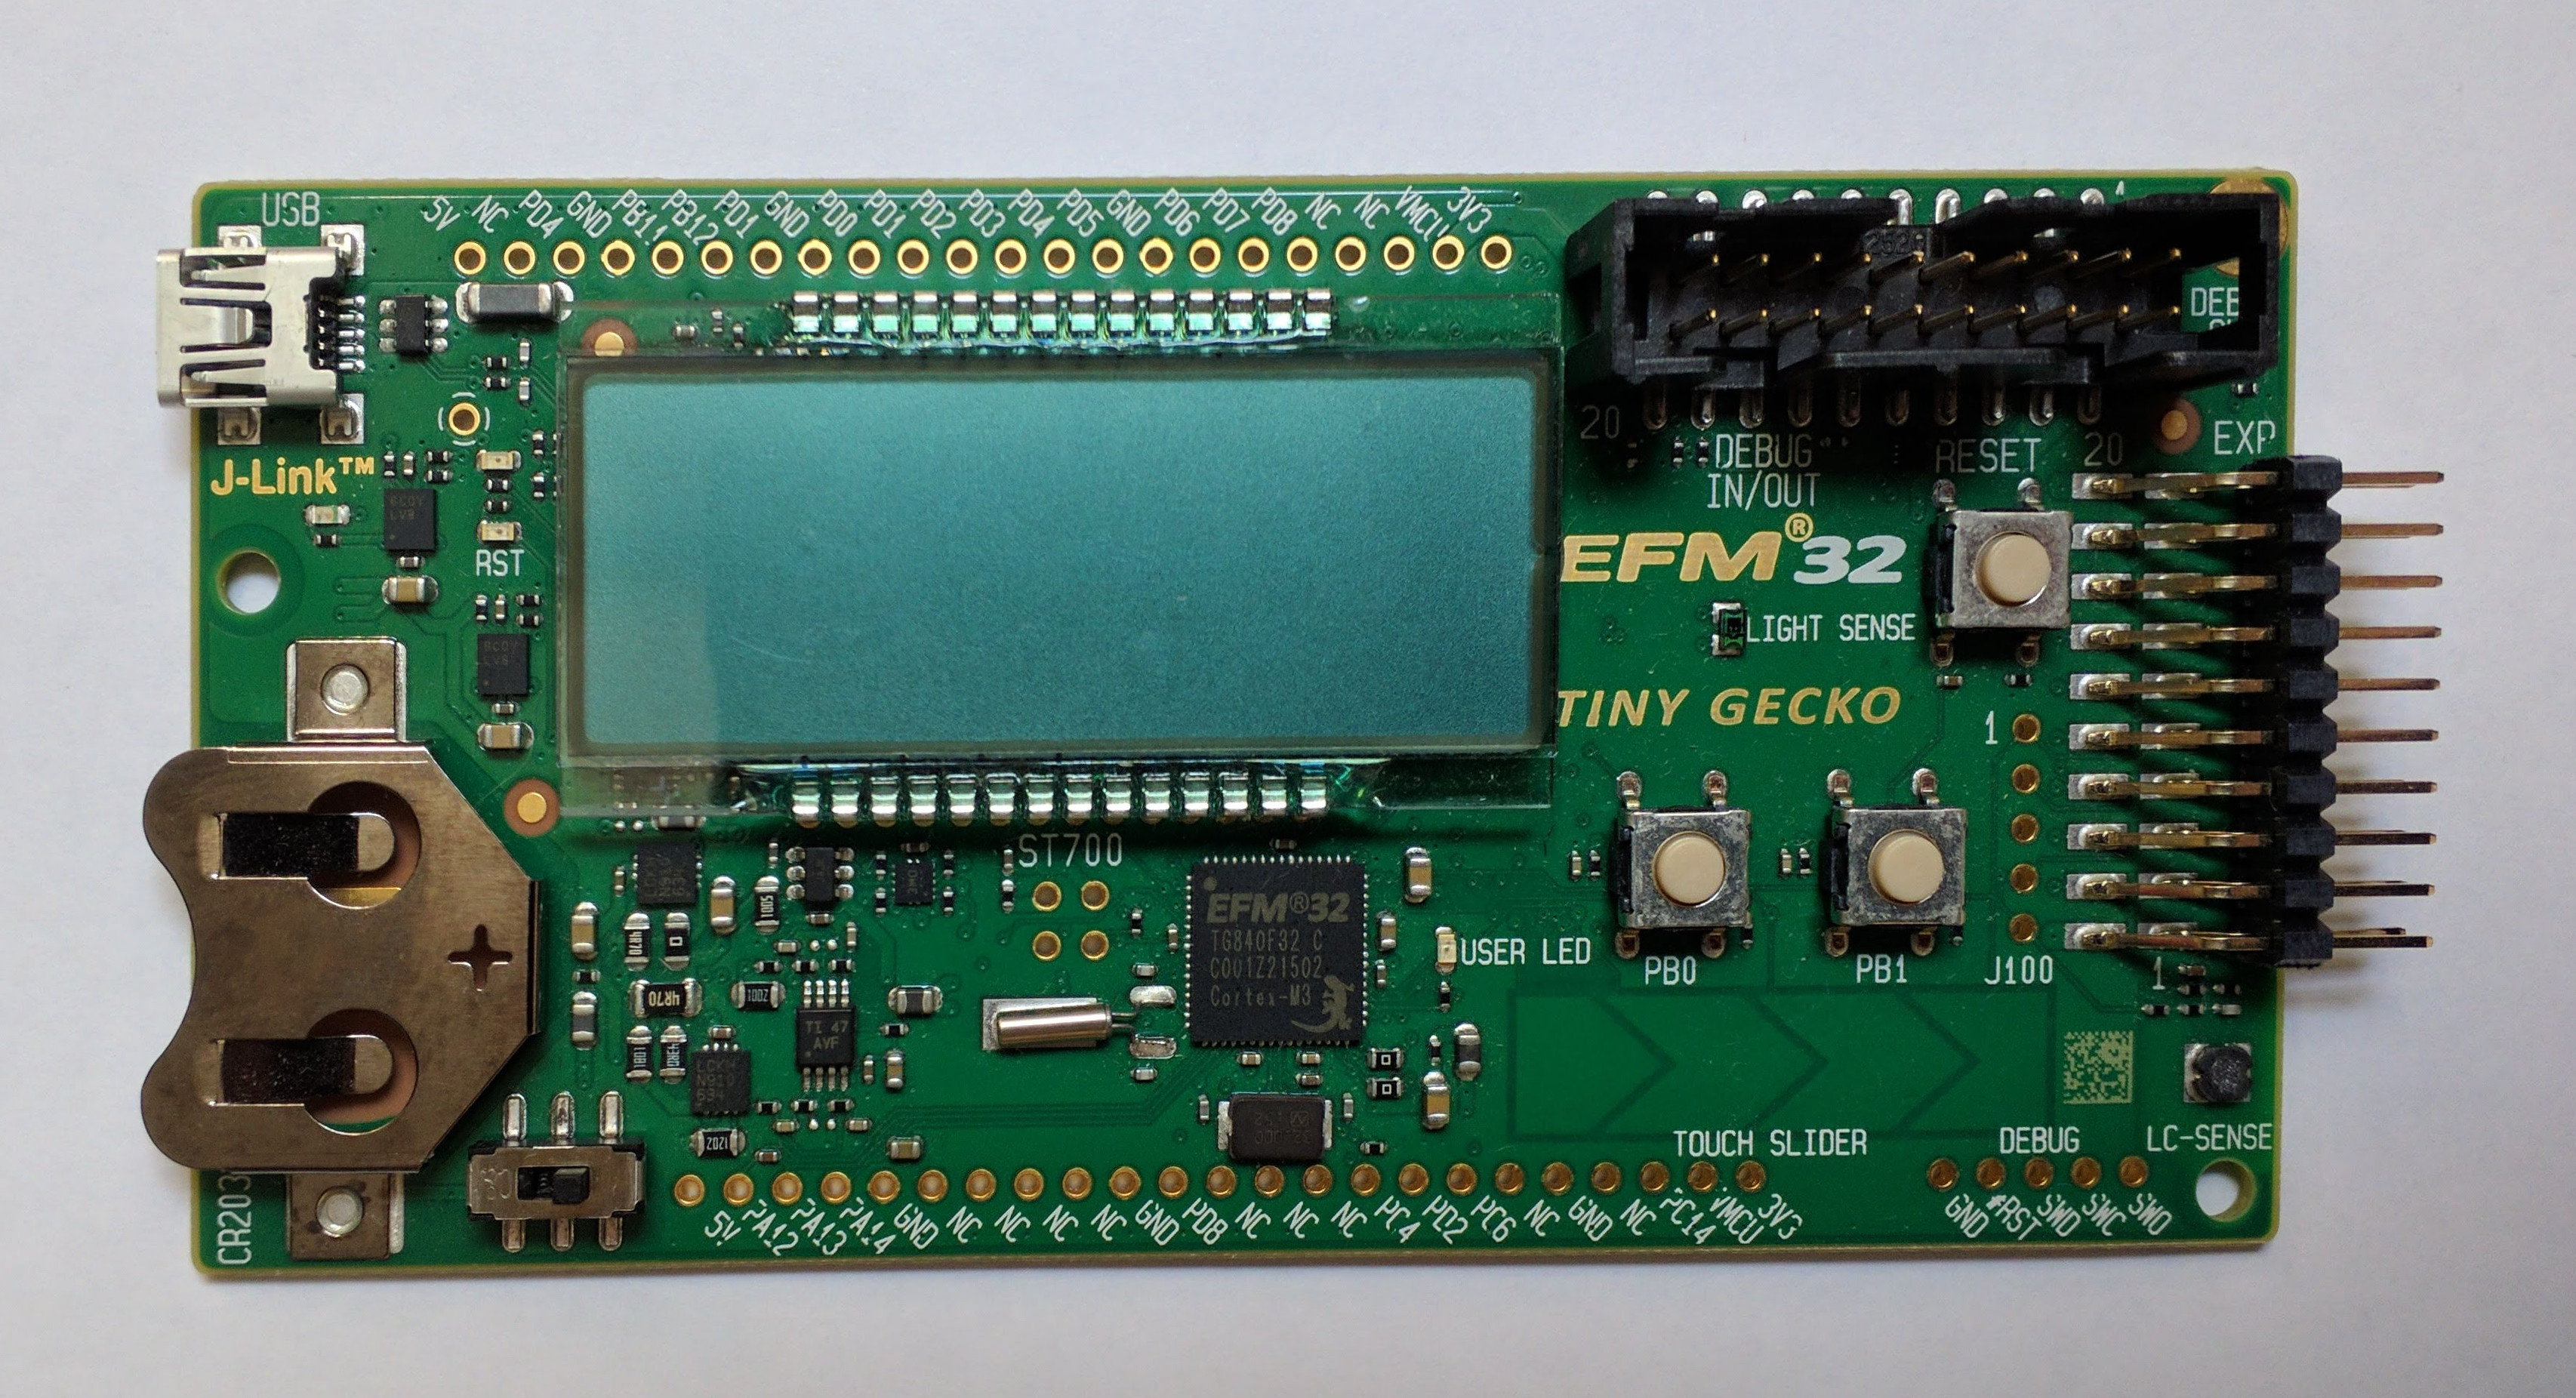
\includegraphics[width=0.85\textwidth, keepaspectratio]{imatges/tiny-gecko-starter-kit.jpg}
 \caption{Fotografia de la placa de desenvolupament de SiliconLabs}
 \label{fig:EFM32_DVK}
\end{figure}


\subsection{Dispositius auxiliars}
Per tenir dades variades i de diferent natura per les aplicacions d'exemple, farem servir els següents dispositius auxiliars:
\begin{itemize}
 \item Potenciòmetre: aquest component, que és una resistència variable, ens permetrà probar un \gls{ADC}
 \item Sensor de llum, color i moviment APDS-9960 \cite{apds9960}. Es pot adquirir a qualsevol botiga on-line ja muntat a una \gls{PCB} que incorpora uns connectors senzills per connectar-la a la PCB de desenvolupament.
 \item Cables de connexió tipus Dupont amb connector femella als dos extrems (Figura~\ref{fig:dupont}).
\end{itemize}

\begin{figure}
 \centering
 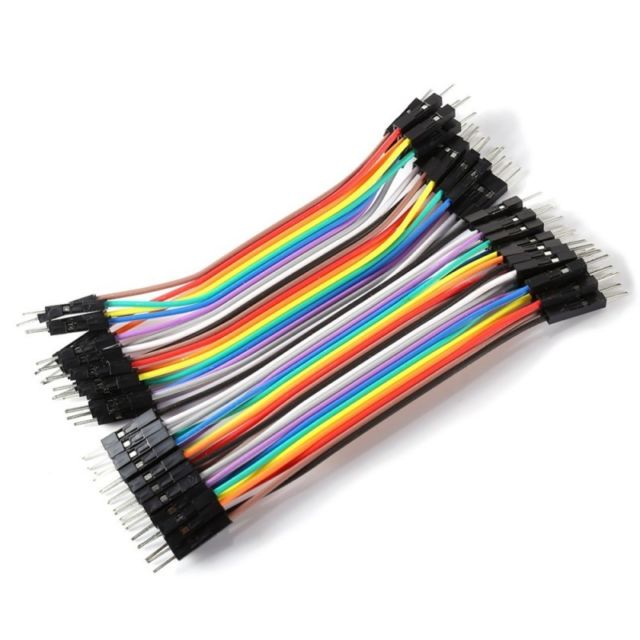
\includegraphics[width=0.45\textwidth, keepaspectratio]{imatges/cables_dupont.jpg}
 \caption{Cables dupont}
 \label{fig:dupont}
\end{figure}

\section{Eines}

Per treballar amb microcontroladors ens calen un conjunt d'eines específiques i algunes de més genèriques. Anem a veure-les amb un cert detall.

\subsection{Programadors i {\em debuggers}}
Un microcontrolador (també dit \gls{MCU} o \textmu C) es diferència d'un processador de propòsit general en moltes coses, però una de les diferències més notables és que el propi microcontrolador generalment incorpora la seva pròpia memòria (tanta \gls{RAM} com \gls{ROM}) on s'emmagatzema el codi a executar i les variables i dades a tractar. Quan el microcontrolador s'engega comença a executar el codi que troba a la ROM a certa posició.

Per descarregar el fitxer binari a la ROM, cal un dispositiu extern al microcontrolador que emmagatzema el fitxer a la ROM del microcontrolador. Aquests dispositius poden ser totalment externs al nostre circuit, i es coneixen com programadors o darrerament es veuen incorporats a la pròpia \gls{PCB} i s'hi accedeix via USB. Sigui com sigui, cal aquest programador per gravar la memòria FLASH (que funciona com una ROM pel microcontrolador).

A més, aquest programador sol afegir característiques de {\em debug}, de manera que podem controlar l'execució del microcontrolador, inspeccionar el valor de variables o posicions de memòria, accedir a la consola de {\em debug}, etc.

\subsection{Toolchain}
Com per tot processador, cal un seguit d'eines que ajudin a traduir el nostre codi (normalment C o C++) en instruccions màquina que la CPU pugui processar. Aquestes eines son el compilador i el {\em linker}. El compilador fa aquesta traducció pròpiament dita i genera fitxers objecte i el {\em linker} recull tot de fitxers objecte per crear un sol fitxer executable o biblioteca.

En el cas dels microcontroladors, hem d'acabar obtenint un fitxer executable que serà el que el microcontrolador començarà a executar quan s'engegui. Aquest fitxer haurà de tenir tot el conjunt de biblioteques i funcions necessàries per la correcta execució de l'aplicació, ja que en aquest context no tenim cap mena de sistema operatiu que ens proporcioni cap ajuda ni biblioteques.

També és habitual disposar d'algun \gls{IDE} que ens agrupa totes les eines en un entorn amigable i senzill (veure~Figura~\ref{fig:IDE}.)

\begin{figure}
 \centering
 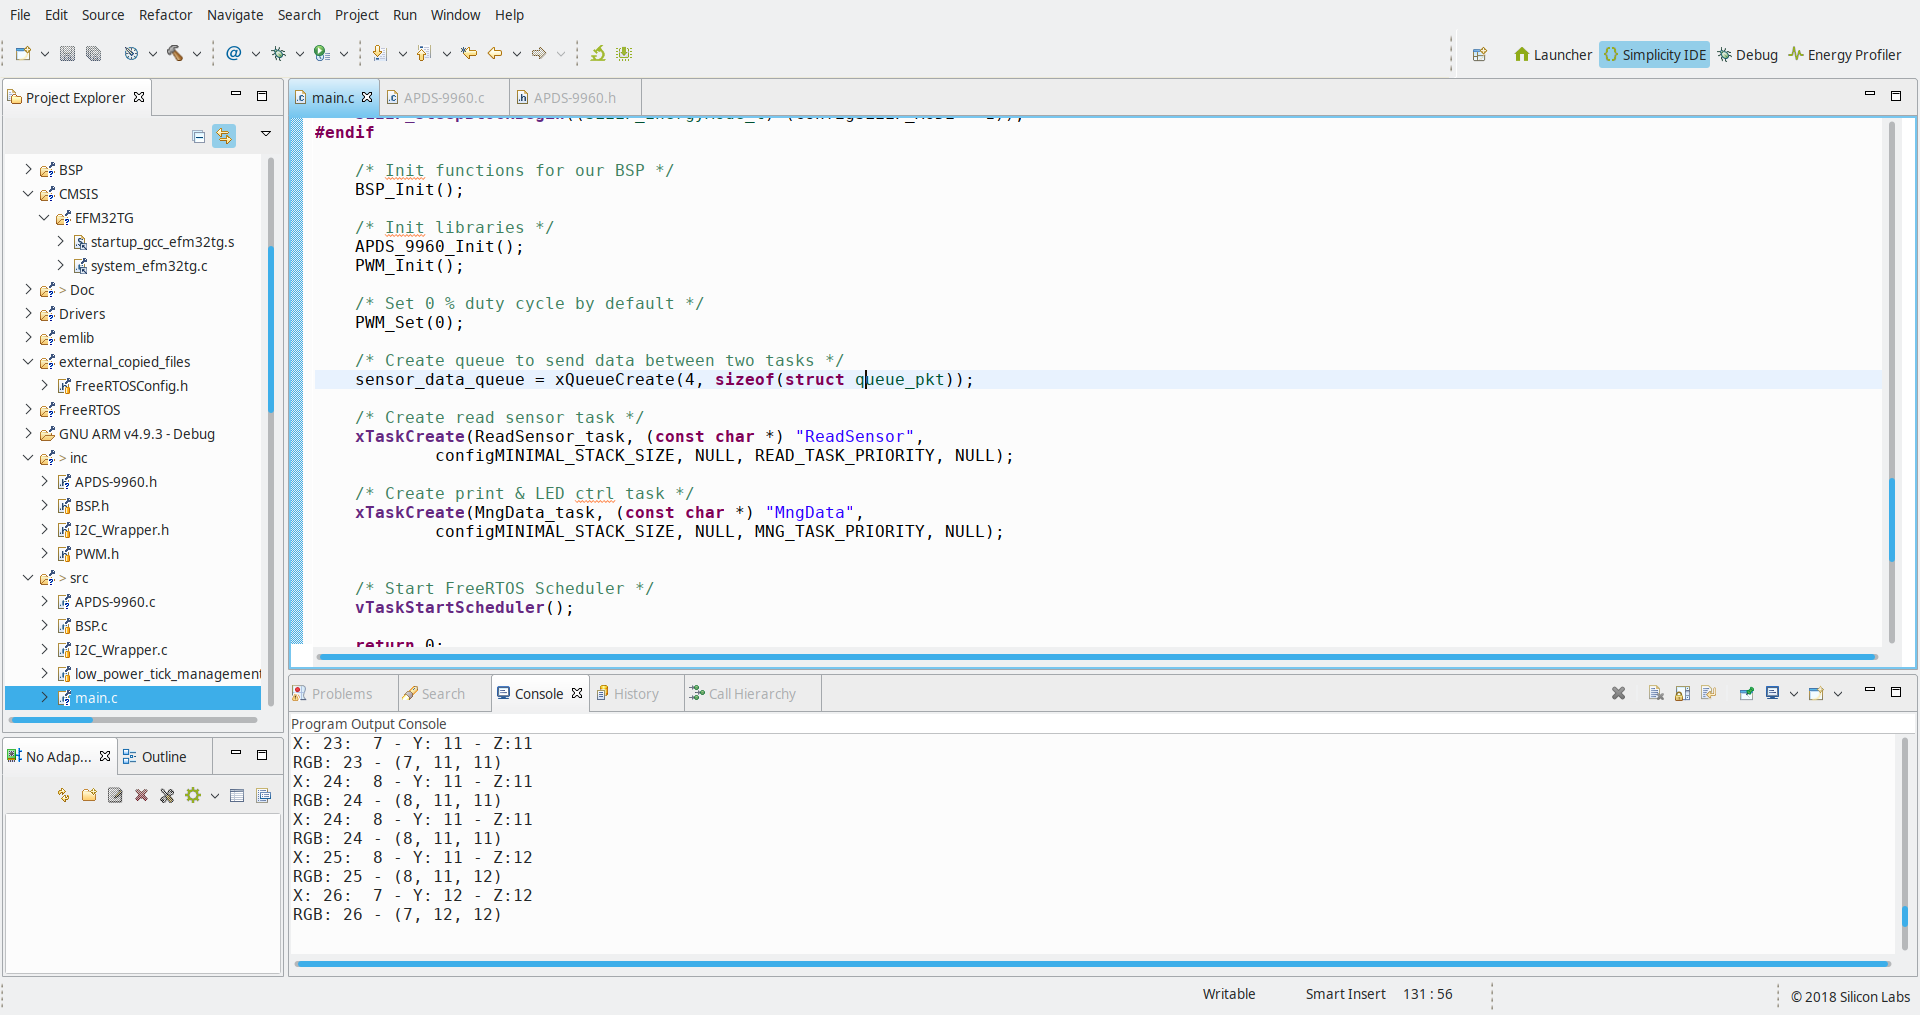
\includegraphics[width=0.85\textwidth, keepaspectratio]{imatges/capturaIDE.png}
 \caption{Aspecte del IDE Simplicity Studio\texttrademark de SiliconLabs}
 \label{fig:IDE}
\end{figure}

L'\gls{IDE} de Simplicity fa servir com a compilador el compilador per ARM de GNU \cite{ARMGNU}. Aquest compilador és de codi obert i lliure i és àmpliament utilitzant per la majoria de fabricants a les seves eines.


%% Capitol 2 - Descripció dels diferents components d'un sistema encastat: Microcontroladors, perifèrics, busos

\chapter{Breu introducció als sistemes encastats}
\label{ch:components}

Un sistema encastat és, bàsicament, un seguit de components hardware i software treballant conjuntament per obtenir una aplicació o funcionalitat determinada.

Els components hardware es poden dividir en tres grans blocs:
\begin{itemize}
\item Procés de dades: dispositiu amb la capacitat de gestionar dades, entrada sortida, etc. Pot ser un microcontrolador, un \gls{DSP}, una \gls{FPGA}, un \gls{ASIC} o un sistema hibrid que incorpori varis dels anteriors dins el mateix hardware.
 \item Sensors o introducció de dades. Qualsevol dispositiu que rep estímuls del mon físic i els converteix en dades, ja siguin digitals o analògiques (termòmetre, pantalla tàctil, acceleròmetre, etc.).
 \item Actuadors o presentació de dades. Qualsevol dispositiu que rep una dada o sèrie de dades i ho converteix en una acció física (motor, pantalla, relé, etc.).
\end{itemize}


\section{Microcontroladors}
Un microcontrolador està compost bàsicament d'una \gls{CPU}, memòria \gls{RAM} i \gls{ROM}, i un seguit de perifèrics tot integrat en un sol dispositiu. La varietat de microcontroladors diferents que es poden trobar al mercat és ingent, fent impossible fer un llistat de totes les opcions disponibles.

Històricament cada fabricant de microcontroladors tenia les seves pròpies famílies de dispositius (amb la seva pròpia arquitectura) amb les eines necessàries i, habitualment, cada conjunt era diferent i incompatible amb els demès.
Durant els últims anys aquest panorama ha canviat força, ja que molts fabricants han acabat adoptant una sola arquitectura. Aquesta arquitectura és l'anomenada {\bf \gls{Cortex}} de l'empresa \gls{ARM} \cite{Cortex}. Els fabricants trien quin model de CPU volen incorporar al seu dispositiu i hi afegeixen els perifèrics del seu catàleg que consideren que cal a cada dispositiu concret. D'aquesta manera, un sol fabricant té desenes o centeners de dispositius diferents basats en una mateixa CPU i amb diferents combinacions i nombre de perifèrics i memòria.

Tot i que tenim diferents dispositius de diferents fabricants que poden tenir la mateixa CPU, un executable no serà compatible entre aquests dispositius, ja que, segurament, el mapa de memòria o els diferent perifèrics seran diferents i, per tant, incompatibles.

Alguns dels fabricants més reconeguts de microcontroladors actuals són els següents:
\begin{itemize}
 \item \acrfull{Silabs} \cite{SiLabs}
 \item \acrfull{TI} \cite{TI}
 \item \acrfull{NXP} \cite{NXP}
 \item \acrfull{ST} \cite{ST}
 \item Microchip, antiga Atmel \cite{Microchip}
\end{itemize}

\section{ARM Cortex}
\label{sec:cortex}
Com ja hem dit, l'arquitectura \gls{Cortex} és actualment una de les més esteses en el camp dels processadors i microcontroladors de 32 bits. Es presenten tres perfils diferents segons l'àmbit d'aplicació:
\begin{itemize}
 \item {\bf Cortex-A} (d'{\bf A}plicació) Processadors d'altes prestacions per usos en telèfons mòbils, servidors, {\em tablets}, etc. \cite{CortexA}.
 \item {\bf Cortex-R} (de Temps {\bf R}eal) Dissenyats per aplicacions amb alts requeriments de seguretat com dispositius mèdics, aviònica o \glspl{PLC} \cite{CortexR}.
 \item {\bf Cortex-M} (de {\bf M}icrocontrolador) CPUs dissenyats per microcontroladors i aplicacions de baix consum \cite{CortexM}.
\end{itemize}

En aquest llibre i curs ens centrarem exclusivament a parlar del Cortex-M i les seves versions.

\begin{figure}
 \centering
 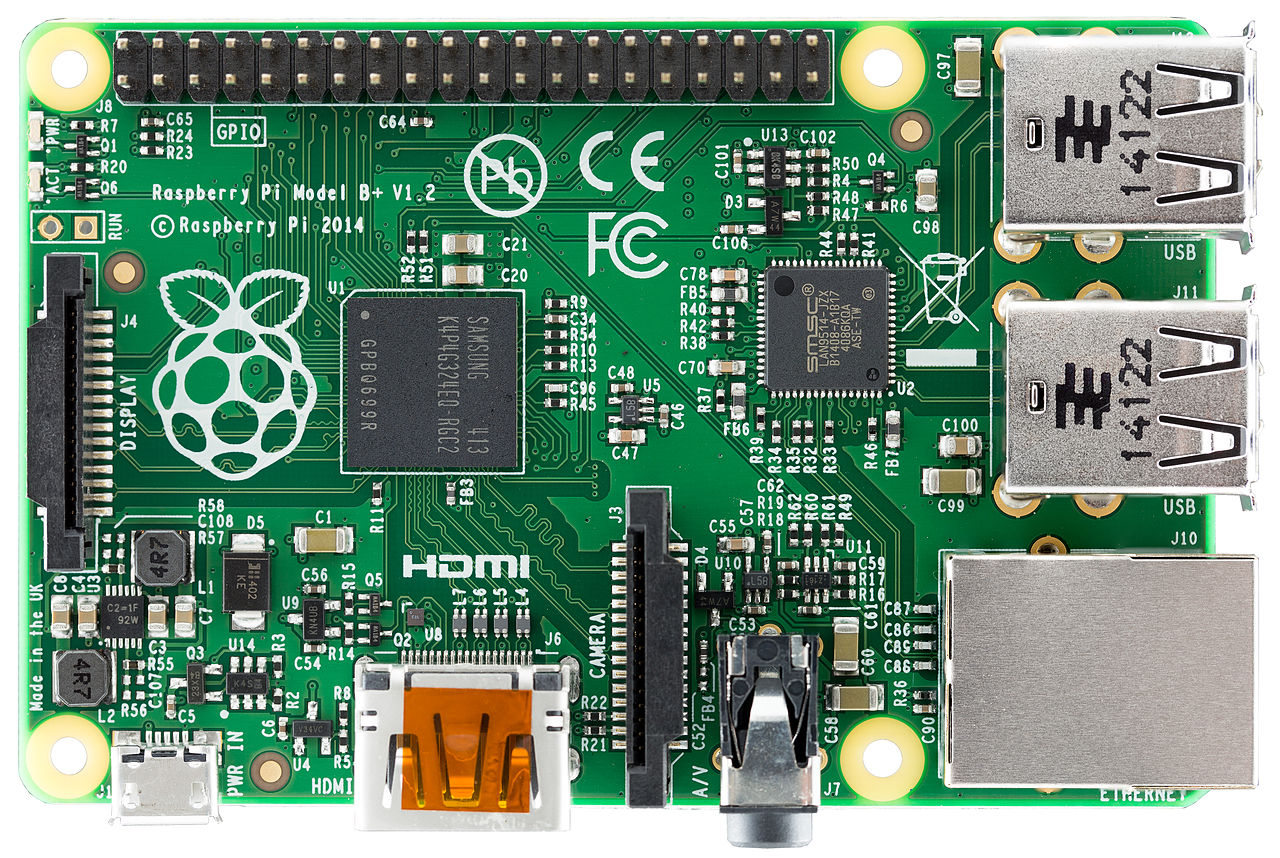
\includegraphics[width=0.65\textwidth, keepaspectratio]{imatges/Raspberry_Pi}
 \caption{Raspberry Pi amb un processador Cortex-A}{Raspberry Pi amb un processador Cortex-A. Per Lucasbosch [CC BY-SA 3.0], de la Wikimedia Commons \url{https://upload.wikimedia.org/wikipedia/commons/thumb/6/6f/Raspberry_Pi_B\%2B_top.jpg/512px-Raspberry_Pi_B\%2B_top.jpg}}
 \label{fig:Raspberry_Pi}
\end{figure}

\subsection{Cortex-M}
Aquesta arquitectura proposada per ARM és una arquitectura tipus RISC de 32 bits amb suport de {\em cache}, punt flotant i dissenyada per ser de baix consum. Tot i que hi ha diferents versions d'aquesta arquitectura, mantenen un conjunt d'instruccions comuns. Aquí llistem els més habituals \cite[7]{EmbeddedBook}:

\begin{itemize}
 \item {\bf Cortex-M0+}: És la versió més bàsica d'aquesta arquitectura, orientat a dispositius molt barats i senzills. Conté un {\em pipeline} de 2 etapes i no té cap mena de {\em cache}. És la versió més senzilla que es pot trobar als catàlegs dels fabricants \cite{CortexM0}.
 \item {\bf Cortex-M3}: Versió de millors prestacions, amb un {\em pipeline} més llarg (3 etapes) i predicció de salts, suport HW d'operacions amb punt fix, sistema de debug avançat i, opcionalment, protecció de memòria \cite{CortexM3}.
 \item {\bf Cortex-M4}: Versió que afegeix capacitats de punt flotant en HW a un Cortex-M3 \cite{CortexM4}.
 \item {\bf Cortex-M7}: Versió d'alt rendiment amb un {\em pipeline} de 6 etapes superescalar, predicció de salts i aritmètica de punt flotant de fins a 64 bits \cite{CortexM7}.
\end{itemize}

\begin{table}
\caption{Rendiment de diferents famílies de Cortex-M \cite[22]{DesignersGuide}}
\centering
\begin{tabular}{lllll}
 & M0+ & M3 & M4 & M7\\
Dhrystone (DMIPX/MHz) & 0.94 & 1.25 & 1.25 & 2.14\\
CoreMark/MHz & 2.42 & 3.32 & 3.40 & 5.04\\
\end{tabular}
\label{tab:ARMPerformances}
\end{table}



\begin{figure}
 \centering
 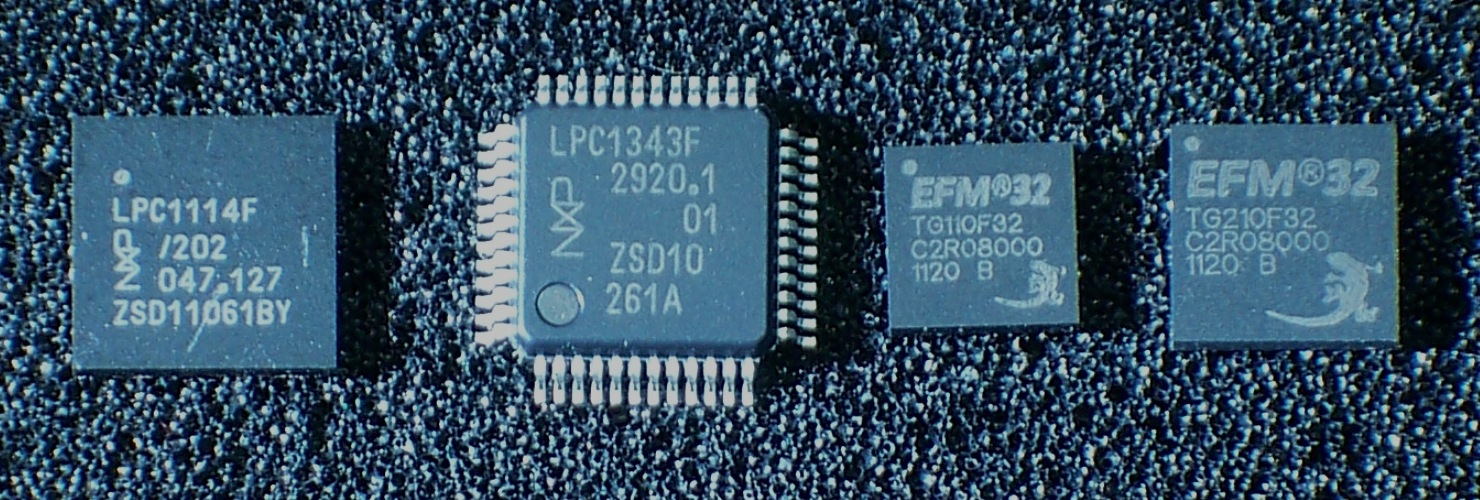
\includegraphics[width=0.65\textwidth, keepaspectratio]{imatges/ARM_Cortex-M0}
 \caption{Diferents microcontrolador Cortex-M0 i M3}{Diferents microcontrolador Cortex-M0 i M3. Per Viswesr [CC BY-SA 3.0], de la Wikimedia Commons \url{https://upload.wikimedia.org/wikipedia/commons/thumb/3/3d/ARM_Cortex-M0_and_M3_ICs_in_SMD_Packages.jpg/512px-ARM_Cortex-M0_and_M3_ICs_in_SMD_Packages.jpg}}
 \label{fig:STAsic}
\end{figure}

\begin{figure}
 \centering
 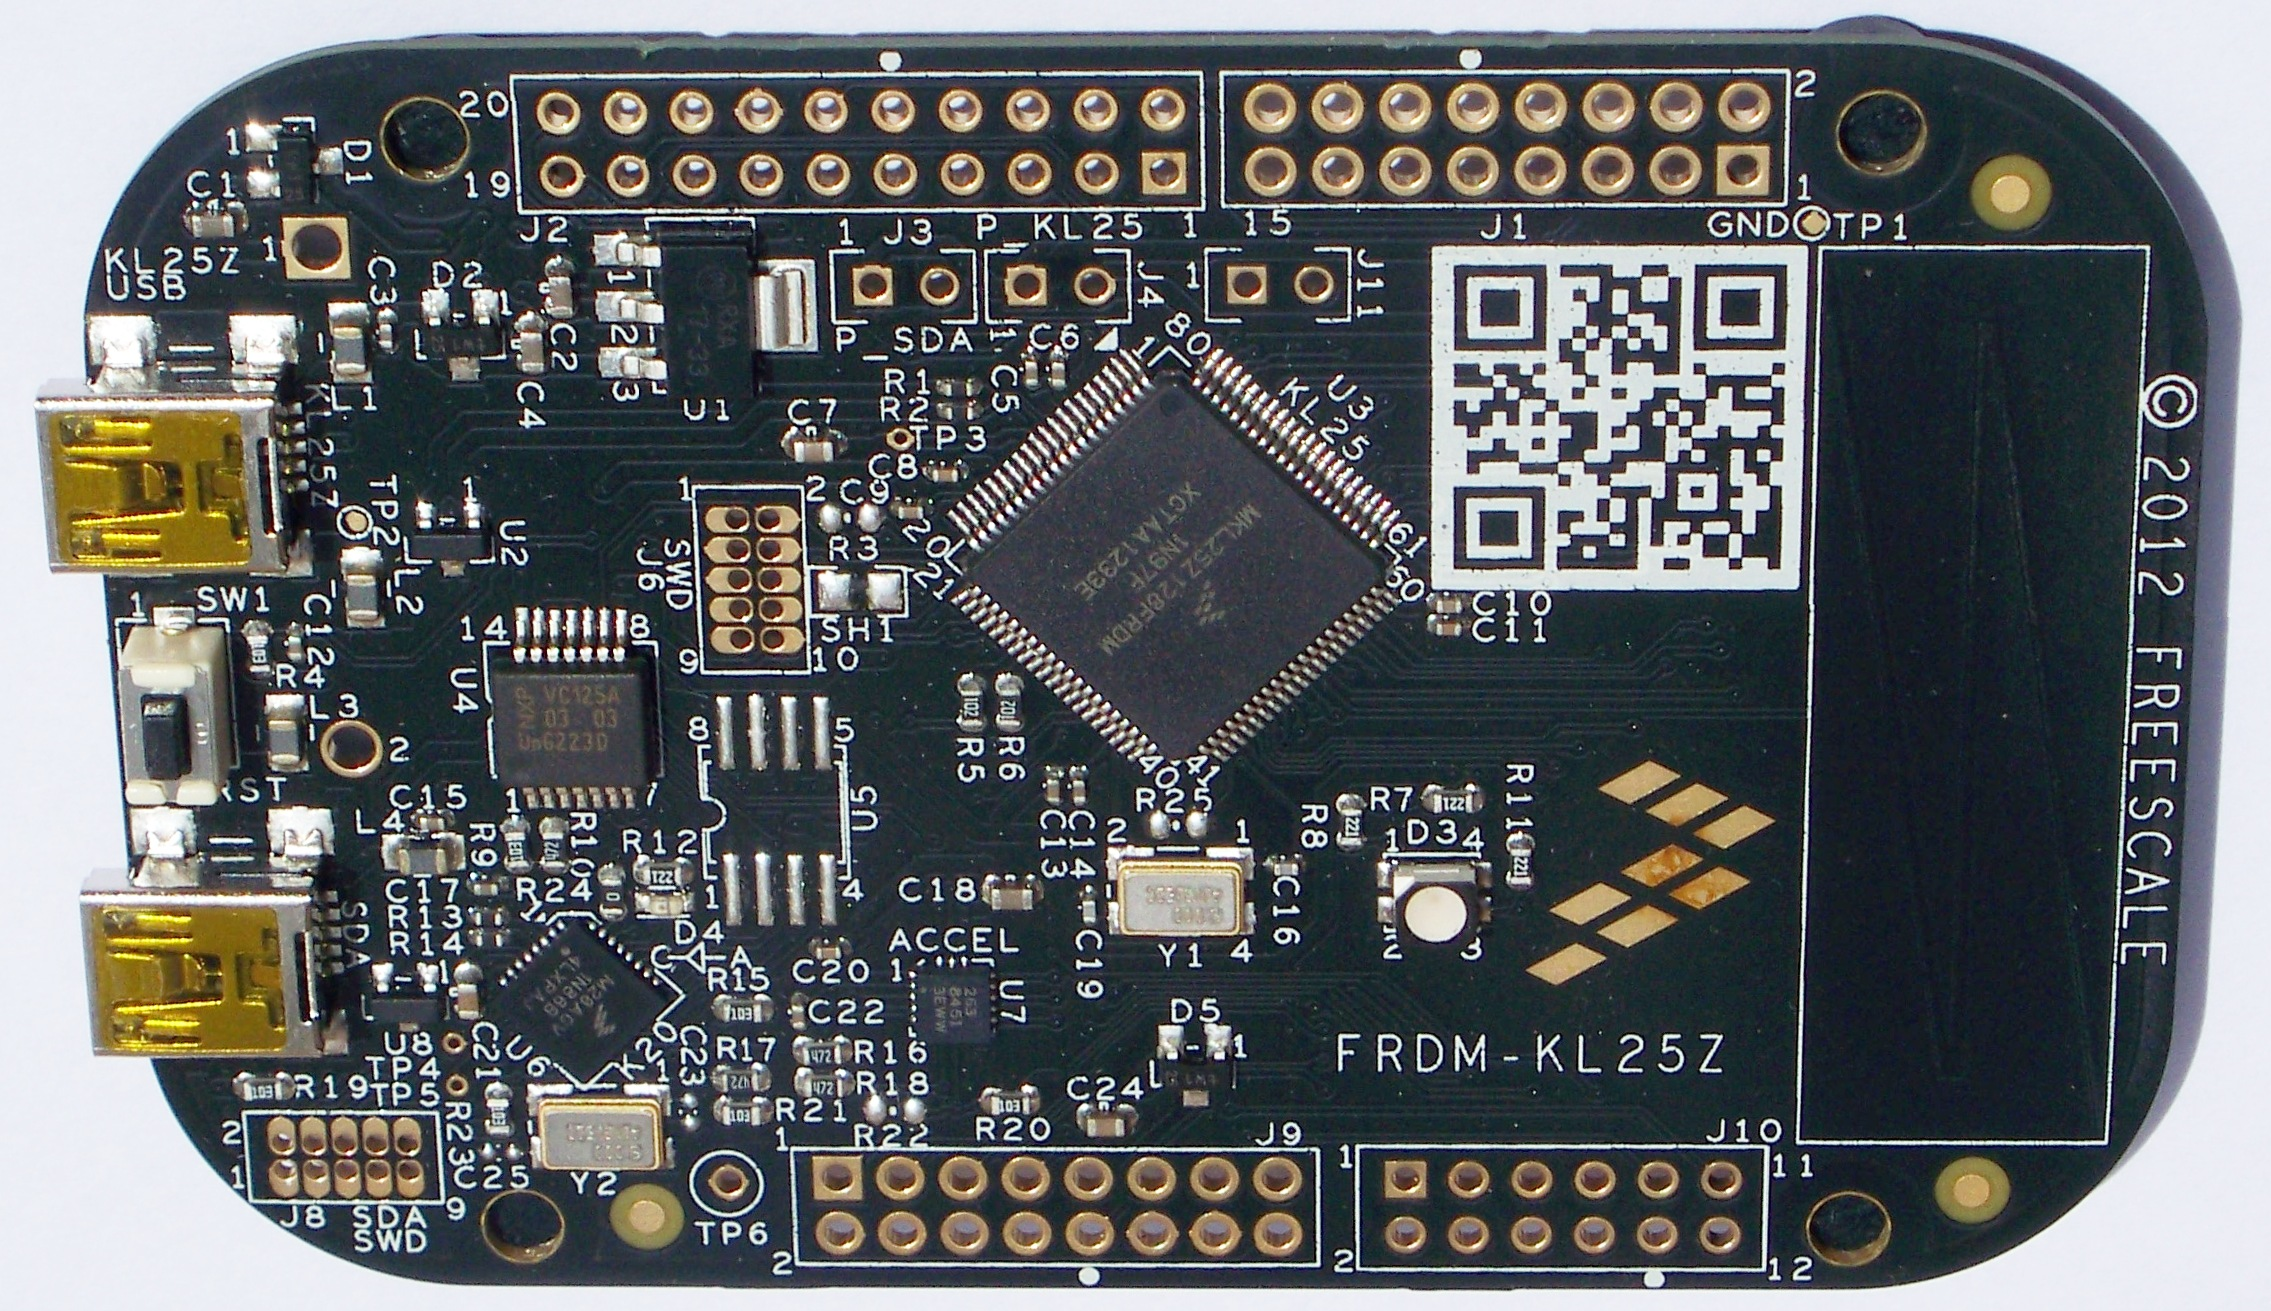
\includegraphics[width=0.65\textwidth, keepaspectratio]{imatges/Freescale_FRDM-KL25Z}
 \caption{Placa Freescale FRDM-KL25Z amb un Cortex-M0+}{Placa Freescale FRDM-KL25Z amb un Cortex-M0+. Per Viswesr [CC BY-SA 3.0], de la Wikimedia Commons \url{https://commons.wikimedia.org/wiki/File:Freescale_FRDM-KL25Z_board_with_KL25Z128VLK_(ARM_Cortex-M0\%2B_MCU).JPG}}
 \label{fig:FRDM}
\end{figure}


\section{Arquitectura}
\label{se:arquitectura}
L'arquitectura dels processadors Cortex-M varia segons la família que estudiem. La família Corte-M0+ té una arquitectura Von Newmann i la resta de famílies tenen arquitectura Harvard mixta, on tot i que la CPU té busos separats per accedir a l'espai de dades o a l'espai de codi, estan tots dos connectats a uns sola matriu (Figura~\ref{fig:M3MemoryMap}) \cite[794]{GuideCortexM3M4}.

A part de la CPU pròpiament dita, el que se'n diu {\em core} en els microcontroladors ARM inclou també un controlador d'interrupcions (veure~\fullref{ch:IRQ}), un {\em timer} simple (\fullref{sec:systick}) i un mòdul opcional de protecció de memòria (MPU) \cite[230]{GuideCortexM3M4}. Al ser dispositius comuns a tots els {\em Cores}, l'accés a ells és molt similar entre diferents fabricants (veure \fullref{sec:CMSIS-Core}).

\subsection{Perifèrics mapats a memòria}
\label{sub:memory-mapped}
A l'arquitectura Cortex els perifèrics estan mapats a memòria (\gls{memory mapped}). Això fa que tinguem accessibles els registres de cada perifèric a una regió de memòria determinada. Així doncs, per accedir als registres d'un perifèric per configurar-lo o accedir a les seves dades el que caldrà fer és accedir a una certa adreça de memòria de la forma habitual i llegir o escriure la dada que pertoqui. Aquest mapa de memòria depèn de cada fabricant i model.

\begin{figure}
 \centering
 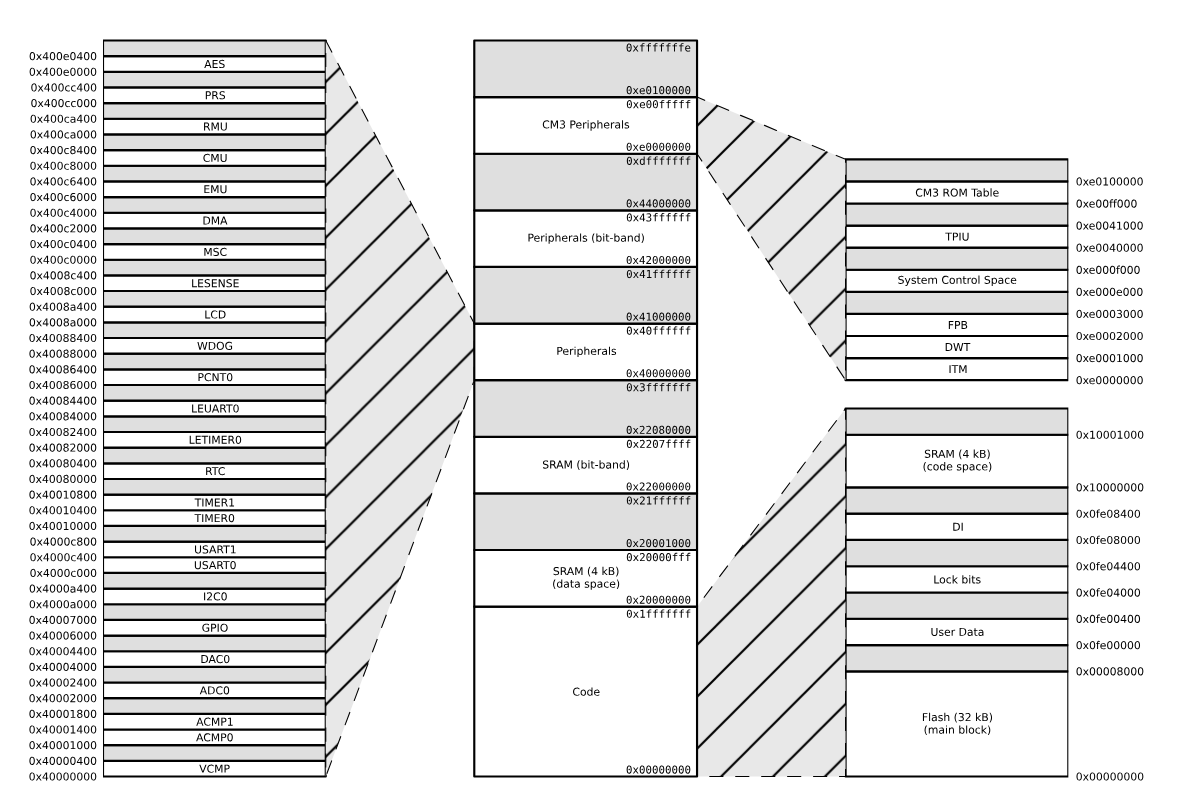
\includegraphics[width=0.85\textwidth, keepaspectratio]{imatges/Cortex-M3-MemoryMap.png}
 \caption{Mapa de memòria d'un Cortex-M3}{Mapa de memòria d'un Cortex-M3 (EFM32TG Reference Manual \cite{EFM32GRM} \copyright SiliconLabs)}
 \label{fig:M3MemoryMap}
\end{figure}

Per exemple, en el Cortex-M3 de la nostra placa, el mapa de memòria és el següent (resumit) (Figura~\ref{fig:M3MemoryMap}):
\begin{itemize}
\item de 0x0000\_0000 fins a 0x1FFF\_FFFF: Codi, aquí hi ha mapat la Flash del microprocessador, incloent-hi la memòria de codi principal, i alguna zona tipus FLASH per l’usuari.
\item de 0x2000\_0000 fins 0x2000\_3FFF la memòria RAM del microprocessador.
\item de 0x4000\_0000 fins 0x40FF\_FFFF estan mapats tots els perifèrics que conformen el microcontrolador. Per exemple:
\begin{itemize}
\item 0x4000\_6000 fins 0x4000\_6FFF hi ha el controlador de \gls{GPIO}
\item 0x4000\_2000 fins 0x4000\_2FFF hi ha l’ADC0.
\item 0x4000\_6000 fins 0x4000\_6FFF hi ha el controlador de GPIO
\end{itemize}
\item etc.
\end{itemize}

Dins de la primera zona hi trobem la zona DI ({\em Device Information}) de l’adreça 0x0FE0\_8000 fins a 0x0FE0\_8400. Aquesta zona guarda certs valors únics per a cada dispositiu. En aquest espai, els registres MEM\_INFO\_FLASH, MEM\_INFO\_RAM i PART\_FAMILY els podem llegir fàcilment \cite[24]{EFM32GRM} (Figura~\ref{fig:EFM32_DI}):

\begin{figure}
 \centering
 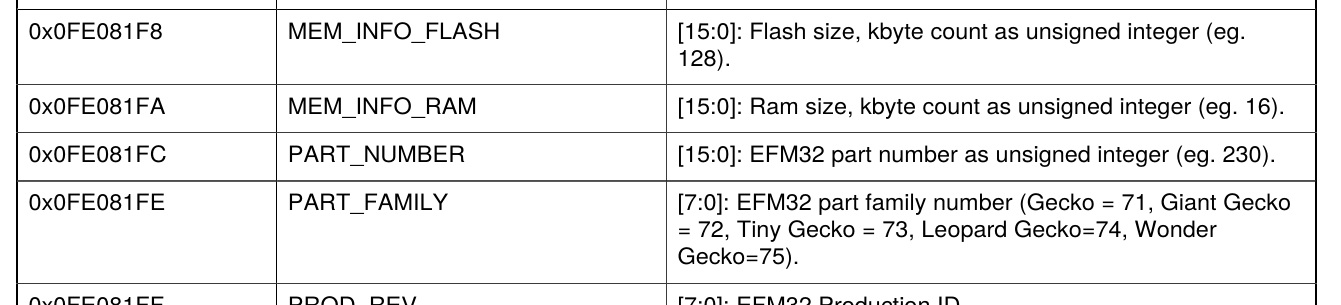
\includegraphics[width=0.85\textwidth, keepaspectratio]{imatges/DI_Table_RM.png}
 \caption{Registres de la DI a usar a l'exemple \cite[24]{EFM32GRM}}
 \label{fig:EFM32_DI}
\end{figure}



\begin{lstlisting}[frame=single,caption={Accedint a memòria en C},label=memorymappedCode,style=customc]
#define FLASH_INFO  (*(unsigned char *)0x0FE081F8)
#define RAM_INFO    (*(unsigned char *)0x0FE081FA)
#define PART_INFO   (*(unsigned char *)0x0FE081FE)

volatile uint32_t aux;

int main(void) {
  while (1) {
    aux = FLASH_INFO; /* 32 kB */
    aux = RAM_INFO;   /* 4 kB */
    aux = PART_INFO;  /* 73 = Tiny Gecko */
  }
}
\end{lstlisting}

Al codi del Llistat~\ref{memorymappedCode} es defineixen les 3 adreces de memòria per ser accedides fent servir un punter. Així, llegint el valor de les definicions FLASH\_INFO, RAM\_INFO o PART\_INFO s’accedeix a la posició de memòria definida de forma directa. Per fer una escriptura es faria igual, però en l'exemple no es pot escriure a cap d'aquests registres. Debugant el codi línia a línia veurem que la variable aux pren el valor corresponent a cada un dels registres mapats.

Enlloc d'accedir a cada registre per separat, com hem fet a l'exemple, es pot definir una estructura que es correspongui amb cada un dels registres d’un perifèric en concret i que aquesta apunti a l'adreça base del perifèric. Així, per accedir a un registre en concret només caldrà accedir al camp de l'estructura definida.

Un exemple d'això el tenim a fitxer efm32g\_devinfo.h, que defineix
una estructura d'aquest estil, com es veu al llistat~\ref {devinfo}.

\begin{lstlisting}[label=devinfo,caption={Exemple de definició d'estructura per accedir a memòria},style=customc]
typedef struct
{
  __IM uint32_t CAL;            /**< Calibration temperature and checksum */
  __IM uint32_t ADC0CAL0;       /**< ADC0 Calibration register 0 */
  __IM uint32_t ADC0CAL1;       /**< ADC0 Calibration register 1 */
  __IM uint32_t ADC0CAL2;       /**< ADC0 Calibration register 2 */
  uint32_t RESERVED0[2];        /**< Reserved */
  __IM uint32_t DAC0CAL0;       /**< DAC calibrartion register 0 */
  __IM uint32_t DAC0CAL1;       /**< DAC calibrartion register 1 */
  __IM uint32_t DAC0CAL2;       /**< DAC calibrartion register 2 */
  __IM uint32_t AUXHFRCOCAL0;   /**< AUXHFRCO calibration register 0 */
  __IM uint32_t AUXHFRCOCAL1;   /**< AUXHFRCO calibration register 1 */
  __IM uint32_t HFRCOCAL0;      /**< HFRCO calibration register 0 */
  __IM uint32_t HFRCOCAL1;      /**< HFRCO calibration register 1 */
  __IM uint32_t MEMINFO;        /**< Memory information */
  uint32_t RESERVED2[2];        /**< Reserved */
  __IM uint32_t UNIQUEL;        /**< Low 32 bits of device unique number */
  __IM uint32_t UNIQUEH;        /**< High 32 bits of device unique number */
  __IM uint32_t MSIZE;          /**< Flash and SRAM Memory size in KiloBytes */
  __IM uint32_t PART;           /**< Part description */
} DEVINFO_TypeDef; /** @} */
\end{lstlisting}

Que es correspon amb els registres de la regió DI a la que hem accedit abans. Aquesta estructura es fa servir al fitxer efm32tg840f32.h definint la referència mostrada al llistat~\ref {devinfodec}.

\begin{lstlisting}[label=devinfodec,caption={Declaració d'una variable d'accés a la memòria estructurada},style=customc]
#define DEVINFO ((DEVINFO_TypeDef *) DEVINFO_BASE) /**< DEVINFO base ptr */
\end{lstlisting}

De manera que es pot accedir als mateixos registres com s'indica al
llistat~\ref {devinfouse}. Que és una forma bastant més còmoda de treballar.

\begin{lstlisting}[label=devinfouse,caption={Ús de l'estructura d'accés},style=customc]
aux = DEVINFO->MSIZE;
aux = DEVINFO->PART;
\end{lstlisting}

Per sort, la majoria de fabricants proporcionen llibreries de baix nivell que ens estalvien tant conèixer tots els detalls de cada un dels perifèrics com d'haver de manegar els registres un a un: pel cas de SiliconLabs aquestes llibreries s'agrupen sota la EMLIB \cite{EMLIB}; en el cas de l'empresa ST ens proporciona la biblioteca {\em STM32 Standard Peripheral Libraries} \cite{STM32Lib} o la més moderna {\em  STM32Cube hardware abstraction layer (HAL)} \cite{STM32CubeHAL}.

% \fbox{El codi d'aquest exemples està al \href{https://github.com/mariusmm/cursembedded/tree/master/Simplicity/MemoryMap}{repositori del curs}}

El codi d'aquests exemples està al \href{https://github.com/mariusmm/cursembedded/tree/master/Simplicity/MemoryMap}{repositori del curs}

\subsection{Mida del codi i seccions de memòria}
\label{sub:size}
Quan compilem el nostre codi, com ja sabem, el compilador trasllada el codi C i assemblador a codi màquina, generant un fitxer per cada mòdul que formi l'aplicació (anomenats fitxers objecte amb extensió .o). A continuació el {\em linker} agafa tots els fitxers objecte i crea el fitxer binari tipus ELF.

En aquest fitxer hi ha tota la informació necessària per programar el microcontrolador, i això inclou el codi màquina que cal executar, les definicions de les variables i la seva inicialització, el codi d'inicialització (veure \fullref{sub:boot}), etc. Aquest fitxer serà el que després el programador o {\em debugger} llegirà per tal de programar el microcontrolador.

D'aquest fitxer podem extreure informació valuosa, com és la quantitat de memòria FLASH o RAM que necessita el nostre programa. Això ens ho diu la comanda {\em size} (en el cas del compilador \gls{GCC} per \gls{ARM} la comanda és {\em arm-none-eabi-size}) quan s'executa sobre el fitxer binari creat. La sortida d'aquest programa té el següent aspecte:

\begin{lstlisting}
text    data     bss     dec     hex filename
4976     112      48    5136    1410 SpeedTest_1.axf
\end{lstlisting}

El que està mostrant és la mida (en bytes) de cada un dels segments en que es divideix la nostra aplicació:
\begin{itemize}
 \item {\bf text}: aquest sector és el corresponent al codi executable i les constants definides; també s'inclouen aquí els vectors d'interrupció (veure \fullref{ch:IRQ}). El {\em debugger} s'encarregarà de gravar a la FLASH aquesta secció.
 \item {\bf data}: s'emmagatzemem les dades inicialitzades, com són variables han d'anar a RAM, però també cal guardar el seu valor a la FLASH, per tant, ocupen espai a totes dues memòries. El procés de {\em boot} (Veure \fullref{sub:boot}) copiarà els valors d'inicialització de la FLASH cap a la variable a la RAM.
 \item {\bf bss}: conté totes les variables no inicialitzades. Aquesta secció va a la RAM. Al procés de {\em boot} (Veure \fullref{sub:boot}) aquesta secció s'inicialitza amb zeros.
 \item {\bf dec}: és la suma dels 3 camps anteriors
 \item {\bf hex}: és el mateix valor que {\bf dec} però expressat en hexadecimal.
\end{itemize}

\subsection{Procés de {\em boot}}
\label{sub:boot}
El procés de {\em boot} és tota la seqüència de passes que fa un microcontrolador des de que s'engega fins que comença a executar la nostra funció principal {\bf main()}\index{main()}.

Quan el microcontrolador surt de l'estat de {\em reset} després d'un {\em power-up}, d'un {\em reset} extern, d'un {\em reset} pel Watchdog (veure~\fullref{sec:Watchdog}), etc. cal que s'inicialitzin un seguit de mòduls i peces abans no es pugui començar a executar el nostre codi.

A la posició de memòria 0x0000\_0000 el que hi ha és el vector d'interrupció corresponent al {\em reset} que normalment crida la funció {\bf SystemInit()}\index{SystemInit()} que inicialitza, si cal, parts crítiques del microcontrolador, com el rellotge principal. A continuació es copien les variables inicialitzades de la FLASH a la RAM (secció {\bf data}), s'inicialitza a 0 la secció coneguda com {\bf bss} i per últim crida a la funció {\bf \_start()}\index{\_start()} que acabarà cridant a la nostra funció {\bf main()}\index{main()} \cite{StartUp}. Tot això ho maneguen les eines de forma automàtica i no cal que nosaltres en tinguem cura, però va bé saber què està passant dins el microcontrolador en tot moment.


\section{Rapidesa d'un microcontrolador}
\label{sub:speedtest}
Molts cops no ens fem a la idea de com de ràpid és la CPU d’un microcontrolador. Estem acostumats a llegir i escoltar freqüències de funcionament dels microprocessadors d’escriptori o de servidor, que actualment són de Gigahertz i els nostres pobres microcontroladors van, en el millor dels casos, a uns quants pocs Megahertz. Això ens pot fer pensar que els nostres microcontroladors són lents i que no poden fer gaire coses.

Podem comprovar-ho empíricament.

A l'\href{https://github.com/mariusmm/cursembedded/tree/master/Simplicity/SpeedTest_1}{exemple SpeedTest\_1} hi ha un codi molt simple que simplement incrementa un comptador mentre es té premut el botó 0 i tot seguit imprimeix per la consola el valor al que ha arribat el comptador.
\index{main()}
\begin{lstlisting}[style=customc,caption=Codi velociat d'un microcontrolador,label=cpuspeed]
void main() {
  ...
  /* while button 0 is pressed, CPU is counting */
  while (GPIO_PinInGet(gpioPortD, 8) == 0) {
    i++;
  }

  if (i != 0) {
    printf("i = %d\n", i); i = 0;
  }
  ...
}
\end{lstlisting}

Això ens hauria de donar una idea de com de ràpid és capaç la nostra CPU de fer operacions aritmètiques simples.

Pitjant el botó molt ràpidament el comptador arriba a 8.000 i 9.000. Així que sembla que compta molt ràpid!

\subsection{Millor mesura de temps}
\label{sub:speedtest_example}
El \href{https://github.com/mariusmm/cursembedded/tree/master/Simplicity/SpeedTest_2}{segon exemple} és una mica més complicat. Per tal de mesurar el temps que es pitja el botó, farem servir un {\em Timer}, que ja ho veurem més endavant (veure \fullref{sub:Timers}). El que es fa a l'exemple és mesurar acuradament el temps que està el botó pitjat i calcular el nombre d'operacions que s'ha fet en aquell temps.

Com podem veure a la Taula~\ref{tb:SpeedTest} el nombre d’operacions per segon es manté constant independentment del temps que estiguem pitjant el botó i és un número força alt, 134.000 sumes per segon!!!

\begin{table}[t!]
\caption{Mesures de temps i sumes per segon}
\centering
\begin{tabular}{|r|c|c|c|c|}
\hline
{\bf Count} & {\bf Ticks (del Timer)} & {\bf Temps (segons)} & {\bf Count/Tick} & {\bf Count/Segon}\\
\hline
16629 & 1688 & 0,12 & 9,85 & 134.677\\
\hline
10955 & 1112	& 0,08 &	9,85	& 134.681\\
\hline
81813 & 8309	& 0,61 &	9,85	& 134.609\\
\hline
17985 & 1826 & 0,13 & 9,85 &134.651 \\
\hline
12054 &1224 & 0,09 & 9,85 & 134.653\\
\hline
269785 &27400 & 2,00 & 9,85 & 134.607\\
\hline
\end{tabular}
\label{tb:SpeedTest}
\end{table}


%----------------------------------------------------------------------------------------
% 2a i 3a Part: Programació de perifèrics
%----------------------------------------------------------------------------------------s
\part{Programació de perifèrics I}
\label{part:programacio}
%% Capitol 3
% \part{Programació de perifèrics I}
% \label{part:programacio}

En aquest capítol s'aniran introduint i explicant els perifèrics mes habituals que trobem en els microcontroladors actuals. Cada capítol constarà d'una petita introducció al perifèric en qüestió i un petit exemple amb el codi corresponent i els comentaris adients.

\begin{remark}
El tipus de codi que es veurà als exemples es coneix com {\em Baremetal} que vol dir que no es fa servir cap Sistema Operatiu, que es veurà a la \fullref{part:freertos}. Aquests sistemes es basen en les inicialitzacions necessàries i un bucle sense fi al {\bf main()}\index{main()} on es realitzen les operacions desitjades. S'acostuma a usar aquest mètode en aplicacions senzilles o en aplicacions que corren en microcontroladors poc potents o sense prou memòria com per executar còmodament un \gls{RTOS}.
\end{remark}

\chapter{Consola de Debug}
\label{sub:console}
Un de les principals diferències quan treballem amb sistemes encastats és que no tenim una consola on executem el nostre binari i podem veure quins resultats ha obtingut.

Una millora d'ARM respecte arquitectures anteriors va ser la d'incorporar ja fa temps un mecanisme de debug, a través d'un pin d'output anomenat {\em SWO} que permet enviar dades cap a una consola al nostre PC de desenvolupament.

Aquest pin {\em SWO} forma part del sistema de Debug dels Cortex anomenat ITM ({\em Instrumentation Trace Macrocell}) \cite{ITM}. Això vol dir que la majoria de microcontroladors basats en Cortex que ens trobem, siguin del fabricant que sigui portaran aquesta funcionalitat.\footnote{La majoria de Cortex-M0+ no porten aquest perifèric.}

Per poder fer servir aquesta funcionalitat, cal primer configurar el pin SWO per a que funcioni com a tal (es pot fer servir també com un \gls{GPIO} normal). Tot seguit es configura el dispositiu de trace i el mòdul ITM d'aquest. La configuració es fa a la funció {\bf setupSWOForPrint()}\index{setupSWOForPrint()}.

Un cop configurat el mòdul ITM, la funció {\bf ITM\_SendChar()}\index{ITM\_SendChar()} permet enviar caràcter a caràcter el que vulguem presentar a la consola a l'altre costat.

En el cas de Simplicity, els caràcters rebuts es presenten directament a la consola de la part d'abaix del \gls{IDE} (Figura~\ref{fig:ITM}).

\begin{figure}
 \centering
 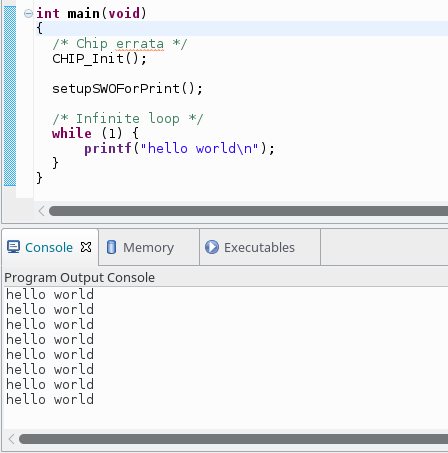
\includegraphics[width=0.85\textwidth, keepaspectratio]{imatges/ITM_Debug.png}
 \caption{Captura de pantalla de la Consola del Simplicity Studio}
 \label{fig:ITM}
\end{figure}

\chapter{Fent servir printf}
\label{sub:console_example}
Tot i que això és força útil, podem fer servir una funció força coneguda i molt útil com és {\bf printf()}\index{printf()} per fer-nos-ho tot més senzill (a canvi d'alguna cosa, com veurem).

La funció {\bf printf()} és una vella coneguda per qualsevol programador de C (o C++, o PHP, o …). Així que seria genial poder fer servir aquesta funció en el nostre sistema encastat i que la cadena aparegui a la consola del nostre PC. Això ho podem fer de la següent manera. Primer de tot cal saber que la funció {\bf printf()} fa servir la funció de sistema {\bf \_write()} per imprimir la cadena. Per tant, caldrà que implementem aquesta funció per tenir el nostre desitjat {\bf printf()}.

\index{\_write()}\index{ITM\_SendChar()}
\begin{lstlisting}[caption={Funció {\bf \_write()}},style=customc,label=write]
int _write(int file, const char *ptr, int len) {
  int x;
  for (x = 0; x < len; x++) {
    ITM_SendChar(*ptr++);
  }
  return (len);
}
\end{lstlisting}

Com podem veure al Llistat~\ref{write}, el que fa aquesta funció és anar enviant un a un tots els caràcters de la cadena passada via el paràmetre {\bf ptr} i de longitud {\bf len}.

També cal configurar el mòdul ITM (mòdul de debug) perquè activi la sortida {\em SWO} cridant a la funció {\bf setupSWOForPrint()}\index{setupSWOForPrint()}. Un cop fet això, ja podem fer servir la funció {\bf printf()}\index{printf()} tal com hem fet sempre.

Aquesta explicació la podeu trobar al \href{http://community.silabs.com/t5/Simplicity-Studio-and-Software/how-to-enable-printf-output/td-p/133981}{fòrum de Silicon Labs} (no cal registre) i el codi el teniu en el directori d'instal·lació del Simplicity/developer/sdks/exx32/v4.4.1/kits/common/drivers/ als fitxers:
\begin{itemize}
 \item retargetio.c
 \item retargetswo.c
\end{itemize}

\section{Problemes d'usar printf}
Com dèiem, poder fer servir el nostre estimat {\bf printf()}\index{printf()} al nostre sistema encastat no ens sortirà gratis. Com que aquesta funció és força complexa i permet moltes possibilitats, incloure-la en un projecte afegirà una bona quantitat de memòria de programa.

En l'exemple que tenim al repositori, les mides són les que es veuen a la Taula \ref{tb:printfsize}. Per tant, podem estimar que afegir {\bf printf()} al nostre projecte afegirà uns 3800 Bytes (3.7 KB) de codi de programa.

\begin{table}[htb]
\caption{Mida de l'executable segons {\bf printf()}}
\centering
\begin{tabular}{|c|c|}
\hline
{\bf Opció } & {\bf Bytes secció .text} \\
\hline
Sense printf() & 956\\
\hline
Amb printf() & 4.748\\
\hline
Amb printf() i punt flotant &13.644\\
\hline
\end{tabular}
\label{tb:printfsize}
\end{table}

Potser no és gaire important aquesta quantitat, però segur que caldrà tenir-la en compte si estem treballant amb microcontroladors que tenen poca memòria FLASH de programa (hi ha Cortex-M0+ amb només 4 KB de \gls{FLASH}!).

També cal tenir en compte que algunes versions de la funció {\bf printf()} no suporten valors en punt flotant. Segons l'eina, caldrà activar aquesta opció en cas que la vulguem fer servir (Figura \ref{fig:SILabsPrintfFloat}. Cal tenir en compte que això incrementarà encara més la quantitat de memòria que necessitarà aquesta funció com es veu a la Taula \ref{tb:printfsize}.

\begin{figure}[htb]
 \centering
 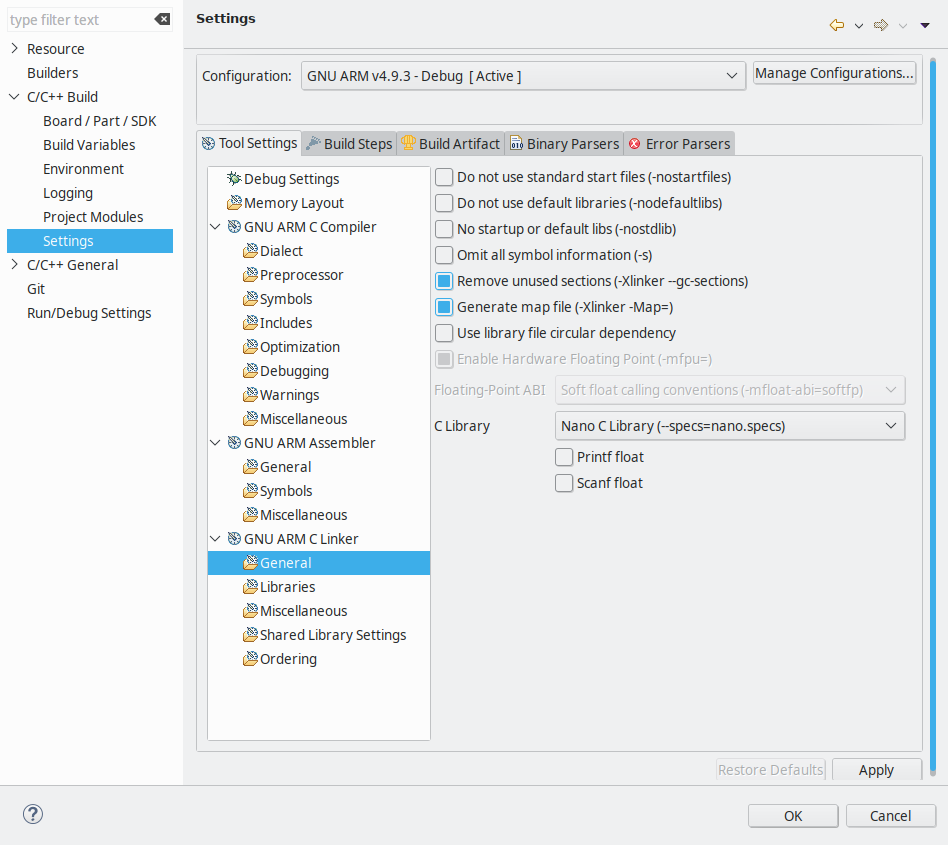
\includegraphics[width=0.85\textwidth, keepaspectratio]{imatges/SilabsPrintfFloat.png}
 \caption{Opció a {\em Simplicity} per activar el punt flotant al {\bf printf()}}
 \label{fig:SILabsPrintfFloat}
\end{figure}

Una forma força habitual de disposar dels avantatges del printf
mentre es desenvolupa i treure'l de forma ràpida quan es genera el
binari definitiu es redefinir el \textbf{printf} amb un nom nostre, i
establir una variable condicional de compilació per activar o no el
printf real, tal i com es veu en el llistat Llistat~\ref{ourprintf},
llavors en el nostre codi, enlloc de cridar \textbf{printf} per
mostrar un missatge, haurem de fer servir \textbf{PRINTF}.

\index{printf()}\index{PRINTF()}
\begin{lstlisting}[caption={Redefenir {\bf printf()}},style=customc,label=ourprintf]
#ifdef USE_PRINTF
  #define PRINTF(...) printf( __VA_ARGS__)
#else
  #define PRINTF(...)
#endif
\end{lstlisting}

\chapter{Gestió de rellotges}
\label{sec:clocks}
En la majoria de microcontroladors moderns la gestió dels rellotges és una qüestió delicada i molt important. Per tal de millorar el consum del dispositiu, és habitual tenir un control i poder decidir si cert perifèric rep el senyal de rellotge o no (més detalls a \fullref{ch:low-power}). En cas que no el rebi, el perifèric romandrà totalment desconnectat i no consumirà energia. En cas que el vulguem fer servir, una de les primeres coses que haurem de fer és activar i proporcionar-li el senyal de rellotge adequat.

Per aquesta tasca de controlar els rellotges, acostuma a existir un perifèric concret que fa tota la gestió, tant de manegar l'entrada de diferents senyals de rellotge com de preparar i enviar aquests senyals als diferents perifèrics. En els microcontroladors tant de SiliconLabs com de ST tenim diferents branques de rellotge per diferents perifèrics i la CPU. En termes generals podem dir que els perifèrics considerats lents (RTC, LEUART, etc.) reben un senyal de rellotge de baixa freqüència, els perifèrics considerats ràpids (USART, SPI, DAC, ADC, Timers, etc.) un senyal de rellotge d'alta freqüència i la CPU i els perifèrics més relacionats (DMA, Interrupcions, etc.) un altre rellotge \cite[94]{EFM32GRM}\cite[152]{STM32F4RM}.

Al llarg dels diferents exemples s'anirà veient com es gestionen els rellotges. En els casos més senzills, tant sols cal activar el rellotge pel perifèric desitjat cridant a la funció {\bf CMU\_ClockEnable()}\index{CMU\_ClockEnable()}. Aquesta funció rep com a paràmetre el perifèric al que se li vol enviar o desactivar el rellotge.

Altres funcions permeten decidir quin senyal rellotge concret es connecta amb quina branca (funció {\bf CMU\_ClockSelectSet()}\index{CMU\_ClockSelectSet()}); dividir un rellotge abans d'entrar a cert perifèric ({\bf CMU\_ClockDivSet()}\index{CMU\_ClockDivSet()}) (Llistat~\ref{clk_mng}).

\index{CMU\_ClockSelectSet()}\index{CMU\_ClockDivSet()}\index{CMU\_ClockEnable()}
\begin{lstlisting}[style=customc,caption={Exemple de configuració del rellotge pel RTC},label=clk_mng]
CMU_ClockSelectSet( cmuClock_LFA, cmuSelect_LFXO ); // El rellotge "Low Frequency Crystal Oscillator" entra al bus LFA
CMU_ClockDivSet( cmuClock_RTC, cmuClkDiv_32768 );  // El rellotge es divideix per 32768 abans d'alimentar el RTC
CMU_ClockEnable(cmuClock_RTC, true);   // S'activa el rellotge pel periferic RTC
CMU_ClockEnable(cmuClock_HFLE, true );  // S'activa el rellotge "Low energy clock"
\end{lstlisting}


\section{{\em Systick}}
\label{sec:systick}
Com ja s'ha mencionat breument a \fullref{se:arquitectura}, dins els {\em cores} ARM-M hi ha un {\em timer} simple sense cap relació amb els {\em Timers} perifèrics que veurem més endavant a \fullref{sub:Timers}. Aquest {\em timer} es coneix pel nom de \gls{Systick} i consta tan sols d'un comptador decreixent de 24 bits i un generador d'interrupció en quant arriba a zero \cite[312]{GuideCortexM3M4}. El timer Systick funciona amb el rellotge de la CPU dividit per algun factor configurable. Això caldrà tenir-ho en compte alhora de fer implementacions de baix consum, on en ocasions s'atura aquest rellotge (veure~\fullref{ch:low-power}).

Aquest {\em timer} està pensat perquè els S.O. el puguin fer servir, i com que està integrat dins el {\em core} Cortex, la portabilitat dels S.O. entre diferents fabricants serà molt senzilla (seria més complicat haver de fer un port per cada {\em timer} diferent de cada fabricant).

%%ATENCIO: Trenco manualment CMU\_ClockFreqGet\\(cmuClock\_CORE) pq Latex no ho fa be
L'\href{https://github.com/mariusmm/cursembedded/tree/master/Simplicity/Systick}{exemple al repositori} implementa una funció de {\bf Delay()}\index{Delay()}. El que es fa és configurar el {\em Systick} perquè generi una interrupció cada 1 mil·lisegon (Llistat~\ref{systickconfig}). Com que la funció {\bf CMU\_ClockFreqGet\\(cmuClock\_CORE)}\index{CMU\_ClockFreqGet()} retorna la freqüència de funcionament del rellotge del sistema, al dividir-la per 1000 i configurar el Systick amb aquest valor, generarà una interrupció cada mil·lisegon.

A la ISR corresponent s'incrementa una variable global per tenir un comptatge dels mil·lisegons transcorreguts (veure Llistat~\ref{systickISR}). La variable {\bf msTicks} s'ha definit com a {\bf volatile} pel que s'explicarà a \fullref{sb:volatile}.

\index{SysTick\_Config()}\index{CMU\_ClockFreqGet()}
\begin{lstlisting}[caption={Configuració del {\em Systick}},style=customc,label=systickconfig]
main() {
  ...
  SysTick_Config(CMU_ClockFreqGet(cmuClock_CORE) / 1000);
  ...
}
\end{lstlisting}

\index{SysTick\_Handler()}
\begin{lstlisting}[caption={ISR del {\em Systick}},style=customc,label=systickISR]
void SysTick_Handler(void)
{
  msTicks++;       /* increment counter necessary in Delay()*/
}
\end{lstlisting}

Per últim, la funció {\bf Delay()}\index{Delay()} rep com a paràmetre els mil·lisegons a aturar-se i s'espera aquest temps comptant el temps fent servir la variable global que incrementa la ISR (Llistat~\ref{systickDelay}).

\index{Delay()}
\begin{lstlisting}[caption={Funció delay() amb {\em Systick}},style=customc,label=systickDelay]
void Delay(uint32_t dlyTicks)
{
  uint32_t curTicks;

  curTicks = msTicks;
  while ((msTicks - curTicks) < dlyTicks) ;
}
\end{lstlisting}



\chapter{GPIO}
\label{sub:GPIO_2}
\glsreset{GPIO}
Diem \gls{GPIO} al perifèric encarregat de la gestió de l'entrada i sortida de propòsit general. Fent servir aquest perifèric podrem configurar l'entrada o la sortida d'un pin concret del microcontrolador i posar-hi el valor desitjat ('0' o '1') o llegir quin valor hi ha posat algun altre dispositiu.

De forma general, un pin en concret el podrem configurar perquè treballi com a entrada o com a sortida. Si un pin està configurat com a entrada, el valor de voltatge elèctric que tingui a l'entrada del pin, es podrà llegir per part del codi del microcontrolador. De forma inversa, un pin configurat com a sortida posarà el valor elèctric equivalent al valor que el codi escrigui.

Així, si estem treballant a 3.3 Volts d'alimentació i d'entrada i sortida, si a un pin configurat com d'entrada algun altre dispositiu
hi posa un valor proper a 3.3 volts, des de el nostre software o comunament anomenat \textbf{Firmware} (\gls{FW}) en la seva forma anglesa, llegirem que aquest pin té un valor d''1'. En canvi, si el pin està configurat com a sortida, quan posem un '1' des del \gls{FW}, el pin corresponent forçarà un valor de 3.3 volts (com a la Figura~\ref{fig:led}).

\begin{remark}
 Quan diem que l'alimentació és de 3.3 Volts estem suposant aquesta tensió d'alimentació, però el rang acceptable va de 1.8 fins a 3.8 Volts i llavors les sortides tindrien el valor d'alimentació \cite[9]{EFM32TG840}. Així, si alimentem el microcontrolador a, posem per cas, 2.8 Volts, un '1' lògic de sortida d'un pin forçarà 2.8 Volts a aquell pin.
\end{remark}



\begin{figure}
 \centering
 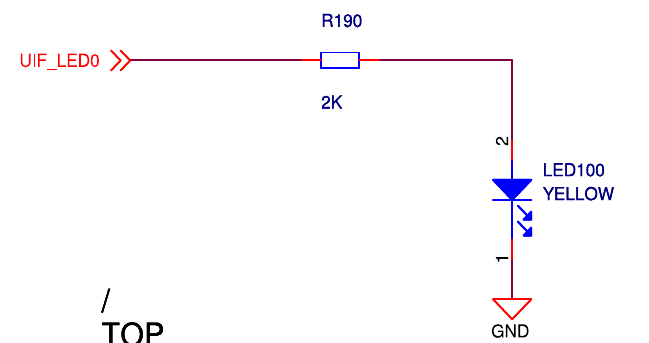
\includegraphics[width=0.85\textwidth, keepaspectratio]{imatges/led.png}
 \caption{Esquemàtic mostrant un LED connectat a un pin de GPIO}
 \label{fig:led}
\end{figure}

Existeixen diferents formes de configurar un pin segons el fabricant i la tecnologia, la més comuna és el mode {\em push-pull} que permet forçar un valor '1' o '0' segons convingui. Una altra opció que de vegades cal fer servir és el mode {\em open-drain}, que la sortida només pot forçar el valor '0' però no el valor '1'.

En aquest cas, per forçar el valor '1' es fa servir una resistència connectada a 3.3 volts; aquesta mena de resistència s'anomena un {\em \gls{pull-up}}. Aquesta mena de resistències (o el seu complementari, un {\em \gls{pull-down}}) també s'utilitza en la connexió de polsadors o botons, de manera que quan el botó no està polsat, la resistència de {\em pull-up} (o de {\em pull-down}) força el valor corresponent.

\begin{figure}
 \centering
 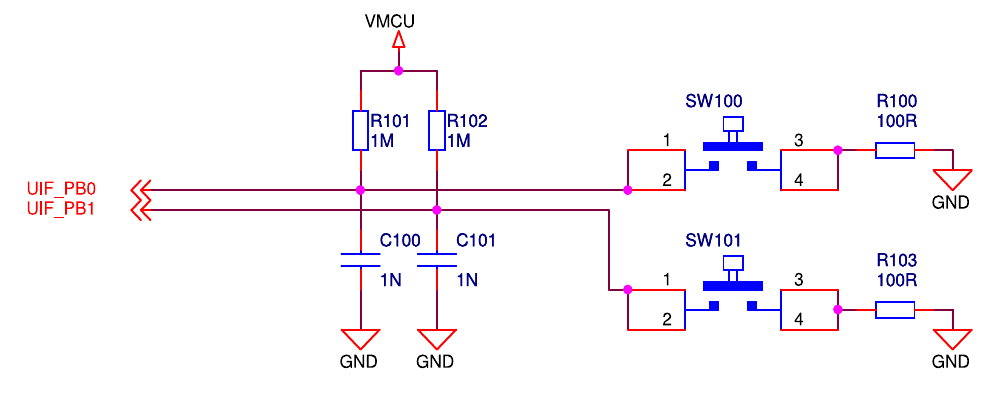
\includegraphics[width=0.85\textwidth, keepaspectratio]{imatges/buttons.png}
 \caption[Esquemàtic amb resistències de {\em pull-ups}]{Esquemàtic amb resistències de {\em pull-ups} (etiquetades com R101 i R102)}
 \label{fig:pullup}
\end{figure}

Com es veu al esquemàtic de la Figura~\ref{fig:pullup}, quan no es prem el botó les resistències etiquetades R101 i R102 fan que la línia estigui a ‘1' lògic ({\em pull-up}). En quan es prem el botó, aquest connecta GND a la línia i per tant passa a tenir el valor lògic ‘0'.

Cal saber també que la quantitat de corrent que un pin individual pot proporcionar està limitada i, en alguns casos, es pot seleccionar la quantitat màxima de corrent que pot donar un pin concret.

\section{Un exemple senzill}
\label{sub:GPIO_2_example}
Farem un codi que llegeixi l'estat dels botons de la placa, i en cas que estiguin pitjats, s'encén o apaga el LED. Veiem el codi el llistat~\ref{gpio_example}.

\begin{lstlisting}[style=customc,caption={Codi d'exemple de GPIO},label=gpio_example]
CMU_ClockEnable(cmuClock_GPIO, true);

GPIO_PinModeSet(gpioPortD,  7, gpioModePushPullDrive, 0); /* LED */
GPIO_PinModeSet(gpioPortD,  8, gpioModeInput, 0); /* Boto 0 */
GPIO_PinModeSet(gpioPortB, 11, gpioModeInput, 0); /* Boto 1 */

/* Infinite loop */
while (1) {
  if (GPIO_PinInGet(gpioPortD, 8) == 0) {
    GPIO_PinOutClear(gpioPortD, 7);
  }
  if (GPIO_PinInGet(gpioPortB, 11) == 0) {
    GPIO_PinOutSet(gpioPortD, 7);
  }
}
\end{lstlisting}

El primer que es fa amb la sentència {\bf CMU\_ClockEnable()}\index{CMU\_ClockEnable()} és alimentar amb un rellotge al perifèric \gls{GPIO}. En la arquitectura Cortex-M de Silicon Labs cal fer això per cada perifèric que fem servir. D'aquesta manera, un perifèric que no necessitem no rep cap rellotge i el seu consum és disminueix dràsticament.

Tot seguit es configuren els 3 pins que utilitzarem:
\begin{itemize}
 \item PD7 com sortida per controlar el LED,
 \item PD8 i PB11 com entrades connectades als botons 0 i 1.
\end{itemize}

Un cop configurats els pins, dins el bucle infinit es va mirant tota l'estona per {\em polling} el valor dels dos pins d'entrada i canviant el valor de sortida cap al LED segons toqui.


\section{BSP}
\label{sec:BSP}

Podem començar a introduir el concepte de \gls{BSP} que no són més que funcions específiques per la nostra PCB de manera que ens aïllen la implementació de la funcionalitat.

Anem a suposar que canviem de PCB (o de versió) i el LED que volem encendre ja no està connectat al pin D7 si no que està, posem per cas, al E2. Caldria canviar totes les crides que tinguéssim al nostre codi de l'estil vist al Llistat \ref{orig_gpio_bsp} per la del Llistat \ref{change_gpio_bsp} amb tots els errors que això provocar.

\begin{lstlisting}[style=customc, caption=Codi de configuració d'un pin, label=orig_gpio_bsp]
GPIO_PinOutSet(gpioPortD, 7);
\end{lstlisting}

\begin{lstlisting}[style=customc, label=change_gpio_bsp, caption=Codi amb la nova configuració del pin]
GPIO_PinOutSet(gpioPortE, 2);
\end{lstlisting}

Una forma molt habitual de treballar és escriure funcions amb les funcionalitats més comunes i que ens amaguin aquests detalls. Així, pel nostre exemple podríem definir les funcions del Llistat \ref{BSP_example}.
\index{LedInit()}\index{LedOn()}\index{LedOff()}\index{GPIO\_PinOutSet()}\index{GPIO\_PinModeSet()}\index{GPIO\_PinOutClear()}
\begin{lstlisting}[style=customc, label=BSP_example, caption=Exemple de BSP senzill]
LedInit() {
  GPIO_PinModeSet(gpioPortD, 7, gpioModePushPullDrive, 0); /* LED */
}

LedOn() {
  GPIO_PinOutSet(gpioPortD, 7);
}

LedOff() {
  GPIO_PinOutClear(gpioPortD, 7);
}
\end{lstlisting}

Fent servir aquestes funcions enlloc de les crides directes al GPIO ens permetran introduir canvis a la PCB sense haver de canviar gaire el nostre codi.

Habitualment en el BSP s'inclouen les inicialitzacions dels diversos rellotges (veure~{\fullref{sec:clocks}}), les funcions per accedir a recursos propis de la placa com LEDs o botons, configuració de les opcions de {\em Debug} (Veure~{\fullref{sub:console}}), etc.

\section{Manipulant bits individuals}
\label{sec:bits}

Tot i que no és específic dels GPIOs, veurem aquí com manipular bits individuals en C. Sovint ens caldrà posar a valor '0' o '1' un bit individual d'una variable sense canviar el valor de la resta dels bits, veiem aquí les receptes per fer-ho.

\begin{remark}
 La numeració de bits en C comença pel 0, així el bit menys significatiu d'una variable serà sempre el 0 i el més significatiu $N-1$, amb $N$ el nombre de bits de la variable. Per situar un 1 a un bit determinat, en C es fa servir l'operador {\bf <{}<}, que desplaça cap a l'esquerra el valor de l'esquerra tants bits com indiqui el valor de la dreta.
\end{remark}

L'exemple per aquesta secció es troba al repositori en el projecte \href{https://github.com/mariusmm/cursembedded/tree/master/Simplicity/Bit_1}{Bit\_1}.
\index{|}
\subsection{Posar a 1 un bit}
Per posar un bit concret a '1' d'una variable tant sols cal fer una OR lògica (símbol {\bf |}) tal com es veu al Llistat~\ref{example_bit}.

En aquest cas, primer es posa a '1' el bit 4 de la variable {\em my\_variable}.
\index{main()}
\begin{lstlisting}[style=customc, label=example_bit, caption=Manipulant un bit concret d'una variable]
void main(void) {
  ...
  uint8_t my_variable;
  ...
  my_variable = 5;
  // Set to '1' bit 4
  my_variable |= (1 << 4);
  printf("my_variable: 0x%02X\r\n", my_variable); // should be 0x15
  // Now set to '0' bit 2
  my_variable &= ~(1 << 2);
  printf("my_variable: 0x%02X\r\n", my_variable); // should be 0x11
  // Now we toggle bit 0 twice
  my_variable ^= (1 << 0);
  printf("my_variable: 0x%02X\r\n", my_variable); // should be 0x10
  my_variable ^= (1 << 0);
  printf("my_variable: 0x%02X\r\n", my_variable); // should be 0x11
  ...
  
  if ( (my_variable & 0x10) != 0 ) {
    /* the variable my_variable has the 4th bit set */
  }
}
\end{lstlisting}

\index{\&}\index{\~{}}
\subsection{Posar a 0 un bit}
Per posar a zero un bit individual, la feina a fer és una mica més estranya, ja que cal fer una AND lògica amb tots els bits a '1' menys el desitjat que haurà d'estar a '0'. Això es pot fer amb la mateixa construcció d'abans i fent l'operació NOT bit a bit (amb el símbol {\bf \~{}}) abans de fer la AND (símbol {\bf \&}).

En el mateix exemple es veu com, després de posar a 1 el bit 4, es posa a 0 el bit 3 amb la operació AND comentada.

\index{\^{}}
\subsection{{\em Toggle} un bit}
Per a fer un {\em toggle} d'un bit individual, el que cal fer és la operació lògica XOR (símbol {\bf \^{}}) amb el bit desitjat al valor '1'.

A l'exemple es fa {\em toggle} dues vegades al bit 0 de la variable.

\subsection{Comparar si un bit està a cert valor}
L'altre necessitat que apareix sovint és la de comprovar el valor d'un bit determinat d'una variable.

L'opció més habitual és fer una AND lògica entre la variable i el bit interessant i comprovar que el resultat és diferent de '0'. Si la comparació dona cert vol dir que el bit en qüestió està a '1', en cas contrari, el bit d'interès té el valor '0'. Es pot veure al final de l'exemple al Llistat~\ref{example_bit}, on es comprova que el bit 4 de la variable sigui valgui '1'.

\begin{remark}
Aquesta mena d'operacions són força propicies per introduir {\em bugs} complicats de detectar. Operar per error un bit que no pertany a aquella mida de variable pot portar a errors molt difícils de detectar i el compilador no donarà cap mena de error o avís.
\end{remark}


\chapter{Controlador d'interrupcions}
\label{ch:IRQ}
Una interrupció (\gls{IRQ}) és un succés que interromp l'execució normal del processador i passa a executar un codi de programa especial pel succés concret. La \gls{ISR} és el codi que es crida per a cada succés o interrupció.

Cada interrupció té assignada una ISR pròpia. Aquesta informació s'acostuma a guardar en una zona de memòria especial, anomenada memòria de vectors d'interrupció.

Les IRQs estan enumerades i tenen prioritats, així habitualment, un valor menor vol dir major prioritat. Aquest valor de IRQ també es fa servir per saber quina posició dels vectors d'interrupció es troba la ISR corresponent.

El controlador d'interrupcions gestiona quines interrupcions rebudes arriben al processador, segons les prioritats i si la interrupció concreta està activada o no.

Veurem un cas amb els GPIO, el codi està disponible \href{https://github.com/mariusmm/cursembedded/tree/master/Simplicity/GPIO_2}{al repositori}. En aquest cas, el que es fa primer és configurar els pins perquè generin una interrupció HW al flanc de baixada (recordem el {\em pull-up} a la PCB, Figura~\ref{fig:pullup}). Tot seguit s'activen les interrupcions corresponents.
\index{NVIC\_EnableIRQ()}\index{GPIO\_IntConfig()}
\begin{lstlisting}[style=customc]
 /* Set Interrupt configuration for both buttons */
GPIO_IntConfig(gpioPortD, 8, false, true, true);
GPIO_IntConfig(gpioPortB, 11, false, true, true);

/* Enable interrupts */
NVIC_EnableIRQ(GPIO_EVEN_IRQn);
NVIC_EnableIRQ(GPIO_ODD_IRQn);
\end{lstlisting}

En el cas dels Cortex-M de SiliconLabs, els pins de \gls{GPIO} poden generar només 2 interrupcions, els pins parells la interrupció GPIO\_EVEN\_IRQ i els pins senars la GPIO\_ODD\_IRQ \cite[405]{EFM32GRM}. En els microcontroladors de ST, hi ha una arquitectura diferent i cada pin d'entrada pot generar una IRQ segons el seu índex de manera que el pin PA2, el PB2, el PC2 etc. generen la IRQ EXTI2, però només un d'aquests pins pot generar la IRQ \cite[384]{STM32F4RM}.

En el cos de l'exemple, com que els botons estan connectats al pin D8 i B11 cada un d'ells activarà una de les dues interrupcions.

La \gls{ISR} per la interrupció parell la veiem al Llistat~\ref{gpio_isr}.
\index{GPIO\_EVEN\_IRQHandler()}\index{GPIO\_IntClear()}\index{GPIO\_IntGet()}\index{GPIO\_PinOutClear()}
\begin{lstlisting}[style=customc, label=gpio_isr, caption=Exemple d'ISR per GPIO]
void GPIO_EVEN_IRQHandler(void) {
  uint32_t aux;

  aux = GPIO_IntGet();

  /* clear flags */
  GPIO_IntClear(aux);

  /* Set LED off */
  GPIO_PinOutClear(gpioPortD, 7);
}
\end{lstlisting}

A l'arquitectura Cortex-M el nom de les ISR està fixat en un fitxer de l'entorn de programació, de manera que només cal escriure una funció amb el nom correcte i ja tenim definida la ISR. El fitxer que defineix les ISR depèn de cada model de microcontrolador, en el nostre cas és el fitxer startup\_efm32tg.S.

En el cas de l'arquitectura Cortex, la pròpia ISR ha de netejar el \gls{flag} d'interrupció que l'ha cridat. Això es fa al principi de tot de la \gls{ISR}, llegint quins \glspl{flag} estan actius (funció {\bf GPIO\_IntGet()}\index{GPIO\_IntGet()}) i tot seguit netejant aquests mateixos \glspl{flag} ({\bf GPIO\_IntClear()}\index{GPIO\_IntClear()}).

A continuació, s'encén o s'apaga el LED segons correspongui (a una ISR s'apaga, a l'altre s'encén).

L'altre cosa a destacar d'aquest exemple és el que hi ha dins el bucle infinit, que està buit. I està buit perquè, en aquest exemple, el microcontrolador no té res a fer fins que no hi hagi una interrupció provinent d'un botó.

En una aplicació real, en aquest bucle es podrà posar codi que si s'hagi d'executar contínuament, o instruccions que posin “a dormir” el microcontrolador tot esperant una interrupció, etc. Tot això ho anirem veient més endavant.

\section{Escrivint ISRs en C}
\label{sec:IRQ_example}
Com ja sabem, les \gls{ISR} són les funcions especials que s'executen tant bon punt es dispara una interrupció determinada.

Tradicionalment les adreces a aquestes \glspl{ISR} (anomenats de vegades vectors d'interrupció) s'emmagatzemaven a una zona especial de la memòria del processador. Quan el processador rebia una \gls{IRQ}, com que aquestes van numerades simplement calcula l'offset de la IRQ a la taula de ISRs i executa aquella funció determinada.

En els ARM Cortex amb els que treballem això es fa tal qual acabem d'explicar. En el cas dels Cortex (i la majoria de microcontroladors i processadors) la taula de vectors d'interrupcions es col·loca a partir de la posició 0 de memòria.

El que cal, doncs, és que les nostres eines de compilació posin aquests vectors com toca a cada un dels binaris que generem. En el cas de les eines per Cortex (tant Simplicity com les eines de ST ho fan així), aprofiten un codi d'inicialització proporcionat per ARM anomenat, en el nostre cas startup\_efm32tg.S. Aquest fitxer està escrit en assemblador i, entre d'altres coses, té el codi que es veu a la Figura~\ref{fig:ISR}:

\begin{figure}
 \centering
 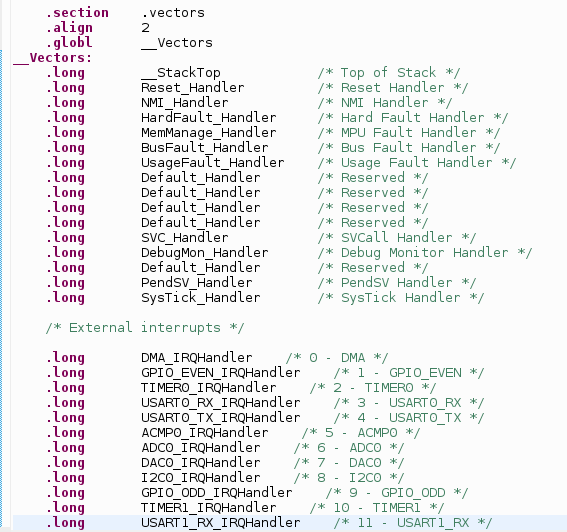
\includegraphics[width=0.85\textwidth, keepaspectratio]{imatges/interruptvectorcortex.png}
 \caption{Vectors d'interrupció}
 \label{fig:ISR}
\end{figure}

Com es pot veure, aquest codi declara el nom de les ISRs corresponents a cada una de les IRQs possibles al microcontrolador. Més endavant en el mateix fitxer, es posa una funció per defecte per a cada una de les ISR que és només un bucle sense fi. Com que aquesta funció es declara com {\em weak}, nosaltres podrem sobreescriure–la en cas que ho vulguem fer.

En el cas de Cortex, les funcions de ISR no han de ser definides de cap forma especial, més enllà de posar el nom que li correspongui.

En altres arquitectures, com ara AVR d'Atmel, les ISR han de retornar d'una manera diferent a les funcions normals donat que durant la crida a una ISR no es guarden tots els registres com es fa a una crida a una funció normal. Si escrivim la funció en assemblador, enlloc d'una instrucció {\bf RET} ens caldrà escriure una instrucció {\bf RETI}.

Si estem treballant en llenguatge C, com que el compilador posa una instrucció {\bf RET} quan acaba la funció, caldrà indicar-li d'alguna forma que la funció en qüestió és una ISR i que ha d'acabar-la amb una instrucció {\bf RETI}.

Això, en el cas d'AVR es fa com es veu al Llistat \ref{ISR_AVR_1} o \ref{ISR_AVR_2} depenent del tipus de compilador que estiguem fent servir.

\begin{lstlisting}[style=customc, label=ISR_AVR_1, caption=Exemple d'ISR per AVR]
#pragma vector=TIMER0_OVF_vect
__interrupt void MotorPWMBottom() {
  // codi
}
\end{lstlisting}

\begin{lstlisting}[style=customc, label=ISR_AVR_2, caption=Exemple d'ISR per AVR]
ISR(PCINT1_vect) {
  //codi
}
\end{lstlisting}


\section{Fent servir ISRs}
Com ja hem comentat, una \gls{ISR} s'executa quan es dispara una \gls{IRQ}. Durant l'execució de la ISR el microcontrolador està en un mode d'execució especial, amb les demés IRQs desactivades (depèn de l'arquitectura això pot no ser així).

Donat que la resta d'IRQs poden estar desactivades, és important que el temps que el processador estigui executant una ISR sigui el mínim possible i que el codi, per tant, sigui el més senzill possible.

Si el que hem de fer, a part de tasques molt simples a la ISR, és engegar o controlar un procés més complicat, aquest procés no el farem dins la ISR, si no en un procés a part i comunicarem via \glspl{flag}, cues, semàfors o mecanismes similars la ISR amb el procés. Així minimitzem el temps que el processador està en mode ISR.

\subsection{Ús de variables globals}
\label{sb:volatile}
Com ja hem vist breument a \fullref{sub:memory-mapped} hi ha una paraula reservada que es fa servir quan es fan accessos a memòria i altres usos d'una variable on el compilador no ha d'actuar amb cap optimització. La paraula reservada {\bf volatile} davant la declaració d'una variable indica al compilador que la variable s'hi ha d'accedir tal com diu el codi i no efectuar cap optimització.

\begin{remark}
En el cas de modificar el valor d'una variable global des d'una ISR, cal declar-la com a {\bf volatile}.
\end{remark}

\chapter{Timers}
\label{sub:Timers}
Un {\em \gls{Timer}} (temporitzador) és un dels perifèrics més habituals de trobar en un microcontrolador. Bàsicament consisteix en un comptador que pot generar alguna interrupció quan arriba a un cert llindar o al seu valor límit. Com sempre, cada fabricant el fa segons el seu criteri i, per tant, cada un té característiques diferents.

Normalment els {\em timers} es poden connectar a diferents rellotges disponibles dins el microcontrolador. A més, força sovint els {\em timers} poden dividir prèviament la freqüència del rellotge que l'alimenta per reduir-la encara més. Així, podem tenir un rellotge d'1 MHz alimentant un {\em timer} que abans de que hi entri es divideixi per 8 per tenir un rellotge efectiu de 125 kHz. Amb això, si configurem el {\em timer} perquè compti fins al valor 125000, tindrem que el {\em timer} generarà una interrupció cada segon.

En el cas de Silicon Labs, els Timers tenen múltiples opcions \cite[249]{EFM32GRM}:

\begin{itemize}
 \item comptador de 16 bits
 \item pre-escalatge del rellotge: el rellotge d'entrada es pot pre-escalar (dividir) per diversos factors (de 2 fins a 1024).
 \item diverses fonts de rellotge
 \item diverses formes de comptatge (cap a munt, cap avall, amunt i avall, etc.)
 \item 3 canals per Timer, per generar diverses interrupcions (per {\em overflow}, per arribar a un llindar, {\em underflow}, etc.)
\end{itemize}



Tot plegat fa que sigui força complicat de configurar, i com ve sent costum, el fabricant ens dona una biblioteca per simplificar-nos una mica la vida.

Els controls que tenim habitualment per un Timer, un cop configurat, són \cite{EMLIB}:

\begin{itemize}
 \item engegar i parar el Timer ({\bf TIMER\_Enable()}\index{TIMER\_Enable()} a EMLIB).
 \item llegir o configurar el màxim valor pel timer ({\bf TIMER\_TopGet()}\index{TIMER\_TopGet()} / {\bf TIMER\_TopSet()}\index{TIMER\_TopSet()} a EMLIB).
 \item llegir o configurar el valor pel compare ({\bf TIMER\_CompareGet()}\index{TIMER\_CompareGet()} / {\bf TIMER\_CompareSet()}\index{TIMER\_CompareSet()} a EMLIB).
\end{itemize}

Els usos que li podem donar a aquest perifèric són variats, els més habituals són els següents::
\begin{itemize}
 \item Comptar el temps: es configura per a que generi una interrupció cada segon i ja tenim un rellotge de temps real. Hi ha perifèrics específics per aquesta tasca (\glspl{RTC}) com es veurà a \fullref{sub:RTC}.
 \item Fer {\em delays} acurats: de vegades cal que un senyal o una acció passi després d'un cert temps. Amb un Timer ben configurat podem comptar temps petits de l'ordre de microsegons.
 \item Comptar polsos externes: segons quins Timers poden comptar segons una entrada externa, i aquesta no cal que sigui un rellotge. Pot ser, per exemple, les pulsacions d'un botó o les transicions d'un senyal.
 \item Generar senyals \gls{PWM}: tipus de senyal digital per controlar motors o d'altres dispositius (Veure~{\fullref{sub:PWM}}).
\end{itemize}

\section{Exemple senzill amb un Timer}
\label{sub:Timers_exemple}
El \href{https://github.com/mariusmm/cursembedded/tree/master/Simplicity/Timer_1}{primer exemple} fa servir un Timer per esperar-se 1 segon a canviar d'estat el LED (fer un {\em toggle}) després que es premi el Botó 0.

El que es fa en primer lloc és configurar el Timer0 amb un seguit d'opcions. Les més importants de cara a l'exemple són:
\begin{itemize}
 \item .prescale = timerPrescale1024 que configura el divisor de rellotge a 1024.
 \item .mode = timerModeUp així el Timer només compta cap amunt.
 \item .oneShot = true en aquest cas, un cop arribi al màxim valor el Timer es pararà.
\end{itemize}

Un cop configurat el Timer, s'entra en el bucle infinit.
Dins el bucle infinit, si es polsa el botó 0, es posa el comptador del Timer a 0 i s'engega el comptador (Llistat~\ref{Timer_example_1}).
\index{TIMER\_CounterSet()}\index{TIMER\_Enable()}\index{main()}\index{GPIO\_PinInGet()}
\begin{lstlisting}[style=customc, label=Timer_example_1, caption=Codi d'exemple d'ús d'un Timer ]
void main(void) {
  ...
  if (GPIO_PinInGet(gpioPortD, 8) == 0) {
    TIMER_CounterSet(TIMER0, 0);
    TIMER_Enable(TIMER0, true);
  }
}
\end{lstlisting}

Tot seguit, es comprova si el comptador ha arribat al valor {\bf TOP\_VALUE} usant la funció {\bf TIMER\_CounterGet()}\index{TIMER\_CounterGet()}, si és així es fa {\em toggle} del LED (s'encén si estava apagat o el contrari), s'atura el Timer i es posa el seu comptador a 0 (Llistat~\ref{Timer_example_2}).

\index{main()}\index{TIMER\_CounterGet()}\index{TIMER\_Enable()}\index{TIMER\_CounterSet()}\index{GPIO\_PinOutToggle()}
\begin{lstlisting}[style=customc, label=Timer_example_2, caption=Codi per comprovar si el Timer ha arribat a cert valor]
void main(void) {
  ...
  /* If timer count gets to TOP_VALUE, toggle LED and stop Timer */
  if (TIMER_CounterGet(TIMER0) >= TOP_VALUE) {
    GPIO_PinOutToggle(gpioPortD, 7);
    TIMER_Enable(TIMER0, false);
    TIMER_CounterSet(TIMER0, 0);
  }
  ...
}
\end{lstlisting}

Com hem calculat el valor {\bf TOP\_VALUE} (13671)?

\begin{verbatim}
Rellotge d'entrada al Timer: 14.000.000 Hz (14 MHz)
Prescaler: 1024 (Seleccionat al inicialitzar el timer)
Freqüència de treball del Timer = 14.000.000 / 1024 = 13.671,875 Hz
\end{verbatim}

Per tant, en un segon el comptador del Timer haurà comptat fins a 13.671 (o 13.672, no ve d'un tick!).

En aquest exemple hem fet servir el Timer d'una forma força rudimentària, ja que no és gaire habitual fer {\em polling} d'un Timer per transcorre un temps determinat. Es fa servir aquest mètode per implementar funcions tipus {\bf Delay()} simples. A continuació veurem un exemple més complicat basat en interrupcions.

\section{Exemple més complex amb el Timer}
\label{sub:Timers_exemple_2}
Al \href{https://github.com/mariusmm/cursembedded/tree/master/Simplicity/Timer_2}{segon exemple} fem servir interrupcions
per obtenir informació del Timer i així alliberar la CPU.

Primer de tot, cal saber per quines condicions pot generar interrupcions el nostre Timer. En el cas de la família EFM32, cada Timer té només una interrupció (anomenada TIMERn\_IRQn) però tenen els següents esdeveniments que poden generar una interrupció \cite{EFM32GRM}:

\begin{itemize}
 \item {\em Overflow}: quan el comptador arriba a {\bf TOP}
 \item {\em Underflow}: quan el comptador arriba a 0
 \item {\em Compare Match}: quan el comptador arriba a un valor determinat. N'hi ha un per cada canal del Timer.
\end{itemize}

Així doncs, quan estiguem a la \gls{ISR} del Timer si hem activat més d'un esdeveniments a que generi la interrupció haurem de mirar quin esdeveniments ha estat.

El Timer es configura igual que a l'exemple anterior, i a més s'activen les interrupcions per aquest perifèric amb el codi que es veu a \ref{Timer_enableIRQ}.
\index{TIMER\_IntEnable()}\index{NVIC\_EnableIRQ()}
\begin{lstlisting}[style=customc, label=Timer_enableIRQ, caption=Codi corresponent a l'activació de les IRQs del Timer]
 /* Enable overflow interrupt */
TIMER_IntEnable(TIMER0, TIMER_IF_OF);

/* Enable IRQ for Timer 0*/
NVIC_EnableIRQ(TIMER0_IRQn);
\end{lstlisting}

Amb això, un cop s'engegui el Timer i quan arribi el comptador a {\bf TOP} llençarà la interrupció {\bf TIMER0\_IRQn}, que executarà la {\bf ISR TIMER0\_IRQHandler()}\index{TIMER0\_IRQHandler()} que es veu al Llistat~\ref{Timer_IRQ} on simplement es netegen els \glspl{flag} d'interrupció i es fa {\em toggle} del \gls{LED}.
\index{TIMER\_IntGet()}\index{TIMER\_IntClear()}
\begin{lstlisting}[style=customc, label=Timer_IRQ, caption=ISR del Timer]
void TIMER0_IRQHandler(void) {
  uint32_t flags;

  /* Clear flag for TIMER0 */
  flags = TIMER_IntGet(TIMER0);
  TIMER_IntClear(TIMER0, flags);

  /* Toggle LED ON/OFF */
  GPIO_PinOutToggle(gpioPortD, 7);
}
\end{lstlisting}

La configuració i la posada en marxa del Timer es fa a la \gls{ISR} del botó 0, de manera similar a com ja havíem fet anteriorment a d'altres exemples: primer es netegen els {\em flags} de la \gls{IRQ}, tot seguit es posa el comptador del Timer a 0, es posa el valor màxim i per últim s'engega el Timer (Llistat~\ref{GPIO_ISR_Timer}).

\index{GPIO\_EVEN\_IRQHandler()}\index{GPIO\_IntGet()}\index{GPIO\_IntClear()}
\index{TIMER\_CounterSet()}\index{TIMER\_TopSet()}\index{TIMER\_Enable()}
\begin{lstlisting}[style=customc, label=GPIO_ISR_Timer, caption=ISR del GPIO per l'exemple del Timer]
void GPIO_EVEN_IRQHandler(void) {
  uint32_t flags;

  /* clear flags */
  flags = GPIO_IntGet();
  GPIO_IntClear(flags);

  /* Set counter to 0  */
  TIMER_CounterSet(TIMER0, 0);

  /* Set TIMER Top value */
  TIMER_TopSet(TIMER0, TOP_VALUE);

  /* Start Timer */
  TIMER_Enable(TIMER0, true);
}
\end{lstlisting}

Per últim, fer notar que al bucle infinit final del {\bf main()}\index{main()} no hi ha cap codi, ja que la \gls{CPU} no té res a fer mentre espera la pulsació del botó o que s'exhaureixi el temps, En el tema de baix consum (\fullref{ch:low-power}) es veurà com aprofitar aquest fet per reduir el consum del sistema amb un exemple a \fullref{sub:letimer_example}.

Al diagrama de seqüència de  la Figura~\ref{fig:TImer_2seq} explica l'exemple.

\begin{figure}
 \centering
 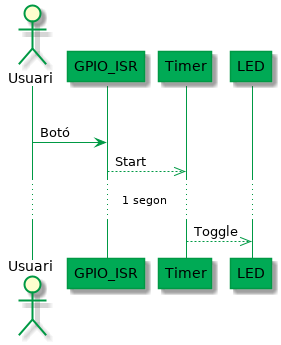
\includegraphics[width=0.65\textwidth, keepaspectratio]{imatges/Timer2Seq.png}
 \caption{Diagrama de seqüència de l'exemple Timer\_2}
 \label{fig:TImer_2seq}
\end{figure}

\chapter{RTC}
\label{sub:RTC}

Un altre perifèric que acostumem a trobar als microcontroladors actuals és una mena de \gls{Timer} una mica especial. Habitualment aquests perifèrics serveixen per tenir un control de temps en segons i/o un calendari, enlloc de temps molts més curts de mil·lisegons o microsegons com els Timers que ja hem vist.

Aquest tipus de perifèrics acostumen a fer servir una entrada de rellotge pròpia de 32,768 kHz (32.768 Hz), que és una freqüència de rellotge molt habitual per aquestes feines. Algunes famílies de microcontroladors poden funcionar amb altres freqüències o generar-la internament per fer el sistema més senzill.

Els RTC varien força de fabricant a fabricant, així els STM32 tenen un RTC complet, on podem guardar dia, mes i any, hora minut i segons i el dispositiu mateix manté la data (dies del mes, anys de traspàs, etc.), fent molt senzill mantenir una data dins el dispositiu (veure Figura~\ref{fig:STRTC}) \cite[799]{STM32F4RM}.

\begin{figure}
 \centering
 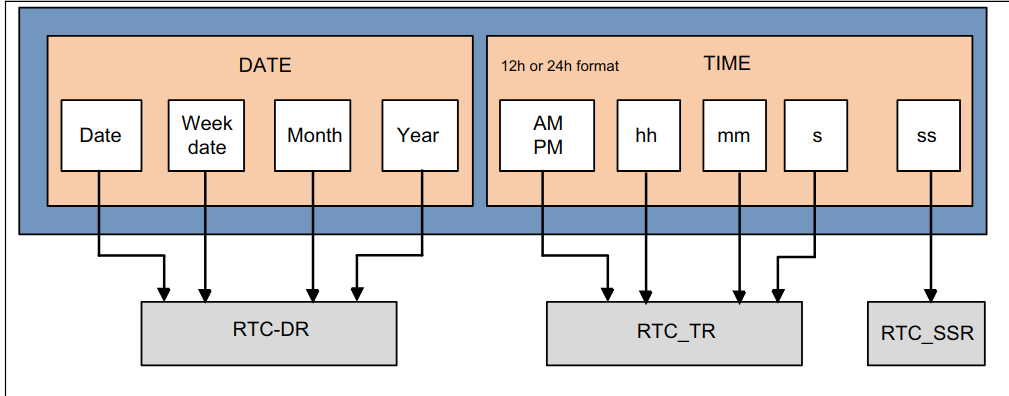
\includegraphics[width=0.85\textwidth, keepaspectratio]{imatges/RTC_STM32.png}
 \caption{Registres del RTC de STM32 \cite{ST_AN3371}}
 \label{fig:STRTC}
\end{figure}

Per contra, els RTCs de EFM32 són força més senzills, i és, de fet, un Timer de 24 bits de molt baix consum amb una entrada de rellotge pròpia i que es pot triar cada quan generen una interrupció \cite[285]{EFM32GRM}. Si triem fer una interrupció cada segon, podem manegar per SW la gestió de l'hora i el calendari.

\href{https://github.com/mariusmm/cursembedded/tree/master/Simplicity/RTC}{A l'exemple per EFM32} tant sols se selecciona el rellotge de 32 kHz extern (LFXO), el divisor a 32768 per tenir un tic cada segon i es configura per a que generi una interrupció cada 2 segons (veure Llistat~\ref{RTCInit}). En aquest exemple, a la \gls{ISR} només es canvia el LED (s'apaga o encén segons el seu estat actual) (veure Llistat~\ref{RTCISR}).

\index{CMU\_ClockSelectSet()}\index{CMU\_ClockDivSet()}\index{NVIC\_EnableIRQ()}
\index{RTC\_CompareSet()}\index{RTC\_IntEnable()}\index{NVIC\_ClearPendingIRQ()}
\begin{lstlisting}[style=customc, caption={Inicialització del RTC}, label=RTCInit]
void main(void) {
  ...
  CMU_ClockSelectSet( cmuClock_LFA, cmuSelect_LFXO );
  CMU_ClockDivSet( cmuClock_RTC, cmuClkDiv_32768 );
  ...

  RTC_CompareSet(0, 2);

  /* Enabling Interrupt from RTC */
  RTC_IntEnable(RTC_IFC_COMP0);
  NVIC_ClearPendingIRQ(RTC_IRQn);
  NVIC_EnableIRQ(RTC_IRQn);
  ...
}
\end{lstlisting}

\index{RTC\_IRQHandler()}\index{RTC\_IntClear()}\index{GPIO\_PinOutToggle()}
\begin{lstlisting}[style=customc,caption={ISR del RTC},label=RTCISR]
void RTC_IRQHandler(void) {
  /* Clear interrupt source */
  RTC_IntClear(RTC_IFC_COMP0);

  GPIO_PinOutToggle(gpioPortD, 7);
}
\end{lstlisting}


Si volguéssim mantenir un rellotge fent servir aquest perifèric podríem configurar-lo perquè generi una interrupció cada segon, i dins la \gls{ISR} mantenir un comptador de segons i actualitzar la data segons això.

\section{RTC externs}
Quan la majoria de microcontroladors no incloïen un RTC intern com els que hem vist, era habitual fer servir un dispositiu \gls{RTC} extern. D'aquests dispositius n'hi ha de tota mena però la majoria tenen les següents característiques:

\begin{itemize}
 \item Interface \gls{I2C} (veure \fullref{sub:I2C}) amb el microcontrolador.
 \item Necessita un cristall de 32.768 Hz.
 \item Un error d'aproximadament un segon a l'any.
 \item Actualitza data i hora, calculant anys de traspàs.
 \item Capacitat de generar interrupcions segons una alarma programable.
 \item Molt baix consum i alimentació separada amb bateria (pila botó).
 \item Molts d'ells tenen una petita memòria RAM adreçable per guardar-hi dades persistents.
\end{itemize}

Amb aquesta mena de dispositiu, el microcontrolador es descarrega de gestionar el calendari i només cal accedir als registres del RTC extern per saber l'hora o data del sistema. A la majoria dels casos també és possible programar alguna mena d'alarma, de forma que quan arriba cert temps o data una línia dedicada pot generar una interrupció al microcontrolador. Alguns models també tenen la possibilitat de generar un senyal de forma periòdica per tenir, per exemple, un senyal a 128 Hz.

Habitualment l'alimentació d'aquests dispositius es pot fer per un canal separat de l'alimentació principal i usant una bateria o pila tipus botó. Això permet que el RTC sempre estigui alimentat encara que es perdi l'alimentació principal (per avaria, tall de corrent, canvi de bateries, etc.). Aprofitant que sempre tenen alimentació, força RTCs tenen una zona de memòria RAM per a que el microcontrolador pugui guardar-hi dades persistents. L'accés a aquesta zona de memòria també es fa mitjançant el bus \gls{I2C}, sent molt senzill emmagatzemar-hi dades.

Per últim, cal dir que són dispositius força barats (entre 0.5 € i 3 € per unitat en volums petits), sent una bona opció en cas que el nostre microcontrolador no disposi d'aquesta funcionalitat \cite{RTCDS1}\cite{RTCDS2}\cite{RTCDS3}.

\chapter{PWM}
\label{sub:PWM}
El \gls{PWM} és una tècnica per aconseguir controlar la potència subministrada a un dispositiu mitjançant un senyal digital. Simplificant, fent que un senyal digital (‘1' o ‘0') estigui més o menys estona a ‘1' aconseguim controlar la potència que rep el dispositiu a la sortida.

Aquest tipus de modulació es fa servir per controlar motors simples (motors DC) on enlloc d'enviar un voltatge variable per controlar la velocitat enviem un senyal PWM. Així, si enviem polsos més llargs el motor girarà més ràpid i si enviem polsos més curts el motor girarà més a poc a poc. Com que el voltatge que se li envia sempre es el màxim, la potència del motor és sempre la màxima.

Els dos paràmetres principals d'un senyal PWM són la seva freqüència i el seu \gls{duty cycle} (la durada del pols a ‘1' respecte la durada del pols a ‘0').

\href{https://github.com/mariusmm/cursembedded/tree/master/Simplicity/PWM_1}{A l'exemple} es fa servir el LED de la placa enlloc d'un motor. Posarem una freqüència molt petita, així la podrem veure amb els nostres ulls, i anirem canviant el \gls{duty cycle} amb els dos botons, de manera que podem veure què està passant.

Primer veiem què passa i després veiem com ho fa el codi.

Només programar la placa veiem el LED fent pampallugues força ràpid tota l'estona. Si polsem el botó 1 veurem que el LED va més ràpid, si tornem a polsar el botó 1 encara va més ràpid així fins que al cinquè cop que el polsem el LED es queda encès tota l'estona.

El que estem veient és que el LED va rebent un senyal PWM on el duty cycle cada cop és més gran (més estona encès que apagat) fins que al final és del 100\% (sempre encès). El ritme al que fa pampallugues el LED és (més o menys) la freqüència del PWM, que en aquest exemple és de 13.5~Hz.

\section{Generar PWM}
\label{sub:PWM_example}

La majoria de microcontroladors actuals tenen algun dispositiu HW que permet generar \gls{PWM}. En el cas dels micros de Silicon Labs, el dispositiu que ens permet generar-ne són els \glspl{Timer}.

Un Timer (veure la secció~\fullref{sub:Timers}) no és més que un comptador HW que genera interrupcions o sortides quan el comptador arriba a uns certs valors.

Per generar PWM, el Timer es configura el seu registre {\bf TOP} per a que ens doni la freqüència de funcionament del PWM desitjada. El que farà el Timer és comptar sempre fins a TOP i re-iniciar-se en quan hi arribi. Per generar el \gls{duty cycle} el que es fa es posar el valor desitjat al registre {\bf COMPARE} ({\bf CC}). El que farà el Timer és treure un ‘1' mentre el comptador no arribi a {\bf CC}, llavors posarà un ‘0' a la sortida fins que el comptador arribi a {\bf TOP}, on tornarà a començar el cicle (Figura~\ref{fig:pwm_timer})..

\begin{figure}
 \centering
 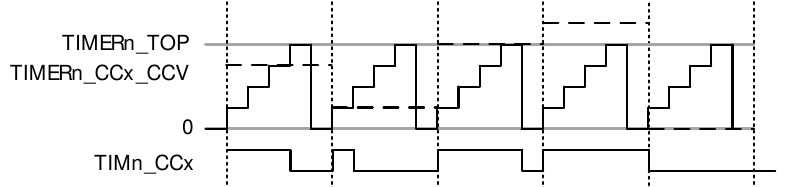
\includegraphics[width=0.85\textwidth, keepaspectratio]{imatges/pwm_timer.png}
 \caption{Generació de PWM amb un timer \cite[262]{EFM32GRM}}
 \label{fig:pwm_timer}
\end{figure}
En el codi d'exemple (Llistat \ref{Set_Timer_PWM}), el que es fa és configurar el TIMER1 en mode PWM i connectar la sortida del Timer al Pin D7 que és on està el LED connectat.

\index{TIMER\_InitCC()}
\begin{lstlisting}[style=customc, label=Set_Timer_PWM, caption=Configuració del Timer per l'exemple PWM]
 /* Set Timer */
TIMER_InitCC(TIMER1, 1, &timerCCInit);
TIMER1->ROUTE |= (TIMER_ROUTE_CC1PEN | TIMER_ROUTE_LOCATION_LOC4);
\end{lstlisting}

A continuació és configuren els dos registres importants per generar PWM (Llistat~\ref {Timer_PWM_Conf}). Com que volem una freqüència baixa pel \gls{PWM} per poder veure'l amb els nostres ulls, al registre {\bf TOP} hi posem {\bf PWM\_FREQ} (4000), que el calculem de la següent manera \cite{EFM32GRM}.
\begin{displaymath}
\text{Freq. de PWM} = \frac{\text{Freq Clk}}{\text{prescaler} * \text{valor TOP}} = \frac{14.000.000 \text{ Hz}}{256 * (4000 +1 )} = 13.67 \text{ Hz}
\end{displaymath}

\index{TIMER\_TopSet()}\index{TIMER\_CompareBufSet()}
\begin{lstlisting}[style=customc, label=Timer_PWM_Conf, caption=Configuració del Timer per l'exemple PWM]
TIMER_TopSet(TIMER1, PWM_FREQ);
TIMER_CompareBufSet(TIMER1, 1, pwm_value);
\end{lstlisting}

La resta del codi és senzill: es preparen les dues interrupcions per cada un dels botons, i quan algun dels dos es prem, la \gls{ISR} modifica el valor del registre {\bf CC} del Timer (un botó augmenta el duty cycle, l'altre el disminueix).

Si veiem el senyal generat amb un oscil·loscopi veiem el que es mostra a la Figura~\ref{fig:DutyCycle1} (estat per defecte).
\begin{figure}
 \centering
 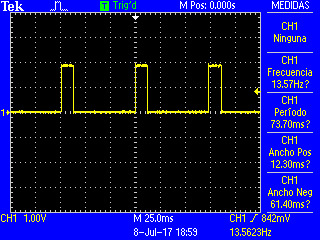
\includegraphics[width=0.85\textwidth, keepaspectratio]{imatges/DutyCycle1.png}
 \caption{PWM amb Duty Cycle al 16\%}
 \label{fig:DutyCycle1}
\end{figure}

Veiem que la freqüència real del senyal és de 13.57 Hz (73.70 ms de període) i que el senyal està a ‘1' 12.30 ms i a ‘0' a 61.40 ms.

Segons anem pitjant el botó 1 i anem augmentant el \gls{duty cycle} anem veient com està més estona a '1' el senyal (Figures~\ref{fig:DutyCycle2},
\ref{fig:DutyCycle3} i \ref{fig:DutyCycle4}).
Cal fixar-se que la freqüència no varia, sempre és \~13.5 Hz i el que va variant és l'estona que està a ‘0' o a ‘1' el senyal.

\begin{figure}
 \centering
 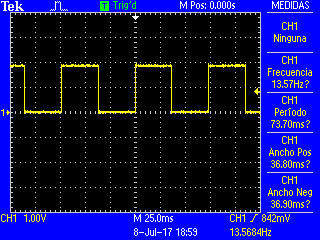
\includegraphics[width=0.85\textwidth, keepaspectratio]{imatges/DutyCycle2.png}
 \caption{PWM amb Duty Cycle al 50\%}
 \label{fig:DutyCycle2}
\end{figure}

\begin{figure}
 \centering
 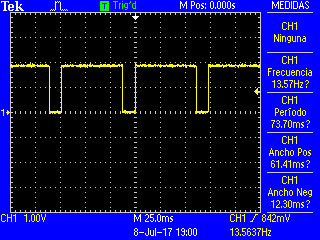
\includegraphics[width=0.85\textwidth, keepaspectratio]{imatges/DutyCycle3.png}
 \caption{PWM amb Duty Cycle al 83.3\%}
 \label{fig:DutyCycle3}
\end{figure}

\begin{figure}
 \centering
 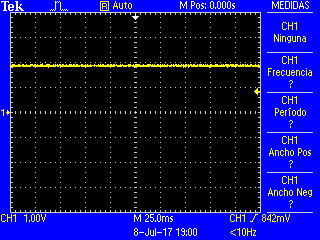
\includegraphics[width=0.85\textwidth, keepaspectratio]{imatges/DutyCycle4.png}
 \caption{PWM amb Duty Cycle al 100\%}
 \label{fig:DutyCycle4}
\end{figure}

Per acabar, es pot provar de canviar la freqüència del \gls{PWM} per a que no es vegi el LED fent pampallugues. Cal augmentar la freqüència a un valor que superi els 100Hz i enlloc de veure el LED encendre's i apagar-se, es veurà com varia la intensitat amb la que llueix.


\section{Controlant un servomotor}
Un servomotor és un dispositiu electromecànic de control senzill. La majoria d'ells son rotatius i permeten controlar l'angle d'actuació del motor amb un senyal digital, normalment un senyal PWM. 
Així, el que se sol necessitar és un senyal PWM a una freqüència determinada i un temps actiu entre certs valors que provocaran un moviment proporcional al motor. 
En el cas del servo que tinc entre mans, un Parallax Standard Servo (\#900-00005) (link al seu DataSheet), cal un PWM a 50 Hz i uns temps mínims de 0.75 ms i màxim de 2.25 ms. Aquests temps faran que el servo es mogui entre els 0º i els 180º de rotació.


\begin{displaymath}
% \text{Freq. de PWM} = \frac{\text{Freq Clk}}{\text{prescaler} * \text{valor TOP}} - 1 = \frac{14.000.000 \text{ Hz}}{256 * (4000 +1 )} = 13.67 \text{ Hz}
TOP = \frac{f_{CPU}}{ f_{PWM} * PRESCALER} - 1
\end{displaymath}




\chapter{\em Watchdog}
\label{sec:Watchdog}
En els microcontroladors actuals tenim un perifèric amb un funcionament força peculiar. Quan s'activa el {\em \gls{Watchdog}}, aquest comença a comptar un cert període de temps, i si no “s'alimenta”, reiniciarà tot el sistema \cite[123]{EFM32GRM}\cite[709]{STM32F4RM}.

I per què volem un perifèric que ens reinici el nostre sistema? Doncs per si el nostre \gls{FW} té algun error i es queda penjat (està en un {\em \gls{dead-lock}}, en un bucle sense sortida, etc.), sempre serà millor que el sistema s'iniciï de nou. Imaginem el cas d'un marcapassos (un sistema encastat força crític); què és millor? Que es quedi penjat per un error del \gls{FW} que passa molt poc (si passés sovint s'hauria detectat) o que quan passi aquest error el sistema es reinici i torni a funcionar en menys de, posem, un segon?

I com evitem que si tot va be el {\em watchdog} no ens reiniciï el sistema? Doncs “alimentant-lo” de tant en tant de manera que el comptador intern del {\em Watchdog} torni a zero (Figura~\ref{fig:Watchdog}).

\begin{figure}
 \centering
 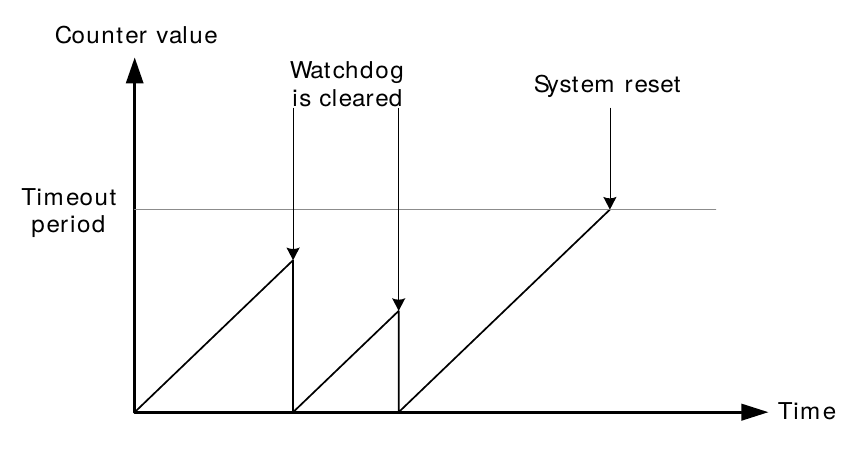
\includegraphics[width=0.85\textwidth, keepaspectratio]{imatges/Watchdog.png}
 \caption{Funcionament del {em Watchdog} \cite{EFM_AN0015}}
 \label{fig:Watchdog}
\end{figure}

La majoria de fabricants ens donen unes poques funcions per treballar amb el {\em Watchdog} (en el cas de Silicon Labs a la biblioteca EMLIB tenim el mòdul em\_wdog). Habitualment hi ha alguna funció per configurar-lo, una per engegar-lo i una per alimentar-lo. Hi ha fabricants que no permeten deshabilitar el {\em Watchdog} un cop s'ha engegat per assegurar-se que cap error de \gls{FW} provocarà que deixi de funcionar.
\index{WDOG\_Feed()}
\begin{lstlisting}[style=customc]
WDOG_Feed();
\end{lstlisting}

Habitualment es pot triar quina és la freqüència de funcionament del {\em Watchdog}, per tenir més o menys temps abans no reiniciï el sistema; normalment de pocs mil·lisegons fins a algunes desenes de segons.

\section{Exemple}
\label{sub:Watchdog_example}
En l'\href{https://github.com/mariusmm/cursembedded/tree/master/Simplicity/Watchdog}{exemple que hi ha al repositori}
es configura el {\em Watchdog} perquè treballi amb un rellotge intern de 1 kHz i que compti fins a 4097, de manera que si ningú alimenta el {\em Watchdog} en 4 segons, aquest reiniciarà el sistema. L'exemple conté un bucle que va fent blinkar el LED de la placa i una \gls{ISR} que quan es prem el botó 0 alimenta el {\em Watchdog} (Llistat~\ref{WatchdogISR}).

\index{GPIO\_EVEN\_IRQHandler()}\index{GPIO\_IntGet()}\index{GPIO\_IntClear()}\index{WDOG\_Feed()}
\begin{lstlisting}[style=customc,caption={ISR del botó que alimenta el {\em Watchdog}},label=WatchdogISR]
void GPIO_EVEN_IRQHandler(void) {
  uint32_t aux;

  aux = GPIO_IntGet();
  /* clear flags */
  GPIO_IntClear(aux);

  /* Feed watchdog */
  WDOG_Feed();
}
\end{lstlisting}

Si no premem el botó abans no passin 4 segons, el sistema es reiniciarà. I com ho veurem a l'exemple? Doncs perquè el codi el primer que fa és esbrinar per què s'està reiniciant el sistema (Llistat~\ref{Check_boot}). Si ha estat perquè ha entrat el {\em Watchdog}, el LED no blinkarà.

\begin{lstlisting}[style=customc,caption={Codi per detectar la causa del reinici},label=Check_boot]
if (resetCause & RMU_RSTCAUSE_WDOGRST) {
  resetbyWatchdog = true;
} else {
  resetbyWatchdog = false;
}
\end{lstlisting}

Cal tenir en compte que aquest dispositiu serveix per solucionar possibles fallades totals del sistema, així que cal ser curosos amb el seu ús. Així, si tenim un bucle {\bf for} que pot generar algun problema, no te sentit posar la comanda de {\em touch} al {\bf watchdog} dins del {\bf for}, si no que segurament te sentit fer-ho abans i després del bucle.

\part{Programació de perifèrics II}
\label{part:programacio_2}

\chapter{ADC}
\label{sub:ADC}
%% AMPLIAR
Un perifèric força habitual en els microcontroladors actuals és l'\gls{ADC}.

Aquesta perifèric el que fa és llegir un senyal analògic (un voltatge) i convertir-lo a un valor digital (un número). Hi ha diversos models d'\gls{ADC} amb característiques diferents, però bàsicament les característiques principals d'un ADC són:
\begin{itemize}
 \item Resolució: fa referència a quants bits dona la conversió de l'ADC. Un ADC de 16 bits, en principi, dona més detall del senyal d'entrada que un ADC de 8 bits. Actualment el més habitual és trobar ADCs d'entre 8 i 16 bits de resolució.
 \item {\em Sampling rate}: és la cadència amb la que l'ADC agafa una nova mostra del senyal i la converteix a digital. Els microcontroladors actuals incorporen ADCs que poden arribar al milió de mostres per segon.
 \item Referència: pot ser que es compari el senyal segons una referència determinada i el ADC ens doni el valor respecte a aquesta referència.
\end{itemize}

En els microcontroladors moderns, és habitual que davant de l'ADC hi hagi un multiplexor analògic, de manera que es pugui convertir diverses senyals connectades a diferents pins amb un mateix perifèric.

A l'hora de fer servir un \gls{ADC}, caldrà configurar-lo en els paràmetres de funcionament que necessitem per la nostra senyal.

Com la majoria de perifèrics, l'ADC pot generar una o vàries \glspl{IRQ} segons certes condicions, habitualment quan s'ha acabat la conversió. D'aquesta manera la CPU no cal que faci {\em polling} del registre d'estat per saber si la conversió ha finalitzat.

L'ADC acaba per donar-nos un valor dins el seu rang de treball proporcional al valor de voltatge d'entrada, aquest valor s'acostuma a anomenar {\em counts}. Per convertir aquest valor en {\em counts} al valor de voltatge corresponent, cal aplicar la fórmula \fullref{eq:ADCFormula}:
\begin{equation}
\label{eq:ADCFormula}
 V_{ADC} = \frac{{counts} * V_{max} }{2^N-1}
\end{equation}


On $V_{max}$ és el voltatge màxim de l'entrada i $N$ el nombre de bits (resolució) de la conversió de l'ADC.\footnote{Això és vàlid per configuracions tipus {\em single-ended}}

\section{Exemple d'ADC}
\label{sub:ADC_example}
\href{https://github.com/mariusmm/cursembedded/tree/master/Simplicity/ADC_1s}{Per aquest exemple} ens cal per primer cop un petit HW addicional. Farem servir un potenciòmetre que ens donarà una tensió entre Vdd i 0 volts segons el seu recorregut. La sortida d'aquest potenciòmetre la connectarem al pin 16 del connector de Debug de la PCB. Els altres dos pins aniran a 19 i 20 del mateix connector (veure esquemàtic a la Figura~\ref{fig:sch_adc} i fotografia del sistema a Figura~\ref{fig:setup_adc}).

\begin{figure}
 \centering
 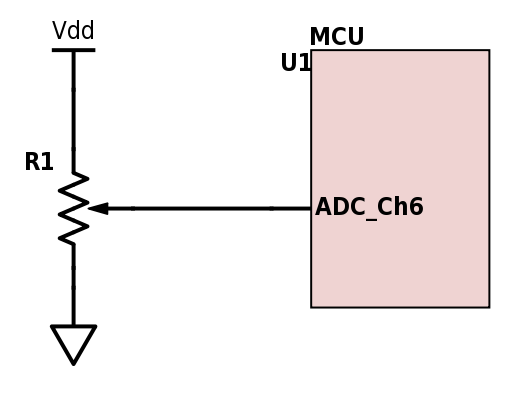
\includegraphics[width=0.85\textwidth, keepaspectratio]{imatges/adc_schematic.png}
 \caption{Esquemàtic de la connexió del Potenciòmetre al canal d'\gls{ADC}}
 \label{fig:sch_adc}
\end{figure}

\begin{figure}
 \centering
 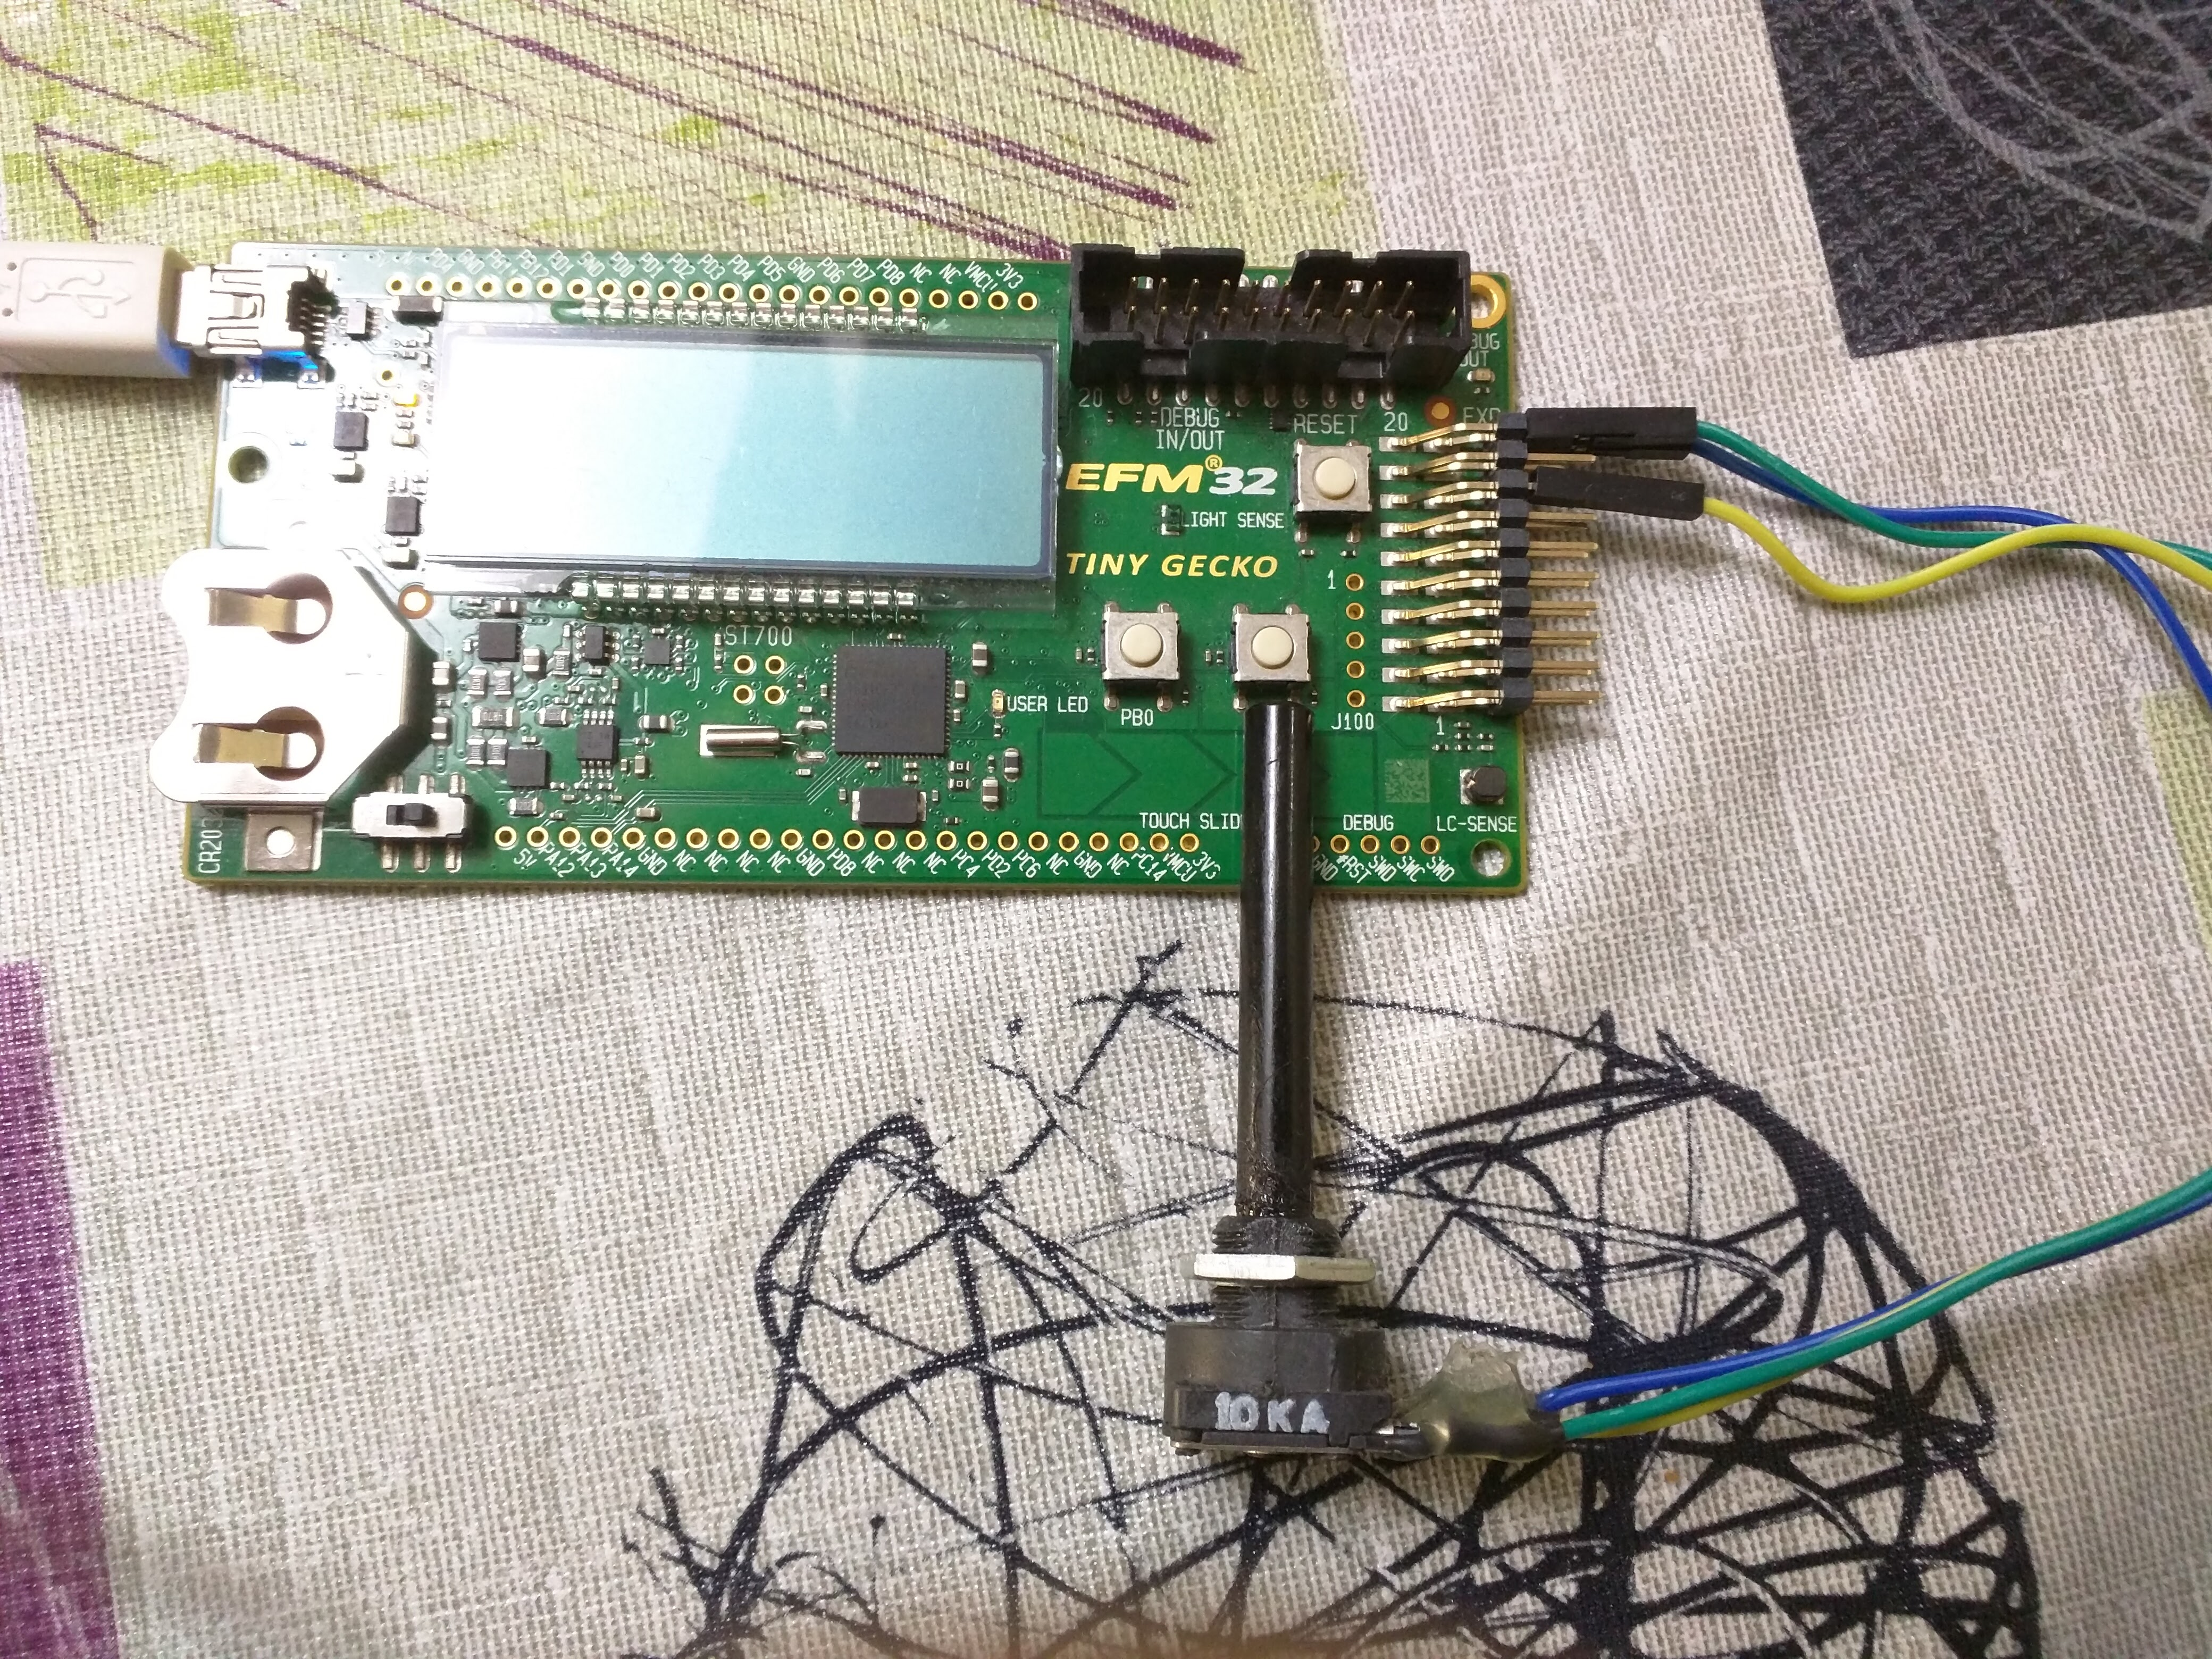
\includegraphics[width=0.85\textwidth, keepaspectratio]{imatges/adc_setup.png}
 \caption{Fotografia del sistema amb el connexitat correcte}
 \label{fig:setup_adc}
\end{figure}

Connectat així el potenciòmetre, quan estigui a un extrem del recorregut tindrem 0V a l'entrada de l'ADC i quan estigui a l'altre extrem hi tindrem \gls{Vdd}.

A l'exemple trobem un codi molt senzill, on simplement s'inicia l'\gls{ADC} amb els paràmetres per defecte i només es canvia el canal d'entrada (el 6) i la tensió de referència (en aquest cas Vdd).

D'aquesta manera, els 12 bits de resolució del ADC serviran per comparar la tensió d'entrada amb els 3.3 V amb els que està alimentat el microcontrolador a la placa.

\begin{remark}
 Els 3.3 Volts és el voltatge de funcionament de la placa d'avaluació. Els ADC normalment poden mesurar tensions fins a la seva tensió d'alimentació i és per això que en aquest cas podem mesurar fins a 3.3 Volts. Si l'alimentació fos menor, el rang de treball de l'ADC també ho seria. En el cas particular de l'ADC dels EFM32, poden tenir voltatges fixes com a referència \cite[378]{EFM32GRM}.
\end{remark}

El codi, un cop inicialitzat el ADC, realitza les accions que es veuen al Llistat~\ref{ADCSimple}.
\index{ADC\_Start()}\index{ADC\_DataSingleGet()}
\begin{lstlisting}[frame=single,caption={Codi de lectura de l'ADC},style=customc, label=ADCSimple]
while (1) {
  ADC_Start(ADC0, adcStartSingle);
  while (ADC0->STATUS & ADC_STATUS_SINGLEACT);
  ADCvalue = ADC_DataSingleGet(ADC0);
  printf("ADC Value %lu\r\n", ADCvalue);
}
\end{lstlisting}

El que fan aquests 4 línies és:
\begin{itemize}
 \item Engegar l'ADC i que comenci una conversió
 \item Esperar a que la conversió finalitzi consultant el registre STATUS de l'ADC.
 \item Llegir el valor de la conversió feta per l'ADC.
 \item Imprimir per la consola de {\em Debug} el valor de la conversió.
\end{itemize}

Per tant, el que veurem un cop engeguem l'exemple serà com es van imprimint els valors llegits per l'\gls{ADC}. Si anem movent el potenciòmetre veurem que els valors van canviant des de 0 fins a 4095.

\chapter{DAC}
\label{sub:DAC}
Un \gls{DAC} és un dispositiu que es pot veure com l'invers d'un ADC, ja que a partir d'unes dades digitals genera un senyal analògic equivalent. Els paràmetres de funcionament d'un DAC són, doncs, molt similars als del seu perifèric germà l'\gls{ADC}.

Al {\em datasheet} de la família amb la que treballem \cite[421]{EFM32GRM} hi ha la descripció, bastant breu, de les característiques principals d'aquest perifèric. Bàsicament, té un registre anomenat {\bf CHxDATA} on s'ha d'escriure el valor que volem que es converteixi a voltatge segons la fórmula següent\footnote{Pel cas single-ended, pel cas diferencial veure \cite[424]{EFM32GRM}}:
\begin{equation}
\label{eq:DACFormula}
 V_{OUT} = V_{Ref} \times \frac{CHxDATA}{4096}
\end{equation}

On $V_{Ref}$ és el voltatge de referència, que en aquest cas pot ser 2.5 o 1.25 Volts o la tensió d'alimentació Vdd.

\section{Exemple senzill amb el DAC}
\label{sec:DAC_Example_1}

Al \href{https://github.com/mariusmm/cursembedded/tree/master/Simplicity/DAC_1}{repositori} hi ha un exemple senzill usant el DAC per generar una tensió continua segons un valor donat.
Primer s'inicialitzarà el \gls{DAC} i la resta de perifèrics (en aquest cas els GPIO i poc més). Es configuren els botons com sempre, amb les dues interrupcions ja conegudes ({\bf GPIO\_ODD\_IRQHandler()}\index{GPIO\_ODD\_IRQHandler()} i {\bf GPIO\_EVEN\_IRQHandler()}\index{GPIO\_EVEN\_IRQHandler()}).

La part important de l'exemple és la inicialització del DAC, tal com es veu al Llistat~\ref{DACConfig}.

\index{CMU\_ClockEnable()}\index{DAC\_PrescaleCalc()}\index{DAC\_Init()}\index{DAC\_InitChannel()}
\begin{lstlisting}[style=customc, caption=Inicialització del DAC, label=DACConfig]
static void DACConfig(void) {
  /* Use default settings */
  DAC_Init_TypeDef init = DAC_INIT_DEFAULT;
  DAC_InitChannel_TypeDef initChannel = DAC_INITCHANNEL_DEFAULT;

  /* Enable the DAC clock */
  CMU_ClockEnable(cmuClock_DAC0, true);

  /* Set prescale for 500 KHz */
  init.prescale = DAC_PrescaleCalc(500000, 0);

  /* Set reference voltage to Vdd */
  init.reference = dacRefVDD;

  /* Initialize the DAC and DAC channel #1 */
  DAC_Init(DAC0, &init);
  DAC_InitChannel(DAC0, &initChannel, 1);
}
\end{lstlisting}

En aquest codi, primer es posen els valors per defecte que ens ofereix el fabricant i tant sols es modifiquen alguns paràmetres. Primer s'activa el {\em clock} del sistema cap al perifèric, tot seguit es tria el {\em prescaler} segons la freqüència de funcionament desitjada.  Després es selecciona que la referència per crear el senyal de sortida es basi en el voltatge d'entrada ({\bf dacRefVDD}). Per últim es configura el DAC i el canal (en aquest el 1 per la sortida que hem triat).

Les \gls{ISR} dels dos botons el que fan es incrementar o decrementar una variable global que serà el valor que s'enviarà al DAC per a que generi el senyal. Aquest increment o decrement es fa en passos de {\bf DAC\_STEP} unitats. D'aquesta manera pitjant els botons podrem seleccionar quin voltatge es genera a la sortida del DAC.

Dins el bucle infinit de la funció {\bf main()} (Llistat~\ref{DACMain}) s'envia el valor de la variable global cap al DAC amb la funció {\bf DAC\_ChannelOutputSet()}\index{DAC\_ChannelOutputSet()}, es treu el valor per la consola de debug i s'espera a que un \gls{flag} indiqui que hi ha hagut un canvi en el valor de la variable global.

\index{DAC\_ChannelOutputSet()}\index{printf()}\index{main()}
\begin{lstlisting}[style=customc, caption=Bucle infinit del DAC, label=DACMain]
void main(void) {
  while (1) {
    DAC_ChannelOutputSet(DAC0, 1, DACvalue);
    printf("DAC Value %lu (0x%06X)\r\n", (uint32_t) DACvalue, (uint32_t) DACvalue);
    while(signal == false);
    signal = false;
  }
}
\end{lstlisting}

Si mesurem el voltatge de sortida amb un multímetre, oscil·loscopi o analitzador lògic (que tingui entrada analògica) podem veure com els valors de la variable provoquen el canvi en voltatge esperat segons la Fórmula~\ref{eq:DACFormula} tal com es veu a la Taula~\ref{tb:DACVoltages}. El pin de sortida del DAC està connectat al pin PB12, connectat al pin 13 del connector d'expansió. La Taula~\ref{tb:DACVoltages} es registren tots els valors possible de la variable {\bf DACvalue}, el valor teòric que hauria de generar el DAC (segona columna) i el voltatge mesurat amb un multímetre digital (tercera columna); la quarta columna presenta la diferència entre el voltatge de la fila i l'anterior, com es pot veure cada pas corresponent a poc més de 200 mV, tal com surt a la fórmula~\ref{eq:DACFormula}. A l'última fila es calcula la mitjana aritmètica de totes aquestes diferències.


\begin{table}
\caption{Taula resum dels valors mesurats del DAC}
\centering
\begin{tabular}{|c|c|c|c|}
\hline
{\bf Variable} & {\bf Voltatge teòric (mV)} & {\bf Voltatge mesurat (mV)} & {\bf Pas}\\
\hline
0 & 0 & 0 & - \\
256	& 206 & 204 & 204 \\
512	& 413 & 410 & 206 \\
768	& 619 & 614 & 204 \\
1024	& 825 & 824 & 210 \\
1280	& 1031 & 1032 & 208 \\
1536	& 1237 & 1238 & 206 \\
1792	& 1444 & 1442 & 204 \\
2048	& 1650 & 1651 & 209 \\
2304	& 1856 &1855 & 204 \\
2560	& 2063 & 2060 & 205 \\
2816	& 2269 & 2260 & 200 \\
3072	& 2475 & 2470 & 210 \\
3328	& 2681 & 2670 & 200 \\
3584	& 2888 & 2880 & 210 \\
3840	& 3094 & 3090 & 210 \\
4096	& 3300 & 3290 & 200 \\
\hline
\multicolumn{3}{|c|}{\bf Mitjana de Pas} & 205,5 \\
%  Mitja & 205.5\\
\hline
\end{tabular}
\label{tb:DACVoltages}
\end{table}

L'exemple presentat és força bàsic i serveix per introduir la llibreria {\bf emlib} i el perifèric. A continuació veurem un exemple més complicat.

\section{Exemple més complicat amb el DAC}
\label{sec:DAC_Example_2}
En \href{https://github.com/mariusmm/cursembedded/tree/master/Simplicity/DAC_2}{aquest exemple} es farà servir el \gls{DAC} per generar un senyal periòdic tipus triangular (en anglès {\em Triangle wave}).

Es fa servir un {\em timer} per tenir una base de temps. El {\em timer} es configura a 1 kHz, dividint el rellotge d'entrada (14 MHz) entre 16 amb el {\em pre-escaler} i configurant el valor d'{\em overflow} a 875 perquè generi un senyal cada 1 mil·lisegon. Així, tindrem un nou valor cada 1 mil·lisegon i el senyal es repeteix cada 33 mostres, per tant tindrem un senyal periòdic de 30,30 Hz aproximadament (veure Equació ~\ref{eq:F_DAC_2}).

\begin{equation}
\label{eq:F_DAC_2}
 F_{senyal} = \frac{1000}{33} = 30,30 Hz
\end{equation}

El DAC es configura de la mateixa manera que a l'exemple anterior, en mode continu, amb referència al voltatge d'alimentació \gls{Vdd}. El {\em timer} es configura de manera molt similar a l'exemple vist a \fullref{sub:Timers_exemple_2}, activant les interrupcions per tenir la ISR executant-se cada 1 mil·lisegon.

A la \gls{ISR} del {\em timer} es calcula el nou valor pel \gls{DAC} i s'escriu el nou valor calculat (veure Llistat~\ref{DAC_2_Example}).

\index{TIMER0\_IRQHandler()}\index{DAC\_ChannelOutputSet()}
\begin{lstlisting}[style=customc, caption=Part de la ISR del Timer per generar la dada pel DAC, label=DAC_2_Example]
void TIMER0_IRQHandler(void) {
  ...
  if (direction_up == true) {
    DACvalue += DAC_STEP;
    if (DACvalue >= 0x1000) {
      DACvalue = 0x0FFF;
      direction_up = false;
    }
  } else {
    DACvalue -= DAC_STEP;
    if (DACvalue < 0) {
      DACvalue = 0;
      direction_up = true;
    }
  }
  DAC_ChannelOutputSet(DAC0, 1, DACvalue);
}
\end{lstlisting}

A l'hora d'executar el codi, si es connecta un oscil·loscopi o analitzador lògic al pin 13 del connector d'expansió de la placa de desenvolupament, que es correspon al pin PB12 del microcontrolador es veurà el senyal com es mostra a la Figura~\ref{fig:DAC_result}. Es pot observar com cada esglaó dura 1 mil·lisegon i els increments són de 200 mV aproximadament (Figura~\ref{fig:DAC_result_zoom}).

\begin{figure}
 \centering
 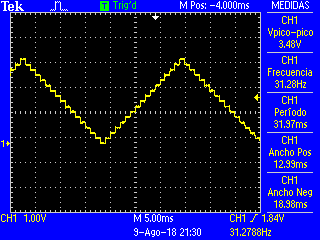
\includegraphics[width=0.65\textwidth, keepaspectratio]{imatges/DAC_result_osc}
 \caption{Senyal capturat per l'oscil·loscopi.}
 \label{fig:DAC_result}
\end{figure}

\begin{figure}
 \centering
 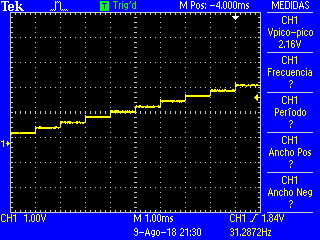
\includegraphics[width=0.65\textwidth, keepaspectratio]{imatges/DAC_result_osc_zoom}
 \caption{Detall del senyal capturat per l'oscil·loscopi}{Detall del senyal capturat per l'oscil·loscopi, es pot veure que la unitat de temps és d'1 mil·lisegon.}
 \label{fig:DAC_result_zoom}
\end{figure}

En aquest exemple s'ha presentat com generar un senyal periòdic mitjançant el \gls{DAC} i un {\em Timer}, aquesta combinació de perifèrics és força habitual per generar senyals d'aquesta mena donada la seva senzillesa i facilitat d'ús.

En cas que els valors del senyal estiguessin pre-calculats i emmagatzemats en una taula, la \gls{ISR} del {\em Timer} només caldria agafar el següent valor de la taula.

\chapter{UART}
\label{sub:UART}
El port sèrie és encara un dels ports d'entrada i sortida més comuns de trobar en un microcontrolador i en un sistema encastat. Encara avui multitud de dispositius fan servir aquest port per rebre o enviar dades i, per tant, els microcontroladors acostumen a incloure uns quants d'aquests ports.

Aquest port sèrie en els microcontroladors el gestiona un perifèric anomenat \gls{USART} (o \gls{UART}). El port sèrie habitual, basat en l'estàndard RS-232 només té dos fils, un per rebre dades (RX) i un per enviar-ne (TX). La velocitat i les característiques de la transmissió es poden configurar i habitualment s'envien 8 bits per caràcter amb 1 bit d'stop i sense paritat (tot i que es pot canviar). Les velocitats de transmissió més habituals són: 9600 \gls{bps}, 19200 bps, 56700 bps i 115200 bps. El que cal, com és obvi, és configurar el port sèrie del microcontrolador amb els mateixos paràmetres que el dispositiu extern que estiguem usant.

L'altre aplicació pràctica del port sèrie és poder connectar el microcontrolador a un ordinador personal per poder interactuar amb ell, ja sigui per enviar dades, informació d'estatus o rebre comandes o paràmetres de configuració. Com que actualment la majoria d'ordinadors no tenen un port sèrie, s'han popularitzat molt uns petits dispositius que converteixen el port sèrie en un \gls{USB} de tipus sèrie. D'aquest dispositiu conegut com \gls{CP2102} en parlarem més endavant.

\section{Fent servir una USART}
Com que la configuració d'un port sèrie és una mica complicada, sobretot perquè segons la velocitat de funcionament del rellotge del sistema caldrà dividir i multiplicar aquest senyal fins a tenir una velocitat adequada per la velocitat seleccionada pel port sèrie, els fabricants acostumen a donar-nos biblioteques que ens ajuden.

Dins la biblioteca acostumen a oferir una funció per enviar dades ({\bf USART\_Tx()}\index{USART\_Tx()}) i una per rebre'n ({\bf USART\_RX()}\index{USART\_Rx()}). Aquestes funcions són molt senzilles, i permeten enviar un sol byte o rebre'n un, o espera-se indefinidament fins que n'arribi un. Això pot ser que no sigui l'ideal per la nostra aplicació i les \gls{USART} permeten generar interrupcions segons certs esdeveniments. Normalment els més usats són el de byte rebut i el de byte enviat. D'aquesta manera, ens podem muntar una biblioteca que ens permeti rebre dades pel port sèrie fent servir exclusivament interrupcions i a la nostra aplicació agafem el que s'hagi rebut quan vagi bé.

La manera més habitual d'implementar aquest mecanisme asíncron de enviar o rebre dades pel port sèrie és mitjançant un \gls{buffer circular}. D'aquesta manera, la \gls{ISR} de recepció ({\bf USART1\_RX\_IRQ\\Handler()}\index{USART1\_TX\_IRQHandler()}) insereix la nova dada rebuda al {\em buffer} de recepció cada cop que la criden. Només cal escriure una funció a la nostra biblioteca que extregui un caràcter del {\em buffer} cada cop que la cridin i escriure una funció que retorni el nombre de caràcters disponibles al {\em buffer} (veure Llistat \ref{UARTISRs}).

La ISR de transmissió ({\bf USART1\_TX\_IRQHandler()}\index{USART1\_TX\_IRQHandler()}) es crida cada cop que s'acaba d'enviar un caràcter, per tant la ISR pot enviar un caràcter del {\em buffer} circular de transmissió cada cop que la cridin (quan s'ha acabat d'enviar el caràcter anterior) i ens cal una funció que copiï les dades a enviar cap al {\em buffer} circular de transmissió i engegui el procés.

\index{USART\_IntClear()}\index{USART\_Send()}\index{USART\_Rx()}
\begin{lstlisting}[style=customc,caption={ISRs de TX i RX de la UART},label=UARTISRs]
void USART1_TX_IRQHandler(void) {
  USART_IntClear( USART1, USART_IEN_TXC);
  USART_Send(USART1);
}

void USART1_RX_IRQHandler(void) {
  char data;

  if (USART1->IF & LEUART_IF_RXDATAV) {
    data = USART_Rx(USART1);
    PushData(data, &RX_SerialBuffer);
    USART_IntClear( USART1, USART_IEN_RXDATAV);
  }
}
\end{lstlisting}



\section{Exemple d'ús d'una UART}
\label{sub:UART_example}
Per fer les proves caldrà tenir a mà un dispositiu \gls{CP2102}. Aquest dispositiu conté un xip, el CP2102 que per un costat té un port sèrie i per l'altre un port USB de tipus {\em Virtual COM Port Device} que qualsevol ordinador, ja sigui Windows, GNU/Linux o Mac reconeixen com un port sèrie. D'aquesta manera, fent servir aquest dispositiu podem connectar un microcontrolador amb un port sèrie a un ordinador de sobretaula o portàtil que tingui un port \gls{USB} lliure.

Ara el que cal és preparar-ho tot: preparar el codi, connectar el mòdul CP2102 a la nostra placa de prototipat i connectar-la per USB a un ordinador.

El \href{https://github.com/mariusmm/cursembedded/tree/master/Simplicity/UART_1}{codi que hi ha al repositori} primer configura la USART1 del microcontrolador perquè funcioni a 115200 bps, 8 bits per caràcter, sense paritat i 1 bit d'stop, que ve a ser la configuració estàndard d'un port sèrie. També en el mateix bloc configura els dos pins del port (TX i RX). També configura com s'ha d'enrutar la USART1, en aquest cas cap la localització 1 que es correspon als pins PD0 i PD1 del microcontrolador, que estan connectats al connector d'expansió, als pins 4 i 6 respectivament (veure Figura~\ref{fig:CP2102}). Tot seguit s'envia un caràcter ‘A' pel port sèrie.

A continuació es configuren els dos botons perquè generin una \gls{IRQ}. A les \glspl{ISR} tant sols es canvia el LED (un botó l'encén i l'altre l'apaga) i un botó envia una ‘A' i l'altre botó envia un ‘B'.

Per veure aquests caràcters al nostre ordinador, primer cal connectar el mòdul CP2102 a la nostra placa pel connector d'expansió tal com es veu a la foto. Un cop connectem el CP2102 al nostre ordinador, cal engegar algun programa de terminal pel port sèrie, tipus {\em putty} \cite{putty}, {\em minicom}, {\em Tera Term} \cite{teraterm}, etc.

\begin{remark}
 També es pot instal·lar un terminal dins del {\bf Simplicity Studio}. Cal anar a l'{\em Eclipse Marketplace}, buscar el {\bf TM Terminal} i instal·lar-lo \cite{tmterminal}. Així tindrem el terminal integrat dins el IDE.
\end{remark}

\begin{figure}
 \centering
 \includegraphics[width=0.85\textwidth, keepaspectratio]{imatges/img_20180302_162857.png}
 \caption{Connexió del CP2102 a la placa de prototipat}
 \label{fig:CP2102}
\end{figure}


\section{Un exemple amb la UART més complicat}
\label{sec:UART_example_2}
Un cop vist un exemple senzill de com es configura una USART, anem a fer un exemple més complex, rebent i enviant dades del microcontrolador cap al PC i a l'inrevés. El codi està al \href{https://github.com/mariusmm/cursembedded/tree/master/Simplicity/UART_2}{repositori}.

En aquest cas farem servir \glspl{buffer circular} per guardar les dades rebudes o a enviar.  És una implementació senzilla d'un buffer circular sense gaire secrets, l'hem posat a la biblioteca {\bf CircularBuffer}. Aquesta biblioteca ofereix unes funcions molt senzilles per gestionar el buffer circular:
\begin{itemize}
 \item {\bf PushData()}\index{PushData()} que permet inserir un caràcter al {\em buffer}
 \item {\bf PopData()}\index{PopData()} que retorna el següent caràcter del {\em buffer}
 \item {\bf AvailableData()}\index{AvailableData()} que indica la quantitat de caràcters disponibles al {\em buffer}
\end{itemize}

En aquest exemple es fan servir les interrupcions de la USART per controlar-la, de manera que al rebre un caràcter, la \gls{ISR} corresponent l'insereix al {\em buffer} corresponent (hi ha dos {\em buffer}, un de recepció i un d'enviament), veure Llistat~\ref{ISR_UARTRX_Avançada} i \ref{ISR_UARTTX_Avançada}.
\index{USART1\_RX\_IRQHandler()}\index{USART\_Rx()}\index{USART\_IntClear()}
\begin{lstlisting}[style=customc,label=ISR_UARTRX_Avançada,caption=Exemple ISR avançada]
void USART1_RX_IRQHandler(void) {
  char data;

  if (USART1->IF & LEUART_IF_RXDATAV) {
    data = USART_Rx(USART1);
    PushData(data, &RX_SerialBuffer);
    USART_IntClear( USART1, USART_IEN_RXDATAV);
  }
}
\end{lstlisting}

D'aquesta manera, en qualsevol moment que es rebi un caràcter per la UART, la \gls{ISR} el guardarà el {\em buffer} {\bf RX\_SerialBuffer} i seguirà l'execució el nostre programa.

Quan calgui, podrem cridar a la funció {\bf AvailableData()}\index{AvailableData()} per saber si hem rebut alguna cosa i processar-la si cal.

Per enviar dades, cal que primer omplim el \gls{buffer circular} corresponent ({\bf TX\_SerialBuffer}) amb el que vulguem enviar i després cridar la funció {\bf USART\_Send()}\index{USART\_Send()}. D'aquesta manera, i gràcies a que hem configurat la USART perquè llenci una \gls{IRQ} cada cop que acabi d'enviar un caràcter, la USART enviarà un primer caràcter i es cridarà la ISR, que tornarà a cridar la funció d'enviar un caràcter fins que no en quedi cap més al {\em buffer}.

\index{USART1\_TX\_IRQHandler()}\index{USART\_IntClear()}\index{USART\_Send()}
\begin{lstlisting}[style=customc,label=ISR_UARTTX_Avançada,caption=Exemple ISR avançada]
void USART1_TX_IRQHandler(void) {
  USART_IntClear( USART1, USART_IEN_TXC);
  USART_Send(USART1);
}
\end{lstlisting}

Fent servir les interrupcions alliberem el processador d'esperar a que la USART vagi enviant els caràcters un a un i ens podem dedicar a fer altres coses (Llistat~\ref{UART_example_2}).

\begin{lstlisting}[style=customc,label=UART_example_2,caption=Funció main]
while (1) {
  if (AvailableData(&RX_SerialBuffer) != 0) {
    character = PopData(&RX_SerialBuffer);
    /* Prepare the buffer with the data to be sent */
    PushData(character, &TX_SerialBuffer);
    PushData(character + 1, &TX_SerialBuffer);
    PushData(character + 2, &TX_SerialBuffer);
    /* Start send process */
    USART_Send(USART1);
  }
}
\end{lstlisting}


\chapter{I2C}
\label{sub:I2C}
Quan parlem de busos per comunicar dispositius i sensors amb un microcontrolador, el bus \gls{I2C} és un dels primers que venen al cap (l'altre és el bus \gls{SPI}, veure \fullref{sub:SPI}).

Presentat per Philips fa una pila d'anys, ha acabat sent un dels dos busos {\em estàndard de facto} per comunicació interPCBs (l'altre, com ja hem dit, és l'\gls{SPI}). És un bus multi-master i multi-slave, que vol dir que poden haver més d'un dispositiu esclau i varis dispositius mestres funcionat al bus (tot i que només es pot comunicar un màster amb un slave alhora). El bus I2C funciona amb només dues línies: una transporta el rellotge del bus (\gls{SCL}) i l'altra les dades entre tots els dispositius (\gls{SDA}). Totes dues línies són de tipus {\em open-drain} i per tant necessita de resistències de {\em pull-up} pel seu correcte funcionament. La freqüència de funcionament pot ser com a màxim de 100 kHz (o de 400 kHz en mode fast) tot i que pot normalment pot funcionar a qualsevol freqüència inferior.

Cada un dels dispositius té una adreça de 7 bits que ha de ser única al bus i que serveix per adreçar-s'hi per part d'altres dispositius. Una transferència típica consisteix en un Master que posa al bus l'adreça del dispositiu Slave que vol accedir amb el bit menys significatiu a 0 o 1 segons vulgui accedir-hi per llegir ('1') o per escriure ('0'), a continuació posa l'adreça del registre (o adreça de memòria) que vol llegir o escriure i a continuació la dada a escriure o la dada de resposta. La unitat de treball del bus és de 8 bits (1 byte) així que si cal transmetre més dades caldrà enviar les dades byte a byte\footnote{Hi ha un mode d'I2C que amplia la longitud de l'adreça de 7 a 10 bits}.

Tenim multitud de dispositius de tota mena que tenen aquest bus com sistema de comunicació amb el microcontrolador i és força comú en sensors digitals, memòries EEPROM, expansió d'I/O, \glspl{ADC}, \glspl{DAC}, etc. i la majoria de microcontroladors inclouen un perifèric tipus Màster.

\begin{figure}
 \centering
 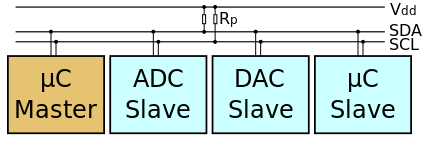
\includegraphics[width=0.85\textwidth, keepaspectratio]{imatges/I2C.png}
 \caption{Esquema d'un bus I2C típic}{Esquema d'un bus I2C típic. Font: user:Cburnett (Own work made with Inkscape) [GFDL o CC-BY-SA-3.0], via la Wikimedia Commons}
 \label{fig:I2C}
\end{figure}

\section{Exemple d'I2C}
\label{sub:I2C_example}
Per aquest exemple farem servir el sensor de gestos, de llum i de proximitat {\bf APDS-9960} de Broadcom \cite{apds9960}. Es pot adquirir una placa de prototipat a la web Sparkfun per poder provar-lo ràpidament. La placa té un connector força estàndard amb els pins d'alimentació, massa, les dues línies del \gls{I2C} \gls{SCL} i \gls{SDA}, i un pin d'interrupció.

Per connectar aquesta \gls{PCB} a la nostra placa de prototipat, farem servir 4 cables i els connectarem seguint la Taula~\ref{tb:I2C}.

\begin{table}
\caption{Connexionat de la placa APDS-9960 i la placa de prototipat}
\label{tb:I2C}
\centering
\begin{tabular}{|c|c|}
\hline
{\bf SiliconLabs (Expansion header)}	 & {\bf APDS-9960 PCB Board}\\
\hline
15 & SCL\\
\hline
16 & SDA\\
\hline
19 & GND\\
\hline
20 & VDD\\
\hline
\end{tabular}

\end{table}

Amb això estem connectant directament els pins del microcontrolador que poden fer de màster \gls{I2C} als pins sensor que fa d'slave I2C. Les resistències de \gls{pull-up} que calen per tot bus I2C estan a la PCB d'sparkfun (veure a l'esquemàtic aquí les resistències R2 i R3).

Un cop tenim el Hardware preparat, cal posar-se amb el Firmware. Per fer servir el controlador Màster del nostre microcontrolador podem fer sevir les llibreries de SiliconLabs emlib. \href{https://github.com/mariusmm/cursembedded/tree/master/Simplicity/I2C_1}{Aquí està el projecte sencer} per EFM32.

El primer que cal fer és activar el rellotge per aquest perifèric i configurar els pins corresponents. En aquest cas, els pins 15 o 16 del connector corresponent als pins PD7 i PD6 respectivament, que són la {\em localization \#1} del I2C d'aquest microcontrolador (Llistat~\ref{i2cpins}).
\index{CMU\_ClockEnable()}\index{GPIO\_PinModeSet()}
\begin{lstlisting}[frame=single,style=customc, label=i2cpins, caption={Initialització dels pins per l'I2C}]
CMU_ClockEnable(cmuClock_I2C0, true);
GPIO_PinModeSet(gpioPortD, 7, gpioModeWiredAnd, 1);
GPIO_PinModeSet(gpioPortD, 6, gpioModeWiredAnd, 1);

I2C0->ROUTE = I2C_ROUTE_SDAPEN | I2C_ROUTE_SCLPEN |
        I2C_ROUTE_LOCATION_LOC1;
\end{lstlisting}

A continuació cal configurar el perifèric màster, podem deixar-ho tot amb les opcions per defecte (Llistat~\ref{i2cconfig}).

\index{I2C\_Init()}
\begin{lstlisting}[frame=single,style=customc,label=i2cconfig, caption={Inicialització del perifèric I2C}]
I2C_Init_TypeDef i2cInit = I2C_INIT_DEFAULT;
I2C_Init(I2C0, &i2cInit);
\end{lstlisting}

Un cop fet això, ja podem fer servir el controlador I2C per accedir als dispositius que hi hagin al bus.

Per comoditat, s'acostuma a munta una funció per llegir registres i una funció per escriure'n. Veiem la funció {\bf I2C\_ReadRegister()}\index{I2C\_ReadRegister()} (Llistat~\ref{I2CReadRegister}).
\index{I2C\_TransferInit()}\index{I2C\_Transfer()}
\begin{lstlisting}[style=customc,caption=Funció {\bf I2C\_ReadRegister},label=I2CReadRegister]
static bool I2C_ReadRegister(uint8_t reg, uint8_t *val) {
  I2C_TransferReturn_TypeDef I2C_Status;
  I2C_TransferSeq_TypeDef seq;
  uint8_t data[2];

  seq.addr = DEVICE_ADDR;
  seq.flags = I2C_FLAG_WRITE_READ;
  seq.buf[0].data = &reg;
  seq.buf[0].len = 1;
  seq.buf[1].data = data;
  seq.buf[1].len = 1;

  I2C_Status = I2C_TransferInit(I2C0, &seq);

  while (I2C_Status == i2cTransferInProgress) {
    I2C_Status = I2C_Transfer(I2C0);
  }
  if (I2C_Status != i2cTransferDone) {
    return false;
  }
  *val = data[0];
  return true;
}
\end{lstlisting}

El primer que fem és definir les variables que ens caldran. La variable més estranya que veiem aquí és la variable {\bf seq} de tipus {\bf I2C\_TransferSeq\_TypeDef}. En aquesta estructura és on es guarda tota la informació necessària per engegar una transacció per part del controlador dins el microcontrolador. Per tant, a l'estructura cal posar-hi l'adreça \gls{I2C} del dispositiu, quina mena de transacció es vol fer (lectura, escriptura, etc.), en aquest cas {\bf I2C\_FLAG\_WRITE\_READ}, que vol dir que volem llegir d'un registre; també cal omplir una {\em array} d'estructures ({\bf buf[]}) on es guarda les dades a enviar o a rebre. En aquest cas, com que només volem llegir un registre (un sol byte) al {\bf buf[0]} només hi posem l'adreça del registre a llegir i la longitud a 1 i a {\bf buf[1]} li posem un {\em buffer} per emmagatzemar el valor llegit i de longitud 1 sol byte per llegir.

Un cop omplerta aquesta estructura s'engega la transacció amb la crida {\bf I2C\_TransferInit()}\index{I2C\_TransferInit()}, que retorna un {\bf I2C\_Status}. Després, tal com ens demana la biblioteca EMLIB, cal anar cridant la funció {\bf I2C\_Transfer()}\index{I2C\_Transfer()} mentre la variable {\bf I2C\_Status} valgui {\bf i2cTransferInProgress}. Això indica que la transferència pel bus s'ha acabat i cal veure com ha anat l'operació. Si tot ha anat bé la variable {\bf I2C\_Status} valdrà {\bf i2cTransferDone}. Així, el que tenim és una funció que li passem l'adreça del registre que volem llegir i ens retorna el valor que ens retorna el dispositiu.

Ara tornem al nostre sensor de gestos. Quasi tots els dispositius I2C tenen un registre de tipus identificació, que ens permet validar que la comunicació es fa realment amb ell. En el cas del APDS-9960 té un registre anomenat ‘ID' a l'adreça 0x92 i que el valor que retorna al llegir-lo és 0xAB (pàgina 25 del {\em Datasheet} \cite{apds9960}). Ara toca, doncs, muntar una funció que comprovi que s'està correctament a aquest dispositiu com es veu al Llistat~\ref{testI2C}.

\index{testI2C()}\index{I2C\_ReadRegister()}
\begin{lstlisting}[style=customc,caption=Funció {\bf testI2C()},label=testI2C]
void testI2C(void) {
  uint8_t ret_value;

  I2C_ReadRegister(0x92, &ret_value);

  if (ret_value == 0xAB) {
    printf("Detected!\r\n");
  } else {
    printf("Something went wrong\r\n");
  }
}
\end{lstlisting}

Ara només cal ajuntar-ho tot en el nostre main i ja podem comprovar que tenim la PCB ben connectada i funcionant. Farem servir aquest bus i el mateix dispositiu a l'exemple tractat a \fullref{ch:aplicaciosenzilla}.


\chapter{SPI}
\label{sub:SPI}
El bus \gls{SPI} és un altre dels busos més populars usats en sistemes encastats. Aquest sistema de comunicació no és un bus pròpiament dit, donat que ens permet connectar un {\em Master} amb un {\em Slave} i només de forma indirecta connectar més {\em Slaves}.
Aquest bus es basa en dues línies per enviar o rebre dades, batejades \gls{MOSI} i \gls{MISO} segons la dada vagi del {\em Master} cap a l'{\em Slave} o a l'inrevés. Com és un bus síncron, hi ha una tercera línia que porta el rellotge (\gls{SCLK}) i que el genera el {\em master}. Per últim, hi ha una quarta línia de control, normalment anomenada \gls{SS} que indica a un {\em slave} concret que la transmissió és per ell. Controlant correctament un conjunt d'aquestes línies \gls{SS} és possible tenir més dispositius {\em slaves} al connectats al bus (Figura~\ref{fig:SPI}). Aquesta línia pot no usar-se, i llavors es parla d'un SPI de 3 fils enlloc d'un SPI de 4 fils.


\begin{figure}
 \centering
 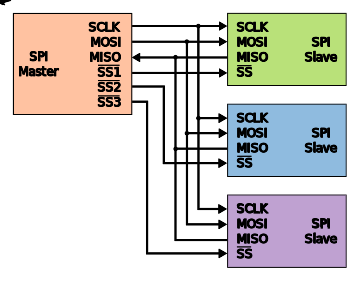
\includegraphics[width=0.85\textwidth, keepaspectratio]{imatges/SPI_three_slaves.png}
 \caption{Bus SPI típic}{Bus SPI típic. Per en:User:Cburnett [GFDL (http://www.gnu.org/copyleft/fdl.html) o CC-BY-SA-3.0 (http://creativecommons.org/licenses/by-sa/3.0/)], de la Wikimedia Commons}
 \label{fig:SPI}
\end{figure}




Aquest bus acostuma a poder treballar a força més velocitat que el bus \gls{I2C}, i és habitual configurar-lo per freqüències de rellotge d'uns pocs MHz (és habitual treballar amb freqüències d'1, 10 o fins i tot 24 MHz). En tot cas, cal consultar sempre les especificacions dels dispositius {\em slave} per saber la velocitat màxima de treball.

Precisament per aquesta característica, que fa que es puguin enviar moltes més dades per segon, els dispositius que incorporen un bus SPI acostumen a ser sensor i dispositius que generen un gran volum de dades de forma continua, com ara: \glspl{ADC}, memòries RAM i \gls{FLASH}, LCDs, targetes SD,  alguns sensors concrets, etc.

Com que aquest bus no està pensat per tenir més d'un {\em slave} connectat simultàniament, no incorpora el concepte d'adreça de dispositiu. A diferència del \gls{I2C}, que el propi bus especifica com és el protocol per accedir a un registre, en el SPI aquesta definició és pròpia de cada fabricant. Tot i això, habitualment el primer camp de la transmissió és l'adreça del registre a accedir o la comanda a executar.

En alguns microcontroladors el control d'aquest bus el fa el perifèric USART (veure \fullref{sub:UART}) configurat pertinentment, com és el cas de les famílies de microcontroladors de Silicon Labs \cite[207]{EFM32GRM}, i d'altres famílies incorporen perifèrics dedicats en exclusiva a aquest bus, com els de ST \cite[873]{STM32F4RM}.

\chapter{DMA}
\label{sub:DMA}
El \gls{DMA} és un dispositiu present a la majoria de microprocessadors. Aquest dispositiu s'encarrega de fer transferències de dades entre dispositius o memòria sense que la CPU intervingui.

Per què es fa servir? Doncs perquè sovint cal transferir quantitats importants de dades entre dues parts de la memòria, o anar transferint dades d'un dispositiu cap a un {\em buffer} a la memòria i no cal que la CPU estigui entretinguda fent això quan podria fer alguna cosa més interessant o en un mode de baix consum (veure~\fullref{ch:low-power}).

Els DMA acostumen a tenir diferents canals que poden fer transferències per separat i en paral·lel, de manera que podem tenir un canal preparat per moure regions de memòria, un altre per enviar dades cap a un DAC, un tercer transferint les dades rebudes per la UART, etc. Aquest diferents canals acostumen a estar prioritzats, de manera que l'àrbitre del bus pot decidir quin canal ha de poder accedir abans que un altre.

Normalment el dispositiu DMA es configura mitjançant descriptors, que són unes estructures on es guarda el tipus de transferència, l'adreça d'origen, l'adreça de destí, etc. Un cop s'engega la transferència, el DMA anirà movent les dades d'una adreça a l'altra segons s'hagi configurat. A la majoria de DMAs moderns, a més, es pot configurar el DMA de manera que copiï una dada d'un determinada adreça (que correspon a un registre de dades d'un perifèric) cada cop que el perifèric llença una notificació, de manera que el DMA fa una còpia d'una dada cada cop que el dispositiu en genera una. Tot això es veurà millor amb dos exemples.

\section{Exemple}
\label{sub:DMA_example}
Posar un exemple de \gls{DMA} sovint és complicat, ja que involucra força perifèrics diferents i configuracions, així que intentarem fer algun de simple per començar. Per aquest \href{https://github.com/mariusmm/cursembedded/tree/master/Simplicity/DMA_1}{primer exemple} hem optat per fer una transferència entre dues regions de memòria amb el DMA. Per això, tindrem un buffer d'origen i un de destí, en aquest cas de 256 elements de 32 bits cadascun (uint32\_t src\_buffer[BUFFER\_SIZE]).

El primer que es fa és inicialitzar el DMA amb les funcions d'emlib corresponents.
\index{DMA\_Init()}
\begin{lstlisting}[caption={Inicialització del DMA},style=customc]
dma_init.hprot = 0;
dma_init.controlBlock = dmaControlBlock;
DMA_Init(&dma_init);
\end{lstlisting}

La variable {\bf dmaControlBlock} és un {\em array} on es guarden els descriptors de cada un dels canals disponibles del DMA (Llistat~\ref{dmaControlBlock}).
\begin{lstlisting}[style=customc, caption={Definició de la variable {\bf dmaControlBlock}}, label=dmaControlBlock]
DMA_DESCRIPTOR_TypeDef dmaControlBlock[DMACTRL_CH_CNT * 2] SL_ATTRIBUTE_ALIGN(DMACTRL_ALIGNMENT);
\end{lstlisting}

A continuació configurem un canal del DMA (Llistat~\ref{DMAchannelconfig}) i li assignem una funció de \gls{callback} perquè ens notifiqui quan ha acabat la transferència (Llistat~\ref{DMAComplete}):
\index{DMA\_CfgChannel()}
\begin{lstlisting}[style=customc, caption={Configuració del canal DMA}, label=DMAchannelconfig]
dma_cb.cbFunc = DmaComplete;
dma_cb.userPtr = NULL;

dma_chn.enableInt = true;
dma_chn.highPri = false;
dma_chn.select = 0; /* set to 0 because is a memory-to-memory transfer */
dma_chn.cb = &dma_cb;
DMA_CfgChannel(0, &dma_chn);
\end{lstlisting}

\begin{lstlisting}[style=customc,caption={Callback del DMA {\bf DmaComplete()}\index{DmaComplete()}},label=DMAComplete]
void DmaComplete(unsigned int channel, bool primary, void *user) {
  dma_end = true;
}
\end{lstlisting}
També s'activen les interrupcions (necessàries per tenir \glspl{callback}) i es selecciona com serà la transferència (en aquest cas un 0 per indicar que serà de memòria a memòria).

Per últim es configura el descriptor de la transferència (Llistat~\ref{paramDMA}).
\index{DMA\_CfgDescr()}
\begin{lstlisting}[style=customc, caption={Paràmetres de configuració del DMA}, label=paramDMA]
dma_descr.arbRate = dmaArbitrate1;
dma_descr.dstInc = dmaDataInc4;
dma_descr.hprot = 0;
dma_descr.size = dmaDataSize4;
dma_descr.srcInc = dmaDataInc4;
DMA_CfgDescr(0, true, &dma_descr);
\end{lstlisting}

En aquest cas es tria com ha de manegar les adreces (tant a la font com al destí) i quants bytes es transfereixen a cada accés. Com que estem movent un {\em array} de 32 bits de paraula, triem incrementar de 4 en 4 l'adreça i moure 4 bytes a cada accés.

Per últim activem la transferència \gls{DMA} com es veu al Llistat~\ref{activateDMA}.
\index{DMA\_ActivateAuto()}
\begin{lstlisting}[style=customc, caption={Activació de la transferència DMA}, label=activateDMA]
DMA_ActivateAuto(0, true, dst_buffer, src_buffer, BUFFER_SIZE - 1);
\end{lstlisting}

Aquí la única particularitat és que cal especificar-li el nombre d'accessos a fer per completar la transferència, però restant-li un\footnote{Això és una particularitat de la biblioteca EMLIB de {\em Silicon Labs}} i altres biblioteques poden necessitar paràmetres lleugerament diferents.

A l'exemple es fa servir una variable global ({\em volatile}!) de nom {\bf dma\_end} que la \gls{callback} posa a {\em true} per notificar a la funció {\bf main()} que la transferència s'ha acabat. Quan això passa, es comprova que els dos {\em buffers} són iguals (Llistat~\ref{Check_buffers}) i es presenta per la consola.

\index{check\_buffers\_copy()}
\begin{lstlisting}[style=customc, caption={Comparació dels dos buffers de l'exemple DMA}, label=Check_buffers]
bool check_buffers_copy() {
  int i;

  for (i=0; i<BUFFER_SIZE; i++) {
    if (dst_buffer[i] != src_buffer[i]) {
      return false;
    }
  }
  return true;
}
\end{lstlisting}


\section{Un exemple amb DMA més complicat}
\label{sec:DMA_example_2}

Una altra aplicació del \gls{DMA} és transferir dades cap o des de un perifèric cap a memòria sense que el processador ho hagi de fer. Un exemple és fer servir el DMA per rebre o transferir dades cap al port sèrie. Així, enlloc d'anar llençant una \gls{IRQ} cada cop que el microcontrolador pot enviar la següent dada, es pot configurar el DMA per a que ho faci ell mateix de forma automàtica Anem a veure com es fa això modificant el \href{https://sistemesencastats.wordpress.com/2018/03/08/serie-i-usb-cp2102/}{segon exemple sobre la UART} (comentat a la \fullref{sec:UART_example_2}).

Així, el que farem en aquest exemple és deixar el \gls{buffer circular} i el mateix mecanisme per rebre dades de la {\bf USART (RX)} però canviarem la manera en que enviem les dades (TX). L'exemple és \href{https://github.com/mariusmm/cursembedded/tree/master/Simplicity/UART_DMA}{aquí}.

El que farem és preparar el DMA per a que transfereixi dades des d'un {\em buffer} a la memòria cap al registre d'enviament de la USART (registre {\bf TXDATA} de la USART1). En aquest cas, cal configurar-lo que no incrementi l'adreça de destí, que incrementi la font byte a byte i que transfereixi bytes (els caràcters d'una UART són bytes). També cal especificar quin dispositiu fa de {\em trigger}, és a dir, quin dispositiu notifica que té una dada disponible per ser transferida (paràmetre dma\_chn.select = DMAREQ\_USART1\_TXBL). En aquest exemple no ens cal saber quan el \gls{DMA} ha acabat la transferència, així que no registrem cal \gls{callback} ni activem les interrupcions del DMA. Tot això ho hem encapsulat a la funció {\bf my\_DMA\_Init()}\index{my\_DMA\_Init()} (Llistat~\ref{DMAinit_2}).

\index{my\_DMA\_Init()}
\begin{lstlisting}[style=customc,caption={Diferències a la inicialització del DMA}, label=DMAinit_2]
void my_DMA_Init(void) {
  ...
  dma_chn.select = DMAREQ_USART1_TXBL;
  ...
  dma_descr.dstInc = dmaDataIncNone;
  dma_descr.size = dmaDataSize1;
  dma_descr.srcInc = dmaDataInc1;
  ...
}
\end{lstlisting}

Ens cal també una funció que engegui la transferència del DMA cap a la UART. Li hem dit {\bf sendUARTbyDMA()}\index{sendUARTbyDMA()} i rep com a paràmetres el {\em buffer} a enviar i la seva longitud (en bytes). Aquesta funció tan sols espera que el DMA no estigui ocupat i tot seguit engega la transferència (veure Llistat~\ref{lst:sendUARTbyDMA}).

\index{sendUARTbyDMA()}\index{DMA\_ChannelEnabled()}\index{DMA\_ActivateBasic()}
\begin{lstlisting}[style=customc, caption={Funció sendUARTbyDMA()}, label=lst:sendUARTbyDMA]
void sendUARTbyDMA(void *buffer, int size) {
  /* wait for other DMA transfer to complete */
  while (DMA_ChannelEnabled(DMA_USART_TX_CHANNEL));

  /* Activate DMA */
  DMA_ActivateBasic(DMA_USART_TX_CHANNEL, true, false, (void *) &(USART1->TXDATA), buffer, size - 1);
}
\end{lstlisting}

La resta del codi és prou auto-explicatiu (o ho hauria de ser!): no s'activa la \gls{IRQ} de TX de la USART i hem tret la \gls{ISR} corresponent. Tampoc es crea un \gls{buffer circular} per enviar per la UART.

Dins el bucle infinit del {\bf main()}\index{main()} s'espera a rebre un caràcter, es munta una cadena relativament llarga (17 bytes) amb el caràcter rebut i per acabar s'envia usant la nova funció.
\index{AvailableData()}\index{PopData()}\index{sendUARTbyDMA()}\index{sprintf()}
\begin{lstlisting}[style=customc, caption={Funció {\bf main()} de l'exemple}]
void main() {
  ...
  while (1) {
    if (AvailableData(&RX_SerialBuffer) != 0) {
      character = PopData(&RX_SerialBuffer);
      sprintf(TXbuffer, "Send by DMA (%c)\r\n", character);
      sendUARTbyDMA(TXbuffer, strlen(TXbuffer));
    }
  }
  ...
}
\end{lstlisting}

Per veure com connectar i fer servir el port sèrie per comunicar-se amb un ordinador, mireu el \fullref{sub:UART}.

\chapter{FLASH}
\label{ch:FLASH}
La memòria \gls{FLASH} que actua com a \gls{ROM} pel nostre microcontrolador també es pot fer servir per emmagatzemar dades d'usuari i ser escrita i llegida per codi de programa. Com que aquesta mena de memòria és no volàtil, les dades que hi guardem romandran entre reinici o pèrdues d'alimentació.

Cal tenir en compte que les memòries FLASH tenen certes particularitats que les fan diferents a d'altre tipus de memòries:
\begin{itemize}
 \item Número finit de cicles d'escriptura i lectura: les memòries FLASH tenen un límit de vegades que es poden esborrar i escriure. Aquest nombre pot estar entre 10.000 i 100.000 cicles, cosa que les pot fer poc adequades per emmagatzemar dades que variïn molt sovint.
 \item Paginació: les memòries FLASH estan organitzades en pàgines que cal esborrar sencera per escriure una dada.
 \item No es pot llegir mentre s'escriu la memòria FLASH del microcontrolador, per tant caldrà tenir una cura especial en que no hi hagi cap lectura ni execució de codi (compte amb les \glspl{ISR}) mentre s'està escrivint dades a la FLASH.
\end{itemize}

En el cas dels microcontroladors de Silicon Labs, el nombre màxim d'escriptures a la \gls{FLASH} és de 20.000 cicles, un cop passada aquesta xifra la FLASH pot començar a donar problemes \cite[28]{EFM32ZG108DS} (en els microcontroladors d'ST, el nombre de cicles garantits és de 10.000 \cite[110]{STM32F4DS}). Això fa que, per exemple, si volem emmagatzemar les dades d'un sensor que es llegeixen cada 10 segons a la FLASH, estaríem superant les 20.000 escriptures al cap de 55 dies de funcionament. Caldrà buscar mètodes alternatius d'emmagatzemar les dades per tal de no fer malbé la \gls{FLASH} tant aviat.

\section{Un exemple senzill}
A continuació veurem un exemple senzill on guardarem un conjunt de dades que han de ser persistents entre reinicis o pèrdues d'alimentació del nostre dispositiu. L'exemple està al repositori amb el nom de \href{https://github.com/mariusmm/cursembedded/tree/master/Simplicity/FLASH_1}{FLASH\_1}.

Primer es defineix una estructura en C per agrupar les dades que es volen emmagatzemar a la \gls{FLASH} tal com es veu al Llistat~\ref{structFLASH}. Tots els camps d'aquesta estructura seran les dades persistents que guardarem a la FLASH i que es podran llegir de nou a cada reinici.
\begin{lstlisting}[style=customc,caption={Estructura per guardar-se a la FLASH},label=structFLASH]
typedef struct {
  uint32_t field1;
  uint8_t  field2;
  uint32_t field3;
  bool	   field4;
} persistent_data_t;
\end{lstlisting}

Tot seguit es defineixen dues funcions per llegir i escriure a la \gls{FLASH} (Llistat~\ref{FLASH_functions}). Com es pot veure, cal cridar a funcions especials per escriure a la FLASH: la primera ({\bf MSC\_ErasePage()}\index{MSC\_ErasePage()}) esborra una pàgina de la FLASH i la segona ({\bf MSC\_WriteWord()}\index{MSC\_WriteWord()}) escriu a la FLASH les dades que se li passin. Aquesta funció d'escriptura necessita que la mida de les dades sigui divisible per 4 (en el cas de la nostra estructura, la seva mida és de 16 bytes) \cite{FLASH_EFM32}\cite{EMLIB_MSC}.

\index{Flash\_Write()}\index{Flash\_Read()}\index{MSC\_ErasePage()}\index{MSC\_WriteWord()}
\begin{lstlisting}[style=customc,caption={Funcions per accedir a la FLASH},label=FLASH_functions]
void Flash_Write() {
  MSC_ErasePage(userDataPage);
  MSC_WriteWord(userDataPage, &my_persistent_data, sizeof(my_persistent_data));
  printf("Data stored in Flash\r\n");
}

void Flash_Read() {
  memcpy(&my_persistent_data, userDataPage, sizeof(my_persistent_data));
}
\end{lstlisting}

Com es pot veure al mateix codi (Llistat~\ref{FLASH_functions}), per llegir de la memòria \gls{FLASH} (funció {\bf Flash\_Read()}\index{Flash\_Read()}) només cal fer un accés a memòria normal i corrent, i en aquest cas el que es fa és copiar el contingut de la FLASH cap a la estructura amb les dades persistents amb un {\bf memcpy()}.

La resta de l'exemple és prou senzill: quan es prem el botó 0 de la placa d'avaluació s'escriu a la FLASH l'estructura i al pitjar el botó 1 es canvien els valors de dita estructura. D'aquesta manera, al iniciar la sessió de {\em debug} es pot observar com els valors que hi han guardat a la FLASH i que es copien a l'estructura són els valors que s'han guardat prèviament a l'anterior execució.

Per últim, cal fer notar que la macro {\bf USERDATA\_BASE} està definida pel fabricant i apunta a la zona de la FLASH reservada per l'usuari d'una pàgina (en aquest cas 512 bytes) de longitud.

\section{\em Bootloaders}
\label{sec:Bootloader}
Un cas especial per accedir a la \gls{FLASH} és el dels {\em bootloaders}. Un {\em bootloader} és un petit codi que s'executa cada cop que s'inicia el microcontrolador i acostuma a poder gestionar la reprogramació del microcontrolador d'una forma més amigable que no pas usant el programador.

El més habitual en {\em bootloaders} per sistemes encastats és que puguin rebre una nova imatge de l'executable de l'aplicació a través d'un dels ports sèrie del sistema \footnote{També hi ha {\em bootloaders} que poden rebre la imatge per USB, via ràdio, per un port Ethernet, llegir-la d'una tarja SD, etc.}. Per realitzar aquest tasca, el {\em bootloader} ha de poder accedir i escriure a tota la memòria FLASH del microcontrolador \cite{AN0003}.


\chapter{Mòduls criptogràfics}
Molts dels microcontroladors actuals incorporen perifèrics per accelerar els càlculs de xifratge i desxifrage de dades. La majoria suporten directament el xifratge i desxifratge dels mètodes més habituals (AES, DES, 3DES, etc.) i proporcionen acceleració a d'altres mètodes més inusuals. A més, acostumen anar acompanyats de biblioteques que ajudes a un ús senzill d'aquests processos que, en ocasions, son força complexos.

Pel cas de la família EFM32 es te un mòdul criptogràfic compatible amb AES en les versions més antigues dels microcontroladors i un mòdul millorat anomenat {\bf CRYPTO} a les famílies més modernes \cite[453]{EFM32TGRM}. Pel microcontroladors d'ST hi ha un perifèric anomenat processador criptogràfic ({\em Cryptographic processor}) i el {\em Hash processor} per realitzar tasques relacionades amb el xifratge de dades \cite[720]{STM32F4RM}.

En el cas de SiliconLabs i el microcontrolador que tenim a la nostra placa de prototipat (Tiny Gecko), el mòdul AES suporta, com el seu propi nom indica, el mètode de xifratge AES, en les versions de clau de 128, 192 i 256 bits i treballant en blocs de 128 bits de dades. Xifrar un missatge de 128 bits li porta 54 cicles de rellotge en el cas d'una clau de 128 bits i de 75 cicles amb la clau de 256 bits. És per tant, una implementació força ràpida i eficient de l'algorisme i, no cal dir-ho, millor i més robusta que la que puguem fer nosaltres amb codi.

La versió del mòdul per microcontroladors més moders, anomenada CRYPTO, accelera també funcions de hash (SHA-1, SHA-224 i SHA-256). parts de xifratge el·líptic (ECC) i porta acompanyant una biblioteca SW que suporta d'altres algorismes (DES, 3DES, MD5, RC4) accelerats en part pel mòdul HW.

L'ús d'aquesta mena de mòduls acostuma a ser força senzill, ja que només cal configurar la clau de xifratge i el mètode a usar i a partir d'aquí emplenar el buffer i donar l'ordre de xifrar (o desxifrar). Un cop acabat el xifratge, es pot llegir el buffer amb les dades xifrades i fer-les servir com calgui.

\section{Xifrant dades amb AES-128}

Al \href{https://github.com/mariusmm/cursembedded/tree/master/Simplicity/AES_1}{repositori hi ha un exemple} que xifra una cadena de text amb AES-128 i el mètode conegut com ECB (Electronic Codebook), el mètode més senzill de xifratge. Primer cal generar una clau de xifratge i un text a xifrar (Llistat~\ref{cryptokey}).
\begin{lstlisting}[style=customc,caption=Clau i text a xifrar,label=cryptokey]
uint8_t myKey[16] = {0x23, 0x24, 0x25, 0x26, 0x27, 0x28, 0x29, 0x2A, 0x2B, 0x2C, 0x2D, 0x2E, 0x2F, 0x30, 0x31, 0x32};
char my_message[] = "This is a plain message to be encrypted with the AES module.";
uint8_t my_buffer[64];
\end{lstlisting}

Donat que la biblioteca emlib suporta el perifèric, només cal una crida a la funció especifica per obtenir el xifrat del buffer, tal com es veu al Llistat~\ref{aes_ecb128}.

\index{AES\_ECB128()}
\begin{lstlisting}[style=customc,caption=Operació de xifratge,label=aes_ecb128]
 AES_ECB128(my_buffer, (uint8_t*) my_message, my_message_len, myKey, true);
\end{lstlisting}

Un cop retorna la funció, a {\em my\_buffer} ja hi tindrem el missatge xifrat. A l'exemple, agafem aquest buffer xifrat i el desxifrem per comprovar que, efectivament, el procés ha estat correcte:

\index{AES\_DecryptKey128()}\index{AES\_ECB128()}
\begin{lstlisting}[style=customc,caption=Operació de xifratge,label=aes_ecb128]
/* Generate decrypt key from original key */
AES_DecryptKey128(decryptionKey, myKey);

/* Decrypt message */
AES_ECB128((uint8_t) my_buffer_decrypt, my_buffer, my_message_len, decryptionKey, false);
\end{lstlisting}

Aquí cal fer notar que primer hem de generar la clau de desxifratge a partir de la clau de xifratge. Aquest procés també es fa via HW amb el perifèric AES.

A la consola es van treien els valors que es van obtenint a cada pas, tal com es veu a la Figura~\ref{fig:aes_console}.

\begin{figure}
 \centering
 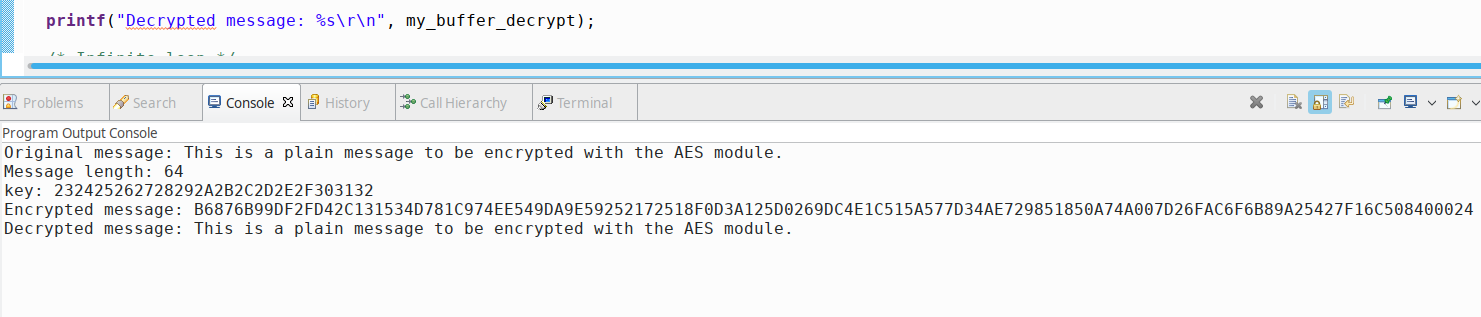
\includegraphics[width=0.95\textwidth, keepaspectratio]{imatges/AESWebCheckConsole.png}
 \caption{Consola de l'exemple AES\_1}
 \label{fig:aes_console}
\end{figure}

El resultat també el podem comprovar a una eina externa per corroborar que el procés és vàlid i compatible amb algun altre SW de xifratge/desxifratge AES-128. Podem fer servir la web {\em aes online domain tools} per comprovar-ho (\href{http://aes.online-domain-tools.com/}{link}, veure Figura~\ref{fig:aes_web}).

\begin{figure}
 \centering
 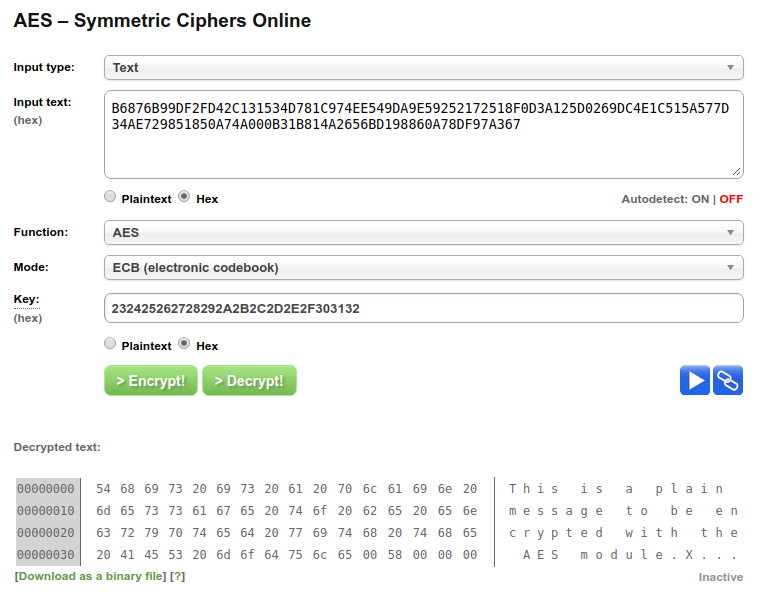
\includegraphics[width=0.85\textwidth, keepaspectratio]{imatges/AESWebCheck.png}
 \caption{Web per desxifrar el text xifrat de l'exemple AES\_1}
 \label{fig:aes_web}
\end{figure}

\chapter{Altres perifèrics}
\label{ch:otherperipherals}
Fins ara s'han introduït els perifèrics més habituals i que es poden trobar a als microcontroladors actuals. Tot i això, hi ha altres perifèrics més específics d'algun àmbit d'aplicació que no s'han presentat. En podem enumerar uns quants sense poder ser exhaustius:

\begin{itemize}
%  \item Mòduls {\em crypto} que permeten operacions de tipus criptogràfic per realitzar càlculs de claus criptogràfiques. Sovint aquesta mena de mòduls suporten directament el xifratge o desxifratge en estàndards com AES, DES, triple-DES, etc. \cite[720]{STM32F4RM}\cite[772]{STM32F4RM}\cite[453]{EFM32TGRM}.
 \item \gls{DMA} avançats, que permeten fer transferències complexes, no tant sols d'un {\em buffer} d'una sola dimensió (com els {\em arrays}) si no de dues dimensions per moure imatges o matrius de 2 dimensions \cite[339]{STM32F4RM}.
 \item {\em Drivers} \gls{LCD} que poden controlar directament pantalles \cite[480]{STM32F4RM}\cite[490]{EFM32TGRM}. Segons el model i el fabricant aquest mòdul podrà controlar diferents tipus de pantalla (LCD o TFT), amb color o blanc i negre, diferents resolucions i profunditat de color, etc.
 \item Mòdul controlador de USB que permet connectar i controlar el microcontrolador al bus USB \cite[965]{STM32F4RM}\cite[1446]{EFM32GG11RM}.
 \item Mòdul Ethernet per poder connectar el nostre sistema encastat a una xarxa cablejada amb Ethernet. Aquests tipus de perifèrics necessiten un xip extern que es controla per un bus força estandarditzat anomenat \gls{MII} (o el més modern RMII) \cite[1121]{STM32F4RM}\cite[1729]{EFM32GG11RM} \cite{wiki:rmi}.
 \item Controlador \gls{SDIO} per accedir a dispositius SDIO, majoritàriament targetes de memòria SD \cite[1019]{STM32F4RM}\cite[1670]{EFM32GG11RM}.
 \item Controlador de bus \gls{CAN} que permet connectar el dispositiu al bus CAN \cite[1076]{STM32F4RM}\cite[1899]{EFM32GG11RM} \cite{wiki:can}.
\end{itemize}

Treballar amb aquests perifèrics, tot i que no ho veurem en aquest llibre, és força similar a la resta de perifèrics que hem vist: estan mapats a memòria i tenen un conjunt de registres que permet controlar el perifèric a través de llegir i escriure aquests registres. Els fabricants proporcionen llibreries per facilitar-ne l'ús com amb la resta de perifèrics que hem vist.

Els perifèrics més complexos (per exemple USB o Ethernet) acostumen a portar associats una llibreria proporcionada pel fabricant o per tercers per poder controlar el perifèric i simplificar-ne l'ús. Així, per exemple, és habitual fer servir la llibreria LwIP per tenir funcionalitat de xarxa ({\em sockets}, TCP, UDP, IP, etc.) \cite{lwip}\cite{wiki:lwip} i que els fabricants proporcionin documentació o codi per enllaçar aquesta llibreria amb el seu perifèric.


\section{\em Peripheral Reflex System}

Un perifèric que proporciona el fabricant Silicon Labs per la seva línia EFM32 és el {\em Peripheral Reflex System} (\gls{PRS}). Aquest sistema és una mena de xarxa que permet a diferents perifèrics comunicar-se entre si sense involucrar la CPU, de manera que uns envien senyals que d'altres recullen per engegar alguna tasca \cite[135]{EFM32TGRM}. 

D'aquesta manera, és possible que un Timer enviï un senyal a la UART perquè inici una transmissió, o un GPIO engegui un Timer i permeti comptar quant de temps ha estat pitjat un botó. Tot això es fa sense que la CPU intervingui per a res, estalviant energia i simplificant el codi. Els senyals que es generen i es reben estan dins de canals, de manera que poden funcionar diferents canals simultàniament i connectar-hi diferents perifèrics sense que s'interfereixin. Aquest perifèric només es troba als dispositius de Silicon Labs i, fins al moment, cap altre fabricant inclou res de similar en els seus microcontroladors \cite{AN0025}.

\subsection{Un exemple amb PRS senzill}
En aquest exemple d'ús del \gls{PRS} el farem servir per comptar el temps que es polsa un dels botons de la placa de prototipat. Per fer-ho, configurarem el port GPIO per a que generi un senyal PRS per nivell i aquest alimenti a un dels canals del Timer 0. Quan es detecti el flanc de baixada del GPIO (es pitja el botó), el Timer començarà a comptar i quan es detecti el flanc de pujada (es deixa anar el botó) el Timer s'aturarà i llençarà una interrupció de tipus {\em Input Capture}. Al final, el que tindrem al registre {\em Capture} 0 del Timer serà el nombre de {\em ticks} que ha estat pitjat el botó 0.

La configuració del Timer és la que es veu al Llistat~\ref{PRSTimer}. Al codi es veu que es tria el canal 2 del PRS per activar l'{\em input capture} i es configura el Timer per a que s'engegui quan es rebi un flanc de baixada i s'aturi amb el flanc de pujada. També es pre-escala el rellotge per 1024, deixant-lo en $14.000.000 / 1024 = 13.617,875 Hz$.

\index{TIMER\_InitCC()}\index{TIMER\_Init()}\index{TIMER\_IntEnable()}\index{NVIC\_EnableIRQ()}
\begin{lstlisting}[style=customc,caption=Configuració del Timer i l'{\em input capture},label=PRSTimer]
static void TimerConfig(void) {
  TIMER_InitCC_TypeDef timerCCInit = {
    .eventCtrl = timerEventFalling,
    .edge = timerEdgeFalling,
    .prsSel = timerPRSSELCh2,
    .cufoa = timerOutputActionNone,
    .cofoa = timerOutputActionNone,
    .cmoa = timerOutputActionNone,
    .mode = timerCCModeCapture,
    .filter = false,
    .prsInput = true,
    .coist = false,
    .outInvert = false
  };

  TIMER_InitCC(TIMER0, 0, &timerCCInit);

  TIMER_Init_TypeDef timerInit = {
    .enable = false,
    .debugRun = false,
    .prescale = timerPrescale1024,
    .clkSel = timerClkSelHFPerClk,
    .fallAction = timerInputActionReloadStart,
    .riseAction = timerInputActionStop,
    .mode = timerModeUp,
    .dmaClrAct = false,
    .quadModeX4 = false,
    .oneShot = false,
    .sync = false
  };

  TIMER_Init(TIMER0, &timerInit);
  TIMER_IntEnable(TIMER0, TIMER_IF_CC0);
  NVIC_EnableIRQ(TIMER0_IRQn);
}
\end{lstlisting}

La configuració del pin és més senzilla, tal com es veu al Llistat~\ref{PRSGPIO}. Simplement es configura que els GPIO generaran senyals PRS i es configura el canal número 2 per que rebi el valor del pin 8.

\index{GPIO\_PinModeSet()}\index{GPIO\_IntConfig()}\index{GPIO\_InputSenseSet()}\index{PRS\_SourceSignalSet()}
\begin{lstlisting}[style=customc,caption=Configuració del GPIO per generar un senyal PRS,label=PRSGPIO]
 static void GPIOConfig(void) {
  GPIO_PinModeSet(gpioPortD, 7, gpioModePushPullDrive, 0); /* LED */
  GPIO_PinModeSet(gpioPortD, 8, gpioModeInput, 0); 		 /* Boto 0 */
  GPIO_PinModeSet(gpioPortB, 11, gpioModeInput, 0); 		 /* Boto 1 */

  /* Set Interrupt configuration for both buttons */
  GPIO_IntConfig(gpioPortD,  8, false, true, true);
  GPIO_IntConfig(gpioPortB, 11, false, true, true);

  GPIO_InputSenseSet(GPIO_INSENSE_PRS, _GPIO_INSENSE_RESETVALUE);

  PRS_SourceSignalSet(2, PRS_CH_CTRL_SOURCESEL_GPIOH, PRS_CH_CTRL_SIGSEL_GPIOPIN8, prsEdgeOff);
}
\end{lstlisting}

Per últim, el Timer està configurat per generar una \gls{IRQ} en quan capturi el valor del comptador el CC1. Per tant, cal escriure la \gls{ISR} corresponent i tractar les dades com toca. En aquest cas només es treu per la consola el valor llegit en ticks del Timer. A la funció {\bf main()} tant sols hi ha la configuració dels perifèrics, ja que un cop configurats, la CPU no cal que faci res fins que no es crida la ISR; és per això que dins el bucle principal es posa la CPU en el mode EM1 de baix consum amb la crida a la funció {\bf EMU\_EnterEM1()}\index{EMU\_EnterEM1()}.

\index{TIMER0\_IRQHandler()}\index{TIMER\_IntGet()}\index{TIMER\_IntClear()}\index{TIMER\_CaptureGet()}
\begin{lstlisting}[style=customc,caption=ISR del Timer,label=PRSISR]
void TIMER0_IRQHandler(void) {
  volatile uint32_t time_value = 0;

  uint32_t aux;
  aux = TIMER_IntGet(TIMER0);

  TIMER_IntClear(TIMER0, aux);

  time_value = TIMER_CaptureGet(TIMER0, 0);
  printf("time button 0: %lu\r\n", time_value); // 13672 ticks / second
} 
\end{lstlisting}



\subsection{Exemple amb PRS, DMA, DAC i ADC}

Anem a veure un exemple força complex, on intervindran el DMA, l'ADC, el DAC i un parell de Timers. El que farà l'exemple serà enregistrar els valors durant 2 segons d'una entrada analògica per replicar-la després per una sortida també analògica. Per això, es configurarà l'ADC per que faci les lectures i es vagin guardant a un buffer fent servir el DMA i després es faci l'operació a la inversa cap el DAC.

Per marcar el ritme de captura de l'ADC i de conversió del DAC es farà servir un senyal PRS proporcionat per Timers. D'aquesta manera, es configurarà un {\em Timer} per a que generi un senyal PRS cada cop que fa {\em overflow} i aquest senyal engegui el procés de conversió de l'ADC i un altre Timer per generar un senyal similar pel DAC.

A l'exemple es configurarà l'ADC perquè prengui mostres del canal 6 amb referencia de tota l'escala, tot seguit es configura perquè el seu {\em trigger} sigui el canal 0 del PRS (veure Llistat~\ref{DMAADCPRS}).

\index{ADC\_InitSingle()}
\begin{lstlisting}[style=customc,caption=Configuració de l'ADC perquè funcioni amb el PRS ,label=DMAADCPRS]
static void ADCConfig(void) {
  ...
  singleInit.reference = adcRefVDD;
  singleInit.input = adcSingleInpCh6;
  
  /* Use PRS channel 0 */
  singleInit.prsEnable = true;
  singleInit.prsSel = adcPRSSELCh0;
  ADC_InitSingle(ADC0, &singleInit);
  ...
}
\end{lstlisting}

A continuació es configura el canal PRS perquè sigui el Timer 0 qui generi el senyal i es configurà també el Timer 0 perquè generi un pols a la freqüència desitjada (Llistat~\ref{DMAADCTIMER}).

\index{TIMER\_Init()}\index{TIMER\_TopBufSet()}\index{PRS\_SourceSignalSet()}
\begin{lstlisting}[style=customc,caption=Configuració del Timer0 perquè funcioni amb el PRS ,label=DMAADCTIMER]
static void ADCConfig(void) {
  ...
  PRS_SourceSignalSet(0, PRS_CH_CTRL_SOURCESEL_TIMER0, PRS_CH_CTRL_SIGSEL_TIMER0OF, prsEdgeOff);

  TIMER_Init_TypeDef timerInit = TIMER_INIT_DEFAULT;
  timerInit.enable = false;
  TIMER_Init(TIMER0, &timerInit);
  TIMER_TopBufSet(TIMER0, CMU_ClockFreqGet(cmuClock_TIMER0)/SAMPLING_FREQ);
}
\end{lstlisting}

Amb això tindrem que quan s'engegui el Timer 0, aquest anirà generant senyals pel PRS que faran que l'ADC faci una conversió de senyal. Ara cal configurar el DMA perquè reculli aquesta dada i l'emmagatzemi on pertoca. Això es farà de forma molt similar a l'exemple anterior, configurant el canal de manera que la font del senyal serà l'ADC (paràmetre DMAREQ\_ADC0\_SINGLE)  i que l'origen de dades no s'ha de canviar i el destí s'ha d'incrementar de 2 en 2 (ja que llegirem dades de l'ADC de tipus uint16\_t que son de 2 bytes) (Llistat~\ref{DMAADCDMA}).

\index{DMA\_CfgChannel()}\index{DMA\_CfgDescr()}
\begin{lstlisting}[style=customc,caption=Configuració del DMA per obtenir dades de l'ADC, label=DMAADCDMA]
static void DMAConfig(void) {
  ...
  /* configure DMA for ADC reads */
  dma_cb_adc.cbFunc = dmaTransferCompleteADC;
  dma_cb_adc.userPtr = NULL;

  chnlCfg.highPri = false;
  chnlCfg.enableInt = true;
  chnlCfg.select = DMAREQ_ADC0_SINGLE;
  chnlCfg.cb = &dma_cb_adc;
  DMA_CfgChannel(DMA_CHANNEL_ADC, &chnlCfg);

  descrCfg.srcInc = dmaDataIncNone;
  descrCfg.dstInc = dmaDataInc2;
  descrCfg.size = dmaDataSize2;
  descrCfg.arbRate = dmaArbitrate1;
  descrCfg.hprot = 0;
  DMA_CfgDescr(DMA_CHANNEL_ADC, true, &descrCfg);
  ...
}
\end{lstlisting}

Per últim, per engegar aquest procés ho farem a través del botó 0 de la placa i per tant hem de posar el codi que engega el Timer 0 i que activa el DMA a la ISR corresponent (Llistat~\ref{DMAADCISR}).

\index{DMA\_ActivateBasic()}\index{TIMER\_CounterSet()}\index{TIMER\_Enable()}
\begin{lstlisting}[style=customc,caption=Configuració del DMA per obtenir dades de l'ADC, label=DMAADCISR]
void GPIO_EVEN_IRQHandler(void) {
  uint32_t aux;

  /* clear flags */
  aux = GPIO_IntGet();
  GPIO_IntClear(aux);

  LedOn();

  /* Activate DMA transfer */
  DMA_ActivateBasic(DMA_CHANNEL_ADC, true, false, (void*)DMAbufferADC, (void*)&(ADC0->SINGLEDATA), SAMPLES-1);

  /* Activate TIMER 0 */
  TIMER_CounterSet(TIMER0, 0);
  TIMER_Enable(TIMER0, true);
}
\end{lstlisting}

Un procés molt similar és el que cal fer per realitzar l'operació inversa, és a dir, fer que el DMA transfereixi les dades obtingudes cap al DAC perquè aquest generi el senyal analògic corresponent. Primer es configura el DAC indicant que cal que faci una conversió cada cop que rebi un senyal del canal PRS número 3 (Llistat~\ref{DMADAC}).

\index{DAC\_InitChannel()}
\begin{lstlisting}[style=customc,caption=Configuració del DAC perquè funcioni amb el PRS, label=DMADAC]
static void DACConfig(void) {
  ...
  /* Use PRS channel 3 */
  initChannel.prsEnable = true;
  initChannel.prsSel = dacPRSSELCh3;
  DAC_InitChannel(DAC0, &initChannel, 1); 
  ...
}
\end{lstlisting}
A continuació es configura el canal número 3 del PRS perquè obtingui el senyal del Timer 1 (Llistat~\ref{DMADACPRS}). I per últim es configura el DMA perquè el seu {\em trigger} sigui el canal 1 del DAC (Llistat~\ref{DMADACDMA}).

\index{TIMER\_Init()}\index{TIMER\_TopBufSet()}\index{PRS\_SourceSignalSet()}
\begin{lstlisting}[style=customc,caption=Configuració del PRS i el Timer, label=DMADACPRS]
static void DACConfig(void) {
  ...
  /* Configure PRS channel 3 trigger to be TIMER1*/
  PRS_SourceSignalSet(3, PRS_CH_CTRL_SOURCESEL_TIMER1, PRS_CH_CTRL_SIGSEL_TIMER1OF, prsEdgeOff);

  TIMER_Init_TypeDef timerInit = TIMER_INIT_DEFAULT;
  timerInit.enable = false;
  TIMER_Init(TIMER1, &timerInit);
  TIMER_TopBufSet(TIMER1, CMU_ClockFreqGet(cmuClock_TIMER1)/SAMPLING_FREQ);
}
\end{lstlisting}

\index{DMA\_CfgChannel()}\index{DMA\_CfgDescr()}
\begin{lstlisting}[style=customc,caption=Configuració del PRS i el Timer, label=DMADACDMA]
static void DMAConfig(void) {
  ...
  chnlCfg.highPri = false;
  chnlCfg.enableInt = true;
  chnlCfg.select = DMAREQ_DAC0_CH1;
  chnlCfg.cb = &dma_cb_dac;
  DMA_CfgChannel(DMA_CHANNEL_DAC, &chnlCfg);

  descrCfg.srcInc = dmaDataInc2;
  descrCfg.dstInc = dmaDataIncNone;
  descrCfg.size = dmaDataSize2;
  descrCfg.arbRate = dmaArbitrate1;
  descrCfg.hprot = 0;
  DMA_CfgDescr(DMA_CHANNEL_DAC, true, &descrCfg);
}
\end{lstlisting}


La ISR del botó 1, haurà d'engegar el DMA i el Timer 1 per engegar el procés de generar el senyal prèviament mostrejat (Llistat~\ref{DMADACISR}).

\index{DMA\_ActivateBasic()}\index{TIMER\_CounterSet()}\index{TIMER\_Enable()}
\begin{lstlisting}[style=customc,caption=ISR del botó 1, label=DMADACISR]
void GPIO_ODD_IRQHandler(void) {
  uint32_t aux;

  /* clear flags */
  aux = GPIO_IntGet();
  GPIO_IntClear(aux);

  /* Activate DMA transfer */
  DMA_ActivateBasic(DMA_CHANNEL_DAC, true, false, (void*) &(DAC0->CH1DATA), (void*)DMAbufferADC, SAMPLES-1);

  /* Activate TIMER 1 */
  TIMER_CounterSet(TIMER1, 0);
  TIMER_Enable(TIMER1, true);
}
\end{lstlisting}


\chapter{Una aplicació completa}
\label{ch:aplicaciosenzilla}
Ja va sent hora de fer una aplicació completa (senzilla) per il·lustrar tot el que hem anat aprenent durant el curs.

Anem a veure una \href{https://github.com/mariusmm/cursembedded/tree/master/Simplicity/Barebone_App_1}{aplicació sencera} on ajuntarem unes quantes coses de les que hem vist fins ara. Farem una aplicació que segons la proximitat de la ma al sensor (o del sensor a una taula o un obstacle), faci pampallugues més ràpid o més lent el LED de la PCB. Farem servir el sensor de proximitat APDS-9960 connectat a la nostra placa de prototipat com ja vàrem fer a l'exemple d'I2C. Per tant, caldrà anar llegint cíclicament el sensor de proximitat i canviar el valor de \gls{PWM} del LED segons el valor llegit.

Com que aquest projecte fa servir diferents perifèrics del microcontrolador i les seves llibreries, cal organitzar el codi perquè tot sigui entenedor i amb un manteniment senzill. Així, tindrem un conjunt de mòduls (se li diu mòdul a una parella de fitxers .c i .h) per manegar les diferents funcionalitats, sensors i perifèrics. Per últim, tindrem el fitxer {\em main.c} on hi ha la funcionalitat principal de l'aplicació.

\section{Biblioteques}
Aquesta aplicació fa servir quatre biblioteques per organitzar el codi, anem a descriure-les amb detall.

\subsection{BSP}
Habitualment en aquest mòdul s'hi posen les configuracions i inicialitzacions de diferents perifèrics o dispositius comuns a tot el sistema.

En aquest cas es gestiona algun dels rellotges del sistema, el pin corresponent al LED i es configura la sortida de la consola pel {\bf printf}.

D'aquesta biblioteca es fa servir la funció {\bf setupSWOForPrint()}\index{setupSWOForPrint()} i la funció {\bf BSP\_Init()}\index{BSP\_Init()}. Aquesta segona funció tant sols crida la primera i inicialitza el LED de la placa.

\subsection{I2C\_Wrapper}

Hem escrit una biblioteca senzilla per accedir al bus \gls{I2C} fent servir la llibreria emlib. D'aquesta manera encapsulem tota la funcionalitat en dues funcions senzilles de fer servir per llegir o escriure un registre d'un dispositiu I2C ({\bf I2C\_WriteRegister}\index{I2C\_WriteRegister()} i {\bf I2C\_ReadRegister}\index{I2C\_ReadRegister()}) com ja es va fer a \fullref{sub:I2C_example}.

\index{I2C\_WriteRegister()}\index{I2C\_TransferInit()}\index{I2C\_Transfer()}
\begin{lstlisting}[style=customc, caption={Part de la funció {\bf I2C\_WriteRegister}}, label=I2CWriteRegister]
bool I2C_WriteRegister(uint8_t addr, uint8_t reg, uint8_t data) {
  ...
  I2C_Status = I2C_TransferInit(I2C0, &seq);

  while (I2C_Status == i2cTransferInProgress) {
    I2C_Status = I2C_Transfer(I2C0);
  }
  ...
}
\end{lstlisting}


\subsection{PWM}
És una biblioteca molt senzilla per controlar el canal PWM que correspon al LED de la nostra placa. Només suporta aquest canal i només proporciona una funció per controlar el PWM, amb un paràmetre amb el percentatge de \gls{duty cycle} del PWM (100\% equival al LED sempre encès i 0\% correspon al LED apagat).
La funció {\bf PWM\_Init()}\index{PWM\_Init()} configura el Timer1 perquè funcioni com a generador de \gls{PWM}, de manera molt similar a l'exemple \fullref{sub:PWM_example}.

L'altra funció de la biblioteca és {\bf PWM\_Set()}\index{PWM\_Set()}, que rep el percentatge del \gls{duty cycle} que ha d'estar a 1 i configura el Timer d'acord a aquest percentatge. Com que el Timer està configurat perquè compti fins a {\bf PWM\_FREQ} (que val 4096), cal passar del rang 0 -- 100 a 0 -- 4096. Un cop calculat el valor correcte, s'usa com a valor al comparador del {\em timer}.

\index{PWM\_Set()}\index{TIMER\_CompareBufSet()}
\begin{lstlisting}[style=customc,caption={Funció PWM\_Set()},label=PWMSet]
void PWM_Set(uint8_t percentage) {
  uint32_t pwm_value;
  ...
  /* convert to percentage (0 to 100) to range 0 - PWM_FREQ */
  pwm_value = percentage * PWM_FREQ / 100;

  TIMER_CompareBufSet(TIMER1, 1, pwm_value);
}
\end{lstlisting}


\subsection{APDS-9960}
Aquesta biblioteca controla el sensor APDS-9960 via el bus \gls{I2C}. Només gestiona la funcionalitat de sensor de proximitat (que pot fer força més coses).

\index{APDS\_9960\_InitProximity()}\index{I2C\_WriteRegister()}
\begin{lstlisting}[caption={Funció {\bf APDS\_9960\_InitProximity()}},style=customc,label=InitProximity]
void APDS_9960_InitProximity() {
  // Enable Proximity detection
  // ENABLE <- 5 & 2 & 0 bits
  I2C_WriteRegister(DEVICE_ADDR, APDS_ENABLE_REG, 0x25);

  /* LED Strength to 100mA, Proximity Gain control to 8x */
  I2C_WriteRegister(DEVICE_ADDR, APDS_CTRL_1_REG, 0x0C);

  /* LED_BOOST 300% 0111_0001*/
  I2C_WriteRegister(DEVICE_ADDR, APDS_CTRL_2_REG, 0x71);
}
\end{lstlisting}

La funció {\bf APDS\_9960\_InitProximity()}\index{APDS\_9960\_InitProximity()} (Llistat~\ref{InitProximity}) inicialitza el sensor per a què funcioni com a sensor de proximitat. Cal consultar el Datasheet per veure els registres que s'escriuen i quins valors es posen \cite{apds9960}.

\index{APDS\_9960\_ReadProximity()}\index{I2C\_ReadRegister()}
\begin{lstlisting}[caption={Funció {\bf APDS\_9960\_ReadProximity()}},style=customc,label=ReadProximity]
bool APDS_9960_ReadProximity(uint8_t *p_data) {
  uint8_t status;
  bool ret = false;

  I2C_ReadRegister(DEVICE_ADDR, APDS_STATUS_REG, &status);

  if ((status & 0x02) != 0x00) {
    I2C_ReadRegister(DEVICE_ADDR, APDS_PDATA_REG, p_data);
    ret = true;
  }

  return ret;
}
\end{lstlisting}

La funció {\bf APDS\_9960\_ReadProximity()}\index{APDS\_9960\_ReadProximity()} (Llistat~\ref{ReadProximity}) llegeix el registre d'estatus i si hi ha una dada disponible la llegeix, la retorna a travès del paràmetre per referència i el retorn de la funció valdrà {\bf True}; si no hi ha una dada disponible retorna {\bf False}.

La biblioteca es basa en {\em polling} per saber si la dada a llegir és bona, comprovant el registre {\bf status} i retornant fals si no s'ha pogut llegir. Es podria millorar la biblioteca fent que el sensor llenci una interrupció cada cop que tingui una dada nova (es veurà més endavant a \fullref{sec:full_app_irq}).

\section{Funció principal}
La funció principal de l'aplicació està en el propi {\bf main()}\index{main()} i consta bàsicament d'un bucle sense fi on es va llegint el valor de proximitat del sensor (si està disponible) i s'ajusta el \gls{duty cycle} del \gls{PWM} segons aquest valor, de manera que el LED pampalluguegi més sovint quan més a prop estigui l'obstacle.

\index{APDS\_9960\_ReadProximity()}\index{PWM\_Set()}
\begin{lstlisting}[caption={Funció principal},style=customc,label=ProximityExample]
while(pdTrue) {
  ret = APDS_9960_ReadProximity(&p_data);

  if (ret == true) {
    printf("Proximity: %d\r\n", p_data);

    /* Convert from range 0 - 256 to 0 - 100 */
    PWM_Set((p_data * 100) / 256);
  }
}
\end{lstlisting}

Com que hem escrit la funció {\bf APDS\_9960\_ReadProximity()}\index{APDS\_9960\_ReadProximity()} de manera que retorni true o false segons si s'ha pogut llegir o no una dada, el codi ens queda molt senzill i llegible. Si s'ha pogut llegir, es treu per la consola de {\em debug} la dada i es converteix al rang adequat el valor llegit.

\begin{remark}
 Fixem-nos que la conversió de rang es fa forçant primer la multiplicació per 100 abans de la divisió per 256 per tal de no perdre precisió en la conversió. Com que treballem amb nombres enters, la divisió és entera i si ho féssim a l'inrevés obtindríem sempre valors 0, ja que <valor de 8 bits>/256 sempre dona 0 en una divisió entera i després encara que ho multipliquéssim per 100 seguiria donant 0..
\end{remark}


\section{Afegint-hi interrupcions}
\label{sec:full_app_irq}
En els exemples que hem vist fins ara, tant de perifèrics integrats com de dispositius externs la comunicació es feia via {\em polling}, això és, preguntant tota l'estona si el dispositiu o perifèric té alguna dada disponible. L'altre manera de comunicar-se és mitjançant interrupcions, fent que el dispositiu o perifèric llenci una \gls{IRQ} cada cop que té una dada disponible.

Per això, ens calen almenys, fer els següents canvis al nostre sistema:
\begin{itemize}
 \item Connectar el pin d'\gls{IRQ} del sensor a la nostra placa de desenvolupament
 \item Configurar el sensor {\bf APDS-9960}, de manera que generi un senyal d'IRQ cada cop que tingui una nova dada disponible
 \item Habilitar les interrupcions al nostre microcontrolador perquè cridi la \gls{ISR} corresponent.
\end{itemize}

\subsection{Connexió del pin INT}
Per aconseguir connectar el pin INT del sensor {\bf APDS-9960} només cal fer servir un cinquè cable Dupont entre la placa de prototipat del sensor i la nostra placa de desenvolupament. Si mirem el manual de la placa de Silicon Labs, veurem que el pin PB12 es pot fer servir com a un GPIO normal i que generi una interrupció cada cop que tinguem un flanc.

Segons el {\em datasheet} \cite[3]{apds9960} del APDS-9960 el pin d'interrupció és de tipus \gls{open drain}. Això vol dir que aquest pin només pot forçar un valor '0' i li cal que el valor '1' estigui forçat per un \gls{pull-up}. En el cas de la placa que tenim, ja incorpora aquesta resistència de \gls{pull-up}, per tant, el pin de GPIO del microcontrolador no cal configurar-lo com entrada amb \gls{pull-up}.
\index{GPIO\_PinModeSet()}
\begin{lstlisting}[style=customc]
GPIO_PinModeSet(gpioPortB, 12, gpioModeInput, 1); /* IRQ from APDS_9960 */
\end{lstlisting}

Si la PCB no tingues la resistència de \gls{pull-up}, caldria configurar el pin com a \gls{pull-up} ja que si no ens trobaríem que sempre estaria a '0', ja que cap dels dos dispositius el posaria a '1'.

\subsection{Configurar el dispositiu APDS{\-}9960}
Ara cal que el sensor generi un senyal d'\gls{IRQ} cada cop que tingui una nova dada disponible.
% Veiem al {\em datasheet}\cite[p.20 i 21]{apds9960} que cal activar les interrupcions per proximitat (bit PIEN de l'Status Register) i posar uns valors adients als registres de {\em threshold} (adreces 0x88 i 0x89). Segons ens diu el {\em datasheet}, si el registre {\bf PDATA} està dins del nivell que marquen aquests dos registres es generarà una interrupció. Per últim, cal configurar el valor del camp {\bf PPERS} del registre {\bf Persistence} per
Veiem al {\em datasheet} \cite[11 i 20]{apds9960} que cal activar les interrupcions per proximitat (bit {\bf PIEN} del registre {\bf Status}) i si configurem el valor del camp {\bf PPERS} del registre {\bf Persistence} al valor 0 generarà una interrupció cada cop que hi hagi una dada nova.

\index{APDS\_9960\_InitProximity\_IRQ()}\index{I2C\_WriteRegister()}
\begin{lstlisting}[caption={Nova funció d'initialització del APDS{\_}9960},style=customc,label=APDS960InitProximityIRQ]
void APDS_9960_InitProximity_IRQ() {
  //Enable Proximity detection
  // ENABLE <- 5 & 2 & 0 bits
  I2C_WriteRegister(DEVICE_ADDR, APDS_ENABLE_REG, 0x25);

  /* LED Strength to 100mA, Proximity Gain control to 8x */
  I2C_WriteRegister(DEVICE_ADDR, APDS_CTRL_1_REG, 0x0C);

  /* LED_BOOST 300% 0111_0001*/
  I2C_WriteRegister(DEVICE_ADDR, APDS_CTRL_2_REG, 0x71);

  /* Generate IRQ every data valid */
  I2C_WriteRegister(DEVICE_ADDR, APDS_PERSISTENCE_REG, 0);
}
\end{lstlisting}

Amb aquesta configuració segons el {\em datasheet} el sensor posarà una interrupció cada cop que hi hagi una dada nova disponible de proximitat.

\subsection{Habilitar la interrupció corresponent}
L'últim pas és habilitar la interrupció corresponent al pin d'entrada que hem triat. És una operació molt similar al que ja s'ha vist a l'apartat dels GPIOs (\fullref{sub:GPIO_2}).

\index{GPIO\_IntConfig()}\index{NVIC\_EnableIRQ()}
\begin{lstlisting}[caption={Habilitar l'interrupció del pin corresponent},style=customc,label=APDS960EnableIRQ]
GPIO_IntConfig(gpioPortD, 8, false, true, true);
NVIC_EnableIRQ(GPIO_EVEN_IRQn);
\end{lstlisting}

Un cop tenim tot preparat, cal també modificar la nostra funció principal perquè no faci {\em polling}, que és el que volem evitar. Com que ara tenim una {\em ISR} que s'executarà cada cop que que hi hagi una dada nova al sensor, tenim vàries opcions, en destaquem dues:
\begin{itemize}
 \item Fer la lectura del registre del sensor des de la pròpia \gls{ISR}
 \item Activar un {\em flag} que ens indiqui que podem fer la lectura des de la funció principal.
\end{itemize}

Com ja s'ha comenta anteriorment (\fullref{ch:IRQ}) posar gaire codi dins una \gls{ISR} no és aconsellable, així que per aquest exemple farem servir la segona opció proposada. Per tant, afegirem una variable de tipus {\em bool} al projecte que farem servir com a {\em flag}. Aquest {\em flag} el posarem a {\bf true} dins la \gls{ISR} i la funció principal l'esborrarà cada cop que el faci servir (Llistats~\ref{APDS960ISRFlag} i \ref{APDS960Readmain}).

\index{GPIO\_EVEN\_IRQHandler()}\index{GPIO\_IntGet()}\index{GPIO\_IntClear()}
\begin{lstlisting}[caption={\gls{ISR} amb el {\em flag}},style=customc,label=APDS960ISRFlag]
void GPIO_EVEN_IRQHandler(void) {
  /* clear flags */
  aux = GPIO_IntGet();
  GPIO_IntClear(aux);

  signal = true;
}
\end{lstlisting}
\index{main()}\index{APDS\_9960\_ReadProximity()}
\begin{lstlisting}[caption={Funció principal amb suport d'interrupcions},style=customc,label=APDS960Readmain]
main() {
  ...
  while(signal == false);
  signal = false;

  ret = APDS_9960_ReadProximity(&p_data);
  ...
}
\end{lstlisting}

El que veiem a la funció {\bf main()}\index{main()} és que el microcontrolador estarà la major part del temps esperant a que el {\em flag} es posi a {\em true} per tal de continuar i poder fer l'operació de lectura del sensor i canviar el \gls{duty cycle} del \gls{PWM} del \gls{LED}. Tota aquesta estona que el microcontrolador està esperant-se sense poder fer res, es podrà aprofitar per posar-lo en algun mode de baix consum tal com veurem al \fullref{ch:low-power}.


%----------------------------------------------------------------------------------------
% 4a Part: FreeRTOS
%----------------------------------------------------------------------------------------s
\part{FreeRTOS}
\label{part:freertos}
%% Capitol 4
% \part{FreeRTOS}
% \label{part:freertos}
\chapter{Conceptes bàsics de FreeRTOS}
\label{ch:FreeRTOS}
% \chapter{Sistemes Operatius de Temps Real}

En el Firmware per sistemes encastats que hem vist fins ara es basen en un bucle infinit on es van executant les tasques a fer. Això acostuma a ser prou bo per sistemes senzills, com ara llegir d'un \gls{ADC} i decidir alguna cosa, o actuar sobre una sortida segons el valor d'un sensor, etc.

Per sistemes més complexos o amb requeriments crítics, s'acostuma a fer servir un Sistema Operatiu per gestionar diferents tasques.
\begin{remark}

Un sistema és de Temps Real quan el temps de resposta del sistema a un event extern està fitada. És a dir, es pot saber i està garantit el temps total entre que
succeeix un esdeveniment i el sistema genera una sortida.

Un exemple típic és el d'un airbag. El temps màxim, sigui el que sigui que el sistema estigui fent entre que es detecta l'accident i es dispara l'airbag està garantit i limitat.

Un Sistema Operatiu de Temps Real (RTOS en anglès) és un Sistema Operatiu que està dissenyat per garantir aquesta fita de temps.
\end{remark}
\glsreset{RTOS}
En aquest llibre farem servir \gls{FreeRTOS} \cite{freertos}, un \gls{RTOS} de codi obert àmpliament utilitzat. En el cas de EFM32 i STM32 els fabricants ens proporcionen el {\em porting} de FreeRTOS a les seves plataformes.

\begin{remark}
 Se'n diu {\em porting} al fet d'adaptar un codi a una plataforma específica. Per exemple, en el cas del FreeRTOS, cal adaptar una sèrie de funcions per a que tot el sistema funcioni, com ara la gestió dels rellotges, la gestió de tasques, etc.
\end{remark}


En tot \gls{OS} (i \gls{RTOS}) les feines a fer per part del sistema es reparteixen en diferents tasques (\glspl{task} en anglès). Aquestes tasques s'executen “simultàniament” i, per tant, cal repensar bé tot el sistema abans de començar a escriure el codi.

En sistemes encastats, un SO (o RTOS) no ofereix totes les funcionalitats a les que estem acostumats quan sentim parlar d'un SO. Així, normalment el que ens ofereix un RTOS és:

\begin{itemize}
 \item Gestió de tasques: Creació, execució, estat de les tasques, prioritats de tasques, etc.
 \item Comunicació entre tasques: Semàfors, cues, etc.
 \item Gestió de temps: Timers, {\em timeouts}, {\em delays}, etc.
\end{itemize}

Les tasques són les unitats bàsiques de funcionament i és on s'implementen les funcionalitats del sistema.

\section{Tasques}

Una tasca és el que es coneix com a procés en els Sistemes Operatius de propòsit general. Per tant, una tasca serà l'estructura mínima de codi en que es divideix una aplicació. Aquestes tasques seran les que el planificador o {\em scheduler} del Sistema Operatiu anirà executant i retirant d'execució segons certes condicions que veurem a continuació.

Bàsicament una tasca pot estar en l'estat {\em Running} (executant-se), {\em Ready} (disponible per ser executada) o {\em Blocked} (no preparada perquè està esperant a algun esdeveniment)\footnote{També hi ha l'estat {\em Suspended} on la pròpia tasca demana sortir de la llista de {\em Ready}}. A la Figura~\ref{fig:taskstate} es pot veure quins estats pot tenir una tasca en FreeRTOS \cite[92]{FreeRTOSBook}.


\begin{figure}
 \centering
 \fbox{\color{ocre}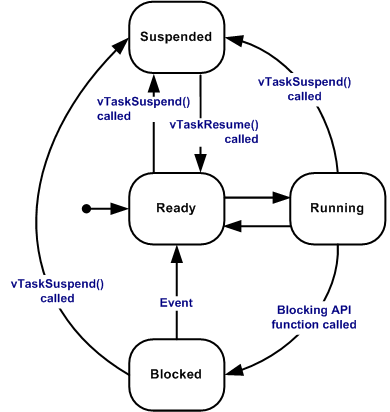
\includegraphics[width=0.85\textwidth, keepaspectratio]{imatges/tskstate.png}}
 \caption{Estats possibles d'una tasca. \copyright\ FreeRTOS}
 \label{fig:taskstate}
\end{figure}

Les tasques són funcions amb un bucle infinit i una inicialització prèvia i en cap cas la funció pot retornar. Si una tasca ja no és necessària, es pot eliminar per part el RTOS, però no pot acabar retornant la funció per si mateixa.
Pel cas de \gls{FreeRTOS}, tenen l'aspecte que es mostra al Llistat~\ref{task}.

\index{OneTask()}
\begin{lstlisting}[caption={Esquelet d'una tasca},style=customc,label=task]
static void OneTask(void *pParameter) {
  (void) pParameter;
  /* Init */

  while(1) {
    /* bucle infinit */
  }
}
\end{lstlisting}

Una aplicació basada en un RTOS és un conjunt de tasques funcionant concurrentment i comunicades entre elles. El \gls{RTOS} ens dona diferents funcions que ens permeten: comunicar tasques entre elles o bloquejar-se per un cert temps.

\subsection{Prioritats}

Quan es creen les tasques, a cada una se li assigna una certa prioritat. Aquesta prioritat marcarà quina de les tasques de l'estat {\em Ready} passarà a executar-se {\em Running} a cada moment. A \gls{FreeRTOS} les tasques amb una prioritat d'un valor més baix tenen menor prioritat (0 és el valor més baix i menys prioritari). Diferents tasques poden tenir la mateixa prioritat.

Existeix una tasca {\em Idle} que s'executa cada cop que cap altra tasca està a l'estat {\em Ready}. Aquesta tasca té la prioritat més baixa, de valor 0 i per tant només s'executa quan cap tasca està llesta. La tasca {\em Idle} sempre està disponible per executar-se a qualsevol moment.

Per saber més sobre prioritats i com assignar-les a les tasques, veieu \fullref{sec:priorities_RMA}.
\subsection{L'ús de l'{\em stack} en un S.O.}
\label{sub:StackOS}
Per crear una tasca, un dels paràmetres que es passa a la funció {\bf xTaskCreate}\index{xTaskCreate()} és la mida de l'\gls{stack} per la tasca que s'està creant.

Se'n diu {\em stack} a la regió de memòria assignada a una tasca que s'utilitza bàsicament per dues coses:
\begin{itemize}
 \item guardar els valors dels paràmetres de les diferents crides a funcions que faci la tasca
 \item emmagatzemar el seu context quan el SO retira la tasca d'execució.
\end{itemize}

Aquest \gls{stack} normalment es gestiona com una pila (amb els mètodes {\em push} i {\em pop}) i acostuma a situar-se al final de la memòria i “créixer cap avall”.

A priori, és molt difícil saber quant {\em stack} farà servir una tasca, així que el més habitual és donar un valor per defecte prou gran i després, durant el funcionament normal, observar quanta se'n fa servir realment.

Per saber el nivell màxim a on s'ha arribat a l'{\em stack} de cada tasca, FreeRTOS fa servir un mètode una pel peculiar: a l'inicialitzar la tasca (i el seu {\em stack}) omple l'{\em stack} amb un valor predeterminat i conegut. Després, quan ja està funcionant el nostre sistema, només cal comptar quantes posicions de l'{\em stack} mantenen el valor conegut. Si s'acosta a 0 voldrà dir que la tasca està fent servir la majoria de l'espai de l'{\em stack}.

Per activar aquesta funcionalitat cal editar el fitxer {\bf FreeRTOSConfig.h} i definir la macro {\bf configCHECK\_FOR\_STACK\_OVERFLOW} amb el valor 2 i la macro {\bf uxTaskGetStackHighWaterMark} a 1.

Activant la primera de les macros, el sistema operatiu també controla que no s'intenti accedir fora de l'{\em stack}. D'aquesta manera podem saber si cal més {\em stack}, però no si ens en sobra ni quanta. En activar aquesta opció cal definir una funció de hook que s'anomeni {\bf vApplicationStackOverflowHook()}\index{vApplicationStackOverflowHook()} i que es cridarà cada cop que es detecti un error en accedir l'{\em stack}.

%\section{Scheduler}

% {\bf taskYIELD()}\index{taskYIELD()}


\section{El temps en un RTOS}
\label{sec:RTOS_time}
Habitualment un RTOS ha de portar un control del temps per decidir quina tasca s'ha d'executar, saber quan desbloquejar una tasca, etc.

Normalment es basen en el concepte de \gls{tick}. Un {\em tick} es genera de forma periòdica (normalment fent servir algun Timer) i la freqüència d'aquest {\em tick} ens marca el temps mínim que pot manegar el RTOS.

En el cas de FreeRTOS, a cada {\em tick} es deixa d'executar la tasca que està {\em running} i s'executa el planificador del RTOS. Si aquest planificador detecta que una tasca més prioritària està a punt per ser executada (estat {\em ready}), la posarà a executar ({\em running}) enlloc de la que hi havia fins feia un moment.

La freqüència d'aquest {\em tick} pot variar molt segons el sistema que tinguem, però acostuma a anar entre els 1000 Hz i els 50Hz. Segons la freqüència del {\em tick} tindrem un sistema més ràpid de resposta en segons quins casos a canvi d'alentir lleugerament l'execució general del sistema i de tenir menys resolució en les funcions de control de temps.

\subsection{Funcions per controlar el temps}

Tot OS proporciona una sèrie de funcions per gestionar el temps, això és:
\begin{itemize}
 \item bloquejar una tasca durant un cert temps determinat.
 \item controlar el {\em timetout} a certes crides del mateix.
\end{itemize}

\subsubsection{\em Delays}
Les funcions {\bf vTaskDelay()}\index{vTaskDelay()} i {\bf vTaskDelayUntil()}\index{vTaskDelayUntil()} són les dues funcions que ens permeten bloquejar la tasca que la crida durant el temps que s'especifica com a paràmetre.

Aquestes dues funcions faran que la tasca entri immediatament a l'estat {\em blocked} i restarà en aquest estat durant tota l'estona que s'especifiqui. Un cop hagi passat aquest temps la tasca passarà a l'estat {\em Ready}.

El paràmetre que rep la funció {\bf vTaskDelay()}\index{vTaskDelay()} és el nombre de {\em ticks} que es vol que la tasca estigui {\em blocked}. Com més precís sigui el {\em tick} del sistema (més freqüència) més acurat podrà ser aquest {\em delay}.

Cal veure que segons la prioritat de la tasca en qüestió i de la prioritat de la tasca que s'estigui executant, aquesta tasca pot romandre en l'estat {\em Ready} un temps indefinit.

\subsubsection{\em Timeout}
A les funcions d'accedir a un recurs compartit, com un semàfor o una cua, apareix un paràmetre que és el temps (en {\em Ticks}) que la tasca que accedix esperà a poder realitzar l'operació. Així, si s'especifica un temps de 100 mil·lisegons per llegir d'una cua, la funció retornarà passat aquest temps si la cua està buida i ningú hi ha escrit res o retornarà tant bon punt algú hi escrigui alguna dada.

\section{Interrupcions en FreeRTOS}
\label{ch:FreeRTOSIRQ}

FreeRTOS deixa el maneig de les interrupcions a mans del desenvolupador, demanant unes certes condicions.

Cal tenir en compte que les interrupcions són esdeveniments totalment asíncrons i imprevisibles i que prenen el control de forma automàtica. Això fa que mentre està funcionant una \gls{ISR} el {\em kernel} del Sistema Operatiu no es pot executar i que, quan acabi d'executar la ISR, si no fem res, tornarà el control cap a la tasca que s'estava executant. Això pot provocar que una ISR alliberi un recurs o posi disponible una dada i que una tasca d'alta prioritat passi a l'estat {\em Ready} però el {\em kernel}, com que no s'executa, no pugui passar-li l'execució i se segueixi amb la taca menys prioritària que s'estava executant.

Per això les funcions per accedir a recursos com semàfors o cues des d'una \gls{ISR} tenen un paràmetre extra, que informa si s'ha despertat una tasca més prioritària. Si és el cas, cal que el codi de la ISR faci un {\bf portYIELD\_FROM\_ISR()}\index{portYIELD{\_}FROM{\_}ISR()} per cridar al {\em kernel} del Sistema Operatiu (veure Llistat~\ref{ISRYield}).

\index{any{\_}IRQHandler()}\index{xSemaphoreGiveFromISR()}\index{portYIELD{\_}FROM{\_}ISR()}
\begin{lstlisting}[style=customc,caption=Codi ISR d'exemple,label=ISRYield]
void any_IRQHandler(void) {
  BaseType_t xHigherPriorityTaskWoken = pdFALSE;

  ...
  /* Toggle semaphore */
  xSemaphoreGiveFromISR(semaphore_button_0, &xHigherPriorityTaskWoken);

  portYIELD_FROM_ISR(xHigherPriorityTaskWoken);
}
\end{lstlisting}

Aquesta funció de {\em yield} retorna de la ISR i executa el {\em kernel} si la variable passada té un valor diferent a {\bf pdFALSE}.


Sempre es diu que les \glspl{ISR} han de ser el més curtes possibles, això és pels següents motius:
\begin{itemize}
 \item Mentre s'està executant una \gls{ISR} no es pot executar cap tasca, per molt prioritària que sigui.
 \item Depenent de l'arquitectura, mentre s'està executant una ISR la resta d'\glspl{IRQ} estan desactivades.
 \item Algunes arquitectures poden permetre anidar interrupcions, cosa que augmenta la complexitat i la incertesa de tot el sistema. Quan més curta sigui la ISR més improbable que això passi.
\end{itemize}

És per això que les bones pràctiques diuen que el codi dins una \gls{ISR} hi hagi poc codi i es facin servir semàfors o cues per notificar tasques on s'executin les operacions pertinents amb les prioritats adequades.

\chapter{Primer exemple amb FreeRTOS}
\label{sec:FreeRTOS_exemple_1}
El \href{https://github.com/mariusmm/cursembedded/tree/master/Simplicity/FreeRTOS_Blink}{primer exemple} és el nostre vell conegut ‘Hello World' per embedded, és a dir, blinkar un LED.

L'exemple consisteix en una sola tasca que s'encarrega de blinkar el LED. Com totes les tasques, consisteix en un bucle infinit on s'inclou tota la funcionalitat de la tasca (Llistat \ref{HelloWorldFreeRTOSTask}).

\index{TaskLedToggle()}\index{LedToggle()}\index{vTaskDelay()}
\begin{lstlisting}[caption={Tasca TaskLedToggle per FreeRTOS},style=customc,label=HelloWorldFreeRTOSTask]
static void TaskLedToggle(void *pParameter) {
  (void) pParameter;

  for (;;) {
    LedToggle();
    vTaskDelay(pdMS_TO_TICKS(500));
  }
}
\end{lstlisting}

Aquesta tasca fa servir una funció del RTOS ({\bf vTaskDelay()}\index{vTaskDelay()}) que bloqueja la tasca per un determinat temps. Així doncs, aquesta tasca tant sols farà Toggle al LED cada mig segon. Cal fixar-se que aquesta funció rep com a paràmetre el nombre de {\em ticks} a esperar-se. Aquest número es calcula amb la macro {\bf pdMS\_TO\_TICKS()}\index{pdMS\_TO\_TICKS()}, que passa de mil·lisegons a {\em ticks}.

Al {\bf main()}\index{main()} el que veiem és que, després de la inicialització habitual hem de crear les tasques que tingui el nostre sistema i tot seguit engegar el FreeRTOS (Llistat \ref{HelloWorldFreeRTOSMain}).

\index{main()}\index{xTaskCreate()}\index{vTaskStartScheduler()}
\begin{lstlisting}[caption={Main HelloWorld per FreeRTOS},style=customc,label=HelloWorldFreeRTOSMain]
main() {
  ...
  /* Create our first task */
  xTaskCreate(TaskLedToggle, (const char *) "LedToggle",
        configMINIMAL_STACK_SIZE, NULL, TOGGLE_TASK_PRIORITY, NULL);

  /* Start FreeRTOS Scheduler */
  vTaskStartScheduler();
  ...
}
\end{lstlisting}

La funció {\bf xTaskCreate()\index{xTaskCreate()}} rep diferents paràmetres:
\begin{enumerate}
 \item Punter a la funció que implementa la tasca
 \item Nom que li posem a la tasca (per debug)
 \item \gls{stack} reservat per la tasca (veure~\fullref{sub:StackOS})
 \item Punter a paràmetres per la tasca
 \item Prioritat de la tasca
 \item {\em Handle} a la tasca creada
\end{enumerate}

Aquesta funció retorna {\bf pdPASS} si s'ha creat la tasca o un error en cas contrari.

La funció {\bf vTaskStartScheduler()\index{vTaskStartScheduler()}}, que en condicions normals no retorna mai, comença l'execució del FreeRTOS i aquest, al seu torn, executarà la nostra tasca.

% A continuació veurem diversos exemples de com comunicar tasques fent servir semàfors, mutex i cues.

% \chapter{Tasques a S.O.}




%%%%%%%% AMPLIAR

\chapter{Comunicació entre tasques}

En aquest capítol es detallen diferents mecanismes de sincronització i comunicació entre tasques en un Sistema Operatiu encastat.

Qualsevol RTOS que porti aquest nom ens oferirà una sèrie de mecanismes per a comunicar tasques entre elles. Els mecanismes més habituals són:
\begin{itemize}
 \item Semàfors: Una tasca no pot agafar un semàfor fins que una altre no l'allibera.
 \item Cues: Permeten enviar informació d'una tasca a una altra.
 \item {\em Mutex}: Permet protegir un recurs compartit de manera que només una tasca el faci servir en un moment donat.
\end{itemize}

N'hi ha d'altres, com esperar i enviar esdeveniments o grups d'esdeveniments, {\em mailboxes}, senyals, etc. que acostumen a ser pròpies de cada \gls{OS} concret.

\section{Semàfors}
Un semàfor és un dels mecanismes de comunicació entre tasques mes habituals dels que ofereix un OS. En essència el funcionament d'un semàfor és tal que una tasca prova d'agafar el semàfor i es quedarà esperant que una altra tasca doni el semàfor o ho tornarà a provar més endavant \cite[244]{EmbeddedDictionary} \cite[187]{programmingembedded}.

Habitualment es fan servir per sincronitzar almenys dues tasques que comparteixen el semàfor o per protegir una secció crítica.

\subsection{Semàfors a FreeRTOS}
A FreeRTOS tenim diferents tipus de semàfors:

\begin{itemize}
 \item {\em Binary}: pot tenir només l'estat ‘agafat' o ‘donat'. Es fan servir per sincronitzar tasques.
 \item {\em Counting}: s'emmagatzema un número, que s'incrementa en ‘donar' el semàfor i es redueix en ‘agafar' el semàfor. Sempre que tingui un valor positiu es podrà ‘agafar' el semàfor. Serveix per portar un compte del nombre de recursos disponibles.
 \item {\em Mutex}: són una variant dels semàfors binaris que inclouen mecanismes d'herència de prioritats. Es fan servir per implementar l'exclusió mútua. En parlarem més endavant, a \fullref{sec:Mutex}.
\end{itemize}

\subsection{Exemple amb semàfors}
\label{sub:semafors_exemple}
A \href{https://github.com/mariusmm/cursembedded/tree/master/Simplicity/FreeRTOS_Semaphore}{l'exemple} hi ha una tasca que es queda esperant a agafar un semàfor i quan l'aconsegueix fa un {\em toggle} del LED (Veure Llistat~\ref{semaphore_task_example}).

\index{TaskLedToggle()}\index{xSemaphoreTake()}\index{LedToggle()}
\begin{lstlisting}[style=customc,caption=Tasca amb semàfor d'exemple,label=semaphore_task_example]
static void TaskLedToggle(void *pParameter) {
  (void) pParameter;

  for (;;) {
    xSemaphoreTake(semaphore_button_0, portMAX_DELAY);
    LedToggle();
  }
}
\end{lstlisting}

La funció {\bf main()}\index{main()} crida la funció {\bf BSP\_Init()}\index{BSP{\_}Init()} que configura els GPIOs corresponents als botons i es registra una \gls{ISR} ({\bf GPIO\_EVEN\_IRQHandler()}\index{GPIO{\_}EVEN{\_}IRQHandler()}) pel botó 0, que ‘dóna' el semàfor en quan es prem el corresponent botó a la PCB (Llistat~\ref{ISR_semaphore}).

Després es crea el semàfor que compartiran la tasca i la ISR i tot seguit es crea la tasca com ja hem vist a l'exemple anterior..
Per últim s'engega el {\em kernel} del RTOS.

Cal notar que les funcions per agafar o donar un semàfor són diferents segons estiguem a una tasca o a una \gls{ISR}. En el cas de la ISR, la funció de donar al semàfor ens indica si hi ha alguna tasca que cal desbloquejar perquè l'està esperant. En cas que sigui cert, cal fer un {\em yield} des de la \gls{ISR} per a que el planificador ({\em scheduler}) del RTOS pugui actuar immediatament.

\index{xSemaphoreGiveFromISR()}\index{portYIELD{\_}FROM{\_}ISR()}
\begin{lstlisting}[caption=ISR del botó 0,style=customc,label=ISR_semaphore]
ISR() {
  ...
  /* Toggle semaphore */
  xSemaphoreGiveFromISR(semaphore_button_1, &xHigherPriorityTaskWoken);
  portYIELD_FROM_ISR(xHigherPriorityTaskWoken);
}
\end{lstlisting}

Tant en aquest exemple com en els següents el {\em timeout} de les crides és {\bf portMAX\_DELAY}. Aquesta macro serveix per indicar a la funció que es vol esperar un temps infinit a que l'operació es pugui realitzar. En aquest cas, la funció cridada no retornarà fins que pugui executar l'acció i bloquejant la tasca el temps necessari. D'aquesta mena de crides a funcions se'n diu crides bloquejants.

\begin{exercise}
Es pot provar d'implementar un codi que blinki el LED tantes vegades com vegades s'ha premut el botó 0. És pot fer amb un semàfor tipus {\em counting semaphore}.
\end{exercise}


\section{Cues}
\label{sec:queue}
Hem vist que els semàfors són útils per sincronitzar tasques i per protegir zones d'exclusió mútua, però no ens donen cap solució senzilla per enviar informació o dades d'una tasca a una altra. Aquesta comunicació és per les cues \cite[102]{FreeRTOSBook}.

Ens podem imaginar una cua com un recurs compartit entre dues o més tasques, on unes poden escriure-hi i d'altres hi poden llegir dades. Habitualment (en FreeRTOS és així), les cues s'implementen amb una estructura tipus FIFO (First-In First-Out) protegida de tal manera que no hi hagi cap \gls{race condition} durant el seu funcionament\footnote{S'anomena {\em race condition} al malfuncionament d'un codi donat que està executant-se en un entorn multitasca. Aquesta mena d'errors poden ser molt difícils de detectar i arreglar}.

A més, per tal de poder implementar sistemes d'una forma senzilla, els accessos a les cues poden ser bloquejants: la tasca que fa l'accés es quedarà bloquejada fins que pugui fer l'accés (esperar a poder escriure una dada, donat que no podia perquè la cua era plena) o esperar fins que hi hagi una dada (perquè s'ha intentat llegir de la cua quan aquesta era buida).

Les operacions habituals a una cua son:
\begin{itemize}
 \item Crear una cua ({\em create}): normalment cal especificar quin tipus de dades ha d'emmagatzemar la cua i quants espais o llocs cal preparar.
 \item Inserir una dada ({\em send}): afegir (si hi ha lloc) una dada nova a la cua.
 \item Llegir dada ({\em receive}): treure una dada (si n'hi ha) de la cua.
\end{itemize}

Altres operacions poden ser:
\begin{itemize}
 \item Mirar si hi ha una dada disponible (sense llegir-la) ({\em peek}).
 \item Esborrar tot el contingut de la cua ({\em reset}).
 \item Inserir una dada al principi de la cua (sense complir que la cua és una FIFO).
\end{itemize}

Les cues són recursos que poden ser compartits per vàries tasques, podent-hi escriure diferents tasques o \glspl{ISR} i poder llegir-la també diferents tasques, tot i que això de tenir múltiples tasques llegint d'una cua no és gaire habitual.

Per saber quina mida han de tenir les cues, veieu \fullref{sec:mida_cues}.
\subsection{Exemple amb cues}
\label{sub:cues_exemple}
A \href{https://github.com/mariusmm/cursembedded/tree/master/Simplicity/FreeRTOS_Queue}{l'exemple de cues} hi ha una sola tasca que fa {\em blinkar} el \gls{LED} segons una variable. Aquesta variable s'obté de llegir (o intentar-ho) una cua. Aquesta cua (anomenada {\em queue\_buttons}) l'escriuen les dues \gls{ISR} associades als dos botons. Una envia el valor corresponent a 250 ms i l'altre ISR envia el valor que correspont a 1000 ms (Llistat~\ref{Queue_example_ISR}).

\index{xQueueSendFromISR()}\index{portYIELD{\_}FROM{\_}ISR()}
\begin{lstlisting}[style=customc, label=Queue_example_ISR, caption=Part del codi d'una de les ISRs]
...
/* Send the data to the Queue */
xQueueSendFromISR(queue_buttons, (void* ) &new_delay,
		&xHigherPriorityTaskWoken);

/* Awake a task ? */
portYIELD_FROM_ISR(xHigherPriorityTaskWoken);
...
\end{lstlisting}


En aquest cas, la tasca fa servir la funció {\bf xQueueReceive()}\index{xQueueReceive()} amb un valor de 0 a l'últim paràmetre, que és el temps en {\em ticks} que ha d'esperar-se a rebre un valor en el cas que la cua estigui buida (veure Llistat~\ref{queue_example_main}).

\index{xQueueReceive()}\index{vTaskDelay()}\index{LedToggle()}\index{TaskLedToggle()}
\begin{lstlisting}[style=customc,label=queue_example_main, caption=Part principal de la tasca TaskLedToggle]
for (;;) {
  /* try to get new delay time from queue */
  if (xQueueReceive(queue_buttons, &recv_delay, (TickType_t ) 0)) {
    my_delay = recv_delay;
  }

  /* wait for m_delay & toggle the LED */
  vTaskDelay(my_delay);
  LedToggle();
}
\end{lstlisting}

En aquest exemple volem que encara que no hi hagi dada a la cua, la tasca segueixi executant-se. Per saber si la funció de rebre dades ha obtingut una dada nova, cal comprovar si ha retornat \gls{pdTRUE}. Si retorna \gls{pdFALSE} és que ha acabat el temps d'espera (en el nostre cas 0 {\em ticks}) i no ha pogut extreure un nou valor de la cua. Aquest és un exemple d'accés no bloquejant a una cua.

Les cues cal crear-les abans d'utilitzar-les cridant a la funció {\bf xQueueCreate()}\index{xQueueCreate()}. Aquesta funció crea la cua amb la longitud desitjada i amb la capacitat indicada (Llistat~\ref{queue_example_create}).
Usualment això es crea a la funció {\bf main()}\index{main()} o, en tot cas, abans d'engegar el Sistema Operatiu.

\index{xQueueCreate()}
\begin{lstlisting}[style=customc, label=queue_example_create, caption=Creació d'una cua]
/* Create Queue */
queue_buttons = xQueueCreate(QUEUE_LENGTH, sizeof(uint32_t));
\end{lstlisting}

% A les cues de FreeRTOS hi ha una particularitat que cal tenir en compte, i és que les funcions que accedeixen a la cua treballen amb punters a les dades, no amb les dades mateixes. Això es fa per evitar còpies de les dades innecessàries a l'stack (ho veurem més endavant).
%
% Per això a l'exemple tenim:
% \begin{lstlisting}[style=customc,label=ISR_semaphore]
%  xQueueSendFromISR(queue_buttons, (void* ) &new_delay,
%    &xHigherPriorityTaskWoken);
% \end{lstlisting}
%
% on new_delay està definit de tipus uint32_t.
%
% Això vol dir que la variable on es guarden les dades que s'envien per la cua cal que segueixi viva fins que la tasca que rep la dada pugui llegir-la. Així, cal vigilar amb variables automàtiques:

\section{Mutex}
\label{sec:Mutex}
Quan tenim un recurs, {\em driver}, memòria compartida, secció crítica o qualsevol altre recurs que només es pot fer servir per una sola tasca a cada moment, cal muntar un mecanisme d'exclusió mútua que ens asseguri que no tindrem cap problema \cite[244]{FreeRTOSBook}.

Aquest mecanisme és molt similar a un semàfor binari però cal incloure algun mecanisme per prevenir la inversió de prioritats. Aquest mecanisme és el Mutex (d'aquí els ve el nom: {\em Mutual Exclusion}). Els Mutex implementen un mecanisme d'herència de prioritats de tal manera que si una tasca d'alta prioritat està esperant un Mutex que té una tasca de baixa prioritat, aquesta última veu augmentada la seva prioritat a la mateixa prioritat que la tasca d'alta prioritat mentre té el Mutex per tal que tingui més oportunitat d'alliberar-lo ja que altres tasques amb prioritats entre mig poden bloquejar la tasca de baixa prioritat \footnote{Aquest problema és el conegut {\em inversió de prioritats} que pot donar molts mal de caps si no es detecta a temps} (veure \fullref{sec:priorityinv} més endavant).

Per l'ús correcte d'un Mutex, el que es fa és provar d'agafar el Mutex abans d'entrar a la secció crítica, si es té èxit s'executa el que calgui dins la secció crítica i a continuació s'allibera el Mutex. Com ens podem imaginar, cal que el temps que estem dins una secció crítica sigui el més curt possible. Com la resta de crides d'aquesta mena, el paràmetre {\em timeout} ens permet seleccionar el temps que la tasca ha d'estar esperant auqe el Mutex estigui disponible (des de 0 fins a temps infinit).

En el cas de FreeRTOS cal primer crear el Mutex i a partir de llavors ja es pot fer servir per part de les tasques. Les tasques poden agafar o donar un Mutex amb les mateixes funcions de manegar semàfors que ja coneixem.



\subsubsection{Exemple amb Mútex}
\label{sub:mutex_exemple}
Al \href{https://github.com/mariusmm/cursembedded/tree/master/Simplicity/FreeRTOS_Mutex}{repositori del curs} tenim un exemple on dues tasques fan ús d'un recurs compartit com pot ser la consola de debug (amb el printf) i es comparteix amb un Mutex.

A l'exemple tal com està ara, no està definit la macro USE\_MUTEX i el codi no en fa ús. Si executem el codi tal qual està, veurem que la sortida de les dues tasques es barreja ja que no hi ha cap control de qui escriu i quan (Llistat \ref{outputconsole_1}).

\index{xSemaphoreTake()}
\begin{lstlisting}[style=customc, numbers=left, caption=Exemple d'ús de macros en C, label=macro_example]
#ifdef USE_MUTEX
  if (xSemaphoreTake(example_mutex, portMAX_DELAY)) {
#else
  {
#endif
\end{lstlisting}

\begin{remark}
 Un exemple d'ús de macros en C es veu al llistat~\ref{macro_example}. En aquest codi, si la macro {\bf USE\_MUTEX} no està definida no s'executa la línia 2 i no es té en compte el Mutex.
\end{remark}


\begin{lstlisting}[style=customc, label=outputconsole_1, caption=Sortida de la consola sense Mutex]
from Task1
Other text Some text from Task 2
from Task1
Other text Some text from Task 2
from Task1
Other text Some text from Task 2
from Task1
\end{lstlisting}

Si traiem el comentari i activem la macro USE\_MUTEX llavors el codi de manegar el Mutex s'activa i llavors veurem que la sortida per la consola ja és la correcta (Llistat~\ref{outputconsole_2}).
\begin{lstlisting}[style=customc, label=outputconsole_2, caption=Sortida de la consola amb Mutex]
Some text from Task1
Other text from Task 2
Some text from Task1
Other text from Task 2
Some text from Task1
Other text from Task 2
\end{lstlisting}

Què passa en aquest cas? Doncs que abans de treure el text per la consola, es demana el Mutex i queda protegida la secció crítica i tot funciona com ha de ser.

A l'exemple es fa servir la comanda {\bf taskYIELD()}\index{taskYIELD()} entre mig dels dos printf per simular que la tasca en aquell punt perd l'execució. Com segur que saps, les condicions de carrera (\glspl{race condition}) són molt complicades de trobar i provocar perquè són infreqüents i només passen de tant en tant; i és per això que provoquem el canvi de tasca amb la comanda {\bf taskYIELD()}.

En aquest exemple i per fer-ho senzill, la crida per demanar el Mutex porta com a segon paràmetre {\bf portMAX\_DELAY}, que fa que la tasca quedi bloquejada fins que s'alliberi el Mutex. També es pot afegir un temps d'espera ({\em timeout}) i llavors la funció retorna quan s'ha agafat el Mutex (i retorna \gls{pdTRUE}) o quan ha passat el temps d'espera (i retorna \gls{pdFALSE}).

L'ús de Mútex és necessari per controlar l'accés a qualsevol secció crítica que tinguem al nostre projecte. Habitualment en tindrem per cada ús o crida a un {\em driver} que pugui portar-nos problemes d'aquesta mena. Per exemple, si dues tasques han d'accedir al bus \gls{I2C} per accedir a diferents sensors caldrà protegir amb un Mutex les crides a les llibreries del sistema.

\begin{exercise}
La prioritat de les dues tasques a l'exemple és la mateixa. Com exercici es pot provar de canviar les prioritats i treure els Mutex, a veure què passa i intentar entendre el perquè.
\end{exercise}

\chapter{Exemple amb la UART i interrupcions}
A l’\href{https://github.com/mariusmm/cursembedded/tree/master/Simplicity/FreeRTOS_UART}{exemple Freertos\_UART} hi ha el mateix exemple vist a \fullref{sec:UART_example_2} però en aquest cas usant FreeRTOS. Per això hi ha uns pocs canvis:
\begin{itemize}
 \item A les interrupcions de la USART ({\bf USART1\_TX\_IRQHandler()}\index{USART1{\_}TX{\_}IRQHandler()} i {\bf USART1\_RX\_IRQHandler()}\index{USART1{\_}RX{\_}IRQHandler()}) se les canvia la prioritat, ja que a FreeRTOS la prioritat de les interrupcions han de tenir un valor diferent a 0. Veure aquest enllaç de la documentació de FreeRTOS \cite{FreeRTOSIRQ}.
 \item Enlloc de fer servir el \gls{buffer circular} es fa servir una cua de FreeRTOS. Així la \gls{ISR} de recepció guarda el valor rebut a una cua i la \gls{ISR} de transmissió va buidant la mateixa cua.
 \item La funció {\bf USART\_Send()}\index{USART{\_}Send()} també fa servir la cua de transmissió per extreure els caràcters a enviar per la UART
 \item Enlloc d’un {\em while(1)} al {\bf main()}\index{main()}, s'ha creat una tasca que prova de llegir un caràcter de la cua de recepció per fer la seva feina.
\end{itemize}

\index{USART1{\_}RX{\_}IRQHandler()}\index{USART{\_}Rx()}\index{xQueueSendFromISR()}\index{USART{\_}IntClear()}\index{portYIELD{\_}FROM{\_}ISR()}
 \begin{lstlisting}[style=customc,caption={ISR de RX de la UART amb FreeRTOS}]
void USART1_RX_IRQHandler(void) {
  BaseType_t xHigherPriorityTaskWoken = pdFALSE;
  char data;

  if (USART1->IF & LEUART_IF_RXDATAV) {
    data = USART_Rx(USART1);
    xQueueSendFromISR(USART_RX_queue, &data, &xHigherPriorityTaskWoken);
    USART_IntClear( USART1, USART_IEN_RXDATAV);
  }

  /* Awake a task ? */
  portYIELD_FROM_ISR(xHigherPriorityTaskWoken);
}
\end{lstlisting}

\index{USART1{\_}TX{\_}IRQHandler()}\index{USART{\_}IntClear()}\index{xQueueReceiveFromISR()}\index{USART{\_}Tx()}
\begin{lstlisting}[style=customc,caption={ISR de TX de la UART amb FreeRTOS}]
void USART1_TX_IRQHandler(void) {
  char data;

  USART_IntClear( USART1, USART_IEN_TXC);
  if (xQueueReceiveFromISR(USART_TX_queue, &data, 0) == pdTRUE) {
    USART_Tx(USART1, data);
  }
}
\end{lstlisting}

\index{USART{\_}Send()}\index{xQueueReceive()}\index{USART{\_}Tx()}
\begin{lstlisting}[style=customc,caption={funció UART\_Send() per FreeRTOS}]
void USART_Send(USART_TypeDef *usart) {
  int data;

  if (xQueueReceive(USART_TX_queue, &data, 0) == pdTRUE) {
    USART_Tx(USART1, data);
  }
}
\end{lstlisting}

\index{UARTTask()}\index{xQueueReceive()}\index{xQueueSend()}\index{USART{\_}Send()}
\begin{lstlisting}[style=customc,caption=Tasca principal de l'exemple]
static void UARTTask(void *pParameter) {
  (void) pParameter;
  char recv_char;
  char tx_char;

  for (;;) {
    if (xQueueReceive(USART_RX_queue, &recv_char, portMAX_DELAY)) {
      tx_char = recv_char;
      xQueueSend(USART_TX_queue, &tx_char, 0);
      tx_char++;
      xQueueSend(USART_TX_queue, &tx_char, 0);
      tx_char++;
      xQueueSend(USART_TX_queue, &tx_char, 0);
      USART_Send(USART1);
    }
  }
}
\end{lstlisting}


Per la resta, l'aplicació té el mateix funcionament que l'exemple sense RTOS. Es pot consultar l'exemple original per una millor explicació del funcionament (veure~\fullref{sec:UART_example_2}).


\chapter{Una aplicació completa amb FreeRTOS}

Per resumir i posar un exemple de tot el vist sobre \gls{FreeRTOS}, agafarem l'aplicació d'exemple feta a \fullref{ch:aplicaciosenzilla} i es transformarà en una aplicació amb FreeRTOS. Per començar es treballarà amb la versió amb {\em polling} de l'aplicació original.

\section{Tasques}
Una de les característiques d'un \gls{RTOS} és que les diferents tasques a fer per l'aplicació es divideixen en tasques. En aquest cas, sembla senzill pensar que es pot dividir la feina a fer en dos parts: (i) Llegir la dada del sensor i (ii) canviar el \gls{duty cycle} del \gls{PWM} segons el valor llegit. En resum, les tasques seran:

\begin{itemize}
 \item {\bf ReadSensor\_task}: aquesta tasca llegeix periòdicament el valor de proximitat del sensor i envia aquesta dada cap a l'altra tasca. Això ho fa cada mig segon i fa {\em polling} del registre d'{\em estatus} del sensor (veure llistat~\ref{readsensor_task}).
 \item {\bf MngData\_task}: aquesta tasca rep la dada de proximitat i fa dues coses: la treu per la consola de {\em debug} amb un {\bf printf()}\index{printf()} i canvia el ritme de pampallugueig del LED segons aquest valor. Aquesta tasca es bloqueja esperant obtenir una dada, i en quan en rep una canvia el paràmetre del \gls{PWM} i imprimeix el valor per la consola (veure llista~\ref{mgndata_task}).
\end{itemize}

Les dues tasques s'han de poder comunicar, doncs la tasca que llegeix el valor de proximitat del sensor l'ha de poder enviar a la tasca que gestiona el \gls{PWM}. Així doncs, tenim dues tasques comunicades amb una cua (anomenada {\bf sensor\_data\_queue}). Com que el tipus de dades que hem d'enviar d'una tasca a l'altra és tant sols el valor de proximitat proporcionat pel sensor, la cua pot emmagatzemar directament aquest valor. És per això que la cua es crea amb 4 posicions de 8 bits cada una (veure Llistat~\ref{createtasks}).

\index{ReadSensor{\_}task()}\index{APDS{\_}9960{\_}InitProximity()}\index{APDS{\_}9960{\_}ReadProximity()}
\index{xQueueSend()}\index{vTaskDelay()}
\begin{lstlisting}[style=customc,caption={Tasca ReadSensor },label=readsensor_task]
static void ReadSensor_task(void *pParameter) {
  uint8_t p_data;
  bool ret;

  (void) pParameter;
  APDS_9960_InitProximity();

  while (pdTRUE) {
    ret = APDS_9960_ReadProximity(&p_data);

    if (ret == true) {
      xQueueSend(sensor_data_queue, &p_data, portMAX_DELAY);
    }

    vTaskDelay(500 / portTICK_PERIOD_MS);
  }
}
\end{lstlisting}

\index{MngData{\_}task()}\index{xQueueReceive()}\index{printf()}
\index{PWM{\_}Set()}
\begin{lstlisting}[style=customc,caption={Tasca MngData},label=mgndata_task]
static void MngData_task(void *pParameter) {
  uint8_t p_data;

  (void) pParameter;

  while (pdTRUE) {
    xQueueReceive(sensor_data_queue, &p_data, portMAX_DELAY);
    printf("Proximity: %d\r\n", p_data);

    /* Convert from range 0 - 256 to 0 - 100 */
    PWM_Set((p_data * 100) / 256 );
  }
}
\end{lstlisting}



\index{main()}\index{xQueueReceive()}\index{xTaskCreate()}
\begin{lstlisting}[style=customc,caption={Creació de tasques},label=createtasks]
main() {
  ...
  /* Create queue to send data between two tasks */
  sensor_data_queue = xQueueCreate(4, sizeof(uint8_t));

  /* Create read sensor task */
  xTaskCreate(ReadSensor_task, (const char *) "ReadSensor",
          configMINIMAL_STACK_SIZE-65, NULL, READ_TASK_PRIORITY, NULL);

  /* Create print & LED ctrl task */
  xTaskCreate(MngData_task, (const char *) "MngData",
          100-5, NULL, MNG_TASK_PRIORITY, NULL);
  ...
\end{lstlisting}

Com ja hem vist anteriorment, es creen les dues tasques a la funció {\bf main()}\index{main()}

\section{Modificant el {\em wrapper} d'I2C}
\label{sec:wrapperI2C}
Com que FreeRTOS és un sistema operatiu preemptiu, cal que les funcions de les biblioteques es puguin fer servir per diverses tasques alhora (siguin re-entrants) \cite[236]{FreeRTOSBook}. Habitualment això es fa amb un {\em mutex} que protegeixi la o les seccions crítiques de cada biblioteca. En el cas de la biblioteca {\em I2C\_Wrapper} es fa amb un sol {\em mutex} que protegeix la crida a la transferència \gls{I2C} pròpiament dita (veure Llistat~\ref{I2CWriteRegisterFreeRTOS}).

\index{I2C{\_}WriteRegister()}\index{xSemaphoreTake()}
\index{I2C{\_}TransferInit()}\index{I2C{\_}Transfer()}\index{xSemaphoreGive()}
\begin{lstlisting}[style=customc,caption={Part de la funció I2C\_WriteRegister() adaptada a FreeRTOS}, label=I2CWriteRegisterFreeRTOS]
bool I2C_WriteRegister() {
  ...
  xSemaphoreTake(I2C_mutex, portMAX_DELAY);

  I2C_Status = I2C_TransferInit(I2C0, &seq);

  while (I2C_Status == i2cTransferInProgress) {
    I2C_Status = I2C_Transfer(I2C0);
  }

  xSemaphoreGive(I2C_mutex);
  ...
}
\end{lstlisting}

D'aquesta manera en el cas que dues tasques fessin servir el {\em wrapper} per accedir al bus \gls{I2C}, quan cridessin a la funció {\bf I2C\_WriteRegister()}\index{I2C{\_}WriteRegister()} o {\bf I2C\_ReadRegister()}\index{I2C{\_}ReadRegister()} aquestes funcions es protegeixen de la re-entrada amb el mutex {\em I2C\_mutex} impedint que es pogués cridar dos cops (un cop de cada tasca) a la funció {\bf I2C\_Transfer()}\index{I2C{\_}Transfer()}, que faria que les transferències \gls{I2C} no es fessin correctament.

El {\em mutex} (anomenat {\bf I2C\_mutex}) està definit com {\em static} dins el fitxer {\bf I2C\_Wrapper.c}.

\begin{lstlisting}[style=customc,label=I2CMutex]
static SemaphoreHandle_t I2C_mutex;
\end{lstlisting}

Això farà que aquesta variable només estigui disponible dins el mòdul i no sigui una variable global a tot el projecte. Aquest {\em mutex} s'inicialitza a la funció {\bf I2C\_initialize()}\index{I2C{\_}initialize}.

\index{I2C{\_}initialize}\index{xSemaphoreCreateMutex()}
\begin{lstlisting}[style=customc,label=CreateI2CMutex]
I2C_initialize() {
  ...
  I2C_mutex = xSemaphoreCreateMutex();
  ...
}
\end{lstlisting}

La resta de biblioteques usades no cal canviar-les respecte a l'aplicació {\em baremetal}, ja que la biblioteca {\bf APDS-9960} fa servir la biblioteca {\bf I2C} que ja està preparada per ser re-entrant i la biblioteca {\bf BSP} no necessita de cap canvi perquè funcioni sota FreeRTOS ja que no fa ús de cap recurs compartit ni cal protegir les funcions per la seva re-entrada.

\section{Analitzant les diferències}
Un factor a tenir en compte quan treballem amb \gls{RTOS} és la sobrecàrrega que provoquen. Aquest sobre-preu pot ser en codi i complexitat del mateix, en quantitat de memòria utilitzada o en la complexitat intrínseca de fer-los servir.

Anem a comprovar primer el sobrecost en l'ús de la memòria, ja que acostuma a ser el recurs més escàs en un sistema encastat.

Mirant la Taula \ref{tb:bin_size} veure que l'aplicació amb FreeRTOS necessita més quantitat de memòria tant FLASH com RAM. Em quantitat de codi és evident, ja que hi hem afegit tot el codi del S.O. Pel que a la memòria RAM (seccions {\bf data} i {\bf bss}) augmenta considerablement l'ús de la secció {\bf bss}. Aquesta secció la utilitza el FreeRTOS per reservar-la per l'{\em stack} de cada una de les tasques. Com que aquest regió es reserva de forma estàtica ja apareix a la comanda {\em size}.

\begin{remark}
 Recordem que {\bf text} és l'espai de memòria FLASH necessari; {\bf data} la quantitat de bytes de variables inicialitzades (ocupen tant FLASH com RAM) i {\bf bss} la quantitat de memòria RAM de la que cal disposar per variables (veure \fullref{sub:size}).
\end{remark}


\begin{table}[!htbp]
\caption{Ocupació de memòria de les dues aplicacions}
\centering
\begin{tabular}{|c|c|c|c|}
\hline
{\bf Aplicació} & {\bf text} & {\bf data} & {\bf bss}\\
\hline
{\bf Baremetal\_App\_1} & 13126 & 120 & 68\\
\hline
{\bf FreeRTOS\_App\_1} & 22884 & 124 & 2368\\
\hline
\end{tabular}
\label{tb:bin_size}
\end{table}


\chapter{Ús del {\bf watchdog} en RTOS}
Quan es treballa en un entorn amb un RTOS, cal estudiar bé com fer servir el {\em watchdog}. La primera pensada pot ser d'afegir les crides per alimentar el {\em watchdog} a cada una de les tasques com si fossin mini-aplicacions individuals. Aquesta aproximació, però, faria que el sistema mai es reiniciï encara que una tasca deixi de funcionar o tingui algun problema greu, ja que la resta de tasques seguirien alimentant-lo.

La solució més habitual és la de tenir una tasca dedicada a alimentar el {\em watchdog} i que rebi una mena d'OK de cada una de les tasques restants del sistema. D'aquesta forma, si una tasca deixa de funcionar, aquesta tasca dedicada ho detectarà i deixarà d'alimentar el {\em watchdog} provocant que el sistema es reiniciï (Llistat~\ref{Watchdog_RTOS}).

\index{SemaphoreHandle{\_}t}\index{xSemaphoreTake()}\index{xSemaphoreGive()}
\index{watchdogTouch()}\index{watchdogClear()}\index{watchdogTask()}
\index{WDOG{\_}Feed()}\index{xSemaphoreCreateMutex()}\index{vTaskDelay()}
\begin{lstlisting}[style=customc,caption={Codi d'exemple de la tasca de control del {\bf watchdog}},label=Watchdog_RTOS]
#define WATCHDOG_TASK1 0x01
#define WATCHDOG_TASK2 0x02
#define WATCHDOG_TASK3 0x04
#define WATCHDOG_TASK4 0x08
#define WATCHDOG_FULL 0x0F

static uint8_t watchdog_list;
SemaphoreHandle_t watchdog_mutex;

void watchdogTouch(uint8_t task) {
  xSemaphoreTake(watchdog_mutex, portMAX_DELAY);
  watchdog_list |= task;
  xSemaphoreGive(watchdog_mutex);
}

void watchdogClear() {
  xSemaphoreTake(watchdog_mutex, portMAX_DELAY);
  watchdog_list = 0;
  xSemaphoreGive(watchdog_mutex);
}

void watchdogTask(void *parameter) {
  ...
  WDOG_Init(&init);
  watchdog_mutex = xSemaphoreCreateMutex();

  watchdog_list = 0;
  while(1) {
    if (watchdog_list == WATCHDOG_FULL) {
      WDOG_Feed();
      watchdogClear();      
    } 

    vTaskDelay(pdMS_TO_TICKS(1000));
  }
}
\end{lstlisting}

El codi que es veu al Llistat~\ref{Watchdog_RTOS} proporciona la funció {\bf watchdogTouch()}\index{watchdogTouch()} que és la que haurà de cridar les diferents tasques del sistema, cadascuna amb un paràmetre {\bf WATCHDOG\_TASK<N>} diferent i únic.

Com es pot veure a l'exemple, la variable local a la biblioteca {\em watchdog\_list} emmagatzema l'estat de totes les tasques i s'hi accedeix a la funció {\bf watchdogTouch()} que protegeix l'accés amb un {\em mutex}. La tasca {\bf watchdogTask()}\index{watchdogTask()} avalua aquesta variable d'estat i si tot ha anat correctament (totes les tasques han cridat la seva funció almenys un cop), alimenta el {\em watchdog} En cas contrari, la tasca no l'alimenta i acabarà per reiniciar el sistema.

A l'exemple aquesta tasca s'executa un cop cada segon, i el {\em watchdog} s'ha de configurar d'acord a aquest temps (un temps de {\em watchdog} de 2 segons seria l'adequat). La resta de tasques haurien de cridar la funció {\bf watchdogTouch()} amb un període de temps prou curt (per exemple cada 500 mil·lisegons) per tal de que tot el sistema s'executi correctament.


%----------------------------------------------------------------------------------------
% 5a Part: Models de programació
%----------------------------------------------------------------------------------------s
\part{Models de programació}
\label{part:modelsprogramacio}
% \part{Temes avançats}
% \label{part:avançats}

\chapter{Gestió d'excepcions}
\label{ch:exceptions}
Sovint treballant amb sistemes encastats ens trobem amb errors d'origen desconegut que es poden provocar per múltiples causes. Així, per exemple, una divisió per zero, accés incorrecte a una zona de memòria o accés a la memòria fora de rang faran que el processador es reiniciï \cite[102]{DesignersGuide}\cite[318]{ARMsdg}\cite{KielHardFault}.

Aquests casos poden ser molt difícils de trobar si són casos esporàdics, però l'arquitectura ARM té unes característiques que ajuden a detectar-los i trobar-los. En síntesi, el cortex-M llença una interrupció molt prioritària anomenada HardFault\_Handler()\index{HardFault{\_}Handler()} quan succeeix un problema greu del que el processador no pot recupera-se, com una divisió per zero, un accés il·legal a memòria, etc. Abans de cridar a l'excepció, la CPU guarda tot de valors claus a diferents registres, i així per exemple en el registre {\bf PC} s'hi emmagatzema l'adreça de la instrucció executada, així que, en principi, només cal anar a aquella posició de memòria per veure quin ha estat el codi que ha causat el problema. També s'emmagatzema el valor de retorn (la  instrucció següent a l'executada que ha causat l'error) al registre {\bf LR} \cite{BlogHardFalut}.

Així doncs, es pot reescriure la ISR per obtenir les dades que ens informi sobre què ha passat per ajudar-nos a obtenir pistes de quin codi està fallant.\cite{ARMHandler}.

\section{Exemple detectant errors greus}
A l'\href{https://github.com/mariusmm/cursembedded/tree/master/Simplicity/ErrorHandling}{exemple del repositori} hi ha un codi que genera diferents errors segons la funció que es cridi i una implementació de {\bf HardFault\_Handler()}\index{HardFault{\_}Handler()}. Aquesta funció està escrita en assemblador, però el que cal veure és que es crida a la funció {\bf my\_HardFault\_Handler()}\index{my{\_}HardFault{\_}Handler()} que es qui en realitat fa tota la feina i és la que cal entendre \cite{EFM32HardFault}.

\index{my{\_}HardFault{\_}Handler()}
\begin{lstlisting}[style=customc,caption=Codi HardFault\_Handler,label=HardFaultHandler_1]
void my_HardFault_Handler(uint32_t *stack) {
  printf("Error Handler\r\n");
  printf("SCB->HFSR = 0x%08lx\r\n", (uint32_t) SCB->HFSR);

  if ((SCB->HFSR & (1 << 30)) != 0) {
    printf("Forced Hard Fault\r\n");
    printf("SCB->CFSR = 0x%08lx\r\n", SCB->CFSR);

    if ((SCB->CFSR & 0x02000000) != 0) {
      printf("Divide by zero\r\n");
    }
    if ((SCB->CFSR & 0x01000000) != 0) {
      printf("Unaligned\r\n");
    }
    if ((SCB->CFSR & 0x00010000) != 0) {
      printf("Undefined\r\n");
    }
  ...
}
\end{lstlisting}

A la primera part (veure Llistat~\ref{HardFaultHandler_1}) de la \gls{ISR} es treu per la consola de debug la causa de l'excepció ({\em bus fault}, {\em memory access}, {\em divide by zero}, etc.).

Tot seguit es treu per la mateixa consola els valors dels registres que hi ha a l'\gls{stack} per tenir dades que ens permetin localitzar l'error (Llistat~\ref{HardFaultHandler_2}).

\begin{lstlisting}[style=customc,caption=Codi HardFault\_Handler,label=HardFaultHandler_2]
void my_HardFault_Handler(uint32_t *stack) {
  ...
  printf("sp = 0x%08lX\r\n",  (uint32_t) stack);
  printf("r0 = 0x%08lX\r\n",  stack[0]);
  printf("r1 = 0x%08lX\r\n",  stack[1]);
  printf("r2 = 0x%08lX\r\n",  stack[2]);
  printf("r3 = 0x%08lX\r\n",  stack[3]);
  printf("r12 = 0x%08lX\r\n", stack[4]);
  printf("lr = 0x%08lX\r\n",  stack[5]);
  printf("pc = 0x%08lX\r\n",  stack[6]);
  printf("psr = 0x%08lX\r\n"  stack[7]);
  ...
}
\end{lstlisting}


\begin{figure}
 \centering
 \fbox{\color{ocre}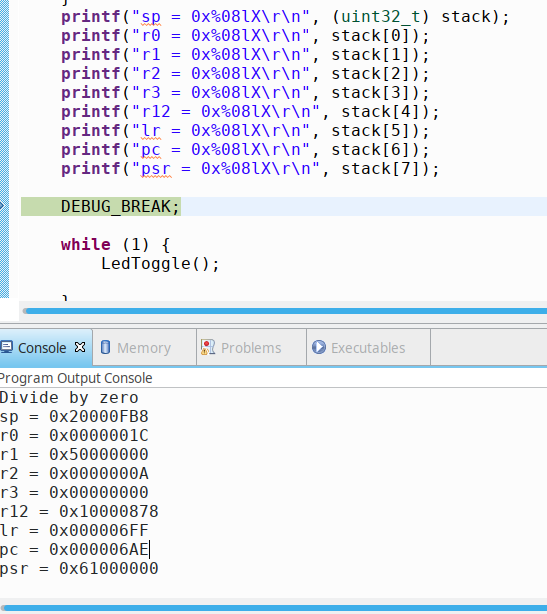
\includegraphics[width=0.65\textwidth, keepaspectratio]{imatges/HardFault_Console.png}}
 \caption{Debugger aturat a la instrucció DEBUG\_BREAK i el {\em dump} els registres}
 \label{fig:HardFaultDump}
\end{figure}


Per últim, es crida la macro {\bf DEBUG\_BREAK}\index{DEBUG{\_}BREAK}, que està definida com una instrucció en assemblador ({\bf BKPT \#01}) que posa el {\em core} en mode {\em Debug} i atura l'execució en aquest punt. Així, si tenim un {\em debugger} connectat, veurem com l'execució s'atura en aquest punt i torna el control a la nostra eina (veure Figura~\ref{fig:HardFaultDump}).


\begin{figure}
 \centering
 \fbox{\color{ocre}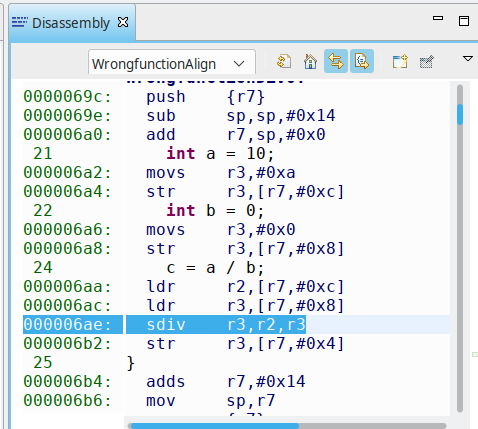
\includegraphics[width=0.65\textwidth, keepaspectratio]{imatges/HardFault_Dissassembly.png}}
 \caption{Codi assemblador a la posició de memòria indicada pel registre {\bf PC}}
 \label{fig:HardFaultDis}
\end{figure}

Si anem a la finestra {\em Disassembly} i anem a la posició de memòria que indica el registre {\bf PC} (0x6AE a l'exemple), veurem que apunta a una instrucció assemblador {\em sdiv}, que es corresponent amb una divisió. Si mirem el codi anterior, podem deduir que a la posició de memòria {\bf R7+0x8} (corresponent a la variable {\em b}) s'hi ha emmagatzemat un 0 (instruccions a 0x6A6 i 0x6A8) i aquesta variable es fa servir a la divisió com a divisor, causant l'error (veure Figura~\ref{fig:HardFaultDis}).

També cal comentar que les diferents funcions que generen errors són les següents:
\begin{itemize}
 \item {\bf WrongfunctionDiv0()}\index{WrongfunctionDiv0()} causa una divisió per zero.
 \item {\bf WrongfunctionAlign()}\index{WrongfunctionAlign()} causa un error d'accés a memòria fora d'alineament.
 \item {\bf WrongfunctionWrongMemory()}\index{WrongfunctionWrongMemory()} causa un error per accés fora dels límits de la memòria.
 \item {\bf fp()}\index{fp()} causa un intent d'executar a la posició 0x0000\_0000 de memòria.
\end{itemize}

\chapter{Baix cosum}
\label{ch:low-power}
Un dels temes més habituals de trobar-se quan es tracten temes amb microcontroladors és el del baix consum. Gràcies a la tecnologia de fabricació dels microxips i els avenços en les arquitectures dels microcontroladors, aquests han arribat a unes fites de consum molt baixes, permeten desenvolupar aplicacions on el sistema pugui anar alimentat per bateries o altres fonts d'alimentació alternatives a l'alimentació general. En aquest capítol veurem les característiques actuals dels microcontroladors en aquest aspecte, com treure tot el partit a aquestes característiques i, per últim, com adaptar els \gls{RTOS} per treballar amb baix consum.

Cal repassar uns quants conceptes sobre el consum d'energia abans d'introduir-nos de ple en el tema.

\section{Consideracions prèvies}
\label{sec:lowpowerintro}

Per la pròpia natura dels circuits digitals, aquests consumeixen sobretot quan el seu rellotge principal està actiu. Això fa que l'estratègia principal per reduir el consum d'un circuit és desactivar-li precisament el rellotge o reduir la seva freqüència, ja que el consum és proporcional a la velocitat de rellotge.
\begin{remark}
 Donat que el consum és quasi proporcional a la freqüència de rellotge, els fabricants acostumen a donar el consum per MHz (típicament $\mu$A/MHz).
\end{remark}

També cal tenir en compte que qui més consumeix en un microcontrolador és el propi {\em core} o CPU i que, per tant, serà el mòdul que caldrà tenir apagat el màxim de temps possible.

\section{Modes d'{\em sleep}}
\label{sec:sleepmodes}
Els diferents fabricants de microcontroladors basats en Cortex-M ofereixen diferents modes d'sleep, això és, diferents combinacions de perifèrics que estan actius a cada mode per tal de reduir el consum.

Així, els microcontroladors de Silicon Labs tenen 4 modes d'sleep\footnote{A més, hi ha el mode normal, on la CPU està a ple rendiment} \cite[6]{EFM32GRM}:
\begin{itemize}
 \item EM0 - {\em Energy Mode 0}: Tot el sistema està actiu incloent-hi tots els perifèrics.
 \item EM1 - {\em Energy Mode 1}: La CPU està desactiva i la resta de perifèrics estan disponibles.
 \item EM2 - {\em Energy Mode 2}: La CPU està desactivada i només els perifèrics de baix consum estan disponibles (UART, RTC, TIMER, Watchdog)
 \item EM3 - {\em Energy Mode 3}: Tot el sistema està desactivat, només es manté la RAM activada i certes interrupcions
 \item EM4 - {\em Energy Mode 4}: Tot el sistema està desactivat, només es pot fer un {\em reset} al sistema.
\end{itemize}

En canvi, els microcontroladors de ST tenen només 3 modes de baix consum\footnote{Versions de Cortex-M0+ tenen algun mode més} \cite[126]{STM32F4RM}:
\begin{itemize}
 \item {\em Run mode}: Tot el sistema està actiu incloent-hi tots els perifèrics.
 \item {\em Sleep mode}: La CPU està desactiva i la resta de perifèrics estan disponibles.
 \item {\em Stop mode}: Tot el sistema està desactivat, només es manté la RAM activada i certes interrupcions
 \item {\em Standby mode}: Tot el sistema està desactivat, només es pot fer un {\em reset} al sistema.
\end{itemize}

\begin{table}
\caption{Consum d'energia de diferents fabricants i modes (per un Cortex-M0+) \cite{EFM32ZG108DS}\cite{STM32L01}}
\centering
\begin{tabular}{|c|c|c|}
\hline
{\bf Processador} & {\bf STM32} & {\bf EFM32}\\
{\bf SleepMode} & & \\
\hline
{\bf EM0 - {\em Run mode}} &  76 $\mu$A/Mhz &  114 $\mu$A/MHz\\
\hline
{\bf EM1 - {\em Sleep mode}} & ~42  $\mu$A/MHz & 48 $\mu$A/MHz\\
\hline
{\bf EM4 - {\em Standby mode}} & 230 nA & 20 nA \\
\hline
\end{tabular}
\label{tb:bin_size}
\end{table}

Els {\em core} Cortex-M es poden posar en mode de baix consum fent servir dues instruccions {\bf WFI} i {\bf WFE}. El primer que cal fer és configurar a quin mode d'adormir es vol posar el microcontrolador i després executar la instrucció que pertoqui. La CPU es quedarà en l'estat de baix consum que s'hagi configurat fins que es generi una \gls{IRQ} per algun perifèric o generat per un senyal extern.

\section{Estratègies de baix consum}
\label{sec:lowpowerstrategies}
Vist tot l'anterior, l'estratègia bàsica per tenir un baix consum serà la de preparar els perifèrics per a que facin la funcionalitat d'entrada/sortida necessària de manera que llencin una \gls{IRQ} quan finalitzin, posar en un dels modes de baix consum on la CPU està desactivada a l'espera de les interrupcions; a continuació, la CPU processarà les dades o esdeveniments que hagin succeït i es tornarà a configurar els perifèrics i es tornarà a posar la CPU en mode baix consum, etc.

Per tant, quan es desenvolupa una aplicació per ser de baix consum, s'acostuma a treballar basant-se en interrupcions (Veure~\fullref{ch:IRQ}) i tenint la CPU el màxim de temps en algun dels modes de baix consum.

\subsection{Exemple de baix consum}
\href{https://github.com/mariusmm/cursembedded/tree/master/Simplicity/ADC_1_LP}{L'exemple que es veurà} farà servir l'\gls{ADC} per convertir una entrada analògica a un valor digital, com ja es a fer a l'exemple \fullref{sub:ADC_example}. En el cas de baix consum, es configura el perifèric de la mateixa forma però s'hi afegeix l'opció que generi una \gls{IRQ} quan acaba de fer una conversió. Així, el nostre codi al bucle principal engegarà la conversió, entrarà en el mode de baix consum {\bf EM1} perquè la CPU es quedi en repòs mentre l'ADC fa la seva feina i es desperti per la \gls{IRQ} de finalització; tot seguit es llegeix i es mostra la dada convertida.

\index{main()}\index{ADC{\_}Start()}\index{EMU{\_}EnterEM1()}\index{ADC{\_}DataSingleGet()}
\begin{lstlisting}[style=customc,caption={Bucle principal amb funcions de baix consum}, label=ADC_LP]
void main() {
  ...
  while (1) {
    ADC_Start(ADC0, adcStartSingle);

    EMU_EnterEM1();

    ADCvalue = ADC_DataSingleGet(ADC0);
    printf("ADC Value %lu\r\n", ADCvalue);
  }
  ...
}
\end{lstlisting}

Podem fer una mesura del temps que està la CPU en el mode EM1 posant un pin a '1' quan s'entra al mode i posar-lo a '0' quan se'n surt, tal com es veu al projecte d'exemple.

Si usem l'analitzador lògic per mesurar els temps, veiem la imatge de la Figura~\ref{fig:adc_logic} que les mesures diuen que 44,29 microsegons de 52.21 la CPU està en mode de baix consum (el 84.84\% del temps).

\begin{figure}
 \centering
 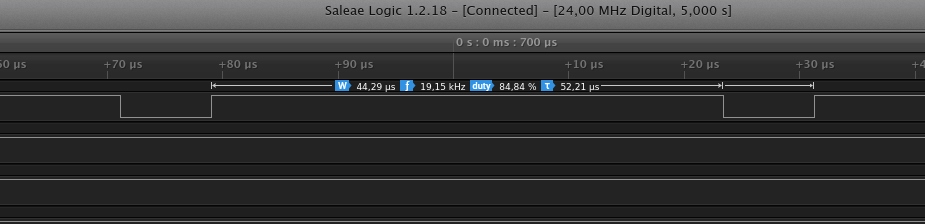
\includegraphics[width=0.85\textwidth, keepaspectratio]{imatges/ADC_LP1_Measurement.png}
 \caption{Captura de les mesures temps de l'analitzador lògic}
 \label{fig:adc_logic}
\end{figure}

\section{{\em Timers} de baix consum}
\label{sub:letimer_example}
Un mode que es fa servir sovint en sistemes de baix consum és el de tenir un {\em timer} configurat perquè desperti el sistema cada cert temps. Així per exemple, en un sistema que ha de llegir un sensor cada 30 segons, el {\em timer} seria l'únic perifèric en funcionament actiu i estaria configurat per generar una \gls{IRQ} cada 30 segons; la resta del microcontrolador podria estar en un mode de baix consum que el permeti consumir molt poca energia mentre espera a ser despertat per una \gls{IRQ}.

Al \href{https://github.com/mariusmm/cursembedded/tree/master/Simplicity/LETIMER_LP}{projecte del repositori} hi ha un exemple d'aquest tipus. Es fa servir un {\bf LETIMER}, que és un {\em timer} de baix consum i baixa freqüència que pot funcionar mentre la resta del microcontrolador està en el mode EM2 (o EM3 segons la configuració que es faci servir) \cite[294]{EFM32TGRM}. Aquest {\bf LETIMER} es pot alimentar amb el rellotge extern de baixa freqüència a 32.768 Hz ({\bf LFXO}) o bé amb l'oscil·lador intern a 1.000 Hz ({\bf ULFRCO}) (al codi es pot triar segons es defineixi o no la macro {\bf USE\_ULFRCO}). El rellotge que s'hagi triat es pre-escala per un factor suficient per tenir un comptador prou lent, ja que cal tenir en compte que aquest comptador és de només 16 bits i, per tant, si tenim una freqüència de funcionament elevada no podrem comptar gaire temps.
Tot seguit el {\em timer} es configura per generar una interrupció quan arribi a 0 (és un comptador decreixent) i el seu valor {\bf TOP} (al valor al que es reinicia després d'arribar a 0) es posa en funció de la freqüència de funcionament i el temps que es vol tenir el sistema en baix consum, a l'exemple del repositori es posa a 4 segons. Un resum del codi de l'exemple es veu a Llistat~\ref{LETIMER_example}.

\index{LETIMER0{\_}IRQHandler()}\index{main()}\index{LETIMER{\_}IntGet()}\index{LETIMER{\_}IntClear()}
\index{GPIO{\_}PinOutToggle()}\index{CMU{\_}ClockSelectSet()}\index{CMU{\_}ClockDivSet()}
\index{LETIMER{\_}CompareSet()}\index{EMU{\_}EnterEM3()}
\begin{lstlisting}[style=customc, caption={Exemple ús de {\bf LETIMER}}, label=LETIMER_example]
#define PRESCALER cmuClkDiv_1
#define EFECTIVE_CLK_FREQ (1000/PRESCALER)
#define SLEEP_SECONDS 4
#define TOP_VALUE (EFECTIVE_CLK_FREQ * SLEEP_SECONDS)

void LETIMER0_IRQHandler(void) {
	uint32_t flags;

	/* Clear flag for LETIMER0 */
	flags = LETIMER_IntGet(LETIMER0);
	LETIMER_IntClear(LETIMER0, flags);

	/* Toggle LED ON/OFF */
	GPIO_PinOutToggle(gpioPortD, 7);
}

void main(void) {
  ...
  /* ULFRCO is 1,000 kHz */
  CMU_ClockSelectSet(cmuClock_LFA, cmuSelect_ULFRCO);
  CMU_ClockDivSet(cmuClock_LETIMER0, PRESCALER);
  ...
  LETIMER_CompareSet(LETIMER0, 0, TOP_VALUE);
  ...
  while (1) {
    /* nothing to do here */
    EMU_EnterEM3(true);
  }
}
\end{lstlisting}

Aquest és un exemple senzill que fa servir un {\em timer} especial de la família EFM32 de Silicon Labs. Altres fabricants proporcionen {\em timers} similars. Així ST té un {\em timer} força similar, anomenat LPTIMER (\cite{ST_ANS4865}) i Fresscale te el LPTMR amb característiques similars \cite{Kinetis_LPTMR}. Els {\em timers} de ST i de Silicon Labs  poden generar senyals tipus \gls{PWM} mentre el microcontrolador està en modes de baix consum (veure \fullref{sub:PWM}).

\section{Baix consum i RTOS}
\label{sec:lowpwerRTOS}
Quan treballem amb un RTOS funcionant en el nostre microcontrolador, hi ha diferents estratègies per aconseguir disminuir el consum energètic.

Bàsicament hi ha dues estratègies:
\begin{itemize}
 \item Aprofitar la tasca {\em Idle} per posar al microcontrolador en un mode de baix consum.
 \item Passar a un sistema sense {\em tick} (també dit {\em tickless}).
\end{itemize}

En qualsevol cas, l'avantatge de que sigui el SO qui s'encarregui de gestionar el baix consum és que les tasques no s'han de preocupar per aquesta gestió.

\subsection{Tasca {\em Idle} per baix consum}
\label{sub:idlelowpower}
L'estratègia més senzilla és la d'activar un mode de baix consum quan s'executa la tasca {\em Idle}. Com que aquesta tasca s'executa quan no hi ha cap altra tasca preparada per agafar el microcontrolador, té sentit pensar en aturar el microcontrolador i esperar a que una tasca estigui disponible. Quan succeeixi el proper {\em tick}, el microcontrolador sortira del mode d'{\em sleep} i tornarà a executar el planificador, que, si segueix sense haver cap tasca disponible (en estat {\em Ready}) per executar tornarà a executar la tasca {\em Idle} que tornarà a adormir la CPU i es repetirà el cicle \cite{FreeRTOSLP}.

\begin{remark}
Cal recordar que quan el {\em core} està en algun mode de baix consum, el {\em SysTick} també es desactiva. Per tant, per poder tenir un {\em tick} quan el {\em core} està en un mode de baix consum caldrà fer servir un altre Timer que si que funcioni en aquests modes de baix consum.
\end{remark}

Cal pensar que tot i que aquest mètode és molt senzill d'implementar, té la limitació de que a cada {\em tick} es treu la CPU del mode de baix consum per comprovar si hi ha alguna tasca en estat {\em Ready}. Podem imaginar-nos una aplicació que llegeixi d'un sensor cada 200 ms i processant les dades, com l'aplicació d'exemple XXXXX. Si es té en compte que el {\em tick} pot ser de 1000 Hz, és fàcil d'observar que es despertarà molts cops al {\em core} perquè tant sols el planificador vegi que no hi ha cap tasca {\em Ready} i torni a adormir el processador.

%% manual break a la ultima macro pq latex no ho fa be
Aquesta característica es pot activar a FreeRTOS editant el fitxer ``FreeRTOSConfig.h'' i fixant a '0' la definició {\bf configUSE{\_}TICKLESS{\_}IDLE} i triant el valor '1' per {\bf configUSE\_SLEEP\_MODE\\\_IN\_IDLE}. En el cas de Silicon Labs, el microcontrolador es posa en el mode EM2 (veure \fullref{sec:sleepmodes}) i deixant en funcionament tant sols el RTC (veure \fullref{sub:RTC}) i les \gls{IRQ} dels GPIOs que l'usuari hagi configurat (veure \fullref{ch:IRQ}).

\subsection{FreeRTOS sense {\em tick}}
\label{sub:tickless}

L'altre estratègia per disminuir encara més el consum, és desactivar el {\em tick} durant cert temps. En una aplicació on totes les tasques estan bloquejades (i que entraria la tasca {\em Idle}) es pot calcular el temps en que alguna tasca es desbloquejarà (perquè alguna tasca estigui bloquejada perquè ha cridat la funció vTaskDelay()\index{vTaskDelay()}). Es pot desactivar el {\em Tick} i programar el Timer perquè generi una interrupció en aquell temps calculat. Si mentre està el sistema adormit esperant aquell temps hi ha algun esdeveniment extern (interrupció), es despertarà i es podrà reprendre l'execució normal i tornar a activar el {\em Tick}.

Amb aquesta estratègia es maximitza el temps en que el {\em core} està en algun dels modes de baix consum i per tant es pot reduir dràsticament el consum d'una aplicació (veure \fullref{ch:low-power}).

En el cas de FreeRTOS, el port disponible per Cortex-M ja incorpora aquesta característica, i es pot configurar editant el fitxer ``FreeRTOSConfig.h'', concretament fixant el valor '1' a la macro {\bf configUSE\_TICKLESS\_IDLE}. En el cas de Silicon Labs, el microcontrolador es posa en el mode EM2 igual que en cas amb {\em ticks} i es programa el RTC perquè generi una \gls{IRQ} en el temps adequat.

En ambdós casos el codi que gestiona el baix consum i els {\em ticks} en el port FreeRTOS està al fitxer {\bf low\_power\_tick\_management.c} a la funció {\bf vPortSetupTimerInterrupt()}\index{vPortSetupTimerInterrupt()}.

\chapter{Documentant el codi}
\label{sec:documentant}
Un tema recurrent en temes d'enginyeria del software és com documentar el codi font que es desenvolupa per tal d'afavorir, sobretot, el manteniment del codi durant el temps i algú altre (o nosaltres mateixos) haguem de modificar, re-uilitzar o arreglar algun problema. No farem aquí una discussió sobre els beneficis de documentar, quan fer-ho, etc.

Hi diferents tècniques i mètodes de documentar el codi, aquí veurem només una, basada en Doxygen. Aquest programa processa la documentació inserida dins el propi codi font i genera diferents sortides, la més habitual és una carpeta html amb tota la documentació ben bonica i accessible amb un navegador (té altres formats de sortida, com .pdf, .doc, etc.). Per documentar el nostre codi, el que cal que fem és escriure la documentació dins el propi codi com a comentaris de codi seguint unes normes i {\em tags} molt senzills propis de Doxygen. (veure Figura~\ref{fig:doxygencode}). Aquest mètode de documentar ha esdevingut un estàndard de facto i es troba arreu. Per documentar-se sobre com treballar amb Doxygen, la seva pàgina web està força bé amb exemples de tots tipus \cite{Doxygen}.

\begin{figure}
 \centering
 \fbox{\color{ocre}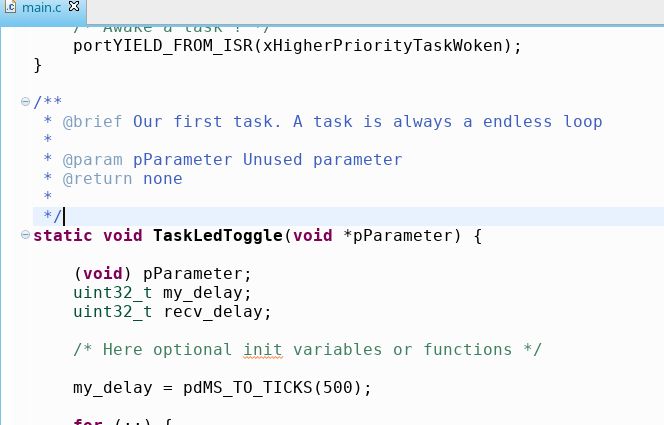
\includegraphics[width=0.85\textwidth, keepaspectratio]{imatges/Doxgen3.png}}
 \caption{Comentari per doxygen dins un codi}
 \label{fig:doxygencode}
\end{figure}

A simplicity (i de fet, a qualsevol IDE basat en Eclipse), podem activar Doxygen com l'eina de documentació, i d'aquesta manera l'editor ens ajudarà alhora d'escriure-la, ja que, per exemple, en escriure «/**» davant una funció ens inserirà automàticament el codi Doxygen per documentar-la (incloent-hi tots els paràmetres), simplificant molt la nostra feina.

Una bona opcio és afegir un directori on ficar-hi el fitxer de configuració del Doxygen (directori /Doc) i on es genera el codi html (directori /Doc/html). El Doxygen s'executa dins del directori /Doc i es genera el codi html (o pdf, o rtf, o el que calgui). Si al fitxer Doxygen li posem l'extensió .doxyfile el propi simplicity el reconeix com a fitxer de documentació i podem executar Doxygen pitjant el botó amb una arroba de color blau a la barra d'eines (Figura~\ref{fig:doxygenbutton}).

\begin{figure}[h!]
 \centering
 \fbox{\color{ocre}
\includegraphics[width=0.35\textwidth, keepaspectratio]{imatges/Doxygen_button.png}}
 \caption{Botons de Simplicity, l'arroba blava permet executar Doxygen}
 \label{fig:doxygenbutton}
\end{figure}


També podrem editar de forma visual el fitxer de configuració fent-hi doble-click i veure el resultat obrint dins del Simplicity el fitxer /Doc/html/index.html (Figura~\ref{fig:doxygenconfig}).

\begin{figure}
 \centering
 \fbox{\color{ocre}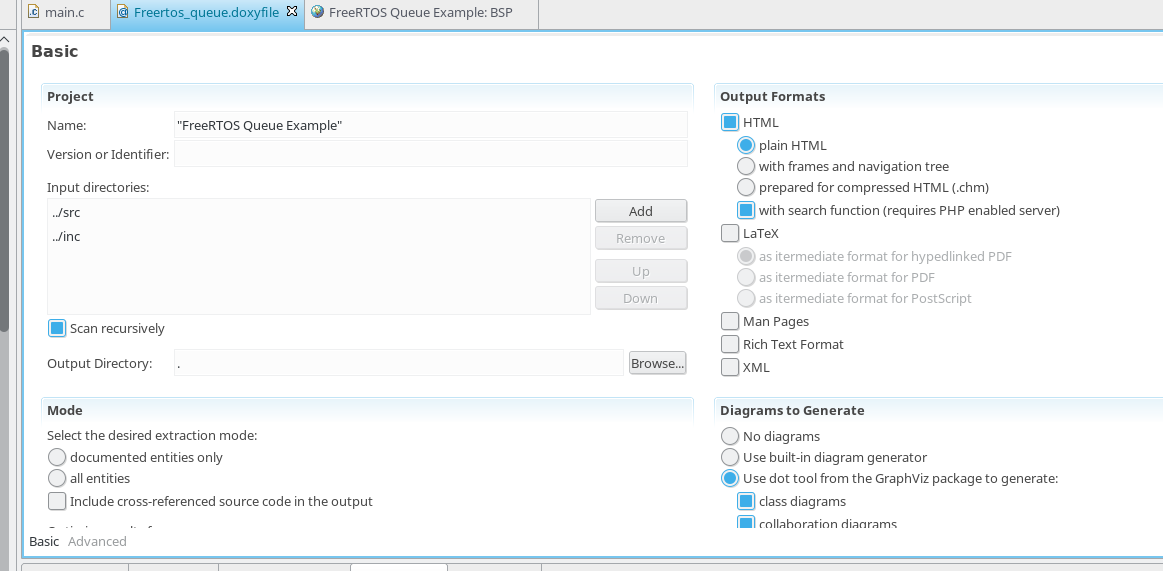
\includegraphics[width=0.85\textwidth, keepaspectratio]{imatges/Doxygent_configuration.png}}
 \caption{Configuració de Doxygen dins de Simplicity}
 \label{fig:doxygenconfig}
\end{figure}

Hi ha un exemple complet al projecte FreeRTOS Queue (veure \fullref{sub:cues_exemple}). En aquest cas, l'explicació del projecte (la secció principal anomenada mainpage en Doxygen) està al final del fitxer main.c. També hi ha la possibilitat de posar aquesta secció en un fitxer a part, normalment un fitxer README.md. Si ho fem així, aquest fitxer README.md github el presenta a la pàgina principal del projecte. El fitxer generat també es pot obrir dins el propi Simplicity Studio (Figura~\ref{fig:doxygeneclipse}).

A més, si configurem com cal github, podem pujar el codi html generat per Doxygen al repositori i veure'l a un adreça de github. La de l'exemple està a \href{https://mariusmm.github.io/cursembedded/Simplicity/FreeRTOS_1/Doc/html/}{aquí} \cite{GITHUBPages} i es pot obrir des d'un navegador qualsevol,

\begin{figure}
 \centering
 \fbox{\color{ocre}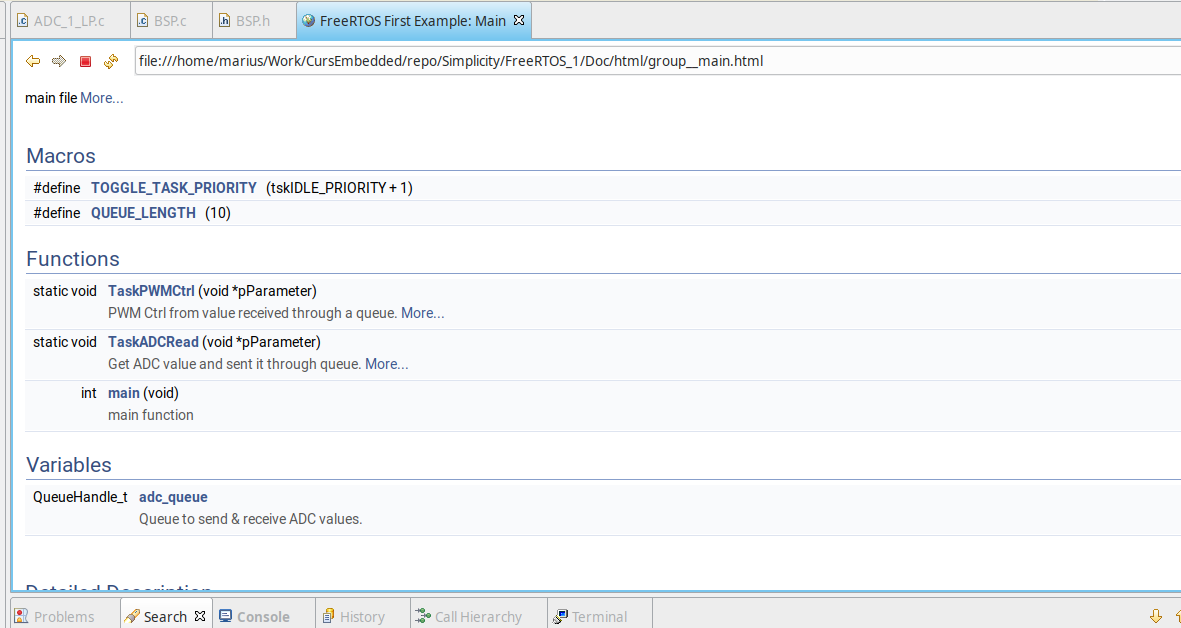
\includegraphics[width=0.85\textwidth, keepaspectratio]{imatges/DoxygenEclipse.png}}
 \caption{Pàgina web de documentació vista dins de Simplicity Studio, en aquest cas es visualitza un dels fitxers locals}
 \label{fig:doxygeneclipse}
\end{figure}

\chapter{Bones pràctiques}

En aquest capítol veurem una sèrie de bones pràctiques habituals en la programació de sistemes encastats. Aquestes bones pràctiques donen consells i guia sobre com dissenyar o programar parts de codi per evitar problemes que, habitualment, són molt complicats de detectar.
%% Veure Michael Barr Bugs1-5.pdf i Bugs6-10.pdf

\section{Ús de memòria dinàmica}
Una de les diferències més notables a l'hora d'escriure codi per un sistema encastat és l'ús de memòria dinàmica. Bàsicament se'n desaconsella totalment el seu ús en sistemes encastats. Això es deu al fet que tenim molt poca memòria RAM disponible (pocs KB) i que la possible fragmentació que s'origina en fer-ne un ús dinàmic poc exhaurir-la molt més fàcilment. A més, el fet d'usar memòria dinàmica fa que el sistema sigui menys predictible, ja que en certs casos, l'ordre en que s'executen diferents {\em malloc()} pot ser diferent a cada execució.

És per això que no s'acostuma a usar memòria dinàmica en sistemes encastats. Si, tot i la recomanació de no fer-ho, és necessari alguna mena de gestió dinàmica de la memòria, la millor opció és proveir-se d'una estructura pròpia {anomenada \em pool} de blocs d'una mida predeterminada que proporcionin aquesta funcionalitat. D'aquesta manera s'evita la fragmentació ja que tots els blocs tenen la mateixa mida.

\section{Ús de {\em volatile}}
Com ja s'ha comentat a \fullref{sb:volatile}, errors en l'ús de la paraula reservada {\em volatile} poden ocasionar {\em bugs} difícils de trobar al nostre codi. Per tant, i com a recordatori, cal definir una variable com a {\em volatile} en el següents casos:
\begin{itemize}
 \item Variable global que comunica una ISR amb una funció.
 \item Variable comptador d'un bucle per implementar un {\em delay}.
 \item Punter a una adreça de memòria corresponent a un perifèric mapat a memòria.
 \item Variable global que hi accedeixen dues o més tasques d'un RTOS.
\end{itemize}

Cal recordar que l'ús de {\em volatile} farà que les optimitzacions del compilador no s'apliquin a la variable definida com a tal.

\section{Funcions re-entrants}
Com ja es va comentar breument a \fullref{sec:wrapperI2C}, quan es treballa en un entorn multitasca (com quan es té un RTOS) cal tenir en compte que funcions que puguin ser utilitzades alhora per més d'una tasca cal que siguin re-entrants. També cal adonar-se que una biblioteca per un perifèric HW qualsevol segurament haurà de ser re-entrant, ja que diverses crides simultànies sobre el mateix HW pot ocasionar errors de funcionament.

La norma general és de protegir cada funció que hagi de ser re-entrant amb un {\em Mutex}. La funció en qüestió intentarà agafar el {\em Mutex} a l'inici de la seva execució i el retornarà en quan acabi. En el cas de biblioteques per accedir a HW, és habitual tenir un sol {\em Mutex} compartit per tota la biblioteca i que es crea quan es crida a la funció d'inicialització de la biblioteca (veure \fullref{sec:wrapperI2C}).

\section{\em Deadlock}
Un {\em Deadlock} és una situació on diverses tasques tenen una dependència circular entre elles i queden totes elles bloquejades esperant-se unes a les altres.

Per evitar aquestes situacions, sovint complexes de detectar, hi ha dues recomanacions:
\begin{itemize}
 \item Evitar adquirir dos o més {\em Mutex}. Provar d'agafar dos o més {\em Mutex} pot provocar que s'agafi un però fallin els demès, fent que la tasca hagi d'esperar a d'altres tasques els alliberin, que potser necessiten del primer {\em Mutex}.
 \item Ordenar els {\em Mutex} de manera que, si s'ha d'agafar més d'un, totes les tasques segueixin el mateix ordre.
\end{itemize}

Amb aquests dues recomanacions es poden evitar la majoria de {\em deadlocks} generats per l'ús de {\em mutex} entre tasques.

\section{Inversió de prioritats}
\label{sec:priorityinv}
Quan tenim un parell de tasques que comparteixen un recurs, una amb poca prioritat ($T_l$) i la segona amb més prioritat ($T_h$), si s'afegeix una tercera tasca amb una prioritat intermèdia ($T_m$) al sistema, podem tenir un problema d'inversió de prioritats. Això passarà quan la tasca de menys prioritat agafa el recurs compartit amb ($T_h$). En aquest moment, si la tasca de prioritat intermèdia està a l'estat {\em Ready}, passarà a executar-se, fent que la tasca ($T_l$) no s'executi i retardant l'execució de la tasca ($T_h$), fent que, de fet, la prioritat de $T_h$ i $T_m$ s'hagin invertit, ja que la tasca amb prioritat intermèdia es pot executar tot el temps que vulgui i la tasca més prioritària no té la oportunitat \cite[101]{RTEmbeddedSystems}.

La manera més senzilla de resoldre aquest problema és usar {\em Mutex} amb herència de prioritats. Aquest mecanisme fa que, provisionalment, la tasca que agafa el {\em Mutex} pugi temporalment la seva prioritat a la mateixa de la tasca que l'està esperant \cite[106]{RTEmbeddedSystems}. FreeRTOS suporta aquest mecanisme als seus {\em Mutex}, i per tant fent un bon ús dels mateixos evitarem aquest fenomen d'inversió \cite[251]{FreeRTOSBook}.

\section{Assignació de prioritats}
\label{sec:priorities_RMA}
Sovint un dels dubtes que sorgeixen en el disseny de sistemes encastats és quines prioritats cal donar a cada una de les tasques del sistema. Existeix un algorisme molt senzill per assignar les prioritats a cada tasca, basant-se en el temps de procés que necessita cada una. Aquest algorisme s'anomena {\em Rate-Monotonic Algorithm} (RMA) i fa les següents assumpcions \cite{RMA_1}\cite[136]{EmbeddedBook_2}:
\begin{itemize}
 \item Totes les tasques són periòdiques.
 \item El {\em deadline} de cada tasca és el seu període.
 \item Totes les tasques són independents.
 \item Totes les tasques són pre-emtives i el cost d'aquest és negligible.
\end{itemize}

Aquest algorisme senzillament assigna la prioritat més alta a les tasques amb un període més curt. Així, s'ordenen les tasques segons el seu període (primer els períodes més curts) i s'assignen les prioritats, de més alta a més baixa.

Per saber si es podran executar totes les tasques dins dels seus límits complint tots els {\em deadline} es poden fer els següents càlculs:

Sigui $c_i$ el temps d'execució de la tasca $T_i$. Sigui $p_i$ el període d'execució de la tasca $T_i$. Sigui $n$ el nombre de tasques totals.
Es defineix l'ús acumulat $\mu$ a:
\begin{equation*}
 \mu = \sum^{n}_{i=1}\frac{c_i}{p_i}
\end{equation*}

S'ha de complir la condició \ref{eq:RMA} perquè es compleixin tots els {\em deadlines} de totes les tasques.
\begin{equation}
\label{eq:RMA}
 \mu \leq n (2^{1/n}-1)
\end{equation}

\begin{table}[b]
\caption{Dades d'exemple de tasques i prioritats (temps en mil·lisegons)}
\label{tb:RMA_example}
\centering
\begin{tabular}{|c|c|c|}
\hline
{\bf Tasca} & {\bf Període $p$} & {\bf Temps d'execució $c$}\\
\hline
T1 & 500 & 20\\
\hline
T2 & 250 & 30\\
\hline
T3 & 100 & 15\\
\hline
\end{tabular}
\end{table}

Així, si tenim 3 tasques amb les dades d'execució de la Taula~\ref{tb:RMA_example} l'algorisme RMA assignarien les prioritats de la següent manera:

\begin{enumerate}
 \item T3 més prioritària.
 \item T2 prioritat intermèdia.
 \item T1 baixa prioritat.
\end{enumerate}

També es pot calcular $\mu$
\begin{equation*}
 \mu = \frac{20}{500} + \frac{30}{250} + \frac{15}{100} = 0.31
\end{equation*}
i segons l'Equació~\ref{eq:RMA} tindrem que
\begin{equation*}
 0.31 \leq n (2^{1/n}-1) = 3(2^{1/3}-1) \approx 0.78
\end{equation*}

Per tant es compleixen les condicions perquè les tres tasques es puguin executar sense perdre cap esdeveniment. L'algorisme RMA dona una conjunt de prioritats que és òptima, per tant, si no es compleixen els {\em deadlines}, cap altre mètode d'assignar prioritats fixes podrà aconseguir-ho. En aquest cas caldrà tenir un {\em scheduler} amb un algorisme de prioritats dinàmiques.

També val la pena observar que la part dreta de l'Equació~\ref{eq:RMA} té un límit:
\begin{equation*}
 \lim_{n\to\infty} n \cdot (2^{1/n}-1) = ln(2) \approx 0.7
\end{equation*}

que ens indica que amb les condicions dites abans, un sistema amb moltes tasques no podrà tenir la CPU al 100\%, si no tant sols al 70\% d'ocupació total.

\section{Mida de les cues}
\label{sec:mida_cues}
Quan hem parlat de les cues en un \gls{RTOS} a \fullref{sec:queue}, hem dit que a l'hora de la seva creació cal especificar el tipus de dades que emmagatzemarà cada element de la mateixa i el nombre d'elements d'aquest tipus que la cua manegarà.

Però, com saber quants elements cal atorgar a una cua en la seva creació. Aquest paràmetre serà clau, ja que si creem una cua amb pocs elements disponibles, la tasca productora potser es quedi bloquejada si la tasca consumidora no va prou de pressa. Tot i que es pot triar aquest valor d'una forma empírica, començant per un valor prou baix i fent proves i via successives aproximacions arribar a un valor prou bo.

Aquest mètode, però, no ens assegura que en qualsevol cas el sistema no acabi amb una cua plena. Per això, cal un anàlisi més analític del problema per trobar una solució.

\subsection{Model M/M/1}
\label{sub:mm1}

Aquest model de cues és dels models estadístics més senzills però que ens pot donar informació important només amb les dades més bàsiques del nostre sistema. Aquest model fa certes suposicions que podem donar per bones pels nostres sistemes \cite{mm1_1}\cite{mm1_2}\cite{mm1_3}\cite{mm1_4}:
\begin{itemize}
 \item El productor genera noves entrades a la cua seguint una distribució de Poisson.
 \item El consumidor processa dades a la cua seguint una distribució exponencial.
 \item Només hi ha un productor.
 \item La cua és de tipus FIFO.
\end{itemize}

Amb aquestes suposicions ens cal trobar els paràmetres $\lambda$ i $\mu$ pel productor i el consumidor respectivament.

Si la nostra tasca consumidora genera un element nou a la cua cada certs $Pr$ temps tindrem:
\begin{equation}
 Pr = \text {temps mitjà a generar una dada}
\end{equation}
i llavors tindrem que
\begin{equation}
 \lambda = \frac{1}{Pr}
\end{equation}

El mateix càlcul el podem fer pel temps de la tasca consumidora:
\begin{equation}
C = \text {temps mitjà a processar una dada}
\end{equation}
i llavors tindrem que
\begin{equation}
 \mu = \frac{1}{C}
\end{equation}

Amb aquestes dades, tenim les següents fórmules:

\begin{equation}
 p = \frac{C}{Pr} = \frac{\lambda}{\mu}
\end{equation}

Aquesta primer valor $p$ ens indica si el sistema és factible o no: si $p$ és més petit d'1 ($p < 1$), la cua té sentit, en cas contrari, el ritme de inserir elements a la cua és més ràpid que el ritme de treure'ls i, per tant. la cua acabarà col·lapsant en algun moment o altre.

Amb aquest valor $p$ (o amb $Pr$ i $C$) podem obtenir els següents càlculs:

Nombre mitjà d'elements a la cua
\begin{equation}
 L_q = \frac{p^2}{(1-p)}  = (\frac{C}{Pr})^2 / (1 - \frac{C}{Pr})
\end{equation}
Temps mitjà de vida a la cua
\begin{equation}
 W_q =  \frac{p}{\mu - \lambda} = \frac{L_q}{\lambda} = L_q \cdot Pr
\end{equation}
Temps total d'una dada
\begin{equation}
 W = W_q + \frac{1}{\mu} = W_q +C = \frac{C}{1-p}
\end{equation}
Nombre mitjà d'elements al sistema
\begin{equation}
 L = \frac{p}{(1-p)}  = W \cdot \lambda = \frac{W}{Pr}
\end{equation}
Probabilitat que la cua tingui més de K elements
\begin{equation}
\label{eq:Prob_queue_full}
 P(\geqslant K) = p^K =  (\frac{C}{Pr})^k
\end{equation}

Així si, per exemple, tenim una tasca productora que genera una dada cada 50 ms i una tasca consumidora que processa les dades en uns 30 ms de mitjana, tenim els següents resultats:
\begin{equation*}
Pr = 50 \text{ ms}
\end{equation*}
\begin{equation*}
C = 30 \text{ ms}
\end{equation*}
\begin{equation*}
p = \frac{C}{Pr} = \frac{30}{50} = 0.6
\end{equation*}
\begin{equation*}
\text{Nombre mitjà d'elements a la cua } L_q = (\frac{30}{50})^2 / (1 - \frac{30}{50})  = 0.9
\end{equation*}
\begin{equation*}
\text{Temps mitjà de vida a la cua } W_q = 0.9 \cdot 50 = 45 \text{ ms}
\end{equation*}
\begin{equation*}
\text{Temps total de vida d'una dada } W =  \frac{30  \cdot 50}{50-30} = 75 \text{ ms}
\end{equation*}
\begin{equation*}
\text{Nombre mitjà d'elements al sistema } L =  \frac{75}{50} = 1.5
\end{equation*}
\begin{equation*}
\text{Probabilitat que la cua tingui més de 10 elements } P(\geqslant 10) =  (\frac{30}{50})^{10} \approx 0,00605 \rightarrow 0.60 \%
\end{equation*}

Aquestes equacions ens indiquen que durant bona part del temps de funcionament del sistema, la cua entre els dos processos tindrà tant sols 1 element, i que la probabilitat que tingui més de 10 elements en algun moment és de només el 0,60\%.
Cal fer notar que aquest valor probabilístic té en compte que els processos es comporten com una variable aleatòria tipus Poisson i tipus exponencial. Si algun dels dos processos no es comporta com a tal, si no que el seu temps de procés o de generació de dades és fix, els valors $L_q$, $W_q$, $W$ i $L$ seran certs en tot moment.

Manipulant una mica les fórmules, també podem esbrinar quin temps màxim de procés podem tenir per una tasca que genera dades cada 25 ms i volem menys d'un 0.1\% de probabilitats que s'ompli una cua de 8 elements.

Tenim, doncs:
\begin{equation*}
 Pr = 25 \text{ ms}
\end{equation*}
\begin{equation*}
 K = 8
\end{equation*}
Segons la fórmula \ref{eq:Prob_queue_full}:
\begin{equation*}
 \text{Probabilitat que la cua tingui més de K elements} = p^K =  (\frac{C}{Pr})^K < 0.001 (0.1\%)
\end{equation*}

per tant tenim que
\begin{equation*}
C^8 < 25^8*0,001  \rightarrow C < \sqrt[8]{25^8 * 0,001} \approx 10.54 \text{ ms}
\end{equation*}

Això ens indica que el temps de processar una dada per part el consumidor ($C$) ha de ser menor de 10.54 mil·lisegons de mitjana per assegurar els requeriments donats.


% \section{\em Debounce}
% %% SwitchDebouncing.pdf - SwitchDebouncingMore.pdf

\section{Ús eficient de printf}

Com ja es va veure a \fullref{sub:console_example} és possible tenir la funció {\bf printf()}\index{printf()} en els nostres sistemes encastats, pagant el preu de gastar força memòria \gls{FLASH} per la seva implementació.

Una opció recomanable en cas que l'ocupació de la memòria FLASH pugui ser un problema, és el de tenir diferents versions de {\bf printf()} segons els paràmetres que pot rebre. Així, enlloc de tenir el {\bf printf()} genèric de la biblioteca que accepta tot de tipus de tipus de dades segons el format tindrem una funció per imprimir un enter en decimal, una altra per imprimir un enter en hexadecimal, una funció per imprimir una cadena, etc. com es pot veure al Llistat~\ref{printf_variable}

A més, totes aquestes noves funciones les usarem a través d'una \gls{macro} de C, de forma que quan passem a una compilació de {\em release} del projecte aquests {\bf printf()} desapareguin del nostre codi. 

\index{printf{\_}char()}\index{printf{\_}string()}\index{printf{\_}hex8()}\index{printf{\_}int()}
\begin{lstlisting}[style=customc,caption={Diferents implementacions de {\bf printf()}},label=printf_variable]

void printf_char(char ch) {
  ITM_SendChar(ch);
}

void printf_string(char* str) {
  int i = 0;
  while(str[i]) {
    printf_char(str[i]);
    i++;
  }
}

void printf_hex8(uint8_t val) {
  if ((val >>4) > 9) {
    printf_char((val>>4) + '0' + 7);
  } else {
    printf_char((val>>4) + '0');
  }
  if ((val&0x0F) > 9) {
    printf_char((val&0x0F) +'0' + 7);
  } else {
    printf_char((val&0x0F) +'0');
  }
}

...

void printf_int(int val) {
  int rem_dec;
  int dec;
  int i;
  char buffer[10];
    
  i = 0;
    
  if (val < 0) {
    printf_char('-');
    val = -1 * val;
  }

  dec = val;
  rem_dec = val;

  do {
    rem_dec = dec%10; 
    dec /= 10; 
    buffer[i] = '0'+rem_dec;
    i++;
  } while(dec > 10);
  buffer[i] = '0' + dec;

  /* print reverse buffer */
  for(; i >= 0; i--) {
    printf_char(buffer[i]);
  }
}
\end{lstlisting}

\chapter{Empaquetant estructures}
\label{ch:estructures}

L'ús d'estructures ({\em struct} en C) per emmagatzemar dades que estan relacionades és força habitual. Per fer-ho, només cal definir una estructura i cada camp es defineix amb el tipus desitjat. Tota l'estructura funciona com un paquet de dades, que es pot moure, copiar i accedir com un tot.

Però si volem accedir a baix nivell a aquestes estructures per, per exemple, enviar les dades que conté per un port sèrie, inserir-la a un paquet de xarxa o enviar-ho a un altre dispositiu via SPI o I2C, cal que tinguem compte el problema de l'empaquetament.

Quan definim una estructura en C, el compilador ha de decidir com l'emmagatzema a la memòria. Segons les característiques dels busos i l'arquitectura del microcontrolador, pot ser que els accessos a memòria només es puguin fer a nivell de paraula (en el cas d'ARM una paraula és de 32 bits) i que no es pugui accedir a un byte individual de la memòria.

I com afecta això a les estructures? Doncs que el compilador pot optar a col·locar els diferents camps de l'estructura ocupant cada un una posició de memòria enlloc d'empaquetar-los tant com pugui.

Així, si tenim una estructura definida com es veu al Llistat~\ref{unpacket_struct} el compilador guardarà l'estructura a la memòria tal com es veu a la Figura~\ref{fig:UnpackedMemoryStructure}. 

\begin{lstlisting}[style=customc,caption={Estructura d'exemple},label=unpacket_struct]
 struct {
	uint8_t fieldS1;
	uint16_t fieldS1b;
	uint32_t fieldL1;
	uint32_t fieldL2;
	uint8_t fieldS2;
} unpacket_struct;
\end{lstlisting}


\begin{figure}
 \centering
 \fbox{\color{ocre}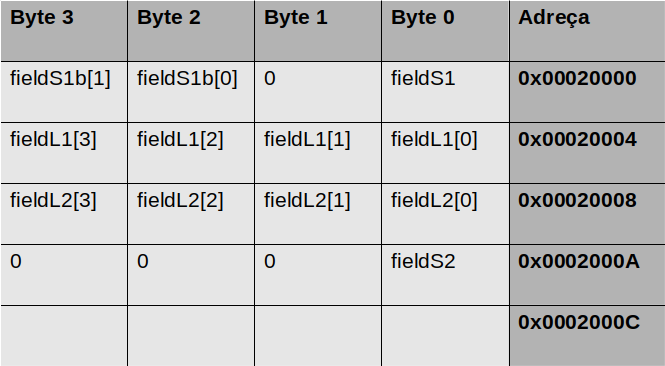
\includegraphics[width=0.85\textwidth, keepaspectratio]{imatges/Estructures.png}}
 \caption{Disposició de l'estructura a la memòria}
 \label{fig:UnpackedMemoryStructure}
\end{figure}

Que com es pot veure aquesta organització no és la que ens podríem esperar, ja que el camp {\bf fieldS1b} no està enganxat al camp {\bf fieldS1} i es per una posició de memòria per allà enmig. Aquesta operació s'anomena {\em padding} i és força habitual en totes les arquitectures. En aquest cas fa que aquesta estructura ocupi 16 bytes a la memòria enlloc dels 12 que podria ocupar si estigues tot ben empaquetat.

Això no s'acostuma a tenir gaire en compte alhora de programar sistemes encastats, però pot ser força important si en algun moment una estructura d'aquest estil cal enviar-la byte a byte a algun mòdul o perifèric. Anem a suposar que enviarem aquesta estructura d'exemple pel port sèrie. Si fem una funció que vagi llegint byte a byte l'estructura, tindrem que llegirà uns buits a 0 enmig que ens esgarraran el resultat.

En aquests casos, cal dir-li al compilador que volem que empaqueti tant com pugui l'estructura. Això és fa amb una comanda pròpia de cada compilador, en el cas de GCC és la comanda {\bf \_\_attribute\_\_} que es fa servir tal com es veu al Llistat~\ref{packet_struct}. Amb aquesta comanda l'estructura a memòria queda com es veu  a la Figura~\ref{fig:UnpackedMemoryStructure}.


\begin{lstlisting}[style=customc,caption={Estructura d'exemple empaquetada},label=packet_struct]
struct __attribute__ ((__packed__)) {
	uint8_t fieldS1;
	uint16_t fieldS1b;
	uint32_t fieldL1;
	uint32_t fieldL2;
	uint8_t fieldS2;
} packet_struct;
\end{lstlisting}


\begin{figure}
 \centering
 \fbox{\color{ocre}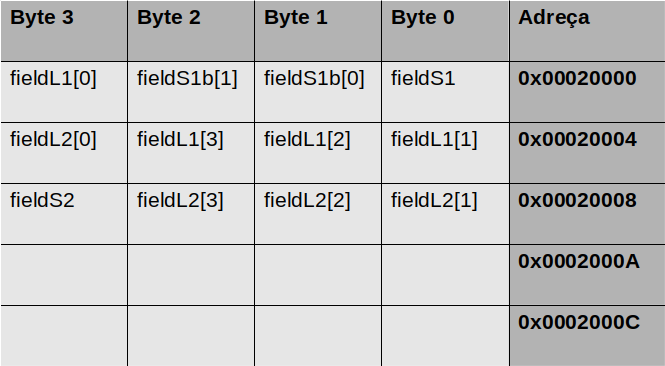
\includegraphics[width=0.85\textwidth, keepaspectratio]{imatges/Estructures2.png}}
 \caption{Disposició de l'estructura empaquetada a la memòria}
 \label{fig:UnpackedMemoryStructure}
\end{figure}

Fent servir aquest atribut es veu que està tot ben empaquetat i ens estalvia uns quants bytes. A més, s'han omplert tots els forats de manera que ara si que podrem accedir byte a byte l'estructura sense problemes.

Cal dir que en força casos aquestes estructures empaquetades poden ser més lentes d'accedir-hi, ja que la CPU haurà d'accedir a diferents posicions de memòria i reconstruir el valor original movent bits amunt i avall (veure per exemple, com es reconstruiran els camps fieldL1 o fieldL2)

\section{Un exemple senzill}

A l'\href{https://github.com/mariusmm/cursembedded/tree/master/Simplicity/Structures}{exemple del repositori} es defineixen dos estructures iguals, una amb l'atribut per empaquetar-la i l'altra amb les opcions per defecte.

Primer es treuen per la consola les mides de totes dues estructures, que encaixen amb el que hem dit aquí i tot seguit es pinten byte a byte per observar els zeros enmig i com està emmagatzemada cada estructura.

Cal destacar com s'accedeix byte a byte a l'estructura. Es defineix un apuntador a byte ({\em uint8\_t} *) i es fa apuntar a l'adreça d'inici de l'estructura que es vol analitzar. Tot seguit es va imprimint byte a byte el contingut de la memòria on està emmagatzemada l'estructura.

\begin{lstlisting}[style=customc,caption={Estructura d'exemple empaquetada},label=struct_example]
...
  uint8_t *buffer;

  buffer = (uint8_t*) &unpacket_struct;
  printf("Unpacket structure: \t");
  for(i = 0; i < sizeof(unpacket_struct); i++) {
	  printf("0x%02X, ", buffer[i]);
  }
  printf("\n");
...
\end{lstlisting}


També es pot analitzar directament el contingut de la memòria usant l'IDE Simplicity Studio fent servir l'eina de {\em dump} de la memòria tal com es veu a la Figura~\ref{fig:UnpackedMemoryStructure}.

\begin{figure}
 \centering
 \fbox{\color{ocre}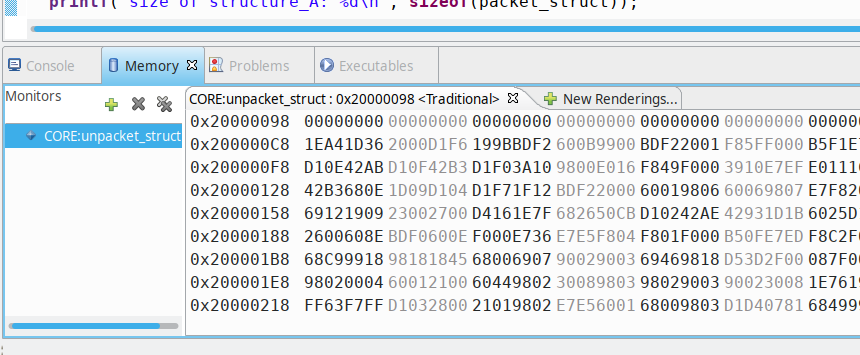
\includegraphics[width=0.85\textwidth, keepaspectratio]{imatges/MemoryDumpStructure.png}}
 \caption{Detall de la finestra de {\em memory dump} a Simplicity Studio}
 \label{fig:UnpackedMemoryStructure}
\end{figure}


\chapter{CMSIS}
\label{ch:CMSIS}
\gls{CMSIS} és una proposta d'ARM per unificar les diferents biblioteques dels fabricants sota una sola especificació, de manera que un disseny es pugui migrar a un altre fabricant de Cortex sense gaires problemes. Hi ha diferents subconjunts d'aquesta proposta, anem a veure'ls un a un.

\section{CMSIS-Core}
\label{sec:CMSIS-Core}
Aquesta part de l'especificació fixa la forma de comunicar-se amb les parts més {\em core} de la CPU, com son: el mapa de memòria (\fullref{sub:memory-mapped}), el sistema d'excepcions (\fullref{ch:exceptions}), els registres de control de la CPU, el gestor d'interrupcions (\fullref{ch:IRQ}), el Systick (\fullref{sec:systick}) i les {\em caches} \cite{CMSIS-CORE}. En aquesta biblioteca s'inclouen també els fitxers d'inicialització de cada microcontrolador en concret (\fullref{sub:boot}).

Així, i a tall d'exemple, les funcions que ja hem fet servir per controlar interrupcions com {\bf NVIC\_EnableIRQ()}\index{NVIC{\_}EnableIRQ()} a \fullref{ch:IRQ} no són pròpies de cap fabricant si no que són funcions definides per {\bf CMSIS-core}. També la manera en que es defineixen estructures per accedir als diferents perifèrics ve marcada per l'especificació {\bf CMSIS-Core} (veieu \fullref{devinfo}).

\section{CMSIS-Driver}
% \cite{CMSIS-DRIVER}
Aquesta especificació defineix una \gls{API} per tot un seguit de perifèrics per tal que els fabricants puguin implementar el {\em driver} corresoonent i els desenvolupadors no hagin de dependre de llibreries pròpies de cada fabricant. Aquesta especificació inclou els següents perifèrics:
\begin{itemize}
 \item \gls{CAN}
 \item Ethernet
 \item I2C
 \item \gls{MCI}
 \item  NAND 
 \item Flash
 \item \gls{SAI}
 \item SPI
 \item Storage
 \item USART
 \item USB
\end{itemize}


\section{CMSIS-DSP}
\label{sec:CMSIS-DSP}
Aquesta biblioteca inclou totes les funcions específiques de tipus \gls{DSP} dels Cortex-M més avançats (Cortex-M4 i Cortex-M7) i funcions que treballen amb punt flotant per tot tipus de Cortex-M. Si el Cortex-M amb el que treballem suporta punt flotant, la biblioteca farà les operacions per HW, i les farà per SW en cas contrari \cite{CMSIS-DSP}\cite{AN0051}.

\section{CMSIS-RTOS}
\label{sec:CMSIS-RTOS}
Aquesta biblioteca defineix un conjunt de funcions i crides per ``amagar'' el sistema operatiu que es pugui fer servir, de manera que es pugui intercanviar el \gls{RTOS} sense afectar al codi d'aplicació \cite{CMSIS-RTOS}.

D'aquesta manera es tenen crides estàndard per les funcions habituals (crear tasques, semàfors, cues, etc., enviar dades a la cua, etc.) de manera que, en principi, es pugui intercanviar el RTOS sense haver de canviar res del codi d'usuari.

\section{CMSIS-DAP}
\label{sec:CMSIS-DAP}
Més que una biblioteca, aquesta part de CMSIS és una definició de com ha de treballar un dispositiu que faci de pont entre un port USB i el port de configuració dels microcontroladors Cortex. Això possibilita que, per exemple, la placa de prototipat tingui un port USB i el puguem fer servir per programar el microcontrolador, tenir la consola de {\em debug} (SWO), poder inspeccionar registres de la CPU, etc. \cite{CMSIS-DAP}.

\section{CMSIS-NN}
\label{sec:CMSIS-NN}
Aquesta biblioteca està composta d'un seguit de funcions i algorismes per implementar xarxes neurals a processadors Cortex-M. \cite{CMSIS_NN_paper}\cite{CMSIS-NN} i queda fora de l'objectiu d'aquest llibre.

\chapter{Normes de codificació}
\label{sec:GuiesProgramacio}

Per tal d'unificar estils de codi i per evitar possibles errors, és habitual seguir algun conjunt de normes de codificació quan es desenvolupa un projecte. Aquest costum de normes acostumen a ser una llista de recomanacions d'estil sobre l'escriptura del codi, normes sobre coses prohibides o no recomanades, etc, Per cara regla, s'acostuma a donar una breu explicació del motiu. Aquests conjunts de normes acostumen a ajudar a evitar {\em bugs} de difícil detecció.

\begin{remark}
Tot i que un conjunt de normes de codificació ajuda a no inserir {\em bugs}, les normes per si soles no poden garantir que no es generin {\em bugs} en un sistema complex. Cal sempre seguir les bones pràctiques de Test.% (veure \fullref{part:test}).
\end{remark}

En àmbits molt específics hi ha normes i estàndards propis, com el DO-178 per l'àmbit aeri i espacial; IEC 61508, ISO 26262 o SAE J3061 per automoció o IEC 62304 per l'industria mèdica.

També hi ha normes genèriques, que no es centren a cap àmbit concret. Les normes genèriques més habituals i conegudes són MISRA-C \cite{MISRAHomepage} i ``Embedded C Coding Standard'' \cite{BARRGuidelines}.

Aquestes dues es descriuen breument als apartats següents.

\section{MISRA-C}
\label{sec:MISRA}
MISRA C és un conjunt de normes i guies per programar en codi C per sistemes encastats. Es va proposar per primer cop el 1997 per l'associació MISRA (sigles de {\em Motor Industry Software Reliability Association}) i ha tingut diverses revisions, la tercera i última es va publicar el 2012 \cite{MISRAHomepage}\cite{MISRAC2012}.
Aquestes especificacions cal comprar-les (la versió digital costa 15 lliures) i no es poden redistribuir lliurement, però si podem tenir accés a algun addenda per veure com són aquestes normes \cite{MISRAAmend}.

Aquestes normes es divideixen en 3 classificacions segons el grau d'obligatorietat:
\begin{itemize}
 \item {\em Mandatory} són normes que s'han de complir sense cap excepció
 \item {\em Required} són normes a complir però es poden incomplir si hi ha una explicació racional (anomenada {\em Deviations}
 \item {\em Advisory} que són normes optatives, però no cal complir-les, tot i que es recomana fer-ho.
\end{itemize}

Les normes consten d'una frase dient què s'ha de fer o no s'ha de fer, una explicació del perquè de la norma i un exemple de l'ús correcte.

Així si mirem a l'addenda 1 \cite[4]{MISRAAmend} (que és de lliure distribució i accés), la regla 21.14 diu que la funció {\bf memcmp()}\index{memcmp()} no s'ha de fer servir en altre cosa que no siguin cadenes acabades en NULL ('\textbackslash 0'). Aquesta norma evita que es puguin fer servir {\em buffers} d'una mida superior a la cadena de text que guarden i provoqui errors que poden ser molt complexes de trobar.

Existixen eines que automàticament comproven la conformitat d'un projecte o codi a les normes MISRA. Entre aquestes eines, algun compilador fa la comprovació en temps de compilació (ho fan els compiladors d'IAR i de TI).

Per últim, cal dir que hi ha força controvèrsia amb l'idoneïtat de seguir les normes MISRA, donat les limitacions que provoca al desenvolupador i les suposades avantatges que proporciona.

\section{\em Embedded C Coding Standard}
Aquestes normes són de lliure accés i escrites pel Barr Group. Conté regles tant d'estil de text (número de caràcters per línia, on posar els '\{', etc.) com regles de sintaxi en C, com per exemple quan i on usar la paraula reservada {\em volatile}, etc. Segons el mateix document, aquestes regles són més laxes que les normes MISRA \cite{BARRGuidelines}.

En aquest cas, cada regla consta de l'explicació de la regla en si mateixa, el raonament que hi ha per definir la regla, quan pot haver-hi una excepció i com aplicar-la.

També hi ha eines per comprovar que el codi escrit segueix aquestes normes.


\chapter{DSP}
\label{ch:DSP}
Com ja s'ha comentat, els Cortex-M4 i Cortex-M7 suporten instruccions addicionals de tipus \gls{DSP} \cite[173]{GuideCortexM3M4}\cite[255]{DesignersGuide}:
\begin{itemize}
 \item Instruccions tipus \gls{SIMD}
 \item Instruccions de saturació
 \item Instruccions addicionals de multiplicació i \gls{MAC}
 \item Instruccions de empaquetar i desempaquetar
 \item Opcionalment, instruccions de punt flotant
\end{itemize}

Aquestes instruccions s'afegeixen al conjunt d'instruccions màquina de la CPU i permeten que els processadors Cortex-M puguin implementar algorismes de DSP de forma prou eficient. Com que moltes d'aquestes instruccions i nous tipus de dades no són estàndard dins els compiladors de C més habituals, \gls{ARM} proporciona la biblioteca CMSIS-DSP (veure \fullref{sec:CMSIS-DSP}). Aquesta biblioteca, curiosament, es pot fer servir tant en Cortex-M4 i M7, com en Cortex-M3 i M0 que no tenen instruccions específiques de DSP.

Per fer-la servir cal fer, almenys, dues passes:
\begin{enumerate}
 \item Definir un símbol de compilació segons el processador amb el que estiguem treballant ({\bf ARM\_MATH\_CM0}, {\bf ARM\_MATH\_CM3}, {\bf ARM\_MATH\_CM4}).
 \item Afegir la biblioteca pre-compilada al nostre projecte (er això cal afegir també el {\bf PATH} on està situada la biblioteca) tal com es veu a la Figura~\ref{fig:EnableDSP}.
\end{enumerate}

\begin{figure}
 \centering
 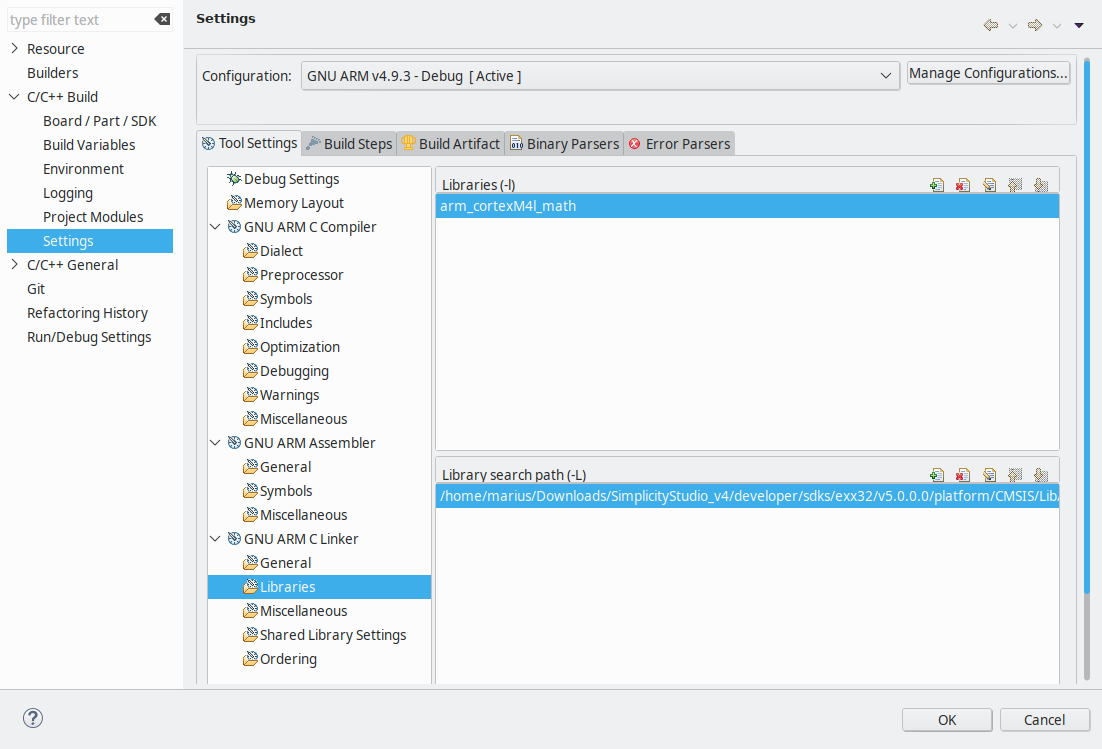
\includegraphics[width=0.85\textwidth, keepaspectratio]{imatges/EnablingDSP_Lib.png}
 \caption{Configuració del Simplicity Studio afegint-hi la biblioteca CMSIS-DSP}
 \label{fig:EnableDSP}
\end{figure}

La documentació de la biblioteca proporciona totes les funcions implementades així com un conjunt d'exemples dels usos més comuns \cite{CORE-DSP}. SiliconLabs també proporciona documentació en un {\em Application Note} sobre la biblioteca \cite{AN0051}.

\chapter{C++ vs C}
\label{ch:CvsCPP}
En aquest llibre s'ha treballat exclusivament en llenguatge C (versió C99) i no s'ha parlat res de C++. Anem a fer-ho ara en aquest capítol.

La discussió sobre usar o no C++ en sistemes encastats deu ser tant antiga com l'aparició d'aquest llenguatge orientat a objectes. Si bé als seus inicis el llenguatge presentava força problemes, ja fa molts anys que és un llenguatge estable i candidat a ser usat en sistemes encastats. Tot i això, la seva popularitat ha estat desigual i encara hi ha molts equips de desenvolupadors de sistemes encastats que treballen exclusivament en C.

Els problemes habituals que s'ha acusat al C++ per no fer-lo servir en sistemes encastats són els següents \cite{CXX_1}:
\begin{itemize}
 \item codi més llarg: si bé això pot ser veritat, les mides de les memòries \gls{FLASH} dels microcontroladors és cada cop més gran i els compiladors moderns generen codi força optimitzat, a més que es poden desactivar opcions del llenguatge que no es fan servir.
 \item més lent: això era cert amb els primers compiladors de C++, però actualment el codi generat és de la mateixa qualitat que el generat pels compiladors de C.
 \item més {\em stack}: seguint les mateixes normes que amb C, és possible tenir codi C++ que faci un ús correcte de l'{\em stack}
\end{itemize}

En canvi, els avantatges que ens pot proporcionar treballar amb C++ poden ser:
\begin{itemize}
 \item comprovació de tipus en temps de compilació. C és força laxe en aquest tema, i això pot conduir a errors. C++ és capaç de fer comprovacions en temps de compilació per avaluar la correcció de les conversions.
 \item {\em namespaces}, que permeten classificar i organitzar el codi d'una forma intuïtiva i senzilla.
 \item constructors i destructors permeten inicialitzar i destruir o netejar estructures de forma automàtica.
 \item orientació a objectes, l'organització del codi en objectes pot ajudar a ordenar i simplificar el codi.
 \item sobrecàrrega d'operadors, fent que operacions entre objectes sigui senzilla amb un codi resultant força senzill.
\end{itemize}

També cal recordar que no cal fer servir totes les noves capacitats de C++ respecte a C de cop, si no que es poden anar incorporant poc a poc al nostre codi conforme anem guanyant experiència i coneixements.

Dues de les característiques de C++ que ocupen força memòria són el \gls{RTTI} i el control d'excepcions. RTTI dona informació del tipus de classes polimòrfiques (que tenen almenys un mètode virtual) i és una característica que es faci servir gaire en sistemes encastats. El control d'excepcions permet l'execució d'un mètode i capturar l'error que es pugui generar i tractar-lo fora de la funció i de forma controlada.

Aquestes dues característiques de C++ afegeixen força codi a qualsevol projecte amb el que treballem, fent que, per exemple, no puguem compilar un simple ``Hello World embedded'' per la nostra placa de desenvolupament ja que ocupa massa FLASH. Les opcions per deshabilitar aquestes funcions al compilador GNU (que és el compilador utilitza Simplicity Studio) son:
\begin{verbatim}
-fno-rtti -fno-exceptions
\end{verbatim}

\begin{figure}
 \centering
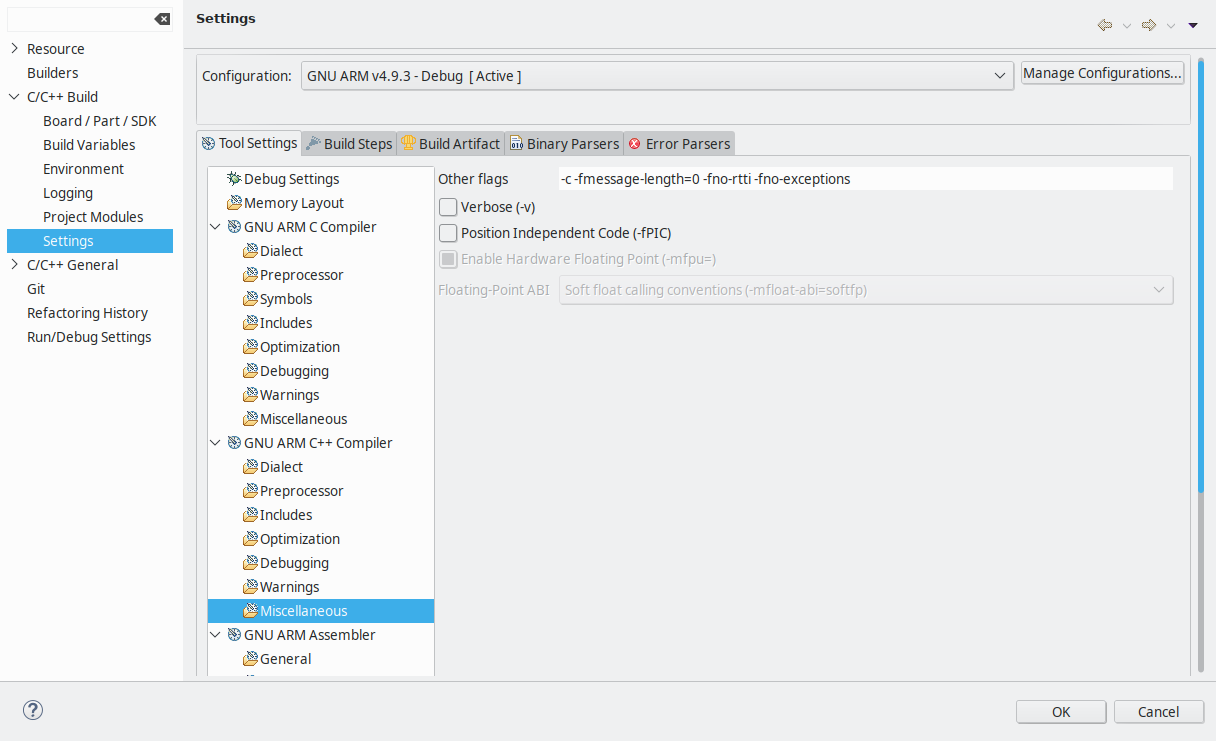
\includegraphics[width=0.85\textwidth, keepaspectratio]{imatges/CXX_options.png}
 \caption{Configuració Simplicity Studio per deshabilitar RTTI i les excepcions}
 \label{fig:CXX_RTT}
\end{figure}
i es configura tal com es veu a la Figura~\ref{fig:CXX_RTT}.

\section{Primer exemple en C++}
\label{sec:CXX_example}
\href{https://github.com/mariusmm/cursembedded/tree/master/Simplicity/CXX_1}{L'exemple CXX\_1} és el típic ``Hello World'' per sistemes encastats escrit en C++.

Aquest exemple fa servir dues classes dins el {\em namespace} {\bf BSP}.

\subsection{LED}
Com el seu nom indica, serveix per controlar l'únic \gls{LED} de la \gls{PCB} de prototipat. Està basada en una classe amb tres mètodes senzills per controlar un sol LED (LED::On(), LED::Off(), LED::Toggle())\index{LED::On()}\index{LED::Off()}\index{LED::Toggle()}.
Dins el constructor s'activa el rellotge pel perifèric \gls{GPIO} i es configura el pin corresponent al LED de la PCB (Llistat~\ref{LED_class}).

 \begin{lstlisting}[caption={Part del codi de la classe LED},style=customc,label=LED_class]
LED::LED() {
  CMU_ClockEnable(cmuClock_GPIO, true);
  GPIO_PinModeSet(gpioPortD, 7, gpioModePushPullDrive, 0); /* LED */
}
...
void LED::On() {
  GPIO_PinOutSet(gpioPortD, 7);
}
\end{lstlisting}


\subsection{Button}
Aquesta classe gestiona el valor d'una entrada del \gls{GPIO} d'una fora senzilla, la classe {\bf Button} emmagatzema els paràmetres d'un pin d'E/S i abstreu les crides a la biblioteca {\bf emlib} de Silicon Labs (veure Llistat~\ref{Button_class}).

\begin{lstlisting}[caption={Part del codi de la classe LED},style=customc,label=Button_class]
Button::Button(GPIO_Port_TypeDef port, int pin, bool pull, bool pullup) {

  CMU_ClockEnable(cmuClock_GPIO, true);

  m_port = port;
  m_pin = pin;
  m_pull = pull;
  m_pullup = pullup;

  if (m_pull == false) {
    GPIO_PinModeSet(port, pin, gpioModeInput, 0);
  } else {
    if (m_pullup == true) {
      GPIO_PinModeSet(port, pin, gpioModeInputPull, 1);
    } else {
      GPIO_PinModeSet(port, pin, gpioModeInputPull, 0);
    }
  }
}

bool Button::getValue() {
  unsigned int pin_value;

  pin_value = GPIO_PinInGet(m_port, m_pin);
  if (pin_value == 0) {
    return false;
  } else {
    return true;
  }
}
\end{lstlisting}

\subsection{Un {\em Hello World} ``més C++''}
A continuació modifiquem l'exemple per donar-li una volta més i que sigui més ``estil C++'' (està al \href{https://github.com/mariusmm/cursembedded/tree/master/Simplicity/CXX_2}{repositori}). El que s'ha fet ha estat crear una nova classe {\bf Pin} que abstrau la informació d'un pin GPIO d'EFM32. La classe {\bf Button} fa servir {\bf Pin} per obtenir les característiques del GPIO a controlar.

\subsection{Mida dels executables}
\label{CXX_size}
A \href{https://github.com/mariusmm/cursembedded/tree/master/Simplicity/CXX_1}{l'exemple CXX\_1} tenim el ``Hello World embedded'' fet en C++ de manera bàsica. A \href{https://github.com/mariusmm/cursembedded/tree/master/Simplicity/CXX_2}{l'exemple CXX\_2} s'ha fet una implementació ``més C++'' amb la mateixa funcionalitat. A la Taula~\ref{tb:CXX_size} es pot veure la quantitat de memòria de tot tipus que necessiten les dues aplicacions així com l'exemple bàsic en C.

\begin{table}[!htbp]
\caption{Ocupació de memòria de ``Hello World embedded '' en C i C++ (tots els projectes compilats amb optimització -O2).}
\centering
\begin{tabular}{|c|c|c|c|}
\hline
{\bf Aplicació} & {\bf text} & {\bf data} & {\bf bss}\\
\hline
{\bf GPIO\_1} & 972 & 108 & 28 \\
\hline
{\bf CXX\_1} & 1836 & 112 & 32 \\
\hline
{\bf CXX\_2} & 2076 & 112 & 32 \\
\hline
\end{tabular}
\label{tb:CXX_size}
\end{table}

Com a curiositat, l'ús de {\em std::cout} de la biblioteca {\em iostream} i l'operador {\bf <{}<} afegeix uns 150KB de codi FLASH (!!!), fent que sigui poc recomanable o impossible de fer servir en un sistema encastat actual.

\section{Un {\em driver} en C++}
Com hem vist al llarg del llibre, bona part del codi són {\em drivers} per controlar els diferents perifèrics o dispositius del nostre sistema encastat. Si treballem en C++, caldrà que aquest {\em drivers} els fem també en C++. Veurem ara un exemple amb la \gls{UART}, escrivint un {\em driver} i un exemple igual al vist a \fullref{sec:UART_example_2}.

En \href{https://github.com/mariusmm/cursembedded/tree/master/Simplicity/CXX_UART}{aquest exemple} tenim una classe \gls{UART} que és la implementació del {\em driver} per la UART que es va veure a l'exemple de la Secció \ref{sec:UART_example_2}. Aquesta classe {\bf UART}\index{UART class} fa servir {\em buffers} circulars per emmagatzemar les dades que es reben o s'han d'enviar per la UART i té els mètodes {\bf AvailableData()}, {\bf GetData()} i {\bf SendData()}\index{UART::AvailableData()}\index{UART::GetData()}\index{UART::SendData()} com ja tenia el mòdul UART de l'exemple en C. Aquests mètodes tant sols accedeixen al {\em buffer} circular adequat (de transmissió o recepció) que està implementat a la classe {\bf CircularBuffer} \index{CircularBuffer class}.

Tal com es veu al Llistat~\ref{operator_UARTCXX} s'ha sobrecarregat l'operador {\bf<{}<} per fer més fàcil l'ús de la classe a l'hora d'enviar dades i poder escriure codi com el del Llistat~\ref{operator_UARTCXX_example}.

\index{UART::<{}<}
\begin{lstlisting}[style=customc,caption=Ús de l'operador <{}< de la classe UART,label=operator_UARTCXX_example]
  my_uart << "Testing" << " C++ string style";
\end{lstlisting}


\index{UART::<{}<}\index{UART class}\index{UART::Tx()}
\begin{lstlisting}[style=customc,caption=Implementació de l'operador <{}< per la classe UART,label=operator_UARTCXX]
class UART {
  ...
  UART& operator<<(char* str) {
    for(char* it = str; *it; ++it) {
      this->Tx(*it);
    }
    return *this;
  }

  UART& operator<<(std::string str) {
    for(std::string::iterator it = str.begin(); it != str.end(); ++it) {
      this->Tx(*it);
    }
    return *this;
  }
  ...

  void UART::Tx(unsigned char c) const {
    USART_Tx(m_uart, c);
  }
  ...
}

\end{lstlisting}

La resta del codi és prou autoexplicatiu a excepció de l'implementació de les \glspl{ISR} de la UART. En aquest cas ens trobem que les \glspl{ISR} haurien d'estar encapsulades dins la pròpia classe UART\index{UART class} però això no és possible, donat que la classe no és estàtica, i per tant ``no existeix'' fins que no es crea instanciant un objecte d'aquest tipus \cite{ISRCXX}\cite{ISRCXX_2}. Una possible solució a aquest problema és el que es veu al codi~\ref{ISR_UARTCXX}: es té el codi pròpiament dit de la \gls{ISR} a uns mètodes privats de la classe del {\em driver} (en aquest cas la classe UART) i en algun altre lloc del codi (en aquest exemple al fitxer {\em main}\index{main()}) s'insereix la construcció que es veu al Llistat~\ref{main_ISR_UARTCXX}. D'aquesta manera les \glspl{ISR} criden als mètodes adequats de la classe pertinent.

\index{UART::USART1\_TX\_IRQHandler()}\index{UART::USART1\_RX\_IRQHandler()}\index{UART class}
\begin{lstlisting}[style=customc,caption=Implementació de les ISRs en C++,label=ISR_UARTCXX]
void UART::USART1_TX_IRQHandler(void) {
  USART_IntClear( USART1, USART_IEN_TXC);
  Send();
}

void UART::USART1_RX_IRQHandler(void) {
  char data;

  if (USART1->IF & LEUART_IF_RXDATAV) {
    data = USART_Rx(USART1);
    m_RX.PushData(data);
    USART_IntClear( USART1, USART_IEN_RXDATAV);
  }
}

class UART {
  ...
  friend void USART1_TX_IRQHandler();
  friend void USART1_RX_IRQHandler();

private:
  void USART1_TX_IRQHandler(void);
  void USART1_RX_IRQHandler(void);
  ...
}
\end{lstlisting}

\index{USART1\_TX\_IRQHandler()}\index{USART1\_RX\_IRQHandler()}\index{UART class}
\begin{lstlisting}[style=customc,caption=Part del fitxer UART.cpp de l'exemple d'us del {\em driver} en C++ per la UART,label=main_ISR_UARTCXX]
static UART* helper_uart;

void USART1_TX_IRQHandler() {
  helper_uart->USART1_TX_IRQHandler();
}

void USART1_RX_IRQHandler() {
  helper_uart->USART1_RX_IRQHandler();
}
\end{lstlisting}

\subsection{Ocupació de memòria}
De nou, anem a analitzar l'espai de memòria necessari per aquest exemple comparat amb l'exemple escrit en C amb la mateixa funcionalitat.

El codi en C++ es compila amb 3 variants:
\index{UART::<{}<}
\begin{itemize}
 \item Sobrecarregant l'operador {\bf <{}<} que pugui rebre dades de tipus {\em char}.
 \item Sobrecarregant l'operador {\bf <{}<} que pugui rebre dades de tipus {\em std::string}.
 \item Sense sobrecarregar l'operador.
\end{itemize}

Els resultats es mostren a la Taula~\ref{tb:UAR_CXX_size_O2}. Es pot veure que l'ús de l'operador que suporta {\em std::string} afegeix força codi ROM (segona columna a la Taula, uns 2 KB) i que, en general, l'ús de C++ afegeix un sobrecost en espai ROM al nostre codi. Potser el més destacable és que la quantitat de RAM necessària no s'incrementa de manera significativa, sent aquest recurs el més escàs en un microcontrolador.

% \begin{table}[!htbp]
% \caption{Ocupació de memòria d'exemple amb la UART en C i C++ (tots els projectes compilats sense optimització -O0).}
% \centering
% \begin{tabular}{|c|c|c|c|}
% \hline
% {\bf Aplicació} & {\bf text} & {\bf data} & {\bf bss}\\
% \hline
% {\bf Sense operador <{}<} & 5436 & 120 & 40 \\
% \hline
% {\bf Amb operador <{}< i char} & 5452 & 120 & 40 \\
% \hline
% {\bf Amb operador <{}< i std::string} & 7812 & 128 & 168 \\
% \hline
% {\bf Original C} & 4424 & 116 & 184\\
% \hline
% \end{tabular}
% \label{tb:UAR_CXX_size_O0}
% \end{table}

\begin{table}[!htbp]
\caption{Ocupació de memòria d'exemple amb la UART en C i C++ (tots els projectes compilats amb optimització -O2, en KB).}
\centering
\begin{tabular}{|l|c|c|c|}
\hline
{\bf Aplicació} & {\bf text} & {\bf data} & {\bf bss}\\
\hline
{\bf Sense operador <{}<} & 4636 & 120 & 40 \\
\hline
{\bf Amb operador <{}< i char} & 4644 & 120 & 40 \\
\hline
{\bf Amb operador <{}< i std::string} & 6796 & 128 & 168 \\
\hline
{\bf Original en C} & 2620 & 116 & 184\\
\hline
\end{tabular}
\label{tb:UAR_CXX_size_O2}
\end{table}





\section{Conclusions}
Tot i que l'ús de C++ enlloc de C incrementa la mida de l'executable final i les seves necessitats de memòria, el seu ús pot estar justificat en casos on l'encapsulació que proporciona C++ ajudi a la claredat del codi o a la portabilitat del mateix a diferents plataformes.

En qualsevol cas, cal una expertesa en el llenguatge per fer-ne un bon ús per tenir en compte les particularitats d'escriure codi C++ per sistemes encastats.


\chapter{Relació Esquemàtic i FW}
\label{ch:schematic}
Quan es dissenya un sistema encastat, una de les parts més importants i on contribueixen perfils professionals de diferent mena és la del disseny de l'esquemàtic. Aquest document especifica tots els detalls hardware de la connexió dels dispositius del sistema, els diferents dominis d'alimentació, els diferents rellotges del sistema, etc. Tots aquests aspectes influiran i seran influïts per, entre d'altres, el disseny de \gls{FW} i les característiques particulars del microcontrolador triat. És per tot això que en aquesta primera fase de disseny, cal implicació de part de l'equip de \gls{FW}.

\section{Selecció de pin-out}
Els microcontroladors actuals tenen la capacitat de poder cablejar la sortida o entrada d'un dels perifèrics a diferents pins del mateix. Per exemple, els dos pins del bus I2C (SCL i SDA, veure \fullref{sub:I2C}), en cert dispositiu de Silicon Labs (EFM32TG840) es poden cablejar cap a: PA0/PA1, PD6/PD7, PC6/PC7, PF0/PF1, PE12/PE13 \cite[50]{EFM32TG840}. A nivell de \gls{FW} serà indiferent fer servir un o altre conjunt de pins (tant sols caldrà canviar la configuració) però a nivell d'esquemàtic i a l'hora de fer la \gls{PCB} pot ser un canvi important.

Un altre aspecte a tenir en compte serà el dels pins d'entrada que poden o no generar \gls{IRQ}, de quina mena, etc. Per exemple, ja s'ha comentat que a la família STM32 de ST, els pins amb el mateix nombre generen la mateixa interrupció, així el pin PE6 genera la mateixa interrupció (EXTI6) que el pin PA6 \cite[382]{STM32F4RM}. De forma similar, a EFM32 els pins generen una interrupció o una altra segons tinguin numeració parell o senar i només un pin de cada conjunt amb el mateix nombre pot generar interrupció (només un dels pins de cada conjunt pot generar \gls{IRQ}: PA1, PB1, PC1, PD1, etc.) \cite[471]{EFM32TGRM}. Aquestes particularitats de cada família poden ser un inconvenient pel disseny \gls{FW} del sistema i caldrà tenir-ho en compte alhora de dissenyar l'esquemàtic i el \gls{FW} associat.

\section{Selecció de rellotges}
Un altre aspecte important és el de triar la freqüència de funcionament del rellotge del sistema i d'altres rellotges auxiliars. Com ja s'ha comentat a \fullref{ch:low-power}, la freqüència de funcionament del sistema és un dels factors més importants en el consum del microcontrolador. Com és evident, també afecta de forma directa al rendiment del sistema i a la seva capacitat de càlcul, procés de dades i resposta a esdeveniments.

També, però, és important la freqüència triada per la generació d'altres freqüències que necessitin alguns perifèrics. Per exemple, la USART necessita certes freqüències de rellotge per poder treballar amb els {\em bit-rates} més habituals. Els fabricants proporcionen mètodes per calcular les millors opcions de freqüències segons el {\em bit-rate} desitjat o taules amb paràmetres precalculats \cite[153]{EFM32TGRM} \cite[980]{STM32F4RM}.

Cal tenir en compte que, sovint, els microcontroladors tenen més d'un arbre de rellotges (veure \fullref{sec:clocks}) i que cal triar bé quins oscil·ladors i a quina freqüència treballaran.

\section{Canvis durant el {\em layout}}
Per últim, succeeix sovint que certes connexions de l'esquemàtic es canvien en l'etapa de \gls{layout} per necessitats del disseny. Pot ser que per poder {\em routejar} millor una línia es demani de canviar de pin. Això provocarà canvis en el \gls{FW} que s'hauran de tenir en compte. Si hem fet bé el disseny del nostre codi, només caldrà fer algun canvi senzill al nostre \gls{BSP} (veure \fullref{sec:BSP}).

\section{De la placa de prototipat a PCB pròpia}
Un altre dels canvis importants és el de passar de treballar amb una placa de prototipat o de desenvolupament a poder-ho fer en una PCB pròpia. La placa de prototipat porta muntat cert nombre de dispositius externs que segurament no estaran presents a la nostra PCB.

\subsection{Mecanisme de programació}
Un dels canvis més notoris és de l'absència del programador integrat a la PCB pròpia. Les plaques de desenvolupament modernes acostumen a integrar el programador, de manera que la placa de prototipat s'alimenta i es programa a través d'un connector USB estàndard. Això amaga que a la pròpia placa de desenvolupament hi ha tota el circuit per programar el microcontrolador principal. De fet, a la placa de prototipat que estem fent servir, hi ha un microcontrolador que rep les comandes del {\em debugger} per USB i les transforma a les comandes adequades per programar el microcontrolador principal a través del port {\em SWD} \cite[30]{USERMANUALDEVKIT}.

Aquest circuit no s'acostuma a posar les PCBs de productes finals, si no que es deixa disponible d'alguna manera (connector, pins, {\em pads}) a la PCB l'accés directe al port {\em SWD} del microcontrolador. Això provoca que calgui un programador extern a la PCB per tal de poder programar el microcontrolador. Això es pot fer comprant un dispositiu {\em debugger}, tot i que també es pot fer servir una de les plaques de prototipat perquè faci de programador de qualsevol microcontrolador extern connectat a través del port de DEBUG.

A part d'aquesta mena de programació pel port SWD, es pot tenir en compte que alguns microcontroladors porten un {\em bootloader} en HW que permet actualitzar el Firmware via un port sèrie (veure \fullref{sec:Bootloader}) \cite{AN0003}. Això pot simplificar la programació del microcontrolador, però cal tenir en compte que aquesta mena de comunicació no permet {\em debug}. 

% \subsection{BSP}
% Com ja s'ha comentat prèviament (\fullref{sec:BSP}), l'ús d'un BSP permetrà canviar els ports i pins dels diferents perifèrics sense haver de canviar codi arreu del projecte.

\subsection{Migració vertical}
Treballant amb la placa de prototipat es poden avaluar les prestacions del sistema així com les necessitats de memòria, tant \gls{FLASH} com \gls{RAM}. Usualment, i per temes de costos, s'acostuma a triar el microcontrolador de la mateixa família més senzill i barat que compleixi els requeriments trobats.

Aquest canvi també pot causar canvis al nostre \gls{FW}, ja que pot ser que diferents models tinguin un mapat de pins diferents, o algun perifèric no es pugui {\em routejar} al pin que s'havia previst, etc. Aquesta informació acostuma a estar al {\em Reference Manual} de cada família, a \cite[8]{EFM32TGRM} es veu la taula resum de cada model (anomenats {\em parts} en anglès).

Per migració vertical ens refereix a la possibilitat de canviar de família dins un mateix fabricant mantenint el mateix encapsulat físic de manera que es poden incrementar les capacitats del microcontrolador sense haver de fer canvis a la \gls{PCB}.
Per exemple, es pot consultar els {\em datasheets} de la família {\em Tiny Gecko} (Cortex-M3) \cite[72]{EFM32TGDS}, {\em Zero Gecko} (cortex-M0+) \cite[66]{EFM32ZGDS} i {\em Happy Gecko} (Cortex-M0+)\cite[76]{EFM32HGDS} i es veurà que el mateix encapsulat, per exemple un QFN24, és compatible pin a pin amb qualsevol de les tres famílies (veure Figura~\ref{fig:pinout}). Així, en el nostre disseny podrem posar un Cortex més potent o menys segons l'aplicació o les necessitats sense haver de canviar el dibuix de la PCB. El mateix passa amb altres encapsulats i models tant en aquesta fabricant com a d'altes.

Com que actualment les biblioteques que ofereixen són compatibles entre diferents famílies (o si més no, molt similars) la transició entre diferents famílies acostuma a ser força senzill. La biblioteca {\bf emib} no presenta canvis entre diferents famílies de Cortex, per tant el nostre codi no haurà de recollir cap canvi en aquest sentit.

\begin{figure}[b]
 \centering
 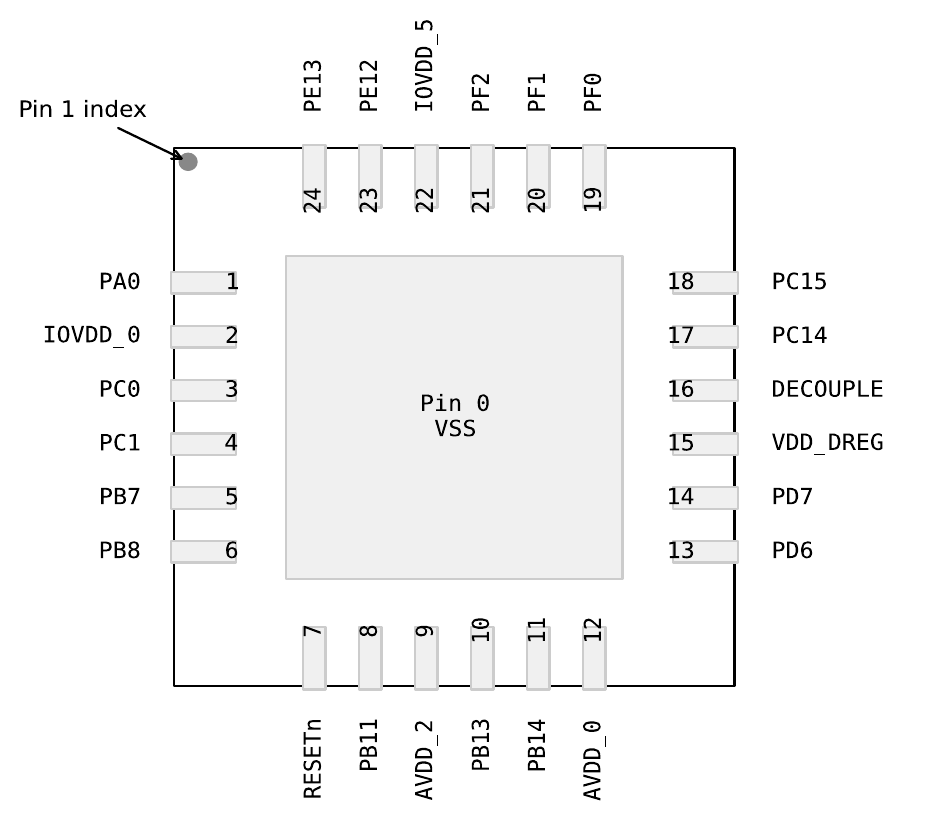
\includegraphics[width=0.65\textwidth, keepaspectratio]{imatges/pinout.png}
 \caption{Pinout pels microcontroladors EFM32ZG, EFM32HG i EFM32TG amb encapsulat QFN24 (extret de \cite[72]{EFM32TGDS}).}
 \label{fig:pinout}
\end{figure}




%----------------------------------------------------------------------------------------
% 6a Part: Temes avançats
%----------------------------------------------------------------------------------------s
\part{Temes avançats}
\label{part:avançats}
% \part{Temes avançats}
% \label{part:avançats}

\chapter{Gestió d'excepcions}
\label{ch:exceptions}
Sovint treballant amb sistemes encastats ens trobem amb errors d'origen desconegut que es poden provocar per múltiples causes. Així, per exemple, una divisió per zero, un accés incorrecte a una zona de memòria o un accés a una posició de memòria fora de rang faran que el processador es reiniciï \cite[102]{DesignersGuide}\cite[318]{ARMsdg}\cite{KielHardFault}.

Aquests casos poden ser molt difícils de trobar si són casos esporàdics, però l'arquitectura ARM té unes característiques que ajuden a detectar-los i trobar-los. En síntesi, el cortex-M llença una interrupció molt prioritària anomenada {\bf HardFault\_Handler()}\index{HardFault\_Handler()} quan succeeix un problema greu del que el processador no pot recupera-se, com una divisió per zero, un accés il·legal a memòria, etc. Abans de cridar a l'excepció, la CPU guarda tot de valors claus a diferents registres, i així per exemple en el registre {\bf PC} s'hi emmagatzema l'adreça de la instrucció executada, així que, en principi, només cal anar a aquella posició de memòria per veure quin ha estat el codi que ha causat el problema. També s'emmagatzema el valor de retorn (la  instrucció següent a l'executada que ha causat l'error) al registre {\bf LR} \cite{BlogHardFalut}.

Així doncs, es pot reescriure la ISR per obtenir les dades que ens informi sobre què ha passat per ajudar-nos a obtenir pistes de quin codi està fallant \cite{ARMHandler}.

\section{Exemple detectant errors greus}
A l'\href{https://github.com/mariusmm/cursembedded/tree/master/Simplicity/ErrorHandling}{exemple del repositori} hi ha un codi que genera diferents errors segons la funció que es cridi i una implementació de {\bf HardFault\_Handler()}\index{HardFault\_Handler()}. Aquesta funció està escrita en assemblador, però el que cal veure és que es crida a la funció {\bf my\_HardFault\_Handler()}\index{my\_HardFault\_Handler()} que es qui en realitat fa tota la feina i és la que cal entendre \cite{EFM32HardFault}.

\index{my\_HardFault\_Handler()}
\begin{lstlisting}[style=customc,caption=Codi HardFault\_Handler,label=HardFaultHandler_1]
void my_HardFault_Handler(uint32_t *stack) {
  printf("Error Handler\r\n");
  printf("SCB->HFSR = 0x%08lx\r\n", (uint32_t) SCB->HFSR);

  if ((SCB->HFSR & (1 << 30)) != 0) {
    printf("Forced Hard Fault\r\n");
    printf("SCB->CFSR = 0x%08lx\r\n", SCB->CFSR);

    if ((SCB->CFSR & 0x02000000) != 0) {
      printf("Divide by zero\r\n");
    }
    if ((SCB->CFSR & 0x01000000) != 0) {
      printf("Unaligned\r\n");
    }
    if ((SCB->CFSR & 0x00010000) != 0) {
      printf("Undefined\r\n");
    }
  ...
}
\end{lstlisting}

A la primera part (veure Llistat~\ref{HardFaultHandler_1}) de la \gls{ISR} es treu per la consola de {\em debug} la causa de l'excepció ({\em bus fault}, {\em memory access}, {\em divide by zero}, etc.).

Tot seguit es treu per la mateixa consola els valors dels registres que hi ha a l'\gls{stack} per tenir dades que ens permetin localitzar l'error (Llistat~\ref{HardFaultHandler_2}).

\begin{lstlisting}[style=customc,caption=Codi HardFault\_Handler (continuació),label=HardFaultHandler_2]
void my_HardFault_Handler(uint32_t *stack) {
  ...
  printf("sp = 0x%08lX\r\n",  (uint32_t) stack);
  printf("r0 = 0x%08lX\r\n",  stack[0]);
  printf("r1 = 0x%08lX\r\n",  stack[1]);
  printf("r2 = 0x%08lX\r\n",  stack[2]);
  printf("r3 = 0x%08lX\r\n",  stack[3]);
  printf("r12 = 0x%08lX\r\n", stack[4]);
  printf("lr = 0x%08lX\r\n",  stack[5]);
  printf("pc = 0x%08lX\r\n",  stack[6]);
  printf("psr = 0x%08lX\r\n"  stack[7]);
  ...
}
\end{lstlisting}


\begin{figure}
 \centering
 \fbox{\color{ocre}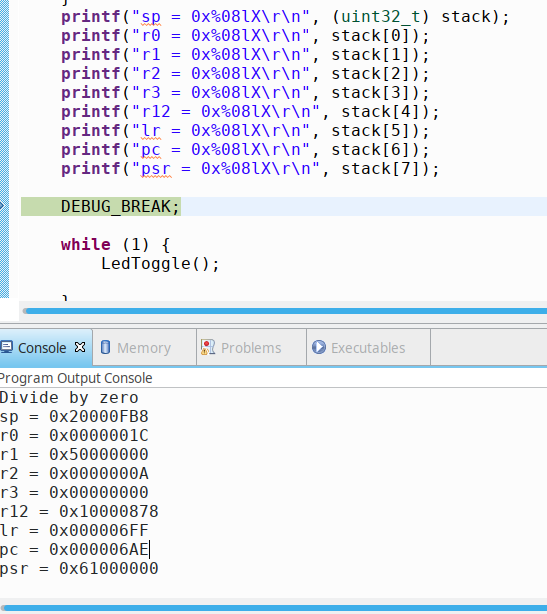
\includegraphics[width=0.65\textwidth, keepaspectratio]{imatges/HardFault_Console.png}}
 \caption{Debugger aturat a la instrucció DEBUG\_BREAK i el {\em dump} els registres}
 \label{fig:HardFaultDump}
\end{figure}


Per últim, es crida la macro {\bf DEBUG\_BREAK}\index{DEBUG\_BREAK}, que està definida com una instrucció en assemblador ({\bf BKPT \#01}) que posa el {\em core} en mode {\em Debug} i atura l'execució en aquest punt. Així, si tenim un {\em debugger} connectat, veurem com l'execució s'atura en aquest punt i torna el control a la nostra eina (veure Figura~\ref{fig:HardFaultDump}).


\begin{figure}
 \centering
 \fbox{\color{ocre}\includegraphics[width=0.65\textwidth, keepaspectratio]{imatges/HardFault_Dissassembly.png}}
 \caption{Codi assemblador a la posició de memòria indicada pel registre {\bf PC}}
 \label{fig:HardFaultDis}
\end{figure}

Si anem a la finestra {\em Disassembly} i anem a la posició de memòria que indica el registre {\bf PC} (0x6AE a l'exemple), veurem que apunta a una instrucció assemblador {\em sdiv}, que es corresponent amb una divisió. Si mirem el codi anterior, podem deduir que a la posició de memòria {\bf R7+0x8} (corresponent a la variable {\em b}) s'hi ha emmagatzemat un 0 (instruccions a 0x6A6 i 0x6A8) i aquesta variable es fa servir a la divisió com a divisor, causant l'error (veure Figura~\ref{fig:HardFaultDis}).

També cal comentar que les diferents funcions que generen errors són les següents:
\begin{itemize}
 \item {\bf WrongfunctionDiv0()}\index{WrongfunctionDiv0()} causa una divisió per zero.
 \item {\bf WrongfunctionAlign()}\index{WrongfunctionAlign()} causa un error d'accés a memòria fora d'alineament.
 \item {\bf WrongfunctionWrongMemory()}\index{WrongfunctionWrongMemory()} causa un error per accés fora dels límits de la memòria.
 \item {\bf fp()}\index{fp()} causa un intent d'executar a la posició 0x0000\_0000 de memòria.
\end{itemize}

\chapter{{\em Shadow Registers}}
En algunes arquitectures i en perifèrics d'alguns fabricants poden llegir que es fan servir {\em shadow registers}. S'anomenen així a registres que contenen una còpia d'un altre registre i que son els que es poden llegir per part d'altres dispositius o perifèrics. 

Així per exemple, trobem {\em shadow registers} a alguns processadors de manera que quan la CPU entra a una interrupció es passa a treballar amb un banc separat de registres de propòsit general. Això es fa per evitar un sobrecost a la crida de la ISR, ja que si es tenen aquests registres s'han de guardar els valors actuals de tots els registres a la pila abans de poder executar el codi de la ISR. En canvi, si es tenen aquests registres, la CPU passa a treballar amb un banc diferent (els {\em shadow registers}) durant l'execució de la ISR i no cal salvaguardar cap valor dels registres originals. Un cop se surt de la ISR la CPU torna a treballar amb el banc de registres originals. En el cas dels Cortex-M no es treballa amb aquesta mena de {\em shadow registers} i, per tant, caldrà que les ISR salvin els valors dels registres de propòsit general que sobreescriguin durant la seva execució.

Una altra lloc on ens podem trobar {\em shadow registers} és en alguns perifèrics que treballen valors grans repartits en diversos registres. Si aquests registres s'actualitzessin entremig d'una lectura per part del Firmware, aquest podria tenir una inconsistència a les dades. Per això, és habitual que un valor determinat s'emmagatzemi a {\em shadow registers} mentre els registres ``amagats'' s'actualitzen de forma normal. Aquests {\em shadow registers} seran els que el firmware pot llegir i s'actualitzaran tots de cop una vegada s'hagin llegit tots pel firmware. 

\begin{remark}
 A tots ens ha passat o tenim un company que ha perdut una tarda sencera intentant llegir uns registres d'aquesta mena sense seguir bé l'ordre i rebent valors dolents sense caure en el problema amb els {\em shadow registers}.
\end{remark}

Un exemple d'això últim succeeix amb els registres de data i temps del RTC dels microcontroladors d'ST (veure~\fullref{sub:RTC}). Aquest perifèric conté uns {\em shadow registers} on es copien cada 2 cicles els registres reals amb la data, el temps i els segons del RTC (Figura~\ref{fig:ShadowRegisters}). Quan es llegeix el registre amb el temps o amb els segons es bloqueja la còpia de tots els tres registres perquè la lectura dels demès no doni cap incoherència. Si no hi fossin, podria passar que es llegís el temps (per exemple les 23:59:59 del dia 1) i poc després al llegir la data ja hagués passat el segon i la data ja fos el dia 2, resultant en que enlloc de llegir les 23:59:59 del dia 1 s'hauria llegir les 23:59:59 del dia 2. En aquest cas sembla que és molt millor llegir la data correcte i que es tingui un error d'un segon a tenir un dia sencer d'error (!).

Per tant, en aquest perifèric, primer cal llegir el registre amb el temps o els segons i després el registre amb la data \cite[800-805]{STM32F4RM}. Així si només es vol llegir el temps del RTC perquè no interessa la data del sistema, no es poden fer lectures consecutives del temps sense llegir també, encara que no interessi, la data del RTC. La API del fabricant en aquest cas no ho gestiona, però si que ho adverteix a la seva documentació \cite[719]{STM32UM1725}.

\begin{figure}
 \centering
 \includegraphics[width=0.65\textwidth, keepaspectratio]{imatges/ShadowRegisters.png}
 \caption{{\em Shadow registers} del perifèric RTC dels STM32 \cite[800]{STM32F4RM}}
 \label{fig:ShadowRegisters}
\end{figure}


\chapter{Baix cosum}
\label{ch:low-power}
Un dels temes més habituals de trobar-se quan es tracten temes amb microcontroladors és el del baix consum. Gràcies a la tecnologia de fabricació dels microxips i els avenços en les arquitectures dels microcontroladors, aquests han arribat a unes fites de consum molt baixes, permeten desenvolupar aplicacions on el sistema pugui anar alimentat per bateries o altres fonts d'alimentació alternatives a l'alimentació general. En aquest capítol veurem les característiques actuals dels microcontroladors en aquest aspecte, com treure tot el partit a aquestes característiques i, per últim, com adaptar els \gls{RTOS} per treballar amb baix consum.

Cal repassar uns quants conceptes sobre el consum d'energia abans d'introduir-nos de ple en el tema.

\section{Consideracions prèvies}
\label{sec:lowpowerintro}

Per la pròpia natura dels circuits digitals, aquests consumeixen sobretot quan el seu rellotge principal està actiu. Això fa que l'estratègia principal per reduir el consum d'un circuit és desactivar-li precisament el rellotge o reduir la seva freqüència, ja que el consum és proporcional a la velocitat de rellotge.
\begin{remark}
 Donat que el consum és quasi proporcional a la freqüència de rellotge, els fabricants acostumen a donar el consum per MHz (típicament $\mu$A/MHz).
\end{remark}

També cal tenir en compte que qui més consumeix en un microcontrolador és el propi {\em core} o CPU i que, per tant, serà el mòdul que caldrà tenir apagat el màxim de temps possible.

\section{Modes d'{\em sleep}}
\label{sec:sleepmodes}
Els diferents fabricants de microcontroladors basats en Cortex-M ofereixen diferents modes d'sleep, això és, diferents combinacions de perifèrics que estan actius a cada mode per tal de reduir el consum.

Així, els microcontroladors de Silicon Labs tenen 4 modes d'sleep\footnote{A més, hi ha el mode normal, on la CPU està a ple rendiment} \cite[6]{EFM32GRM}:
\begin{itemize}
 \item EM0 - {\em Energy Mode 0}: Tot el sistema està actiu incloent-hi tots els perifèrics.
 \item EM1 - {\em Energy Mode 1}: La CPU està desactiva i la resta de perifèrics estan disponibles.
 \item EM2 - {\em Energy Mode 2}: La CPU està desactivada i només els perifèrics de baix consum estan disponibles (UART, RTC, TIMER, Watchdog)
 \item EM3 - {\em Energy Mode 3}: Tot el sistema està desactivat, només es manté la RAM activada i certes interrupcions
 \item EM4 - {\em Energy Mode 4}: Tot el sistema està desactivat, només es pot fer un {\em reset} al sistema.
\end{itemize}

En canvi, els microcontroladors de ST tenen només 3 modes de baix consum\footnote{Versions de Cortex-M0+ tenen algun mode més} \cite[126]{STM32F4RM}:
\begin{itemize}
 \item {\em Run mode}: Tot el sistema està actiu incloent-hi tots els perifèrics.
 \item {\em Sleep mode}: La CPU està desactiva i la resta de perifèrics estan disponibles.
 \item {\em Stop mode}: Tot el sistema està desactivat, només es manté la RAM activada i certes interrupcions
 \item {\em Standby mode}: Tot el sistema està desactivat, només es pot fer un {\em reset} al sistema.
\end{itemize}

\begin{table}
\caption{Consum d'energia de diferents fabricants i modes (per un Cortex-M0+) \cite{EFM32ZG108DS}\cite{STM32L01}}
\centering
\begin{tabular}{|c|c|c|}
\hline
{\bf Processador} & {\bf STM32} & {\bf EFM32}\\
{\bf SleepMode} & & \\
\hline
{\bf EM0 - {\em Run mode}} &  76 $\mu$A/Mhz &  114 $\mu$A/MHz\\
\hline
{\bf EM1 - {\em Sleep mode}} & ~42  $\mu$A/MHz & 48 $\mu$A/MHz\\
\hline
{\bf EM4 - {\em Standby mode}} & 230 nA & 20 nA \\
\hline
\end{tabular}
\label{tb:bin_size}
\end{table}

Els {\em core} Cortex-M es poden posar en mode de baix consum fent servir dues instruccions {\bf WFI} i {\bf WFE}. El primer que cal fer és configurar a quin mode d'adormir es vol posar el microcontrolador i després executar la instrucció que pertoqui. La CPU es quedarà en l'estat de baix consum que s'hagi configurat fins que es generi una \gls{IRQ} per algun perifèric o generat per un senyal extern.

\section{Estratègies de baix consum}
\label{sec:lowpowerstrategies}
Vist tot l'anterior, l'estratègia bàsica per tenir un baix consum serà la de preparar els perifèrics per a que facin la funcionalitat d'entrada/sortida necessària de manera que llencin una \gls{IRQ} quan finalitzin, posar en un dels modes de baix consum on la CPU està desactivada a l'espera de les interrupcions; a continuació, la CPU processarà les dades o esdeveniments que hagin succeït i es tornarà a configurar els perifèrics i es tornarà a posar la CPU en mode baix consum, etc.

Per tant, quan es desenvolupa una aplicació per ser de baix consum, s'acostuma a treballar basant-se en interrupcions (Veure~\fullref{ch:IRQ}) i tenint la CPU el màxim de temps en algun dels modes de baix consum.

\subsection{Exemple de baix consum}
\href{https://github.com/mariusmm/cursembedded/tree/master/Simplicity/ADC_1_LP}{L'exemple que es veurà} farà servir l'\gls{ADC} per convertir una entrada analògica a un valor digital, com ja es a fer a l'exemple \fullref{sub:ADC_example}. En el cas de baix consum, es configura el perifèric de la mateixa forma però s'hi afegeix l'opció que generi una \gls{IRQ} quan acaba de fer una conversió. Així, el nostre codi al bucle principal engegarà la conversió, entrarà en el mode de baix consum {\bf EM1} perquè la CPU es quedi en repòs mentre l'ADC fa la seva feina i es desperti per la \gls{IRQ} de finalització; tot seguit es llegeix i es mostra la dada convertida.

\index{main()}\index{ADC\_Start()}\index{EMU\_EnterEM1()}\index{ADC\_DataSingleGet()}
\begin{lstlisting}[style=customc,caption={Bucle principal amb funcions de baix consum}, label=ADC_LP]
void main() {
  ...
  while (1) {
    ADC_Start(ADC0, adcStartSingle);

    EMU_EnterEM1();

    ADCvalue = ADC_DataSingleGet(ADC0);
    printf("ADC Value %lu\r\n", ADCvalue);
  }
  ...
}
\end{lstlisting}

Podem fer una mesura del temps que està la CPU en el mode EM1 posant un pin a '1' quan s'entra al mode i posar-lo a '0' quan se'n surt, tal com es veu al projecte d'exemple.

Si usem l'analitzador lògic per mesurar els temps, veiem la imatge de la Figura~\ref{fig:adc_logic} que les mesures diuen que 44,29 microsegons de 52.21 la CPU està en mode de baix consum (el 84.84\% del temps).

\begin{figure}
 \centering
 \includegraphics[width=0.85\textwidth, keepaspectratio]{imatges/ADC_LP1_Measurement.png}
 \caption{Captura de les mesures de temps amb l'analitzador lògic}
 \label{fig:adc_logic}
\end{figure}

\section{{\em Timers} de baix consum}
\label{sub:letimer_example}
Un mode que es fa servir sovint en sistemes de baix consum és el de tenir un {\em timer} configurat perquè desperti el sistema cada cert temps. Així per exemple, en un sistema que ha de llegir un sensor cada 30 segons, el {\em timer} seria l'únic perifèric en funcionament actiu i estaria configurat per generar una \gls{IRQ} cada 30 segons; la resta del microcontrolador podria estar en un mode de baix consum que el permeti consumir molt poca energia mentre espera a ser despertat per una \gls{IRQ}.

Al \href{https://github.com/mariusmm/cursembedded/tree/master/Simplicity/LETIMER_LP}{projecte del repositori} hi ha un exemple d'aquest tipus. Es fa servir un {\bf LETIMER}, que és un {\em timer} de baix consum i baixa freqüència que pot funcionar mentre la resta del microcontrolador està en el mode EM2 (o EM3 segons la configuració que es faci servir) \cite[294]{EFM32TGRM}. Aquest {\bf LETIMER} es pot alimentar amb el rellotge extern de baixa freqüència a 32.768 Hz ({\bf LFXO}) o bé amb l'oscil·lador intern a 1.000 Hz ({\bf ULFRCO}) (al codi es pot triar segons es defineixi o no la macro {\bf USE\_ULFRCO}). El rellotge que s'hagi triat es pre-escala per un factor suficient per tenir un comptador prou lent, ja que cal tenir en compte que aquest comptador és de només 16 bits i, per tant, si tenim una freqüència de funcionament elevada no podrem comptar gaire temps.
Tot seguit el {\em timer} es configura per generar una interrupció quan arribi a 0 (és un comptador decreixent) i el seu valor {\bf TOP} (al valor al que es reinicia després d'arribar a 0) es posa en funció de la freqüència de funcionament i el temps que es vol tenir el sistema en baix consum, a l'exemple del repositori es posa a 4 segons. Un resum del codi de l'exemple es veu a Llistat~\ref{LETIMER_example}.

\index{LETIMER0\_IRQHandler()}\index{main()}\index{LETIMER\_IntGet()}\index{LETIMER\_IntClear()}
\index{GPIO\_PinOutToggle()}\index{CMU\_ClockSelectSet()}\index{CMU\_ClockDivSet()}
\index{LETIMER\_CompareSet()}\index{EMU\_EnterEM3()}
\begin{lstlisting}[style=customc, caption={Exemple ús de {\bf LETIMER}}, label=LETIMER_example]
#define PRESCALER cmuClkDiv_1
#define EFECTIVE_CLK_FREQ (1000/PRESCALER)
#define SLEEP_SECONDS 4
#define TOP_VALUE (EFECTIVE_CLK_FREQ * SLEEP_SECONDS)

void LETIMER0_IRQHandler(void) {
	uint32_t flags;

	/* Clear flag for LETIMER0 */
	flags = LETIMER_IntGet(LETIMER0);
	LETIMER_IntClear(LETIMER0, flags);

	/* Toggle LED ON/OFF */
	GPIO_PinOutToggle(gpioPortD, 7);
}

void main(void) {
  ...
  /* ULFRCO is 1,000 kHz */
  CMU_ClockSelectSet(cmuClock_LFA, cmuSelect_ULFRCO);
  CMU_ClockDivSet(cmuClock_LETIMER0, PRESCALER);
  ...
  LETIMER_CompareSet(LETIMER0, 0, TOP_VALUE);
  ...
  while (1) {
    /* nothing to do here */
    EMU_EnterEM3(true);
  }
}
\end{lstlisting}

Aquest és un exemple senzill que fa servir un {\em timer} especial de la família EFM32 de Silicon Labs. Altres fabricants proporcionen {\em timers} similars. Així ST té un {\em timer} força similar, anomenat LPTIMER (\cite{ST_ANS4865}) i Fresscale te el LPTMR amb característiques similars \cite{Kinetis_LPTMR}. Els {\em timers} de ST i de Silicon Labs  poden generar senyals tipus \gls{PWM} mentre el microcontrolador està en modes de baix consum (veure \fullref{sub:PWM}).

\section{Baix consum i RTOS}
\label{sec:lowpwerRTOS}
Quan treballem amb un RTOS funcionant en el nostre microcontrolador, hi ha diferents estratègies per aconseguir disminuir el consum energètic.

Bàsicament hi ha dues estratègies:
\begin{itemize}
 \item Aprofitar la tasca {\em Idle} per posar al microcontrolador en un mode de baix consum.
 \item Passar a un sistema sense {\em tick} (també dit {\em tickless}).
\end{itemize}

En qualsevol cas, l'avantatge de que sigui el SO qui s'encarregui de gestionar el baix consum és que les tasques no s'han de preocupar per aquesta gestió.

\subsection{Tasca {\em Idle} per baix consum}
\label{sub:idlelowpower}
L'estratègia més senzilla és la d'activar un mode de baix consum quan s'executa la tasca {\em Idle}. Com que aquesta tasca s'executa quan no hi ha cap altra tasca preparada per agafar el microcontrolador, té sentit pensar en aturar el microcontrolador i esperar a que una tasca estigui disponible. Quan succeeixi el proper {\em tick}, el microcontrolador sortira del mode d'{\em sleep} i tornarà a executar el planificador, que, si segueix sense haver cap tasca disponible (en estat {\em Ready}) per executar tornarà a executar la tasca {\em Idle} que tornarà a adormir la CPU i es repetirà el cicle \cite{FreeRTOSLP}.

\begin{remark}
Cal recordar que quan el {\em core} està en algun mode de baix consum, el {\em SysTick} també es desactiva. Per tant, per poder tenir un {\em tick} quan el {\em core} està en un mode de baix consum caldrà fer servir un altre Timer que si que funcioni en aquests modes de baix consum.
\end{remark}

Cal pensar que tot i que aquest mètode és molt senzill d'implementar, té la limitació de que a cada {\em tick} es treu la CPU del mode de baix consum per comprovar si hi ha alguna tasca en estat {\em Ready}. Podem imaginar-nos una aplicació que llegeixi d'un sensor cada 200 ms i processant les dades, com l'aplicació d'exemple XXXXX. Si es té en compte que el {\em tick} pot ser de 1000 Hz, és fàcil d'observar que es despertarà molts cops al {\em core} perquè tant sols el planificador vegi que no hi ha cap tasca {\em Ready} i torni a adormir el processador.

%% manual break a la ultima macro pq latex no ho fa be
Aquesta característica es pot activar a FreeRTOS editant el fitxer ``FreeRTOSConfig.h'' i fixant a '0' la definició {\bf configUSE\_TICKLESS\_IDLE} i triant el valor '1' per {\bf configUSE\_SLEEP\_MODE\\\_IN\_IDLE}. En el cas de Silicon Labs, el microcontrolador es posa en el mode EM2 (veure \fullref{sec:sleepmodes}) i deixant en funcionament tant sols el RTC (veure \fullref{sub:RTC}) i les \gls{IRQ} dels GPIOs que l'usuari hagi configurat (veure \fullref{ch:IRQ}).

\subsection{FreeRTOS sense {\em tick}}
\label{sub:tickless}

L'altre estratègia per disminuir encara més el consum, és desactivar el {\em tick} durant cert temps. En una aplicació on totes les tasques estan bloquejades (i que entraria la tasca {\em Idle}) es pot calcular el temps en que alguna tasca es desbloquejarà (perquè alguna tasca estigui bloquejada perquè ha cridat la funció vTaskDelay()\index{vTaskDelay()}). Es pot desactivar el {\em Tick} i programar el Timer perquè generi una interrupció en aquell temps calculat. Si mentre està el sistema adormit esperant aquell temps hi ha algun esdeveniment extern (interrupció), es despertarà i es podrà reprendre l'execució normal i tornar a activar el {\em Tick}.

Amb aquesta estratègia es maximitza el temps en que el {\em core} està en algun dels modes de baix consum i per tant es pot reduir dràsticament el consum d'una aplicació (veure \fullref{ch:low-power}).

En el cas de FreeRTOS, el port disponible per Cortex-M ja incorpora aquesta característica, i es pot configurar editant el fitxer ``FreeRTOSConfig.h'', concretament fixant el valor '1' a la macro {\bf configUSE\_TICKLESS\_IDLE}. En el cas de Silicon Labs, el microcontrolador es posa en el mode EM2 igual que en cas amb {\em ticks} i es programa el RTC perquè generi una \gls{IRQ} en el temps adequat.

En ambdós casos el codi que gestiona el baix consum i els {\em ticks} en el port FreeRTOS està al fitxer {\bf low\_power\_tick\_management.c} a la funció {\bf vPortSetupTimerInterrupt()}\index{vPortSetupTimerInterrupt()}.

\chapter{Documentant el codi}
\label{sec:documentant}
Un tema recurrent en temes d'enginyeria del software és com documentar el codi font que es desenvolupa per tal d'afavorir, sobretot, el manteniment del codi durant el temps i algú altre (o nosaltres mateixos) haguem de modificar, re-uilitzar o arreglar algun problema. No farem aquí una discussió sobre els beneficis de documentar, quan fer-ho, etc.

Hi diferents tècniques i mètodes de documentar el codi, aquí veurem només una, basada en Doxygen. Aquest programa processa la documentació inserida dins el propi codi font i genera diferents sortides, la més habitual és una carpeta html amb tota la documentació ben bonica i accessible amb un navegador (té altres formats de sortida, com .pdf, .doc, etc.). Per documentar el nostre codi, el que cal que fem és escriure la documentació dins el propi codi com a comentaris de codi seguint unes normes i {\em tags} molt senzills propis de Doxygen. (veure Figura~\ref{fig:doxygencode}). Aquest mètode de documentar ha esdevingut un estàndard de facto i es troba arreu. Per documentar-se sobre com treballar amb Doxygen, la seva pàgina web està força bé amb exemples de tots tipus \cite{Doxygen}.

\begin{figure}
 \centering
 \fbox{\color{ocre}\includegraphics[width=0.85\textwidth, keepaspectratio]{imatges/Doxgen3.png}}
 \caption{Comentari per doxygen dins un codi}
 \label{fig:doxygencode}
\end{figure}

A simplicity (i de fet, a qualsevol IDE basat en Eclipse), podem activar Doxygen com l'eina de documentació, i d'aquesta manera l'editor ens ajudarà alhora d'escriure-la, ja que, per exemple, en escriure «/**» davant una funció ens inserirà automàticament el codi Doxygen per documentar-la (incloent-hi tots els paràmetres), simplificant molt la nostra feina.

Una bona opcio és afegir un directori on ficar-hi el fitxer de configuració del Doxygen (directori /Doc) i on es genera el codi html (directori /Doc/html). El Doxygen s'executa dins del directori /Doc i es genera el codi html (o pdf, o rtf, o el que calgui). Si al fitxer Doxygen li posem l'extensió .doxyfile el propi simplicity el reconeix com a fitxer de documentació i podem executar Doxygen pitjant el botó amb una arroba de color blau a la barra d'eines (Figura~\ref{fig:doxygenbutton}).

\begin{figure}[h!]
 \centering
 \fbox{\color{ocre}\includegraphics[width=0.35\textwidth, keepaspectratio]{imatges/Doxygen_button.png}}
 \caption{Botons de Simplicity, l'arroba blava permet executar Doxygen}
 \label{fig:doxygenbutton}
\end{figure}


També podrem editar de forma visual el fitxer de configuració fent-hi doble-click i veure el resultat obrint dins del Simplicity el fitxer /Doc/html/index.html (Figura~\ref{fig:doxygenconfig}).

\begin{figure}
 \centering
 \fbox{\color{ocre}\includegraphics[width=0.85\textwidth, keepaspectratio]{imatges/Doxygent_configuration.png}}
 \caption{Configuració de Doxygen dins de Simplicity}
 \label{fig:doxygenconfig}
\end{figure}

Hi ha un exemple complet al projecte FreeRTOS Queue (veure \fullref{sub:cues_exemple}). En aquest cas, l'explicació del projecte (la secció principal anomenada mainpage en Doxygen) està al final del fitxer main.c. També hi ha la possibilitat de posar aquesta secció en un fitxer a part, normalment un fitxer README.md. Si ho fem així, aquest fitxer README.md github el presenta a la pàgina principal del projecte. El fitxer generat també es pot obrir dins el propi Simplicity Studio (Figura~\ref{fig:doxygeneclipse}).

A més, si configurem com cal github, podem pujar el codi html generat per Doxygen al repositori i veure'l a un adreça de github. La de l'exemple està a \href{https://mariusmm.github.io/cursembedded/Simplicity/FreeRTOS_1/Doc/html/}{aquí} \cite{GITHUBPages} i es pot obrir des d'un navegador qualsevol,

\begin{figure}
 \centering
 \fbox{\color{ocre}\includegraphics[width=0.85\textwidth, keepaspectratio]{imatges/DoxygenEclipse.png}}
 \caption{Pàgina web de documentació vista dins de Simplicity Studio}{Pàgina web de documentació vista dins de Simplicity Studio, en aquest cas es visualitza un dels fitxers locals}
 \label{fig:doxygeneclipse}
\end{figure}

\chapter{Bones pràctiques}

En aquest capítol veurem una sèrie de bones pràctiques habituals en la programació de sistemes encastats. Aquestes bones pràctiques donen consells i guia sobre com dissenyar o programar parts de codi per evitar problemes que, habitualment, són molt complicats de detectar.
%% Veure Michael Barr Bugs1-5.pdf i Bugs6-10.pdf

\section{Ús de memòria dinàmica}
Una de les diferències més notables a l'hora d'escriure codi per un sistema encastat és l'ús de memòria dinàmica. Bàsicament se'n desaconsella totalment el seu ús en sistemes encastats. Això es deu al fet que tenim molt poca memòria RAM disponible (pocs KB) i que la possible fragmentació que s'origina en fer-ne un ús dinàmic poc exhaurir-la molt més fàcilment. A més, el fet d'usar memòria dinàmica fa que el sistema sigui menys predictible, ja que en certs casos, l'ordre en que s'executen diferents {\em malloc()} pot ser diferent a cada execució.

És per això que no s'acostuma a usar memòria dinàmica en sistemes encastats. Si, tot i la recomanació de no fer-ho, és necessari alguna mena de gestió dinàmica de la memòria, la millor opció és proveir-se d'una estructura pròpia {anomenada \em pool} de blocs d'una mida predeterminada que proporcionin aquesta funcionalitat. D'aquesta manera s'evita la fragmentació ja que tots els blocs tenen la mateixa mida.

\section{Ús de {\em volatile}}
Com ja s'ha comentat a \fullref{sb:volatile}, errors en l'ús de la paraula reservada {\em volatile} poden ocasionar {\em bugs} difícils de trobar al nostre codi. Per tant, i com a recordatori, cal definir una variable com a {\em volatile} en el següents casos:
\begin{itemize}
 \item Variable global que comunica una ISR amb una funció.
 \item Variable comptador d'un bucle per implementar un {\em delay}.
 \item Punter a una adreça de memòria corresponent a un perifèric mapat a memòria.
 \item Variable global que hi accedeixen dues o més tasques d'un RTOS.
\end{itemize}

Cal recordar que l'ús de {\em volatile} farà que les optimitzacions del compilador no s'apliquin a la variable definida com a tal.

\section{Funcions re-entrants}
Com ja es va comentar breument a \fullref{sec:wrapperI2C}, quan es treballa en un entorn multitasca (com quan es té un RTOS) cal tenir en compte que funcions que puguin ser utilitzades alhora per més d'una tasca cal que siguin re-entrants. També cal adonar-se que una biblioteca per un perifèric HW qualsevol segurament haurà de ser re-entrant, ja que diverses crides simultànies sobre el mateix HW pot ocasionar errors de funcionament.

La norma general és de protegir cada funció que hagi de ser re-entrant amb un {\em Mutex}. La funció en qüestió intentarà agafar el {\em Mutex} a l'inici de la seva execució i el retornarà en quan acabi. En el cas de biblioteques per accedir a HW, és habitual tenir un sol {\em Mutex} compartit per tota la biblioteca i que es crea quan es crida a la funció d'inicialització de la biblioteca (veure \fullref{sec:wrapperI2C}).

\section{\em Deadlock}
Un {\em Deadlock} és una situació on diverses tasques tenen una dependència circular entre elles i queden totes elles bloquejades esperant-se unes a les altres.

Per evitar aquestes situacions, sovint complexes de detectar, hi ha dues recomanacions:
\begin{itemize}
 \item Evitar adquirir dos o més {\em Mutex}. Provar d'agafar dos o més {\em Mutex} pot provocar que s'agafi un però fallin els demès, fent que la tasca hagi d'esperar a d'altres tasques els alliberin, que potser necessiten del primer {\em Mutex}.
 \item Ordenar els {\em Mutex} de manera que, si s'ha d'agafar més d'un, totes les tasques segueixin el mateix ordre.
\end{itemize}

Amb aquests dues recomanacions es poden evitar la majoria de {\em deadlocks} generats per l'ús de {\em mutex} entre tasques.

\section{Inversió de prioritats}
\label{sec:priorityinv}
Quan tenim un parell de tasques que comparteixen un recurs, una amb poca prioritat ($T_l$) i la segona amb més prioritat ($T_h$), si s'afegeix una tercera tasca amb una prioritat intermèdia ($T_m$) al sistema, podem tenir un problema d'inversió de prioritats. Això passarà quan la tasca de menys prioritat agafa el recurs compartit amb ($T_h$). En aquest moment, si la tasca de prioritat intermèdia està a l'estat {\em Ready}, passarà a executar-se, fent que la tasca ($T_l$) no s'executi i retardant l'execució de la tasca ($T_h$), fent que, de fet, la prioritat de $T_h$ i $T_m$ s'hagin invertit, ja que la tasca amb prioritat intermèdia es pot executar tot el temps que vulgui i la tasca més prioritària no té la oportunitat \cite[101]{RTEmbeddedSystems}.

La manera més senzilla de resoldre aquest problema és usar {\em Mutex} amb herència de prioritats. Aquest mecanisme fa que, provisionalment, la tasca que agafa el {\em Mutex} pugi temporalment la seva prioritat a la mateixa de la tasca que l'està esperant \cite[106]{RTEmbeddedSystems}. FreeRTOS suporta aquest mecanisme als seus {\em Mutex}, i per tant fent un bon ús dels mateixos evitarem aquest fenomen d'inversió \cite[251]{FreeRTOSBook}.

\section{Assignació de prioritats}
\label{sec:priorities_RMA}
Sovint un dels dubtes que sorgeixen en el disseny de sistemes encastats és quines prioritats cal donar a cada una de les tasques del sistema. Existeix un algorisme molt senzill per assignar les prioritats a cada tasca, basant-se en el temps de procés que necessita cada una. Aquest algorisme s'anomena {\em Rate-Monotonic Algorithm} (RMA) i fa les següents assumpcions \cite{RMA_1}\cite[136]{EmbeddedBook_2}:
\begin{itemize}
 \item Totes les tasques són periòdiques.
 \item El {\em deadline} de cada tasca és el seu període.
 \item Totes les tasques són independents.
 \item Totes les tasques són pre-emtives i el cost d'aquest és negligible.
\end{itemize}

Aquest algorisme senzillament assigna la prioritat més alta a les tasques amb un període més curt. Així, s'ordenen les tasques segons el seu període (primer els períodes més curts) i s'assignen les prioritats, de més alta a més baixa.

Per saber si es podran executar totes les tasques dins dels seus límits complint tots els {\em deadline} es poden fer els següents càlculs:

Sigui $c_i$ el temps d'execució de la tasca $T_i$. Sigui $p_i$ el període d'execució de la tasca $T_i$. Sigui $n$ el nombre de tasques totals.
Es defineix l'ús acumulat $\mu$ a:
\begin{equation*}
 \mu = \sum^{n}_{i=1}\frac{c_i}{p_i}
\end{equation*}

S'ha de complir la condició \ref{eq:RMA} perquè es compleixin tots els {\em deadlines} de totes les tasques, sempre amb els supòsits inicials.
\begin{equation}
\label{eq:RMA}
 \mu \leq n (2^{1/n}-1)
\end{equation}

\begin{table}[b]
\caption{Dades d'exemple de tasques i prioritats (temps en mil·lisegons)}
\label{tb:RMA_example}
\centering
\begin{tabular}{|c|c|c|}
\hline
{\bf Tasca} & {\bf Període $p$} & {\bf Temps d'execució $c$}\\
\hline
T1 & 500 & 20\\
\hline
T2 & 250 & 30\\
\hline
T3 & 100 & 15\\
\hline
\end{tabular}
\end{table}

Així, si tenim 3 tasques amb les dades d'execució de la Taula~\ref{tb:RMA_example} l'algorisme RMA assignarien les prioritats de la següent manera:

\begin{enumerate}
 \item T3 més prioritària.
 \item T2 prioritat intermèdia.
 \item T1 baixa prioritat.
\end{enumerate}

També es pot calcular $\mu$
\begin{equation*}
 \mu = \frac{20}{500} + \frac{30}{250} + \frac{15}{100} = 0.31
\end{equation*}
i segons l'Equació~\ref{eq:RMA} tindrem que
\begin{equation*}
 0.31 \leq n (2^{1/n}-1) = 3(2^{1/3}-1) \approx 0.78
\end{equation*}

Per tant es compleixen les condicions perquè les tres tasques es puguin executar sense perdre cap esdeveniment. L'algorisme RMA dona una conjunt de prioritats que és òptima, per tant, si no es compleixen els {\em deadlines}, cap altre mètode d'assignar prioritats fixes podrà aconseguir-ho. En aquest cas caldrà tenir un {\em scheduler} amb un algorisme de prioritats dinàmiques.

També val la pena observar que la part dreta de l'Equació~\ref{eq:RMA} té un límit:
\begin{equation*}
 \lim_{n\to\infty} n \cdot (2^{1/n}-1) = ln(2) \approx 0.7
\end{equation*}

que ens indica que amb les condicions dites abans, un sistema amb moltes tasques hauria de dedicar el 70\% d'ocupació total per garantir tots els {\em deadlines} de les tasques.

\section{Mida de les cues}
\label{sec:mida_cues}
Quan hem parlat de les cues en un \gls{RTOS} a \fullref{sec:queue}, hem dit que a l'hora de la seva creació cal especificar el tipus de dades que emmagatzemarà cada element de la mateixa i el nombre d'elements d'aquest tipus que la cua manegarà.

Però, com saber quants elements cal atorgar a una cua en la seva creació? Aquest paràmetre serà clau, ja que si creem una cua amb pocs elements disponibles, la tasca productora potser es quedi bloquejada si la tasca consumidora no va prou de pressa. Tot i que es pot triar aquest valor d'una forma empírica, començant per un valor prou baix i fent proves i via successives aproximacions arribar a un valor prou bo.

Aquest mètode, però, no ens assegura que en qualsevol cas el sistema no acabi amb una cua plena. Per això, cal un anàlisi més analític del problema per trobar una solució.

\subsection{Model M/M/1}
\label{sub:mm1}

Aquest model de cues és dels models estadístics més senzills però que ens pot donar informació important només amb les dades més bàsiques del nostre sistema. Aquest model fa certes suposicions que podem donar per bones pels nostres sistemes \cite{mm1_1}\cite{mm1_2}\cite{mm1_3}\cite{mm1_4}:
\begin{itemize}
 \item El productor genera noves entrades a la cua seguint una distribució de Poisson.
 \item El consumidor processa dades a la cua seguint una distribució exponencial.
 \item Només hi ha un productor.
 \item La cua és de tipus FIFO.
\end{itemize}

Amb aquestes suposicions ens cal trobar els paràmetres $\lambda$ i $\mu$ pel productor i el consumidor respectivament, ara es veurà com.

Si la nostra tasca consumidora genera un element nou a la cua de mitjana (seguint una distribució de Poisson) cada cert $Pr$ temps tindrem:
\begin{equation}
 Pr = \text {temps mitjà a generar una dada}
\end{equation}
i llavors tindrem que
\begin{equation}
 \lambda = \frac{1}{Pr}
\end{equation}

El mateix càlcul el podem fer pel temps de la tasca consumidora (que segueix una distribució exponencial):
\begin{equation}
C = \text {temps mitjà a processar una dada}
\end{equation}
i llavors tindrem que
\begin{equation}
 \mu = \frac{1}{C}
\end{equation}

Amb aquestes dades, tenim les següents fórmules:

\begin{equation}
 \rho = \frac{C}{Pr} = \frac{\lambda}{\mu}
\end{equation}

Aquesta primer valor $\rho$ ens indica si el sistema és factible o no: si $\rho$ és més petit d'1 ($\rho < 1$), la cua té sentit, en cas contrari, el ritme de inserir elements a la cua és més ràpid que el ritme de treure'ls i, per tant. la cua s'acabarà omplint en algun moment o altre i el productor haurà de llençar dades que no podrà inserir a la cua.

Amb aquest valor $\rho$ (o amb $Pr$ i $C$) podem obtenir els següents càlculs:

Nombre mitjà d'elements a la cua
\begin{equation}
 L_q = \frac{\rho^2}{(1-\rho)}  = \left( \frac{C}{Pr} \right)^2 /  \left( 1 - \frac{C}{Pr}\right)
\end{equation}
Temps mitjà de vida a la cua
\begin{equation}
 W_q =  \frac{\rho}{\mu - \lambda} = \frac{L_q}{\lambda} = L_q \cdot Pr
\end{equation}
Temps total d'estada en el sistema (procés més espera a la cua)
\begin{equation}
 W = W_q + \frac{1}{\mu} = W_q +C = \frac{C}{1-\rho}
\end{equation}
Nombre mitjà d'elements al sistema
\begin{equation}
 L = \frac{\rho}{(1-\rho)}  = W \cdot \lambda = \frac{W}{Pr}
\end{equation}
Probabilitat que la cua tingui més de K elements
\begin{equation}
\label{eq:Prob_queue_full}
 P(\geqslant K) = \rho^K =  \left( \frac{C}{Pr} \right)^k 
\end{equation}

Així si, per exemple, tenim una tasca productora que genera una dada cada 50 ms i una tasca consumidora que processa una dada en uns 30 ms de mitjana, tenim els següents resultats:
\begin{equation*}
Pr = 50 \text{ ms}
\end{equation*}
\begin{equation*}
C = 30 \text{ ms}
\end{equation*}
\begin{equation*}
\rho = \frac{C}{Pr} = \frac{30}{50} = 0.6
\end{equation*}
\begin{equation*}
\text{Nombre mitjà d'elements a la cua } L_q = \left(\frac{30}{50}\right)^2 / \left(1 - \frac{30}{50}\right)  = 0.9
\end{equation*}
\begin{equation*}
\text{Temps mitjà de vida a la cua } W_q = 0.9 \cdot 50 = 45 \text{ ms}
\end{equation*}
\begin{equation*}
\text{Temps total de vida d'una dada } W =  \frac{30  \cdot 50}{50-30} = 75 \text{ ms}
\end{equation*}
\begin{equation*}
\text{Nombre mitjà d'elements al sistema } L =  \frac{75}{50} = 1.5
\end{equation*}
\begin{equation*}
\text{Probabilitat que la cua tingui més de 10 elements } P(\geqslant 10) =  \left(\frac{30}{50}\right)^{10} \approx 0,00605 \rightarrow 0.60 \%
\end{equation*}

Aquestes equacions ens indiquen que durant bona part del temps de funcionament del sistema, la cua entre els dos processos tindrà tant sols 1 element, i que la probabilitat que tingui més de 10 elements en algun moment és de només el 0,60\%.
Cal fer notar que aquest valor probabilístic té en compte que els processos que generen dades es comporten com una variable aleatòria tipus Poisson i els temps de processat les dades s'ajusta a una variable aleatòria exponencial. 
Si algun dels dos processos no es comporta com a tal, si no que el seu temps de procés o de generació de dades és fix, els valors $L_q$, $W_q$, $W$ i $L$ seran certs en tot moment.

Manipulant una mica les fórmules, també podem esbrinar quin temps màxim de procés podem tenir per una tasca que genera dades cada 25 ms i volem menys d'un 0.1\% de probabilitats que la cua arribi a tenir 8 elements.

Tenim, doncs:
\begin{equation*}
 Pr = 25 \text{ ms}
\end{equation*}
\begin{equation*}
 K = 8
\end{equation*}
Segons la fórmula \ref{eq:Prob_queue_full}:
\begin{equation*}
 \text{Probabilitat que la cua tingui més de K elements} = \rho^K =  (\frac{C}{Pr})^K < 0.001 (0.1\%)
\end{equation*}

per tant tenim que
\begin{equation*}
C^8 < 25^8*0,001  \rightarrow C < \sqrt[8]{25^8 * 0,001} \approx 10.54 \text{ ms}
\end{equation*}

Això ens indica que el temps de processar una dada per part el consumidor ($C$) ha de ser menor de 10.54 mil·lisegons de mitjana per assegurar els requeriments donats.


\section{\em Debounce}
% %% SwitchDebouncing.pdf - SwitchDebouncingMore.pdf

Un problema que ens podem trobar quan volem llegir una entrada digital, és el fenomen dels rebots: si el pin està connectat a un botó a algun altre accionador mecànic aquest pot generar rebots al senyal, que vol dir que no es genera un pols quadrat i perfecte si que no quan es genera un pols aquest vagi acompanyat per d'altres polsos més petits i espuris. Habitualment les sortides d'altres components digitals no presenta aquest fenomen i no cal fer servir aquestes tècniques.

Aquest efecte pot provocar que el nostre codi compti més polsos dels que realment s'haurien de comptar i tenir un sistema erroni.

Per solucionar-ho, a part d'afegir certa circuiteria addicional al voltant del pin d'entrada, es pot desenvolupar codi que tingui en compte aquesta situació. Aquesta mena de codis es coneixen com {\em debouncing} i normalment es basen en llegir vàries vegades el pin implicat i veure quan deixa de canviar i amb això decidir si hi hagut canvi en el valor del pin o no.

Aquests algorismes han de decidir el més ràpid possible si l'entrada ha canviat o no i per contra quan més temps estiguin avaluant l'entrada millor funcionaran i detectaran espuris ({\em glitches}). A més, quan més cops per segons s'avalua el valor d'un pin més ocupació e la CPU es tindrà per aquesta tasca.

Les tècniques més habituals es basen en programar un {\em timer} o una tasca programada per que cridi una funció d'avaluació de forma periòdica (cada X mil·lisegons) i la dita funció llegeixi el valor de l'entrada i decideixi el valor real de l'entrada \cite{debounce1}\cite{debounce2}.

Un altre forma de fer-ho, potser més senzilla és la de un cop detectat un primer flanc, deixar de llegir l'entrada fins passat un temps i un cop transcorregut el temps, es llegeix el valor de l'entrada altre cop. Això es pot fer fàcilment controlant un Timer des de la ISR d'entrada del pin, tal com es veurà a continuació.

\subsection{Un exemple de {\em debouce}}
El codi d'aquest examples està, com sempre, al \href{https://github.com/mariusmm/cursembedded/tree/master/Simplicity/GPIO_Debouncing}{repositori}.
Primer cal configurar el Timer per què compti un cert temps i generi una IRQ un cop transcorregut aquest temps. Per això configurem el valor Top tal com ja vàrem fer a \fullref{sub:Timers}.

En aquest exemple es configura el valor top per que estigui comptant 100 mil·lisegons fent un càlcul molt similar al de l'exemple amb Timers anterior. També es prepara la \gls{ISR} pel {\em Timer1} tal com es veu al Llistat~\ref{timer_debouncing} (veure Figura~\ref{fig:TimerDebounce}).

\index{TIMER1\_IRQHandler()}\index{TIMER\_IntGet()}\index{TIMER\_IntClear()}\index{GPIO\_PinInGet()}
\begin{lstlisting}[style=customc, caption=ISR del timer per fer debouncing, label=timer_debouncing]
void TIMER1_IRQHandler(void) {
  uint32_t flags;

  /* Clear flag for TIMER1 */
  flags = TIMER_IntGet(TIMER1);
  TIMER_IntClear(TIMER1, flags);

  timer_running = false;

  if (GPIO_PinInGet(gpioPortD, 8) == 1) {
    button_counter++;
  }
} 
\end{lstlisting}


\begin{figure}
 \centering
 \includegraphics[width=0.85\textwidth, keepaspectratio]{imatges/DebouceSeq.png}
 \caption{Diagrama de seqüència de l'exemple de {\em debounce}}
 \label{fig:TimerDebounce}
\end{figure}

La variable {\em timer\_running} es defineix com una variable booleana (i volàtil) amb valor per defecte a false. A aquesta \gls{ISR} es comprova el valor desitjat de l'entrada i si és el cas, s'actualitza el comptador.

Per últim a la ISR del \gls{GPIO} corresponent inserim el codi següent per engegar el {\em Timer} quan es detecti un flanc al senyal (un canvi al seu valor), tal com es veu al Llistat~\ref{timer_debouncing_ISR}:

\index{GPIO\_EVEN\_IRQHandler()}\index{TIMER\_TopSet()}\index{TIMER\_Enable()}
\begin{lstlisting}[style=customc, caption=Codi per engegar el timer a la ISR del GPIO, label=timer_debouncing_ISR]
void GPIO_EVEN_IRQHandler(void) {
  ...
  if (!timer_running) {
    timer_running = true;
    TIMER_TopSet(TIMER1, DEBOUNCE_VALUE);
    TIMER_Enable(TIMER1, true);
  }
...
\end{lstlisting}

D'aquesta manera tant senzilla evitarem els molests rebots i, de fet, tindrem filtrats tots els polsos que considerem massa ràpids pel nostre sistema.

\section{Ús eficient de printf}

Com ja es va veure a \fullref{sub:console_example} és possible tenir la funció {\bf printf()}\index{printf()} en els nostres sistemes encastats, pagant el preu de gastar força memòria \gls{FLASH} per la seva implementació.

Una opció recomanable en cas que l'ocupació de la memòria FLASH pugui ser un problema, és el de tenir diferents versions de {\bf printf()} segons els paràmetres que pot rebre. Així, enlloc de tenir el {\bf printf()} genèric de la biblioteca que accepta tot de tipus de tipus de dades segons el format tindrem una funció per imprimir un enter en decimal, una altra per imprimir un enter en hexadecimal, una funció per imprimir una cadena, etc. com es pot veure al Llistat~\ref{printf_variable}

A més, totes aquestes noves funciones les usarem a través d'una \gls{macro} de C, de forma que quan passem a una compilació de {\em release} del projecte aquests {\bf printf()} desapareguin del nostre codi. 

\index{printf\_char()}\index{printf\_string()}\index{printf\_hex8()}\index{printf\_int()}
\begin{lstlisting}[style=customc,caption={Diferents implementacions de {\bf printf()}},label=printf_variable]

void printf_char(char ch) {
  ITM_SendChar(ch);
}

void printf_string(char* str) {
  int i = 0;
  while(str[i]) {
    printf_char(str[i]);
    i++;
  }
}

void printf_hex8(uint8_t val) {
  if ((val >>4) > 9) {
    printf_char((val>>4) + '0' + 7);
  } else {
    printf_char((val>>4) + '0');
  }
  if ((val&0x0F) > 9) {
    printf_char((val&0x0F) +'0' + 7);
  } else {
    printf_char((val&0x0F) +'0');
  }
}

...

void printf_int(int val) {
  int rem_dec;
  int dec;
  int i;
  char buffer[10];
    
  i = 0;
    
  if (val < 0) {
    printf_char('-');
    val = -1 * val;
  }

  dec = val;
  rem_dec = val;

  do {
    rem_dec = dec%10; 
    dec /= 10; 
    buffer[i] = '0'+rem_dec;
    i++;
  } while(dec > 10);
  buffer[i] = '0' + dec;

  /* print reverse buffer */
  for(; i >= 0; i--) {
    printf_char(buffer[i]);
  }
}
\end{lstlisting}

\chapter{Empaquetant estructures}
\label{ch:estructures}

L'ús d'estructures ({\em struct} en C) per emmagatzemar dades que estan relacionades és força habitual. Per fer-ho, només cal definir una estructura i cada camp es defineix amb el tipus desitjat. Tota l'estructura funciona com un paquet de dades, que es pot moure, copiar i accedir com un tot.

Però si volem accedir a baix nivell a aquestes estructures per, per exemple, enviar les dades que conté per un port sèrie, inserir-la a un paquet de xarxa o enviar-ho a un altre dispositiu via SPI o I2C, cal que tinguem compte el problema de l'empaquetament.

Quan definim una estructura en C, el compilador ha de decidir com l'emmagatzema a la memòria. Segons les característiques dels busos i l'arquitectura del microcontrolador, pot ser que els accessos a memòria només es puguin fer a nivell de paraula (en el cas d'ARM una paraula és de 32 bits) i que no es pugui accedir a un byte individual de la memòria.

I com afecta això a les estructures? Doncs que el compilador pot optar a col·locar els diferents camps de l'estructura ocupant cada un una posició de memòria enlloc d'empaquetar-los tant com pugui.

Així, si tenim una estructura definida com es veu al Llistat~\ref{unpacket_struct} el compilador guardarà l'estructura a la memòria tal com es veu a la Figura~\ref{fig:UnpackedMemoryStructure}. 

\begin{lstlisting}[style=customc,caption={Estructura d'exemple},label=unpacket_struct]
 struct {
	uint8_t fieldS1;
	uint16_t fieldS1b;
	uint32_t fieldL1;
	uint32_t fieldL2;
	uint8_t fieldS2;
} unpacket_struct;
\end{lstlisting}


\begin{figure}
 \centering
 \fbox{\color{ocre}\includegraphics[width=0.85\textwidth, keepaspectratio]{imatges/Estructures.png}}
 \caption{Disposició de l'estructura a la memòria}
 \label{fig:UnpackedMemoryStructure}
\end{figure}

Que com es pot veure aquesta organització no és la que ens podríem esperar, ja que el camp {\bf fieldS1b} no està enganxat al camp {\bf fieldS1} i es per una posició de memòria per allà enmig. Aquesta operació s'anomena {\em padding} i és força habitual en totes les arquitectures. En aquest cas fa que aquesta estructura ocupi 16 bytes a la memòria enlloc dels 12 que podria ocupar si estigues tot ben empaquetat.

Això no s'acostuma a tenir gaire en compte alhora de programar sistemes encastats, però pot ser força important si en algun moment una estructura d'aquest estil cal enviar-la byte a byte a algun mòdul o perifèric. Anem a suposar que enviarem aquesta estructura d'exemple pel port sèrie. Si fem una funció que vagi llegint byte a byte l'estructura, tindrem que llegirà uns buits a 0 enmig que ens esgarraran el resultat.

En aquests casos, cal dir-li al compilador que volem que empaqueti tant com pugui l'estructura. Això és fa amb una comanda pròpia de cada compilador, en el cas de GCC és la comanda {\bf \_\_attribute\_\_} que es fa servir tal com es veu al Llistat~\ref{packet_struct}. Amb aquesta comanda l'estructura a memòria queda com es veu  a la Figura~\ref{fig:UnpackedMemoryStructure}.


\begin{lstlisting}[style=customc,caption={Estructura d'exemple empaquetada},label=packet_struct]
struct __attribute__ ((__packed__)) {
	uint8_t fieldS1;
	uint16_t fieldS1b;
	uint32_t fieldL1;
	uint32_t fieldL2;
	uint8_t fieldS2;
} packet_struct;
\end{lstlisting}


\begin{figure}
 \centering
 \fbox{\color{ocre}\includegraphics[width=0.85\textwidth, keepaspectratio]{imatges/Estructures2.png}}
 \caption{Disposició de l'estructura empaquetada a la memòria}
 \label{fig:UnpackedMemoryStructure}
\end{figure}

Fent servir aquest atribut es veu que està tot ben empaquetat i ens estalvia uns quants bytes. A més, s'han omplert tots els forats de manera que ara si que podrem accedir byte a byte l'estructura sense problemes.

Cal dir que en força casos aquestes estructures empaquetades poden ser més lentes d'accedir-hi, ja que la CPU haurà d'accedir a diferents posicions de memòria i reconstruir el valor original movent bits amunt i avall (veure per exemple, com es reconstruiran els camps fieldL1 o fieldL2)

\section{Un exemple senzill}

A l'\href{https://github.com/mariusmm/cursembedded/tree/master/Simplicity/Structures}{exemple del repositori} es defineixen dos estructures iguals, una amb l'atribut per empaquetar-la i l'altra amb les opcions per defecte.

Primer es treuen per la consola les mides de totes dues estructures, que encaixen amb el que hem dit aquí i tot seguit es pinten byte a byte per observar els zeros enmig i com està emmagatzemada cada estructura.

Cal destacar com s'accedeix byte a byte a l'estructura. Es defineix un apuntador a byte ({\em uint8\_t} *) i es fa apuntar a l'adreça d'inici de l'estructura que es vol analitzar. Tot seguit es va imprimint byte a byte el contingut de la memòria on està emmagatzemada l'estructura.

\begin{lstlisting}[style=customc,caption={Mostrant una estructura {\em byte} a {\em byte}},label=struct_example]
...
  uint8_t *buffer;

  buffer = (uint8_t*) &unpacket_struct;
  printf("Unpacket structure: \t");
  for(i = 0; i < sizeof(unpacket_struct); i++) {
	  printf("0x%02X, ", buffer[i]);
  }
  printf("\n");
...
\end{lstlisting}


També es pot analitzar directament el contingut de la memòria usant l'IDE Simplicity Studio fent servir l'eina de {\em dump} de la memòria tal com es veu a la Figura~\ref{fig:UnpackedMemoryStructure}.

\begin{figure}
 \centering
 \fbox{\color{ocre}\includegraphics[width=0.85\textwidth, keepaspectratio]{imatges/MemoryDumpStructure.png}}
 \caption{Detall de la finestra de {\em memory dump} a Simplicity Studio}
 \label{fig:UnpackedMemoryStructure}
\end{figure}


\chapter{CMSIS}
\label{ch:CMSIS}
\gls{CMSIS} és una proposta d'ARM per unificar les diferents biblioteques dels fabricants sota una sola especificació, de manera que un disseny es pugui migrar a un altre fabricant de Cortex sense gaires problemes. Hi ha diferents subconjunts d'aquesta proposta, anem a veure'ls un a un.

\section{CMSIS-Core}
\label{sec:CMSIS-Core}
Aquesta part de l'especificació fixa la forma de comunicar-se amb les parts més {\em core} de la CPU, com son: el mapa de memòria (\fullref{sub:memory-mapped}), el sistema d'excepcions (\fullref{ch:exceptions}), els registres de control de la CPU, el gestor d'interrupcions (\fullref{ch:IRQ}), el Systick (\fullref{sec:systick}) i les {\em caches} \cite{CMSIS-CORE}. En aquesta biblioteca s'inclouen també els fitxers d'inicialització de cada microcontrolador en concret (\fullref{sub:boot}).

Així, i a tall d'exemple, les funcions que ja hem fet servir per controlar interrupcions com {\bf NVIC\_EnableIRQ()}\index{NVIC\_EnableIRQ()} a \fullref{ch:IRQ} no són pròpies de cap fabricant si no que són funcions definides per {\bf CMSIS-core}. També la manera en que es defineixen estructures per accedir als diferents perifèrics ve marcada per l'especificació {\bf CMSIS-Core} (veieu \fullref{devinfo}).

\section{CMSIS-Driver}
% \cite{CMSIS-DRIVER}
Aquesta especificació defineix una \gls{API} per tot un seguit de perifèrics per tal que els fabricants puguin implementar el {\em driver} corresoonent i els desenvolupadors no hagin de dependre de llibreries pròpies de cada fabricant. Aquesta especificació inclou els següents perifèrics:
\begin{itemize}
 \item \gls{CAN}
 \item Ethernet
 \item I2C
 \item \gls{MCI}
 \item  NAND 
 \item Flash
 \item \gls{SAI}
 \item SPI
 \item Storage
 \item USART
 \item USB
\end{itemize}


\section{CMSIS-DSP}
\label{sec:CMSIS-DSP}
Aquesta biblioteca inclou totes les funcions específiques de tipus \gls{DSP} dels Cortex-M més avançats (Cortex-M4 i Cortex-M7) i funcions que treballen amb punt flotant per tot tipus de Cortex-M. Si el Cortex-M amb el que treballem suporta punt flotant, la biblioteca farà les operacions per HW, i les farà per SW en cas contrari \cite{CMSIS-DSP}\cite{AN0051}.

\section{CMSIS-RTOS}
\label{sec:CMSIS-RTOS}
Aquesta biblioteca defineix un conjunt de funcions i crides per ``amagar'' el sistema operatiu que es pugui fer servir, de manera que es pugui intercanviar el \gls{RTOS} sense afectar al codi d'aplicació \cite{CMSIS-RTOS}.

D'aquesta manera es tenen crides estàndard per les funcions habituals (crear tasques, semàfors, cues, etc., enviar dades a la cua, etc.) i així es pot, en principi, intercanviar el RTOS sense haver de canviar res del codi d'usuari. Fent servir aquesta API no cal conèixer les interioritats i particularitats de cada RTOS que es vulgui fer servir, ja que quedaran amagades i pre-configurades per la biblioteca.

Així tenim que ST proporciona un \gls{wrapper} de CMSIS-RTOS per FreeRTOS que s'integra fàcilment al seu IDE \cite{ST-CMSIS-RTOS}. Silicon Labs no proporciona suport per aquesta biblioteca, però es pot fer servir el \gls{wrapper} de codi obert disponible a \href{https://github.com/labapart/polymcu/tree/master/RTOS/FreeRTOS/cmsis}{GitHub}.

A part, es va crear una implementació de CMSIS-RTOS anomenada CMSIS-RTOS-RTX (o també Keil RTX) per part de Keil (empresa propietat d'ARM) \cite{Keil-RTX}.

\section{CMSIS-DAP}
\label{sec:CMSIS-DAP}
Més que una biblioteca, aquesta part de CMSIS és una definició de com ha de treballar un dispositiu que faci de pont entre un port USB i el port de configuració dels microcontroladors Cortex. Això possibilita que, per exemple, la placa de prototipat tingui un port USB i el puguem fer servir per programar el microcontrolador, tenir la consola de {\em debug} (SWO), poder inspeccionar registres de la CPU, etc. \cite{CMSIS-DAP}.

\section{CMSIS-NN}
\label{sec:CMSIS-NN}
Aquesta biblioteca està composta d'un seguit de funcions i algorismes per implementar xarxes neurals a processadors Cortex-M i queda fora de l'objectiu d'aquest llibre \cite{CMSIS_NN_paper}\cite{CMSIS-NN}.

\chapter{Normes de codificació}
\label{sec:GuiesProgramacio}

Per tal d'unificar estils de codi i per evitar possibles errors, és habitual seguir algun conjunt de normes de codificació quan es desenvolupa un projecte. Aquest costum de normes acostumen a ser una llista de recomanacions d'estil sobre l'escriptura del codi, normes sobre coses prohibides o no recomanades, etc, Per cara regla, s'acostuma a donar una breu explicació del motiu. Aquests conjunts de normes acostumen a ajudar a evitar {\em bugs} de difícil detecció.

\begin{remark}
Tot i que un conjunt de normes de codificació ajuda a no inserir {\em bugs}, les normes per si soles no poden garantir que no es generin {\em bugs} en un sistema complex. Cal sempre seguir les bones pràctiques de Test.% (veure \fullref{part:test}).
\end{remark}

Normes generals n'hi ha moltes i alguna de les mes populars és la coneguda com ``The Power of 10: Rules for Developing Safety-Critical Code'' (``El poder del 10: regles per desenvolupar codi crític'' \cite{powerof10}. En aquest document es presenten tant sols només 10 regles per ajudar a escriure codi més segur i menys propens a errors. 

En àmbits molt específics hi ha normes i estàndards propis, com el DO-178 per l'àmbit aeri i espacial; IEC 61508, ISO 26262 o SAE J3061 per automoció o IEC 62304 per l'industria mèdica. Per l'àmbit espacial el JPL ({\em Jet Propulsion Laboratory}) té publicada una norma pròpia \cite{JPLCProgramming}.

També hi ha normes genèriques, que no es centren a cap àmbit concret. Les normes genèriques més habituals i conegudes són MISRA-C \cite{MISRAHomepage} i ``Embedded C Coding Standard'' \cite{BARRGuidelines}. Per espai, la \gls{ESA} fa servir el document  ``C and C++ Coding Standards'' \cite{BSSC}.

Es descriuen breument als apartats següents.

\section{\em The Power of 10: Rules for Developing Safety-Critical Code}
Aquest conjunt de només 10 regles es va escriure per ajudar a l'anàlisi estàtic del codi i la revisió per desenvolupadors. Es poden resumir en:
\begin{itemize}
 \item Evitar construccions complexes com {\em goto} i l'ús de recursivitat.
 \item Tots els bucles han de tenir fitada la seva longitud.
 \item Evitar l'ús de memòria dinàmica.
 \item Restringir la llargada d'una funció a 60 línies.
 \item Fer servir un mínim de dos comprovacions en temps d'execució per cada funció.
 \item Restringir la vida de les dades el més possible.
 \item Comprovar el valor de retorn de totes les funcions que retornen un valor.
 \item Poc ús del pre-processador.
 \item Limitar l'ús de punters a una sola indirecció i no usar punters a funcions.
 \item Compilar amb tots els {\em warnings} activats. Resoldre sempre tots els {\em warnings} abans de publicar el codi.
\end{itemize}


\section{MISRA-C}
\label{sec:MISRA}
MISRA C és un conjunt de normes i guies per programar en codi C per sistemes encastats. Es va proposar per primer cop el 1997 per l'associació MISRA (sigles de {\em Motor Industry Software Reliability Association}) i ha tingut diverses revisions, la tercera i última es va publicar el 2012 \cite{MISRAHomepage}\cite{MISRAC2012}.
Aquestes especificacions cal comprar-les (la versió digital costa 15 lliures) i no es poden redistribuir lliurement, però si podem tenir accés a algun addenda per veure com són aquestes normes \cite{MISRAAmend}.

Aquestes normes es divideixen en 3 classificacions segons el grau d'obligatorietat:
\begin{itemize}
 \item {\em Mandatory} són normes que s'han de complir sense cap excepció
 \item {\em Required} són normes a complir però es poden incomplir si hi ha una explicació racional (anomenada {\em Deviations}
 \item {\em Advisory} que són normes optatives, però no cal complir-les, tot i que es recomana fer-ho.
\end{itemize}

Les normes consten d'una frase dient què s'ha de fer o no s'ha de fer, una explicació del perquè de la norma i un exemple de l'ús correcte.

Així si mirem a l'addenda 1 \cite[4]{MISRAAmend} (que és de lliure distribució i accés), la regla 21.14 diu que la funció {\bf memcmp()}\index{memcmp()} no s'ha de fer servir en altre cosa que no siguin cadenes acabades en NULL ('\textbackslash 0'). Aquesta norma evita que es puguin fer servir {\em buffers} d'una mida superior a la cadena de text que guarden i provoqui errors que poden ser molt complexes de trobar.

Existixen eines que automàticament comproven la conformitat d'un projecte o codi a les normes MISRA. Entre aquestes eines, algun compilador fa la comprovació en temps de compilació (ho fan els compiladors d'IAR i de TI).

Per últim, cal dir que hi ha força controvèrsia amb d'idoneïtat de seguir les normes MISRA, donat les limitacions que provoca al desenvolupador i les suposades avantatges que proporciona.

\section{\em Embedded C Coding Standard}
Aquestes normes són de lliure accés i escrites pel Barr Group. Conté regles tant d'estil de text (número de caràcters per línia, on posar els '\{', etc.) com regles de sintaxi en C, com per exemple quan i on usar la paraula reservada {\em volatile}, etc. Segons el mateix document, aquestes regles són més laxes que les normes MISRA \cite{BARRGuidelines}.

En aquest cas, cada regla consta de l'explicació de la regla en si mateixa, el raonament que hi ha per definir la regla, quan pot haver-hi una excepció i com aplicar-la.

També hi ha eines per comprovar que el codi escrit segueix aquestes normes.

\section{\em JPL Institutional Coding Standard for the C Programming Language}
Aquesta normes de codificació venen d'un laboratori del JPL per tal d'aconseguir millor seguretat i qualitat en el software que s'escriu a les sondes espacials d'aquesta institució \cite{JPLLARS}.

Les normes de codificació son una ampliació de les normes MISRA per afegir-hi sistemes multi-tasca \cite{JPLCProgramming}. Es defineixen nivells d'acompliment amb les normes, anant des de LOC-1 fins a LOC-4 amb un total de 120 regles. La majoria de regles son equivalents a algunes de les normes MISRA. Els dos últims nivells d'acompliment (LOC-5 i LOC-6) consisteixen a acomplir amb totes les regles obligatòries o opcionals de les normes MISRA.

Així, com a diferència de regles que es poden trobar a d'altres normes de codificació, aquestes afegeixen regles com la Regla 6, que demana que sempre es facin servir mecanismes IPC per comunicar tasques entre si, i que cap tasca ha d'accedir a dades o executar codi d'altres tasques. La Regla 7 demana que les tasques no se sincronitzin fent servir {\em delay}.

\chapter{DSP}
\label{ch:DSP}
Com ja s'ha comentat, els Cortex-M4 i Cortex-M7 suporten instruccions addicionals de tipus \gls{DSP} \cite[173]{GuideCortexM3M4}\cite[255]{DesignersGuide}:
\begin{itemize}
 \item Instruccions tipus \gls{SIMD}
 \item Instruccions de saturació
 \item Instruccions addicionals de multiplicació i \gls{MAC}
 \item Instruccions de empaquetar i desempaquetar
 \item Opcionalment, instruccions de punt flotant
\end{itemize}

Aquestes instruccions s'afegeixen al conjunt d'instruccions màquina de la CPU i permeten que els processadors Cortex-M puguin implementar algorismes de DSP de forma prou eficient. Com que moltes d'aquestes instruccions i nous tipus de dades no són estàndard dins els compiladors de C més habituals, \gls{ARM} proporciona la biblioteca CMSIS-DSP (veure \fullref{sec:CMSIS-DSP}). Aquesta biblioteca, curiosament, es pot fer servir tant en Cortex-M4 i M7, com en Cortex-M3 i M0 que no tenen instruccions específiques de DSP.

Per fer-la servir cal fer, almenys, dues passes:
\begin{enumerate}
 \item Definir un símbol de compilació segons el processador amb el que estiguem treballant ({\bf ARM\_MATH\_CM0}, {\bf ARM\_MATH\_CM3}, {\bf ARM\_MATH\_CM4}).
 \item Afegir la biblioteca pre-compilada al nostre projecte (er això cal afegir també el {\bf PATH} on està situada la biblioteca) tal com es veu a la Figura~\ref{fig:EnableDSP}.
\end{enumerate}

\begin{figure}
 \centering
 \includegraphics[width=0.85\textwidth, keepaspectratio]{imatges/EnablingDSP_Lib.png}
 \caption{Configuració del Simplicity Studio afegint-hi la biblioteca CMSIS-DSP}
 \label{fig:EnableDSP}
\end{figure}

La documentació de la biblioteca proporciona totes les funcions implementades així com un conjunt d'exemples dels usos més comuns \cite{CORE-DSP}. SiliconLabs també proporciona documentació en un {\em Application Note} sobre la biblioteca \cite{AN0051}.

\chapter{C++ vs C}
\label{ch:CvsCPP}
En aquest llibre s'ha treballat exclusivament en llenguatge C (versió C99) i no s'ha parlat res de C++. Anem a fer-ho ara en aquest capítol.

La discussió sobre usar o no C++ en sistemes encastats deu ser tant antiga com l'aparició d'aquest llenguatge orientat a objectes. Si bé als seus inicis el llenguatge presentava força problemes, ja fa molts anys que és un llenguatge estable i candidat a ser usat en sistemes encastats. Tot i això, la seva popularitat ha estat desigual i encara hi ha molts equips de desenvolupadors de sistemes encastats que treballen exclusivament en C.

Els problemes habituals que s'ha acusat al C++ per no fer-lo servir en sistemes encastats són els següents \cite{CXX_1}:
\begin{itemize}
 \item codi més llarg: si bé això pot ser veritat, les mides de les memòries \gls{FLASH} dels microcontroladors és cada cop més gran i els compiladors moderns generen codi força optimitzat, a més que es poden desactivar opcions del llenguatge que no es fan servir.
 \item més lent: això era cert amb els primers compiladors de C++, però actualment el codi generat és de la mateixa qualitat que el generat pels compiladors de C.
 \item més {\em stack}: seguint les mateixes normes que amb C, és possible tenir codi C++ que faci un ús correcte de l'{\em stack}
\end{itemize}

En canvi, els avantatges que ens pot proporcionar treballar amb C++ poden ser:
\begin{itemize}
 \item comprovació de tipus en temps de compilació. C és força laxe en aquest tema, i això pot conduir a errors. C++ és capaç de fer comprovacions en temps de compilació per avaluar la correcció de les conversions.
 \item {\em namespaces}, que permeten classificar i organitzar el codi d'una forma intuïtiva i senzilla.
 \item constructors i destructors permeten inicialitzar i destruir o netejar estructures de forma automàtica.
 \item orientació a objectes, l'organització del codi en objectes pot ajudar a ordenar i simplificar el codi.
 \item sobrecàrrega d'operadors, fent que operacions entre objectes sigui senzilla amb un codi resultant força senzill.
\end{itemize}

També cal recordar que no cal fer servir totes les noves capacitats de C++ respecte a C de cop, si no que es poden anar incorporant poc a poc al nostre codi conforme anem guanyant experiència i coneixements.

Dues de les característiques de C++ que ocupen força memòria són el \gls{RTTI} i el control d'excepcions. RTTI dona informació del tipus de classes polimòrfiques (que tenen almenys un mètode virtual) i és una característica que es faci servir gaire en sistemes encastats. El control d'excepcions permet l'execució d'un mètode i capturar l'error que es pugui generar i tractar-lo fora de la funció i de forma controlada.

Aquestes dues característiques de C++ afegeixen força codi a qualsevol projecte amb el que treballem, fent que, per exemple, no puguem compilar un simple ``Hello World embedded'' per la nostra placa de desenvolupament ja que ocupa massa FLASH. Les opcions per deshabilitar aquestes funcions al compilador GNU (que és el compilador utilitza Simplicity Studio) son:
\begin{verbatim}
-fno-rtti -fno-exceptions
\end{verbatim}

\begin{figure}
 \centering
\includegraphics[width=0.85\textwidth, keepaspectratio]{imatges/CXX_options.png}
 \caption{Configuració Simplicity Studio per deshabilitar RTTI i les excepcions}
 \label{fig:CXX_RTT}
\end{figure}
i es configura tal com es veu a la Figura~\ref{fig:CXX_RTT}.

\section{Primer exemple en C++}
\label{sec:CXX_example}
\href{https://github.com/mariusmm/cursembedded/tree/master/Simplicity/CXX_1}{L'exemple CXX\_1} és el típic ``Hello World'' per sistemes encastats escrit en C++.

Aquest exemple fa servir dues classes dins el {\em namespace} {\bf BSP}.

\subsection{LED}
Com el seu nom indica, serveix per controlar l'únic \gls{LED} de la \gls{PCB} de prototipat. Està basada en una classe amb tres mètodes senzills per controlar un sol LED (LED::On(), LED::Off(), LED::Toggle())\index{LED::On()}\index{LED::Off()}\index{LED::Toggle()}.
Dins el constructor s'activa el rellotge pel perifèric \gls{GPIO} i es configura el pin corresponent al LED de la PCB (Llistat~\ref{LED_class}).

 \begin{lstlisting}[caption={Part del codi de la classe LED},style=customc,label=LED_class]
LED::LED() {
  CMU_ClockEnable(cmuClock_GPIO, true);
  GPIO_PinModeSet(gpioPortD, 7, gpioModePushPullDrive, 0); /* LED */
}
...
void LED::On() {
  GPIO_PinOutSet(gpioPortD, 7);
}
\end{lstlisting}


\subsection{Button}
Aquesta classe gestiona el valor d'una entrada del \gls{GPIO} d'una fora senzilla, la classe {\bf Button} emmagatzema els paràmetres d'un pin d'E/S i abstreu les crides a la biblioteca {\bf emlib} de Silicon Labs (veure Llistat~\ref{Button_class}).

\begin{lstlisting}[caption={Part del codi de la classe LED},style=customc,label=Button_class]
Button::Button(GPIO_Port_TypeDef port, int pin, bool pull, bool pullup) {

  CMU_ClockEnable(cmuClock_GPIO, true);

  m_port = port;
  m_pin = pin;
  m_pull = pull;
  m_pullup = pullup;

  if (m_pull == false) {
    GPIO_PinModeSet(port, pin, gpioModeInput, 0);
  } else {
    if (m_pullup == true) {
      GPIO_PinModeSet(port, pin, gpioModeInputPull, 1);
    } else {
      GPIO_PinModeSet(port, pin, gpioModeInputPull, 0);
    }
  }
}

bool Button::getValue() {
  unsigned int pin_value;

  pin_value = GPIO_PinInGet(m_port, m_pin);
  if (pin_value == 0) {
    return false;
  } else {
    return true;
  }
}
\end{lstlisting}

\subsection{Un {\em Hello World} ``més C++''}
A continuació modifiquem l'exemple per donar-li una volta més i que sigui més ``estil C++'' (està al \href{https://github.com/mariusmm/cursembedded/tree/master/Simplicity/CXX_2}{repositori}). El que s'ha fet ha estat crear una nova classe {\bf Pin} que abstrau la informació d'un pin GPIO d'EFM32. La classe {\bf Button} fa servir {\bf Pin} per obtenir les característiques del GPIO a controlar.

\subsection{Mida dels executables}
\label{CXX_size}
A \href{https://github.com/mariusmm/cursembedded/tree/master/Simplicity/CXX_1}{l'exemple CXX\_1} tenim el ``Hello World embedded'' fet en C++ de manera bàsica. A \href{https://github.com/mariusmm/cursembedded/tree/master/Simplicity/CXX_2}{l'exemple CXX\_2} s'ha fet una implementació ``més C++'' amb la mateixa funcionalitat. A la Taula~\ref{tb:CXX_size} es pot veure la quantitat de memòria de tot tipus que necessiten les dues aplicacions així com l'exemple bàsic en C.

\begin{table}[!htbp]
\caption{Ocupació de memòria de ``Hello World embedded '' en C i C++ (tots els projectes compilats amb optimització -O2).}
\centering
\begin{tabular}{|c|c|c|c|}
\hline
{\bf Aplicació} & {\bf text} & {\bf data} & {\bf bss}\\
\hline
{\bf GPIO\_1} & 972 & 108 & 28 \\
\hline
{\bf CXX\_1} & 1836 & 112 & 32 \\
\hline
{\bf CXX\_2} & 2076 & 112 & 32 \\
\hline
\end{tabular}
\label{tb:CXX_size}
\end{table}

Com a curiositat, l'ús de {\em std::cout} de la biblioteca {\em iostream} i l'operador {\bf <{}<} afegeix uns 150KB de codi FLASH (!!!), fent que sigui poc recomanable o impossible de fer servir en un sistema encastat actual.

\section{Un {\em driver} en C++}
Com hem vist al llarg del llibre, bona part del codi són {\em drivers} per controlar els diferents perifèrics o dispositius del nostre sistema encastat. Si treballem en C++, caldrà que aquest {\em drivers} els fem també en C++. Veurem ara un exemple amb la \gls{UART}, escrivint un {\em driver} i un exemple igual al vist a \fullref{sec:UART_example_2}.

En \href{https://github.com/mariusmm/cursembedded/tree/master/Simplicity/CXX_UART}{aquest exemple} tenim una classe \gls{UART} que és la implementació del {\em driver} per la UART que es va veure a l'exemple de la Secció \ref{sec:UART_example_2}. Aquesta classe {\bf UART}\index{UART class} fa servir {\em buffers} circulars per emmagatzemar les dades que es reben o s'han d'enviar per la UART i té els mètodes {\bf AvailableData()}, {\bf GetData()} i {\bf SendData()}\index{UART::AvailableData()}\index{UART::GetData()}\index{UART::SendData()} com ja tenia el mòdul UART de l'exemple en C. Aquests mètodes tant sols accedeixen al {\em buffer} circular adequat (de transmissió o recepció) que està implementat a la classe {\bf CircularBuffer} \index{CircularBuffer class}.

Tal com es veu al Llistat~\ref{operator_UARTCXX} s'ha sobrecarregat l'operador {\bf<{}<} per fer més fàcil l'ús de la classe a l'hora d'enviar dades i poder escriure codi com el del Llistat~\ref{operator_UARTCXX_example}.

\index{UART::<{}<}
\begin{lstlisting}[style=customc,caption=Ús de l'operador <{}< de la classe UART,label=operator_UARTCXX_example]
  my_uart << "Testing" << " C++ string style";
\end{lstlisting}


\index{UART::<{}<}\index{UART class}\index{UART::Tx()}
\begin{lstlisting}[style=customc,caption=Implementació de l'operador <{}< per la classe UART,label=operator_UARTCXX]
class UART {
  ...
  UART& operator<<(char* str) {
    for(char* it = str; *it; ++it) {
      this->Tx(*it);
    }
    return *this;
  }

  UART& operator<<(std::string str) {
    for(std::string::iterator it = str.begin(); it != str.end(); ++it) {
      this->Tx(*it);
    }
    return *this;
  }
  ...

  void UART::Tx(unsigned char c) const {
    USART_Tx(m_uart, c);
  }
  ...
}

\end{lstlisting}

La resta del codi és prou autoexplicatiu a excepció de l'implementació de les \glspl{ISR} de la UART. En aquest cas ens trobem que les \glspl{ISR} haurien d'estar encapsulades dins la pròpia classe UART\index{UART class} però això no és possible, donat que la classe no és estàtica, i per tant ``no existeix'' fins que no es crea instanciant un objecte d'aquest tipus \cite{ISRCXX}\cite{ISRCXX_2}. Una possible solució a aquest problema és el que es veu al codi~\ref{ISR_UARTCXX}: es té el codi pròpiament dit de la \gls{ISR} a uns mètodes privats de la classe del {\em driver} (en aquest cas la classe UART) i en algun altre lloc del codi (en aquest exemple al fitxer {\em main}\index{main()}) s'insereix la construcció que es veu al Llistat~\ref{main_ISR_UARTCXX}. D'aquesta manera les \glspl{ISR} criden als mètodes adequats de la classe pertinent.

\index{UART::USART1\_TX\_IRQHandler()}\index{UART::USART1\_RX\_IRQHandler()}\index{UART class}
\begin{lstlisting}[style=customc,caption=Implementació de les ISRs en C++,label=ISR_UARTCXX]
void UART::USART1_TX_IRQHandler(void) {
  USART_IntClear( USART1, USART_IEN_TXC);
  Send();
}

void UART::USART1_RX_IRQHandler(void) {
  char data;

  if (USART1->IF & LEUART_IF_RXDATAV) {
    data = USART_Rx(USART1);
    m_RX.PushData(data);
    USART_IntClear( USART1, USART_IEN_RXDATAV);
  }
}

class UART {
  ...
  friend void USART1_TX_IRQHandler();
  friend void USART1_RX_IRQHandler();

private:
  void USART1_TX_IRQHandler(void);
  void USART1_RX_IRQHandler(void);
  ...
}
\end{lstlisting}

\index{USART1\_TX\_IRQHandler()}\index{USART1\_RX\_IRQHandler()}\index{UART class}
\begin{lstlisting}[style=customc,caption=Part del fitxer UART.cpp de l'exemple d'us del {\em driver} en C++ per la UART,label=main_ISR_UARTCXX]
static UART* helper_uart;

void USART1_TX_IRQHandler() {
  helper_uart->USART1_TX_IRQHandler();
}

void USART1_RX_IRQHandler() {
  helper_uart->USART1_RX_IRQHandler();
}
\end{lstlisting}

\subsection{Ocupació de memòria}
De nou, anem a analitzar l'espai de memòria necessari per aquest exemple comparat amb l'exemple escrit en C amb la mateixa funcionalitat.

El codi en C++ es compila amb 3 variants:
\index{UART::<{}<}
\begin{itemize}
 \item Sobrecarregant l'operador {\bf <{}<} que pugui rebre dades de tipus {\em char}.
 \item Sobrecarregant l'operador {\bf <{}<} que pugui rebre dades de tipus {\em std::string}.
 \item Sense sobrecarregar l'operador.
\end{itemize}

Els resultats es mostren a la Taula~\ref{tb:UAR_CXX_size_O2}. Es pot veure que l'ús de l'operador que suporta {\em std::string} afegeix força codi ROM (segona columna a la Taula, uns 2 KB) i que, en general, l'ús de C++ afegeix un sobrecost en espai ROM al nostre codi. Potser el més destacable és que la quantitat de RAM necessària no s'incrementa de manera significativa, sent aquest recurs el més escàs en un microcontrolador.

% \begin{table}[!htbp]
% \caption{Ocupació de memòria d'exemple amb la UART en C i C++ (tots els projectes compilats sense optimització -O0).}
% \centering
% \begin{tabular}{|c|c|c|c|}
% \hline
% {\bf Aplicació} & {\bf text} & {\bf data} & {\bf bss}\\
% \hline
% {\bf Sense operador <{}<} & 5436 & 120 & 40 \\
% \hline
% {\bf Amb operador <{}< i char} & 5452 & 120 & 40 \\
% \hline
% {\bf Amb operador <{}< i std::string} & 7812 & 128 & 168 \\
% \hline
% {\bf Original C} & 4424 & 116 & 184\\
% \hline
% \end{tabular}
% \label{tb:UAR_CXX_size_O0}
% \end{table}

\begin{table}[!htbp]
\caption{Ocupació de memòria d'exemple amb la UART en C i C++ (tots els projectes compilats amb optimització -O2, en KB).}
\centering
\begin{tabular}{|l|c|c|c|}
\hline
{\bf Aplicació} & {\bf text} & {\bf data} & {\bf bss}\\
\hline
{\bf Sense operador <{}<} & 4636 & 120 & 40 \\
\hline
{\bf Amb operador <{}< i char} & 4644 & 120 & 40 \\
\hline
{\bf Amb operador <{}< i std::string} & 6796 & 128 & 168 \\
\hline
{\bf Original en C} & 2620 & 116 & 184\\
\hline
\end{tabular}
\label{tb:UAR_CXX_size_O2}
\end{table}





\section{Conclusions}
Tot i que l'ús de C++ enlloc de C incrementa la mida de l'executable final i les seves necessitats de memòria, el seu ús pot estar justificat en casos on l'encapsulació que proporciona C++ ajudi a la claredat del codi o a la portabilitat del mateix a diferents plataformes.

En qualsevol cas, cal una expertesa en el llenguatge per fer-ne un bon ús per tenir en compte les particularitats d'escriure codi C++ per sistemes encastats.


\chapter{Relació Esquemàtic i FW}
\label{ch:schematic}
Quan es dissenya un sistema encastat, una de les parts més importants i on contribueixen perfils professionals de diferent mena és la del disseny de l'esquemàtic. Aquest document especifica tots els detalls hardware de la connexió dels dispositius del sistema, els diferents dominis d'alimentació, els diferents rellotges del sistema, etc. Tots aquests aspectes influiran i seran influïts per, entre d'altres, el disseny de \gls{FW} i les característiques particulars del microcontrolador triat. És per tot això que en aquesta primera fase de disseny, cal implicació de part de l'equip de \gls{FW}.

\section{Selecció de pin-out}
Els microcontroladors actuals tenen la capacitat de poder cablejar la sortida o entrada d'un dels perifèrics a diferents pins del mateix. Per exemple, els dos pins del bus I2C (SCL i SDA, veure \fullref{sub:I2C}), en cert dispositiu de Silicon Labs (EFM32TG840) es poden cablejar cap a: PA0/PA1, PD6/PD7, PC6/PC7, PF0/PF1, PE12/PE13 \cite[50]{EFM32TG840}. A nivell de \gls{FW} serà indiferent fer servir un o altre conjunt de pins (tant sols caldrà canviar la configuració) però a nivell d'esquemàtic i a l'hora de fer la \gls{PCB} pot ser un canvi important.

Un altre aspecte a tenir en compte serà el dels pins d'entrada que poden o no generar \gls{IRQ}, de quina mena, etc. Per exemple, ja s'ha comentat que a la família STM32 de ST, els pins amb el mateix nombre generen la mateixa interrupció, així el pin PE6 genera la mateixa interrupció (EXTI6) que el pin PA6 \cite[382]{STM32F4RM}. De forma similar, a EFM32 els pins generen una interrupció o una altra segons tinguin numeració parell o senar i només un pin de cada conjunt amb el mateix nombre pot generar interrupció (només un dels pins de cada conjunt pot generar \gls{IRQ}: PA1, PB1, PC1, PD1, etc.) \cite[471]{EFM32TGRM}. Aquestes particularitats de cada família poden ser un inconvenient pel disseny \gls{FW} del sistema i caldrà tenir-ho en compte alhora de dissenyar l'esquemàtic i el \gls{FW} associat.

\section{Selecció de rellotges}
Un altre aspecte important és el de triar la freqüència de funcionament del rellotge del sistema i d'altres rellotges auxiliars. Com ja s'ha comentat a \fullref{ch:low-power}, la freqüència de funcionament del sistema és un dels factors més importants en el consum del microcontrolador. Com és evident, també afecta de forma directa al rendiment del sistema i a la seva capacitat de càlcul, procés de dades i resposta a esdeveniments.

També, però, és important la freqüència triada per la generació d'altres freqüències que necessitin alguns perifèrics. Per exemple, la USART necessita certes freqüències de rellotge per poder treballar amb els {\em bit-rates} més habituals. Els fabricants proporcionen mètodes per calcular les millors opcions de freqüències segons el {\em bit-rate} desitjat o taules amb paràmetres precalculats \cite[153]{EFM32TGRM} \cite[980]{STM32F4RM}.

Cal tenir en compte que, sovint, els microcontroladors tenen més d'un arbre de rellotges (veure \fullref{sec:clocks}) i que cal triar bé quins oscil·ladors i a quina freqüència treballaran.

\section{Canvis durant el {\em layout}}
Per últim, succeeix sovint que certes connexions de l'esquemàtic es canvien en l'etapa de \gls{layout} per necessitats del disseny. Pot ser que per poder {\em routejar} millor una línia es demani de canviar de pin. Això provocarà canvis en el \gls{FW} que s'hauran de tenir en compte. Si hem fet bé el disseny del nostre codi, només caldrà fer algun canvi senzill al nostre \gls{BSP} (veure \fullref{sec:BSP}).

\section{De la placa de prototipat a PCB pròpia}
Un altre dels canvis importants és el de passar de treballar amb una placa de prototipat o de desenvolupament a poder-ho fer en una PCB pròpia. La placa de prototipat porta muntat cert nombre de dispositius externs que segurament no estaran presents a la nostra PCB.

\subsection{Mecanisme de programació}
Un dels canvis més notoris és de l'absència del programador integrat a la PCB pròpia. Les plaques de desenvolupament modernes acostumen a integrar el programador, de manera que la placa de prototipat s'alimenta i es programa a través d'un connector USB estàndard. Això amaga que a la pròpia placa de desenvolupament hi ha tota el circuit per programar el microcontrolador principal. De fet, a la placa de prototipat que estem fent servir, hi ha un microcontrolador que rep les comandes del {\em debugger} per USB i les transforma a les comandes adequades per programar el microcontrolador principal a través del port {\em SWD} \cite[30]{USERMANUALDEVKIT}.

Aquest circuit no s'acostuma a posar les PCBs de productes finals, si no que es deixa disponible d'alguna manera (connector, pins, {\em pads}) a la PCB l'accés directe al port {\em SWD} del microcontrolador. Això provoca que calgui un programador extern a la PCB per tal de poder programar el microcontrolador. Això es pot fer comprant un dispositiu {\em debugger}, tot i que també es pot fer servir una de les plaques de prototipat perquè faci de programador de qualsevol microcontrolador extern connectat a través del port de DEBUG.

A part d'aquesta mena de programació pel port SWD, es pot tenir en compte que alguns microcontroladors porten un {\em bootloader} en HW que permet actualitzar el Firmware via un port sèrie (veure \fullref{sec:Bootloader}) \cite{AN0003}. Això pot simplificar la programació del microcontrolador, però cal tenir en compte que aquesta mena de comunicació no permet {\em debug}. 

% \subsection{BSP}
% Com ja s'ha comentat prèviament (\fullref{sec:BSP}), l'ús d'un BSP permetrà canviar els ports i pins dels diferents perifèrics sense haver de canviar codi arreu del projecte.

\subsection{Migració vertical}
Treballant amb la placa de prototipat es poden avaluar les prestacions del sistema així com les necessitats de memòria, tant \gls{FLASH} com \gls{RAM}. Usualment, i per temes de costos, s'acostuma a triar el microcontrolador de la mateixa família més senzill i barat que compleixi els requeriments trobats.

Aquest canvi també pot causar canvis al nostre \gls{FW}, ja que pot ser que diferents models tinguin un mapat de pins diferents, o algun perifèric no es pugui {\em routejar} al pin que s'havia previst, etc. Aquesta informació acostuma a estar al {\em Reference Manual} de cada família, a \cite[8]{EFM32TGRM} es veu la taula resum de cada model (anomenats {\em parts} en anglès).

Per migració vertical ens refereix a la possibilitat de canviar de família dins un mateix fabricant mantenint el mateix encapsulat físic de manera que es poden incrementar les capacitats del microcontrolador sense haver de fer canvis a la \gls{PCB}.
Per exemple, es pot consultar els {\em datasheets} de la família {\em Tiny Gecko} (Cortex-M3) \cite[72]{EFM32TGDS}, {\em Zero Gecko} (cortex-M0+) \cite[66]{EFM32ZGDS} i {\em Happy Gecko} (Cortex-M0+)\cite[76]{EFM32HGDS} i es veurà que el mateix encapsulat, per exemple un QFN24, és compatible pin a pin amb qualsevol de les tres famílies (veure Figura~\ref{fig:pinout}). Així, en el nostre disseny podrem posar un Cortex més potent o menys segons l'aplicació o les necessitats sense haver de canviar el dibuix de la PCB. El mateix passa amb altres encapsulats i models tant en aquesta fabricant com a d'altes.

Com que actualment les biblioteques que ofereixen són compatibles entre diferents famílies (o si més no, molt similars) la transició entre diferents famílies acostuma a ser força senzill. La biblioteca {\bf emib} no presenta canvis entre diferents famílies de Cortex, per tant el nostre codi no haurà de recollir cap canvi en aquest sentit.

\begin{figure}[b]
 \centering
 \includegraphics[width=0.65\textwidth, keepaspectratio]{imatges/pinout.png}
 \caption{Pinout pels microcontroladors}{Pinout pels microcontroladors EFM32ZG, EFM32HG i EFM32TG amb encapsulat QFN24 (extret de \cite[72]{EFM32TGDS}).}
 \label{fig:pinout}
\end{figure}




%----------------------------------------------------------------------------------------
% 6a Part: Test
%----------------------------------------------------------------------------------------s
% \part{Test i Qualitat}
% \label{part:test}
% % \part{Temes avançats}
% \label{part:avançats}

\chapter{Gestió d'excepcions}
\label{ch:exceptions}
Sovint treballant amb sistemes encastats ens trobem amb errors d'origen desconegut que es poden provocar per múltiples causes. Així, per exemple, una divisió per zero, un accés incorrecte a una zona de memòria o un accés a una posició de memòria fora de rang faran que el processador es reiniciï \cite[102]{DesignersGuide}\cite[318]{ARMsdg}\cite{KielHardFault}.

Aquests casos poden ser molt difícils de trobar si són casos esporàdics, però l'arquitectura ARM té unes característiques que ajuden a detectar-los i trobar-los. En síntesi, el cortex-M llença una interrupció molt prioritària anomenada {\bf HardFault\_Handler()}\index{HardFault\_Handler()} quan succeeix un problema greu del que el processador no pot recupera-se, com una divisió per zero, un accés il·legal a memòria, etc. Abans de cridar a l'excepció, la CPU guarda tot de valors claus a diferents registres, i així per exemple en el registre {\bf PC} s'hi emmagatzema l'adreça de la instrucció executada, així que, en principi, només cal anar a aquella posició de memòria per veure quin ha estat el codi que ha causat el problema. També s'emmagatzema el valor de retorn (la  instrucció següent a l'executada que ha causat l'error) al registre {\bf LR} \cite{BlogHardFalut}.

Així doncs, es pot reescriure la ISR per obtenir les dades que ens informi sobre què ha passat per ajudar-nos a obtenir pistes de quin codi està fallant \cite{ARMHandler}.

\section{Exemple detectant errors greus}
A l'\href{https://github.com/mariusmm/cursembedded/tree/master/Simplicity/ErrorHandling}{exemple del repositori} hi ha un codi que genera diferents errors segons la funció que es cridi i una implementació de {\bf HardFault\_Handler()}\index{HardFault\_Handler()}. Aquesta funció està escrita en assemblador, però el que cal veure és que es crida a la funció {\bf my\_HardFault\_Handler()}\index{my\_HardFault\_Handler()} que es qui en realitat fa tota la feina i és la que cal entendre \cite{EFM32HardFault}.

\index{my\_HardFault\_Handler()}
\begin{lstlisting}[style=customc,caption=Codi HardFault\_Handler,label=HardFaultHandler_1]
void my_HardFault_Handler(uint32_t *stack) {
  printf("Error Handler\r\n");
  printf("SCB->HFSR = 0x%08lx\r\n", (uint32_t) SCB->HFSR);

  if ((SCB->HFSR & (1 << 30)) != 0) {
    printf("Forced Hard Fault\r\n");
    printf("SCB->CFSR = 0x%08lx\r\n", SCB->CFSR);

    if ((SCB->CFSR & 0x02000000) != 0) {
      printf("Divide by zero\r\n");
    }
    if ((SCB->CFSR & 0x01000000) != 0) {
      printf("Unaligned\r\n");
    }
    if ((SCB->CFSR & 0x00010000) != 0) {
      printf("Undefined\r\n");
    }
  ...
}
\end{lstlisting}

A la primera part (veure Llistat~\ref{HardFaultHandler_1}) de la \gls{ISR} es treu per la consola de {\em debug} la causa de l'excepció ({\em bus fault}, {\em memory access}, {\em divide by zero}, etc.).

Tot seguit es treu per la mateixa consola els valors dels registres que hi ha a l'\gls{stack} per tenir dades que ens permetin localitzar l'error (Llistat~\ref{HardFaultHandler_2}).

\begin{lstlisting}[style=customc,caption=Codi HardFault\_Handler (continuació),label=HardFaultHandler_2]
void my_HardFault_Handler(uint32_t *stack) {
  ...
  printf("sp = 0x%08lX\r\n",  (uint32_t) stack);
  printf("r0 = 0x%08lX\r\n",  stack[0]);
  printf("r1 = 0x%08lX\r\n",  stack[1]);
  printf("r2 = 0x%08lX\r\n",  stack[2]);
  printf("r3 = 0x%08lX\r\n",  stack[3]);
  printf("r12 = 0x%08lX\r\n", stack[4]);
  printf("lr = 0x%08lX\r\n",  stack[5]);
  printf("pc = 0x%08lX\r\n",  stack[6]);
  printf("psr = 0x%08lX\r\n"  stack[7]);
  ...
}
\end{lstlisting}


\begin{figure}
 \centering
 \fbox{\color{ocre}\includegraphics[width=0.65\textwidth, keepaspectratio]{imatges/HardFault_Console.png}}
 \caption{Debugger aturat a la instrucció DEBUG\_BREAK i el {\em dump} els registres}
 \label{fig:HardFaultDump}
\end{figure}


Per últim, es crida la macro {\bf DEBUG\_BREAK}\index{DEBUG\_BREAK}, que està definida com una instrucció en assemblador ({\bf BKPT \#01}) que posa el {\em core} en mode {\em Debug} i atura l'execució en aquest punt. Així, si tenim un {\em debugger} connectat, veurem com l'execució s'atura en aquest punt i torna el control a la nostra eina (veure Figura~\ref{fig:HardFaultDump}).


\begin{figure}
 \centering
 \fbox{\color{ocre}\includegraphics[width=0.65\textwidth, keepaspectratio]{imatges/HardFault_Dissassembly.png}}
 \caption{Codi assemblador a la posició de memòria indicada pel registre {\bf PC}}
 \label{fig:HardFaultDis}
\end{figure}

Si anem a la finestra {\em Disassembly} i anem a la posició de memòria que indica el registre {\bf PC} (0x6AE a l'exemple), veurem que apunta a una instrucció assemblador {\em sdiv}, que es corresponent amb una divisió. Si mirem el codi anterior, podem deduir que a la posició de memòria {\bf R7+0x8} (corresponent a la variable {\em b}) s'hi ha emmagatzemat un 0 (instruccions a 0x6A6 i 0x6A8) i aquesta variable es fa servir a la divisió com a divisor, causant l'error (veure Figura~\ref{fig:HardFaultDis}).

També cal comentar que les diferents funcions que generen errors són les següents:
\begin{itemize}
 \item {\bf WrongfunctionDiv0()}\index{WrongfunctionDiv0()} causa una divisió per zero.
 \item {\bf WrongfunctionAlign()}\index{WrongfunctionAlign()} causa un error d'accés a memòria fora d'alineament.
 \item {\bf WrongfunctionWrongMemory()}\index{WrongfunctionWrongMemory()} causa un error per accés fora dels límits de la memòria.
 \item {\bf fp()}\index{fp()} causa un intent d'executar a la posició 0x0000\_0000 de memòria.
\end{itemize}

\chapter{{\em Shadow Registers}}
En algunes arquitectures i en perifèrics d'alguns fabricants poden llegir que es fan servir {\em shadow registers}. S'anomenen així a registres que contenen una còpia d'un altre registre i que son els que es poden llegir per part d'altres dispositius o perifèrics. 

Així per exemple, trobem {\em shadow registers} a alguns processadors de manera que quan la CPU entra a una interrupció es passa a treballar amb un banc separat de registres de propòsit general. Això es fa per evitar un sobrecost a la crida de la ISR, ja que si es tenen aquests registres s'han de guardar els valors actuals de tots els registres a la pila abans de poder executar el codi de la ISR. En canvi, si es tenen aquests registres, la CPU passa a treballar amb un banc diferent (els {\em shadow registers}) durant l'execució de la ISR i no cal salvaguardar cap valor dels registres originals. Un cop se surt de la ISR la CPU torna a treballar amb el banc de registres originals. En el cas dels Cortex-M no es treballa amb aquesta mena de {\em shadow registers} i, per tant, caldrà que les ISR salvin els valors dels registres de propòsit general que sobreescriguin durant la seva execució.

Una altra lloc on ens podem trobar {\em shadow registers} és en alguns perifèrics que treballen valors grans repartits en diversos registres. Si aquests registres s'actualitzessin entremig d'una lectura per part del Firmware, aquest podria tenir una inconsistència a les dades. Per això, és habitual que un valor determinat s'emmagatzemi a {\em shadow registers} mentre els registres ``amagats'' s'actualitzen de forma normal. Aquests {\em shadow registers} seran els que el firmware pot llegir i s'actualitzaran tots de cop una vegada s'hagin llegit tots pel firmware. 

\begin{remark}
 A tots ens ha passat o tenim un company que ha perdut una tarda sencera intentant llegir uns registres d'aquesta mena sense seguir bé l'ordre i rebent valors dolents sense caure en el problema amb els {\em shadow registers}.
\end{remark}

Un exemple d'això últim succeeix amb els registres de data i temps del RTC dels microcontroladors d'ST (veure~\fullref{sub:RTC}). Aquest perifèric conté uns {\em shadow registers} on es copien cada 2 cicles els registres reals amb la data, el temps i els segons del RTC (Figura~\ref{fig:ShadowRegisters}). Quan es llegeix el registre amb el temps o amb els segons es bloqueja la còpia de tots els tres registres perquè la lectura dels demès no doni cap incoherència. Si no hi fossin, podria passar que es llegís el temps (per exemple les 23:59:59 del dia 1) i poc després al llegir la data ja hagués passat el segon i la data ja fos el dia 2, resultant en que enlloc de llegir les 23:59:59 del dia 1 s'hauria llegir les 23:59:59 del dia 2. En aquest cas sembla que és molt millor llegir la data correcte i que es tingui un error d'un segon a tenir un dia sencer d'error (!).

Per tant, en aquest perifèric, primer cal llegir el registre amb el temps o els segons i després el registre amb la data \cite[800-805]{STM32F4RM}. Així si només es vol llegir el temps del RTC perquè no interessa la data del sistema, no es poden fer lectures consecutives del temps sense llegir també, encara que no interessi, la data del RTC. La API del fabricant en aquest cas no ho gestiona, però si que ho adverteix a la seva documentació \cite[719]{STM32UM1725}.

\begin{figure}
 \centering
 \includegraphics[width=0.65\textwidth, keepaspectratio]{imatges/ShadowRegisters.png}
 \caption{{\em Shadow registers} del perifèric RTC dels STM32 \cite[800]{STM32F4RM}}
 \label{fig:ShadowRegisters}
\end{figure}


\chapter{Baix cosum}
\label{ch:low-power}
Un dels temes més habituals de trobar-se quan es tracten temes amb microcontroladors és el del baix consum. Gràcies a la tecnologia de fabricació dels microxips i els avenços en les arquitectures dels microcontroladors, aquests han arribat a unes fites de consum molt baixes, permeten desenvolupar aplicacions on el sistema pugui anar alimentat per bateries o altres fonts d'alimentació alternatives a l'alimentació general. En aquest capítol veurem les característiques actuals dels microcontroladors en aquest aspecte, com treure tot el partit a aquestes característiques i, per últim, com adaptar els \gls{RTOS} per treballar amb baix consum.

Cal repassar uns quants conceptes sobre el consum d'energia abans d'introduir-nos de ple en el tema.

\section{Consideracions prèvies}
\label{sec:lowpowerintro}

Per la pròpia natura dels circuits digitals, aquests consumeixen sobretot quan el seu rellotge principal està actiu. Això fa que l'estratègia principal per reduir el consum d'un circuit és desactivar-li precisament el rellotge o reduir la seva freqüència, ja que el consum és proporcional a la velocitat de rellotge.
\begin{remark}
 Donat que el consum és quasi proporcional a la freqüència de rellotge, els fabricants acostumen a donar el consum per MHz (típicament $\mu$A/MHz).
\end{remark}

També cal tenir en compte que qui més consumeix en un microcontrolador és el propi {\em core} o CPU i que, per tant, serà el mòdul que caldrà tenir apagat el màxim de temps possible.

\section{Modes d'{\em sleep}}
\label{sec:sleepmodes}
Els diferents fabricants de microcontroladors basats en Cortex-M ofereixen diferents modes d'sleep, això és, diferents combinacions de perifèrics que estan actius a cada mode per tal de reduir el consum.

Així, els microcontroladors de Silicon Labs tenen 4 modes d'sleep\footnote{A més, hi ha el mode normal, on la CPU està a ple rendiment} \cite[6]{EFM32GRM}:
\begin{itemize}
 \item EM0 - {\em Energy Mode 0}: Tot el sistema està actiu incloent-hi tots els perifèrics.
 \item EM1 - {\em Energy Mode 1}: La CPU està desactiva i la resta de perifèrics estan disponibles.
 \item EM2 - {\em Energy Mode 2}: La CPU està desactivada i només els perifèrics de baix consum estan disponibles (UART, RTC, TIMER, Watchdog)
 \item EM3 - {\em Energy Mode 3}: Tot el sistema està desactivat, només es manté la RAM activada i certes interrupcions
 \item EM4 - {\em Energy Mode 4}: Tot el sistema està desactivat, només es pot fer un {\em reset} al sistema.
\end{itemize}

En canvi, els microcontroladors de ST tenen només 3 modes de baix consum\footnote{Versions de Cortex-M0+ tenen algun mode més} \cite[126]{STM32F4RM}:
\begin{itemize}
 \item {\em Run mode}: Tot el sistema està actiu incloent-hi tots els perifèrics.
 \item {\em Sleep mode}: La CPU està desactiva i la resta de perifèrics estan disponibles.
 \item {\em Stop mode}: Tot el sistema està desactivat, només es manté la RAM activada i certes interrupcions
 \item {\em Standby mode}: Tot el sistema està desactivat, només es pot fer un {\em reset} al sistema.
\end{itemize}

\begin{table}
\caption{Consum d'energia de diferents fabricants i modes (per un Cortex-M0+) \cite{EFM32ZG108DS}\cite{STM32L01}}
\centering
\begin{tabular}{|c|c|c|}
\hline
{\bf Processador} & {\bf STM32} & {\bf EFM32}\\
{\bf SleepMode} & & \\
\hline
{\bf EM0 - {\em Run mode}} &  76 $\mu$A/Mhz &  114 $\mu$A/MHz\\
\hline
{\bf EM1 - {\em Sleep mode}} & ~42  $\mu$A/MHz & 48 $\mu$A/MHz\\
\hline
{\bf EM4 - {\em Standby mode}} & 230 nA & 20 nA \\
\hline
\end{tabular}
\label{tb:bin_size}
\end{table}

Els {\em core} Cortex-M es poden posar en mode de baix consum fent servir dues instruccions {\bf WFI} i {\bf WFE}. El primer que cal fer és configurar a quin mode d'adormir es vol posar el microcontrolador i després executar la instrucció que pertoqui. La CPU es quedarà en l'estat de baix consum que s'hagi configurat fins que es generi una \gls{IRQ} per algun perifèric o generat per un senyal extern.

\section{Estratègies de baix consum}
\label{sec:lowpowerstrategies}
Vist tot l'anterior, l'estratègia bàsica per tenir un baix consum serà la de preparar els perifèrics per a que facin la funcionalitat d'entrada/sortida necessària de manera que llencin una \gls{IRQ} quan finalitzin, posar en un dels modes de baix consum on la CPU està desactivada a l'espera de les interrupcions; a continuació, la CPU processarà les dades o esdeveniments que hagin succeït i es tornarà a configurar els perifèrics i es tornarà a posar la CPU en mode baix consum, etc.

Per tant, quan es desenvolupa una aplicació per ser de baix consum, s'acostuma a treballar basant-se en interrupcions (Veure~\fullref{ch:IRQ}) i tenint la CPU el màxim de temps en algun dels modes de baix consum.

\subsection{Exemple de baix consum}
\href{https://github.com/mariusmm/cursembedded/tree/master/Simplicity/ADC_1_LP}{L'exemple que es veurà} farà servir l'\gls{ADC} per convertir una entrada analògica a un valor digital, com ja es a fer a l'exemple \fullref{sub:ADC_example}. En el cas de baix consum, es configura el perifèric de la mateixa forma però s'hi afegeix l'opció que generi una \gls{IRQ} quan acaba de fer una conversió. Així, el nostre codi al bucle principal engegarà la conversió, entrarà en el mode de baix consum {\bf EM1} perquè la CPU es quedi en repòs mentre l'ADC fa la seva feina i es desperti per la \gls{IRQ} de finalització; tot seguit es llegeix i es mostra la dada convertida.

\index{main()}\index{ADC\_Start()}\index{EMU\_EnterEM1()}\index{ADC\_DataSingleGet()}
\begin{lstlisting}[style=customc,caption={Bucle principal amb funcions de baix consum}, label=ADC_LP]
void main() {
  ...
  while (1) {
    ADC_Start(ADC0, adcStartSingle);

    EMU_EnterEM1();

    ADCvalue = ADC_DataSingleGet(ADC0);
    printf("ADC Value %lu\r\n", ADCvalue);
  }
  ...
}
\end{lstlisting}

Podem fer una mesura del temps que està la CPU en el mode EM1 posant un pin a '1' quan s'entra al mode i posar-lo a '0' quan se'n surt, tal com es veu al projecte d'exemple.

Si usem l'analitzador lògic per mesurar els temps, veiem la imatge de la Figura~\ref{fig:adc_logic} que les mesures diuen que 44,29 microsegons de 52.21 la CPU està en mode de baix consum (el 84.84\% del temps).

\begin{figure}
 \centering
 \includegraphics[width=0.85\textwidth, keepaspectratio]{imatges/ADC_LP1_Measurement.png}
 \caption{Captura de les mesures de temps amb l'analitzador lògic}
 \label{fig:adc_logic}
\end{figure}

\section{{\em Timers} de baix consum}
\label{sub:letimer_example}
Un mode que es fa servir sovint en sistemes de baix consum és el de tenir un {\em timer} configurat perquè desperti el sistema cada cert temps. Així per exemple, en un sistema que ha de llegir un sensor cada 30 segons, el {\em timer} seria l'únic perifèric en funcionament actiu i estaria configurat per generar una \gls{IRQ} cada 30 segons; la resta del microcontrolador podria estar en un mode de baix consum que el permeti consumir molt poca energia mentre espera a ser despertat per una \gls{IRQ}.

Al \href{https://github.com/mariusmm/cursembedded/tree/master/Simplicity/LETIMER_LP}{projecte del repositori} hi ha un exemple d'aquest tipus. Es fa servir un {\bf LETIMER}, que és un {\em timer} de baix consum i baixa freqüència que pot funcionar mentre la resta del microcontrolador està en el mode EM2 (o EM3 segons la configuració que es faci servir) \cite[294]{EFM32TGRM}. Aquest {\bf LETIMER} es pot alimentar amb el rellotge extern de baixa freqüència a 32.768 Hz ({\bf LFXO}) o bé amb l'oscil·lador intern a 1.000 Hz ({\bf ULFRCO}) (al codi es pot triar segons es defineixi o no la macro {\bf USE\_ULFRCO}). El rellotge que s'hagi triat es pre-escala per un factor suficient per tenir un comptador prou lent, ja que cal tenir en compte que aquest comptador és de només 16 bits i, per tant, si tenim una freqüència de funcionament elevada no podrem comptar gaire temps.
Tot seguit el {\em timer} es configura per generar una interrupció quan arribi a 0 (és un comptador decreixent) i el seu valor {\bf TOP} (al valor al que es reinicia després d'arribar a 0) es posa en funció de la freqüència de funcionament i el temps que es vol tenir el sistema en baix consum, a l'exemple del repositori es posa a 4 segons. Un resum del codi de l'exemple es veu a Llistat~\ref{LETIMER_example}.

\index{LETIMER0\_IRQHandler()}\index{main()}\index{LETIMER\_IntGet()}\index{LETIMER\_IntClear()}
\index{GPIO\_PinOutToggle()}\index{CMU\_ClockSelectSet()}\index{CMU\_ClockDivSet()}
\index{LETIMER\_CompareSet()}\index{EMU\_EnterEM3()}
\begin{lstlisting}[style=customc, caption={Exemple ús de {\bf LETIMER}}, label=LETIMER_example]
#define PRESCALER cmuClkDiv_1
#define EFECTIVE_CLK_FREQ (1000/PRESCALER)
#define SLEEP_SECONDS 4
#define TOP_VALUE (EFECTIVE_CLK_FREQ * SLEEP_SECONDS)

void LETIMER0_IRQHandler(void) {
	uint32_t flags;

	/* Clear flag for LETIMER0 */
	flags = LETIMER_IntGet(LETIMER0);
	LETIMER_IntClear(LETIMER0, flags);

	/* Toggle LED ON/OFF */
	GPIO_PinOutToggle(gpioPortD, 7);
}

void main(void) {
  ...
  /* ULFRCO is 1,000 kHz */
  CMU_ClockSelectSet(cmuClock_LFA, cmuSelect_ULFRCO);
  CMU_ClockDivSet(cmuClock_LETIMER0, PRESCALER);
  ...
  LETIMER_CompareSet(LETIMER0, 0, TOP_VALUE);
  ...
  while (1) {
    /* nothing to do here */
    EMU_EnterEM3(true);
  }
}
\end{lstlisting}

Aquest és un exemple senzill que fa servir un {\em timer} especial de la família EFM32 de Silicon Labs. Altres fabricants proporcionen {\em timers} similars. Així ST té un {\em timer} força similar, anomenat LPTIMER (\cite{ST_ANS4865}) i Fresscale te el LPTMR amb característiques similars \cite{Kinetis_LPTMR}. Els {\em timers} de ST i de Silicon Labs  poden generar senyals tipus \gls{PWM} mentre el microcontrolador està en modes de baix consum (veure \fullref{sub:PWM}).

\section{Baix consum i RTOS}
\label{sec:lowpwerRTOS}
Quan treballem amb un RTOS funcionant en el nostre microcontrolador, hi ha diferents estratègies per aconseguir disminuir el consum energètic.

Bàsicament hi ha dues estratègies:
\begin{itemize}
 \item Aprofitar la tasca {\em Idle} per posar al microcontrolador en un mode de baix consum.
 \item Passar a un sistema sense {\em tick} (també dit {\em tickless}).
\end{itemize}

En qualsevol cas, l'avantatge de que sigui el SO qui s'encarregui de gestionar el baix consum és que les tasques no s'han de preocupar per aquesta gestió.

\subsection{Tasca {\em Idle} per baix consum}
\label{sub:idlelowpower}
L'estratègia més senzilla és la d'activar un mode de baix consum quan s'executa la tasca {\em Idle}. Com que aquesta tasca s'executa quan no hi ha cap altra tasca preparada per agafar el microcontrolador, té sentit pensar en aturar el microcontrolador i esperar a que una tasca estigui disponible. Quan succeeixi el proper {\em tick}, el microcontrolador sortira del mode d'{\em sleep} i tornarà a executar el planificador, que, si segueix sense haver cap tasca disponible (en estat {\em Ready}) per executar tornarà a executar la tasca {\em Idle} que tornarà a adormir la CPU i es repetirà el cicle \cite{FreeRTOSLP}.

\begin{remark}
Cal recordar que quan el {\em core} està en algun mode de baix consum, el {\em SysTick} també es desactiva. Per tant, per poder tenir un {\em tick} quan el {\em core} està en un mode de baix consum caldrà fer servir un altre Timer que si que funcioni en aquests modes de baix consum.
\end{remark}

Cal pensar que tot i que aquest mètode és molt senzill d'implementar, té la limitació de que a cada {\em tick} es treu la CPU del mode de baix consum per comprovar si hi ha alguna tasca en estat {\em Ready}. Podem imaginar-nos una aplicació que llegeixi d'un sensor cada 200 ms i processant les dades, com l'aplicació d'exemple XXXXX. Si es té en compte que el {\em tick} pot ser de 1000 Hz, és fàcil d'observar que es despertarà molts cops al {\em core} perquè tant sols el planificador vegi que no hi ha cap tasca {\em Ready} i torni a adormir el processador.

%% manual break a la ultima macro pq latex no ho fa be
Aquesta característica es pot activar a FreeRTOS editant el fitxer ``FreeRTOSConfig.h'' i fixant a '0' la definició {\bf configUSE\_TICKLESS\_IDLE} i triant el valor '1' per {\bf configUSE\_SLEEP\_MODE\\\_IN\_IDLE}. En el cas de Silicon Labs, el microcontrolador es posa en el mode EM2 (veure \fullref{sec:sleepmodes}) i deixant en funcionament tant sols el RTC (veure \fullref{sub:RTC}) i les \gls{IRQ} dels GPIOs que l'usuari hagi configurat (veure \fullref{ch:IRQ}).

\subsection{FreeRTOS sense {\em tick}}
\label{sub:tickless}

L'altre estratègia per disminuir encara més el consum, és desactivar el {\em tick} durant cert temps. En una aplicació on totes les tasques estan bloquejades (i que entraria la tasca {\em Idle}) es pot calcular el temps en que alguna tasca es desbloquejarà (perquè alguna tasca estigui bloquejada perquè ha cridat la funció vTaskDelay()\index{vTaskDelay()}). Es pot desactivar el {\em Tick} i programar el Timer perquè generi una interrupció en aquell temps calculat. Si mentre està el sistema adormit esperant aquell temps hi ha algun esdeveniment extern (interrupció), es despertarà i es podrà reprendre l'execució normal i tornar a activar el {\em Tick}.

Amb aquesta estratègia es maximitza el temps en que el {\em core} està en algun dels modes de baix consum i per tant es pot reduir dràsticament el consum d'una aplicació (veure \fullref{ch:low-power}).

En el cas de FreeRTOS, el port disponible per Cortex-M ja incorpora aquesta característica, i es pot configurar editant el fitxer ``FreeRTOSConfig.h'', concretament fixant el valor '1' a la macro {\bf configUSE\_TICKLESS\_IDLE}. En el cas de Silicon Labs, el microcontrolador es posa en el mode EM2 igual que en cas amb {\em ticks} i es programa el RTC perquè generi una \gls{IRQ} en el temps adequat.

En ambdós casos el codi que gestiona el baix consum i els {\em ticks} en el port FreeRTOS està al fitxer {\bf low\_power\_tick\_management.c} a la funció {\bf vPortSetupTimerInterrupt()}\index{vPortSetupTimerInterrupt()}.

\chapter{Documentant el codi}
\label{sec:documentant}
Un tema recurrent en temes d'enginyeria del software és com documentar el codi font que es desenvolupa per tal d'afavorir, sobretot, el manteniment del codi durant el temps i algú altre (o nosaltres mateixos) haguem de modificar, re-uilitzar o arreglar algun problema. No farem aquí una discussió sobre els beneficis de documentar, quan fer-ho, etc.

Hi diferents tècniques i mètodes de documentar el codi, aquí veurem només una, basada en Doxygen. Aquest programa processa la documentació inserida dins el propi codi font i genera diferents sortides, la més habitual és una carpeta html amb tota la documentació ben bonica i accessible amb un navegador (té altres formats de sortida, com .pdf, .doc, etc.). Per documentar el nostre codi, el que cal que fem és escriure la documentació dins el propi codi com a comentaris de codi seguint unes normes i {\em tags} molt senzills propis de Doxygen. (veure Figura~\ref{fig:doxygencode}). Aquest mètode de documentar ha esdevingut un estàndard de facto i es troba arreu. Per documentar-se sobre com treballar amb Doxygen, la seva pàgina web està força bé amb exemples de tots tipus \cite{Doxygen}.

\begin{figure}
 \centering
 \fbox{\color{ocre}\includegraphics[width=0.85\textwidth, keepaspectratio]{imatges/Doxgen3.png}}
 \caption{Comentari per doxygen dins un codi}
 \label{fig:doxygencode}
\end{figure}

A simplicity (i de fet, a qualsevol IDE basat en Eclipse), podem activar Doxygen com l'eina de documentació, i d'aquesta manera l'editor ens ajudarà alhora d'escriure-la, ja que, per exemple, en escriure «/**» davant una funció ens inserirà automàticament el codi Doxygen per documentar-la (incloent-hi tots els paràmetres), simplificant molt la nostra feina.

Una bona opcio és afegir un directori on ficar-hi el fitxer de configuració del Doxygen (directori /Doc) i on es genera el codi html (directori /Doc/html). El Doxygen s'executa dins del directori /Doc i es genera el codi html (o pdf, o rtf, o el que calgui). Si al fitxer Doxygen li posem l'extensió .doxyfile el propi simplicity el reconeix com a fitxer de documentació i podem executar Doxygen pitjant el botó amb una arroba de color blau a la barra d'eines (Figura~\ref{fig:doxygenbutton}).

\begin{figure}[h!]
 \centering
 \fbox{\color{ocre}\includegraphics[width=0.35\textwidth, keepaspectratio]{imatges/Doxygen_button.png}}
 \caption{Botons de Simplicity, l'arroba blava permet executar Doxygen}
 \label{fig:doxygenbutton}
\end{figure}


També podrem editar de forma visual el fitxer de configuració fent-hi doble-click i veure el resultat obrint dins del Simplicity el fitxer /Doc/html/index.html (Figura~\ref{fig:doxygenconfig}).

\begin{figure}
 \centering
 \fbox{\color{ocre}\includegraphics[width=0.85\textwidth, keepaspectratio]{imatges/Doxygent_configuration.png}}
 \caption{Configuració de Doxygen dins de Simplicity}
 \label{fig:doxygenconfig}
\end{figure}

Hi ha un exemple complet al projecte FreeRTOS Queue (veure \fullref{sub:cues_exemple}). En aquest cas, l'explicació del projecte (la secció principal anomenada mainpage en Doxygen) està al final del fitxer main.c. També hi ha la possibilitat de posar aquesta secció en un fitxer a part, normalment un fitxer README.md. Si ho fem així, aquest fitxer README.md github el presenta a la pàgina principal del projecte. El fitxer generat també es pot obrir dins el propi Simplicity Studio (Figura~\ref{fig:doxygeneclipse}).

A més, si configurem com cal github, podem pujar el codi html generat per Doxygen al repositori i veure'l a un adreça de github. La de l'exemple està a \href{https://mariusmm.github.io/cursembedded/Simplicity/FreeRTOS_1/Doc/html/}{aquí} \cite{GITHUBPages} i es pot obrir des d'un navegador qualsevol,

\begin{figure}
 \centering
 \fbox{\color{ocre}\includegraphics[width=0.85\textwidth, keepaspectratio]{imatges/DoxygenEclipse.png}}
 \caption{Pàgina web de documentació vista dins de Simplicity Studio}{Pàgina web de documentació vista dins de Simplicity Studio, en aquest cas es visualitza un dels fitxers locals}
 \label{fig:doxygeneclipse}
\end{figure}

\chapter{Bones pràctiques}

En aquest capítol veurem una sèrie de bones pràctiques habituals en la programació de sistemes encastats. Aquestes bones pràctiques donen consells i guia sobre com dissenyar o programar parts de codi per evitar problemes que, habitualment, són molt complicats de detectar.
%% Veure Michael Barr Bugs1-5.pdf i Bugs6-10.pdf

\section{Ús de memòria dinàmica}
Una de les diferències més notables a l'hora d'escriure codi per un sistema encastat és l'ús de memòria dinàmica. Bàsicament se'n desaconsella totalment el seu ús en sistemes encastats. Això es deu al fet que tenim molt poca memòria RAM disponible (pocs KB) i que la possible fragmentació que s'origina en fer-ne un ús dinàmic poc exhaurir-la molt més fàcilment. A més, el fet d'usar memòria dinàmica fa que el sistema sigui menys predictible, ja que en certs casos, l'ordre en que s'executen diferents {\em malloc()} pot ser diferent a cada execució.

És per això que no s'acostuma a usar memòria dinàmica en sistemes encastats. Si, tot i la recomanació de no fer-ho, és necessari alguna mena de gestió dinàmica de la memòria, la millor opció és proveir-se d'una estructura pròpia {anomenada \em pool} de blocs d'una mida predeterminada que proporcionin aquesta funcionalitat. D'aquesta manera s'evita la fragmentació ja que tots els blocs tenen la mateixa mida.

\section{Ús de {\em volatile}}
Com ja s'ha comentat a \fullref{sb:volatile}, errors en l'ús de la paraula reservada {\em volatile} poden ocasionar {\em bugs} difícils de trobar al nostre codi. Per tant, i com a recordatori, cal definir una variable com a {\em volatile} en el següents casos:
\begin{itemize}
 \item Variable global que comunica una ISR amb una funció.
 \item Variable comptador d'un bucle per implementar un {\em delay}.
 \item Punter a una adreça de memòria corresponent a un perifèric mapat a memòria.
 \item Variable global que hi accedeixen dues o més tasques d'un RTOS.
\end{itemize}

Cal recordar que l'ús de {\em volatile} farà que les optimitzacions del compilador no s'apliquin a la variable definida com a tal.

\section{Funcions re-entrants}
Com ja es va comentar breument a \fullref{sec:wrapperI2C}, quan es treballa en un entorn multitasca (com quan es té un RTOS) cal tenir en compte que funcions que puguin ser utilitzades alhora per més d'una tasca cal que siguin re-entrants. També cal adonar-se que una biblioteca per un perifèric HW qualsevol segurament haurà de ser re-entrant, ja que diverses crides simultànies sobre el mateix HW pot ocasionar errors de funcionament.

La norma general és de protegir cada funció que hagi de ser re-entrant amb un {\em Mutex}. La funció en qüestió intentarà agafar el {\em Mutex} a l'inici de la seva execució i el retornarà en quan acabi. En el cas de biblioteques per accedir a HW, és habitual tenir un sol {\em Mutex} compartit per tota la biblioteca i que es crea quan es crida a la funció d'inicialització de la biblioteca (veure \fullref{sec:wrapperI2C}).

\section{\em Deadlock}
Un {\em Deadlock} és una situació on diverses tasques tenen una dependència circular entre elles i queden totes elles bloquejades esperant-se unes a les altres.

Per evitar aquestes situacions, sovint complexes de detectar, hi ha dues recomanacions:
\begin{itemize}
 \item Evitar adquirir dos o més {\em Mutex}. Provar d'agafar dos o més {\em Mutex} pot provocar que s'agafi un però fallin els demès, fent que la tasca hagi d'esperar a d'altres tasques els alliberin, que potser necessiten del primer {\em Mutex}.
 \item Ordenar els {\em Mutex} de manera que, si s'ha d'agafar més d'un, totes les tasques segueixin el mateix ordre.
\end{itemize}

Amb aquests dues recomanacions es poden evitar la majoria de {\em deadlocks} generats per l'ús de {\em mutex} entre tasques.

\section{Inversió de prioritats}
\label{sec:priorityinv}
Quan tenim un parell de tasques que comparteixen un recurs, una amb poca prioritat ($T_l$) i la segona amb més prioritat ($T_h$), si s'afegeix una tercera tasca amb una prioritat intermèdia ($T_m$) al sistema, podem tenir un problema d'inversió de prioritats. Això passarà quan la tasca de menys prioritat agafa el recurs compartit amb ($T_h$). En aquest moment, si la tasca de prioritat intermèdia està a l'estat {\em Ready}, passarà a executar-se, fent que la tasca ($T_l$) no s'executi i retardant l'execució de la tasca ($T_h$), fent que, de fet, la prioritat de $T_h$ i $T_m$ s'hagin invertit, ja que la tasca amb prioritat intermèdia es pot executar tot el temps que vulgui i la tasca més prioritària no té la oportunitat \cite[101]{RTEmbeddedSystems}.

La manera més senzilla de resoldre aquest problema és usar {\em Mutex} amb herència de prioritats. Aquest mecanisme fa que, provisionalment, la tasca que agafa el {\em Mutex} pugi temporalment la seva prioritat a la mateixa de la tasca que l'està esperant \cite[106]{RTEmbeddedSystems}. FreeRTOS suporta aquest mecanisme als seus {\em Mutex}, i per tant fent un bon ús dels mateixos evitarem aquest fenomen d'inversió \cite[251]{FreeRTOSBook}.

\section{Assignació de prioritats}
\label{sec:priorities_RMA}
Sovint un dels dubtes que sorgeixen en el disseny de sistemes encastats és quines prioritats cal donar a cada una de les tasques del sistema. Existeix un algorisme molt senzill per assignar les prioritats a cada tasca, basant-se en el temps de procés que necessita cada una. Aquest algorisme s'anomena {\em Rate-Monotonic Algorithm} (RMA) i fa les següents assumpcions \cite{RMA_1}\cite[136]{EmbeddedBook_2}:
\begin{itemize}
 \item Totes les tasques són periòdiques.
 \item El {\em deadline} de cada tasca és el seu període.
 \item Totes les tasques són independents.
 \item Totes les tasques són pre-emtives i el cost d'aquest és negligible.
\end{itemize}

Aquest algorisme senzillament assigna la prioritat més alta a les tasques amb un període més curt. Així, s'ordenen les tasques segons el seu període (primer els períodes més curts) i s'assignen les prioritats, de més alta a més baixa.

Per saber si es podran executar totes les tasques dins dels seus límits complint tots els {\em deadline} es poden fer els següents càlculs:

Sigui $c_i$ el temps d'execució de la tasca $T_i$. Sigui $p_i$ el període d'execució de la tasca $T_i$. Sigui $n$ el nombre de tasques totals.
Es defineix l'ús acumulat $\mu$ a:
\begin{equation*}
 \mu = \sum^{n}_{i=1}\frac{c_i}{p_i}
\end{equation*}

S'ha de complir la condició \ref{eq:RMA} perquè es compleixin tots els {\em deadlines} de totes les tasques, sempre amb els supòsits inicials.
\begin{equation}
\label{eq:RMA}
 \mu \leq n (2^{1/n}-1)
\end{equation}

\begin{table}[b]
\caption{Dades d'exemple de tasques i prioritats (temps en mil·lisegons)}
\label{tb:RMA_example}
\centering
\begin{tabular}{|c|c|c|}
\hline
{\bf Tasca} & {\bf Període $p$} & {\bf Temps d'execució $c$}\\
\hline
T1 & 500 & 20\\
\hline
T2 & 250 & 30\\
\hline
T3 & 100 & 15\\
\hline
\end{tabular}
\end{table}

Així, si tenim 3 tasques amb les dades d'execució de la Taula~\ref{tb:RMA_example} l'algorisme RMA assignarien les prioritats de la següent manera:

\begin{enumerate}
 \item T3 més prioritària.
 \item T2 prioritat intermèdia.
 \item T1 baixa prioritat.
\end{enumerate}

També es pot calcular $\mu$
\begin{equation*}
 \mu = \frac{20}{500} + \frac{30}{250} + \frac{15}{100} = 0.31
\end{equation*}
i segons l'Equació~\ref{eq:RMA} tindrem que
\begin{equation*}
 0.31 \leq n (2^{1/n}-1) = 3(2^{1/3}-1) \approx 0.78
\end{equation*}

Per tant es compleixen les condicions perquè les tres tasques es puguin executar sense perdre cap esdeveniment. L'algorisme RMA dona una conjunt de prioritats que és òptima, per tant, si no es compleixen els {\em deadlines}, cap altre mètode d'assignar prioritats fixes podrà aconseguir-ho. En aquest cas caldrà tenir un {\em scheduler} amb un algorisme de prioritats dinàmiques.

També val la pena observar que la part dreta de l'Equació~\ref{eq:RMA} té un límit:
\begin{equation*}
 \lim_{n\to\infty} n \cdot (2^{1/n}-1) = ln(2) \approx 0.7
\end{equation*}

que ens indica que amb les condicions dites abans, un sistema amb moltes tasques hauria de dedicar el 70\% d'ocupació total per garantir tots els {\em deadlines} de les tasques.

\section{Mida de les cues}
\label{sec:mida_cues}
Quan hem parlat de les cues en un \gls{RTOS} a \fullref{sec:queue}, hem dit que a l'hora de la seva creació cal especificar el tipus de dades que emmagatzemarà cada element de la mateixa i el nombre d'elements d'aquest tipus que la cua manegarà.

Però, com saber quants elements cal atorgar a una cua en la seva creació? Aquest paràmetre serà clau, ja que si creem una cua amb pocs elements disponibles, la tasca productora potser es quedi bloquejada si la tasca consumidora no va prou de pressa. Tot i que es pot triar aquest valor d'una forma empírica, començant per un valor prou baix i fent proves i via successives aproximacions arribar a un valor prou bo.

Aquest mètode, però, no ens assegura que en qualsevol cas el sistema no acabi amb una cua plena. Per això, cal un anàlisi més analític del problema per trobar una solució.

\subsection{Model M/M/1}
\label{sub:mm1}

Aquest model de cues és dels models estadístics més senzills però que ens pot donar informació important només amb les dades més bàsiques del nostre sistema. Aquest model fa certes suposicions que podem donar per bones pels nostres sistemes \cite{mm1_1}\cite{mm1_2}\cite{mm1_3}\cite{mm1_4}:
\begin{itemize}
 \item El productor genera noves entrades a la cua seguint una distribució de Poisson.
 \item El consumidor processa dades a la cua seguint una distribució exponencial.
 \item Només hi ha un productor.
 \item La cua és de tipus FIFO.
\end{itemize}

Amb aquestes suposicions ens cal trobar els paràmetres $\lambda$ i $\mu$ pel productor i el consumidor respectivament, ara es veurà com.

Si la nostra tasca consumidora genera un element nou a la cua de mitjana (seguint una distribució de Poisson) cada cert $Pr$ temps tindrem:
\begin{equation}
 Pr = \text {temps mitjà a generar una dada}
\end{equation}
i llavors tindrem que
\begin{equation}
 \lambda = \frac{1}{Pr}
\end{equation}

El mateix càlcul el podem fer pel temps de la tasca consumidora (que segueix una distribució exponencial):
\begin{equation}
C = \text {temps mitjà a processar una dada}
\end{equation}
i llavors tindrem que
\begin{equation}
 \mu = \frac{1}{C}
\end{equation}

Amb aquestes dades, tenim les següents fórmules:

\begin{equation}
 \rho = \frac{C}{Pr} = \frac{\lambda}{\mu}
\end{equation}

Aquesta primer valor $\rho$ ens indica si el sistema és factible o no: si $\rho$ és més petit d'1 ($\rho < 1$), la cua té sentit, en cas contrari, el ritme de inserir elements a la cua és més ràpid que el ritme de treure'ls i, per tant. la cua s'acabarà omplint en algun moment o altre i el productor haurà de llençar dades que no podrà inserir a la cua.

Amb aquest valor $\rho$ (o amb $Pr$ i $C$) podem obtenir els següents càlculs:

Nombre mitjà d'elements a la cua
\begin{equation}
 L_q = \frac{\rho^2}{(1-\rho)}  = \left( \frac{C}{Pr} \right)^2 /  \left( 1 - \frac{C}{Pr}\right)
\end{equation}
Temps mitjà de vida a la cua
\begin{equation}
 W_q =  \frac{\rho}{\mu - \lambda} = \frac{L_q}{\lambda} = L_q \cdot Pr
\end{equation}
Temps total d'estada en el sistema (procés més espera a la cua)
\begin{equation}
 W = W_q + \frac{1}{\mu} = W_q +C = \frac{C}{1-\rho}
\end{equation}
Nombre mitjà d'elements al sistema
\begin{equation}
 L = \frac{\rho}{(1-\rho)}  = W \cdot \lambda = \frac{W}{Pr}
\end{equation}
Probabilitat que la cua tingui més de K elements
\begin{equation}
\label{eq:Prob_queue_full}
 P(\geqslant K) = \rho^K =  \left( \frac{C}{Pr} \right)^k 
\end{equation}

Així si, per exemple, tenim una tasca productora que genera una dada cada 50 ms i una tasca consumidora que processa una dada en uns 30 ms de mitjana, tenim els següents resultats:
\begin{equation*}
Pr = 50 \text{ ms}
\end{equation*}
\begin{equation*}
C = 30 \text{ ms}
\end{equation*}
\begin{equation*}
\rho = \frac{C}{Pr} = \frac{30}{50} = 0.6
\end{equation*}
\begin{equation*}
\text{Nombre mitjà d'elements a la cua } L_q = \left(\frac{30}{50}\right)^2 / \left(1 - \frac{30}{50}\right)  = 0.9
\end{equation*}
\begin{equation*}
\text{Temps mitjà de vida a la cua } W_q = 0.9 \cdot 50 = 45 \text{ ms}
\end{equation*}
\begin{equation*}
\text{Temps total de vida d'una dada } W =  \frac{30  \cdot 50}{50-30} = 75 \text{ ms}
\end{equation*}
\begin{equation*}
\text{Nombre mitjà d'elements al sistema } L =  \frac{75}{50} = 1.5
\end{equation*}
\begin{equation*}
\text{Probabilitat que la cua tingui més de 10 elements } P(\geqslant 10) =  \left(\frac{30}{50}\right)^{10} \approx 0,00605 \rightarrow 0.60 \%
\end{equation*}

Aquestes equacions ens indiquen que durant bona part del temps de funcionament del sistema, la cua entre els dos processos tindrà tant sols 1 element, i que la probabilitat que tingui més de 10 elements en algun moment és de només el 0,60\%.
Cal fer notar que aquest valor probabilístic té en compte que els processos que generen dades es comporten com una variable aleatòria tipus Poisson i els temps de processat les dades s'ajusta a una variable aleatòria exponencial. 
Si algun dels dos processos no es comporta com a tal, si no que el seu temps de procés o de generació de dades és fix, els valors $L_q$, $W_q$, $W$ i $L$ seran certs en tot moment.

Manipulant una mica les fórmules, també podem esbrinar quin temps màxim de procés podem tenir per una tasca que genera dades cada 25 ms i volem menys d'un 0.1\% de probabilitats que la cua arribi a tenir 8 elements.

Tenim, doncs:
\begin{equation*}
 Pr = 25 \text{ ms}
\end{equation*}
\begin{equation*}
 K = 8
\end{equation*}
Segons la fórmula \ref{eq:Prob_queue_full}:
\begin{equation*}
 \text{Probabilitat que la cua tingui més de K elements} = \rho^K =  (\frac{C}{Pr})^K < 0.001 (0.1\%)
\end{equation*}

per tant tenim que
\begin{equation*}
C^8 < 25^8*0,001  \rightarrow C < \sqrt[8]{25^8 * 0,001} \approx 10.54 \text{ ms}
\end{equation*}

Això ens indica que el temps de processar una dada per part el consumidor ($C$) ha de ser menor de 10.54 mil·lisegons de mitjana per assegurar els requeriments donats.


\section{\em Debounce}
% %% SwitchDebouncing.pdf - SwitchDebouncingMore.pdf

Un problema que ens podem trobar quan volem llegir una entrada digital, és el fenomen dels rebots: si el pin està connectat a un botó a algun altre accionador mecànic aquest pot generar rebots al senyal, que vol dir que no es genera un pols quadrat i perfecte si que no quan es genera un pols aquest vagi acompanyat per d'altres polsos més petits i espuris. Habitualment les sortides d'altres components digitals no presenta aquest fenomen i no cal fer servir aquestes tècniques.

Aquest efecte pot provocar que el nostre codi compti més polsos dels que realment s'haurien de comptar i tenir un sistema erroni.

Per solucionar-ho, a part d'afegir certa circuiteria addicional al voltant del pin d'entrada, es pot desenvolupar codi que tingui en compte aquesta situació. Aquesta mena de codis es coneixen com {\em debouncing} i normalment es basen en llegir vàries vegades el pin implicat i veure quan deixa de canviar i amb això decidir si hi hagut canvi en el valor del pin o no.

Aquests algorismes han de decidir el més ràpid possible si l'entrada ha canviat o no i per contra quan més temps estiguin avaluant l'entrada millor funcionaran i detectaran espuris ({\em glitches}). A més, quan més cops per segons s'avalua el valor d'un pin més ocupació e la CPU es tindrà per aquesta tasca.

Les tècniques més habituals es basen en programar un {\em timer} o una tasca programada per que cridi una funció d'avaluació de forma periòdica (cada X mil·lisegons) i la dita funció llegeixi el valor de l'entrada i decideixi el valor real de l'entrada \cite{debounce1}\cite{debounce2}.

Un altre forma de fer-ho, potser més senzilla és la de un cop detectat un primer flanc, deixar de llegir l'entrada fins passat un temps i un cop transcorregut el temps, es llegeix el valor de l'entrada altre cop. Això es pot fer fàcilment controlant un Timer des de la ISR d'entrada del pin, tal com es veurà a continuació.

\subsection{Un exemple de {\em debouce}}
El codi d'aquest examples està, com sempre, al \href{https://github.com/mariusmm/cursembedded/tree/master/Simplicity/GPIO_Debouncing}{repositori}.
Primer cal configurar el Timer per què compti un cert temps i generi una IRQ un cop transcorregut aquest temps. Per això configurem el valor Top tal com ja vàrem fer a \fullref{sub:Timers}.

En aquest exemple es configura el valor top per que estigui comptant 100 mil·lisegons fent un càlcul molt similar al de l'exemple amb Timers anterior. També es prepara la \gls{ISR} pel {\em Timer1} tal com es veu al Llistat~\ref{timer_debouncing} (veure Figura~\ref{fig:TimerDebounce}).

\index{TIMER1\_IRQHandler()}\index{TIMER\_IntGet()}\index{TIMER\_IntClear()}\index{GPIO\_PinInGet()}
\begin{lstlisting}[style=customc, caption=ISR del timer per fer debouncing, label=timer_debouncing]
void TIMER1_IRQHandler(void) {
  uint32_t flags;

  /* Clear flag for TIMER1 */
  flags = TIMER_IntGet(TIMER1);
  TIMER_IntClear(TIMER1, flags);

  timer_running = false;

  if (GPIO_PinInGet(gpioPortD, 8) == 1) {
    button_counter++;
  }
} 
\end{lstlisting}


\begin{figure}
 \centering
 \includegraphics[width=0.85\textwidth, keepaspectratio]{imatges/DebouceSeq.png}
 \caption{Diagrama de seqüència de l'exemple de {\em debounce}}
 \label{fig:TimerDebounce}
\end{figure}

La variable {\em timer\_running} es defineix com una variable booleana (i volàtil) amb valor per defecte a false. A aquesta \gls{ISR} es comprova el valor desitjat de l'entrada i si és el cas, s'actualitza el comptador.

Per últim a la ISR del \gls{GPIO} corresponent inserim el codi següent per engegar el {\em Timer} quan es detecti un flanc al senyal (un canvi al seu valor), tal com es veu al Llistat~\ref{timer_debouncing_ISR}:

\index{GPIO\_EVEN\_IRQHandler()}\index{TIMER\_TopSet()}\index{TIMER\_Enable()}
\begin{lstlisting}[style=customc, caption=Codi per engegar el timer a la ISR del GPIO, label=timer_debouncing_ISR]
void GPIO_EVEN_IRQHandler(void) {
  ...
  if (!timer_running) {
    timer_running = true;
    TIMER_TopSet(TIMER1, DEBOUNCE_VALUE);
    TIMER_Enable(TIMER1, true);
  }
...
\end{lstlisting}

D'aquesta manera tant senzilla evitarem els molests rebots i, de fet, tindrem filtrats tots els polsos que considerem massa ràpids pel nostre sistema.

\section{Ús eficient de printf}

Com ja es va veure a \fullref{sub:console_example} és possible tenir la funció {\bf printf()}\index{printf()} en els nostres sistemes encastats, pagant el preu de gastar força memòria \gls{FLASH} per la seva implementació.

Una opció recomanable en cas que l'ocupació de la memòria FLASH pugui ser un problema, és el de tenir diferents versions de {\bf printf()} segons els paràmetres que pot rebre. Així, enlloc de tenir el {\bf printf()} genèric de la biblioteca que accepta tot de tipus de tipus de dades segons el format tindrem una funció per imprimir un enter en decimal, una altra per imprimir un enter en hexadecimal, una funció per imprimir una cadena, etc. com es pot veure al Llistat~\ref{printf_variable}

A més, totes aquestes noves funciones les usarem a través d'una \gls{macro} de C, de forma que quan passem a una compilació de {\em release} del projecte aquests {\bf printf()} desapareguin del nostre codi. 

\index{printf\_char()}\index{printf\_string()}\index{printf\_hex8()}\index{printf\_int()}
\begin{lstlisting}[style=customc,caption={Diferents implementacions de {\bf printf()}},label=printf_variable]

void printf_char(char ch) {
  ITM_SendChar(ch);
}

void printf_string(char* str) {
  int i = 0;
  while(str[i]) {
    printf_char(str[i]);
    i++;
  }
}

void printf_hex8(uint8_t val) {
  if ((val >>4) > 9) {
    printf_char((val>>4) + '0' + 7);
  } else {
    printf_char((val>>4) + '0');
  }
  if ((val&0x0F) > 9) {
    printf_char((val&0x0F) +'0' + 7);
  } else {
    printf_char((val&0x0F) +'0');
  }
}

...

void printf_int(int val) {
  int rem_dec;
  int dec;
  int i;
  char buffer[10];
    
  i = 0;
    
  if (val < 0) {
    printf_char('-');
    val = -1 * val;
  }

  dec = val;
  rem_dec = val;

  do {
    rem_dec = dec%10; 
    dec /= 10; 
    buffer[i] = '0'+rem_dec;
    i++;
  } while(dec > 10);
  buffer[i] = '0' + dec;

  /* print reverse buffer */
  for(; i >= 0; i--) {
    printf_char(buffer[i]);
  }
}
\end{lstlisting}

\chapter{Empaquetant estructures}
\label{ch:estructures}

L'ús d'estructures ({\em struct} en C) per emmagatzemar dades que estan relacionades és força habitual. Per fer-ho, només cal definir una estructura i cada camp es defineix amb el tipus desitjat. Tota l'estructura funciona com un paquet de dades, que es pot moure, copiar i accedir com un tot.

Però si volem accedir a baix nivell a aquestes estructures per, per exemple, enviar les dades que conté per un port sèrie, inserir-la a un paquet de xarxa o enviar-ho a un altre dispositiu via SPI o I2C, cal que tinguem compte el problema de l'empaquetament.

Quan definim una estructura en C, el compilador ha de decidir com l'emmagatzema a la memòria. Segons les característiques dels busos i l'arquitectura del microcontrolador, pot ser que els accessos a memòria només es puguin fer a nivell de paraula (en el cas d'ARM una paraula és de 32 bits) i que no es pugui accedir a un byte individual de la memòria.

I com afecta això a les estructures? Doncs que el compilador pot optar a col·locar els diferents camps de l'estructura ocupant cada un una posició de memòria enlloc d'empaquetar-los tant com pugui.

Així, si tenim una estructura definida com es veu al Llistat~\ref{unpacket_struct} el compilador guardarà l'estructura a la memòria tal com es veu a la Figura~\ref{fig:UnpackedMemoryStructure}. 

\begin{lstlisting}[style=customc,caption={Estructura d'exemple},label=unpacket_struct]
 struct {
	uint8_t fieldS1;
	uint16_t fieldS1b;
	uint32_t fieldL1;
	uint32_t fieldL2;
	uint8_t fieldS2;
} unpacket_struct;
\end{lstlisting}


\begin{figure}
 \centering
 \fbox{\color{ocre}\includegraphics[width=0.85\textwidth, keepaspectratio]{imatges/Estructures.png}}
 \caption{Disposició de l'estructura a la memòria}
 \label{fig:UnpackedMemoryStructure}
\end{figure}

Que com es pot veure aquesta organització no és la que ens podríem esperar, ja que el camp {\bf fieldS1b} no està enganxat al camp {\bf fieldS1} i es per una posició de memòria per allà enmig. Aquesta operació s'anomena {\em padding} i és força habitual en totes les arquitectures. En aquest cas fa que aquesta estructura ocupi 16 bytes a la memòria enlloc dels 12 que podria ocupar si estigues tot ben empaquetat.

Això no s'acostuma a tenir gaire en compte alhora de programar sistemes encastats, però pot ser força important si en algun moment una estructura d'aquest estil cal enviar-la byte a byte a algun mòdul o perifèric. Anem a suposar que enviarem aquesta estructura d'exemple pel port sèrie. Si fem una funció que vagi llegint byte a byte l'estructura, tindrem que llegirà uns buits a 0 enmig que ens esgarraran el resultat.

En aquests casos, cal dir-li al compilador que volem que empaqueti tant com pugui l'estructura. Això és fa amb una comanda pròpia de cada compilador, en el cas de GCC és la comanda {\bf \_\_attribute\_\_} que es fa servir tal com es veu al Llistat~\ref{packet_struct}. Amb aquesta comanda l'estructura a memòria queda com es veu  a la Figura~\ref{fig:UnpackedMemoryStructure}.


\begin{lstlisting}[style=customc,caption={Estructura d'exemple empaquetada},label=packet_struct]
struct __attribute__ ((__packed__)) {
	uint8_t fieldS1;
	uint16_t fieldS1b;
	uint32_t fieldL1;
	uint32_t fieldL2;
	uint8_t fieldS2;
} packet_struct;
\end{lstlisting}


\begin{figure}
 \centering
 \fbox{\color{ocre}\includegraphics[width=0.85\textwidth, keepaspectratio]{imatges/Estructures2.png}}
 \caption{Disposició de l'estructura empaquetada a la memòria}
 \label{fig:UnpackedMemoryStructure}
\end{figure}

Fent servir aquest atribut es veu que està tot ben empaquetat i ens estalvia uns quants bytes. A més, s'han omplert tots els forats de manera que ara si que podrem accedir byte a byte l'estructura sense problemes.

Cal dir que en força casos aquestes estructures empaquetades poden ser més lentes d'accedir-hi, ja que la CPU haurà d'accedir a diferents posicions de memòria i reconstruir el valor original movent bits amunt i avall (veure per exemple, com es reconstruiran els camps fieldL1 o fieldL2)

\section{Un exemple senzill}

A l'\href{https://github.com/mariusmm/cursembedded/tree/master/Simplicity/Structures}{exemple del repositori} es defineixen dos estructures iguals, una amb l'atribut per empaquetar-la i l'altra amb les opcions per defecte.

Primer es treuen per la consola les mides de totes dues estructures, que encaixen amb el que hem dit aquí i tot seguit es pinten byte a byte per observar els zeros enmig i com està emmagatzemada cada estructura.

Cal destacar com s'accedeix byte a byte a l'estructura. Es defineix un apuntador a byte ({\em uint8\_t} *) i es fa apuntar a l'adreça d'inici de l'estructura que es vol analitzar. Tot seguit es va imprimint byte a byte el contingut de la memòria on està emmagatzemada l'estructura.

\begin{lstlisting}[style=customc,caption={Mostrant una estructura {\em byte} a {\em byte}},label=struct_example]
...
  uint8_t *buffer;

  buffer = (uint8_t*) &unpacket_struct;
  printf("Unpacket structure: \t");
  for(i = 0; i < sizeof(unpacket_struct); i++) {
	  printf("0x%02X, ", buffer[i]);
  }
  printf("\n");
...
\end{lstlisting}


També es pot analitzar directament el contingut de la memòria usant l'IDE Simplicity Studio fent servir l'eina de {\em dump} de la memòria tal com es veu a la Figura~\ref{fig:UnpackedMemoryStructure}.

\begin{figure}
 \centering
 \fbox{\color{ocre}\includegraphics[width=0.85\textwidth, keepaspectratio]{imatges/MemoryDumpStructure.png}}
 \caption{Detall de la finestra de {\em memory dump} a Simplicity Studio}
 \label{fig:UnpackedMemoryStructure}
\end{figure}


\chapter{CMSIS}
\label{ch:CMSIS}
\gls{CMSIS} és una proposta d'ARM per unificar les diferents biblioteques dels fabricants sota una sola especificació, de manera que un disseny es pugui migrar a un altre fabricant de Cortex sense gaires problemes. Hi ha diferents subconjunts d'aquesta proposta, anem a veure'ls un a un.

\section{CMSIS-Core}
\label{sec:CMSIS-Core}
Aquesta part de l'especificació fixa la forma de comunicar-se amb les parts més {\em core} de la CPU, com son: el mapa de memòria (\fullref{sub:memory-mapped}), el sistema d'excepcions (\fullref{ch:exceptions}), els registres de control de la CPU, el gestor d'interrupcions (\fullref{ch:IRQ}), el Systick (\fullref{sec:systick}) i les {\em caches} \cite{CMSIS-CORE}. En aquesta biblioteca s'inclouen també els fitxers d'inicialització de cada microcontrolador en concret (\fullref{sub:boot}).

Així, i a tall d'exemple, les funcions que ja hem fet servir per controlar interrupcions com {\bf NVIC\_EnableIRQ()}\index{NVIC\_EnableIRQ()} a \fullref{ch:IRQ} no són pròpies de cap fabricant si no que són funcions definides per {\bf CMSIS-core}. També la manera en que es defineixen estructures per accedir als diferents perifèrics ve marcada per l'especificació {\bf CMSIS-Core} (veieu \fullref{devinfo}).

\section{CMSIS-Driver}
% \cite{CMSIS-DRIVER}
Aquesta especificació defineix una \gls{API} per tot un seguit de perifèrics per tal que els fabricants puguin implementar el {\em driver} corresoonent i els desenvolupadors no hagin de dependre de llibreries pròpies de cada fabricant. Aquesta especificació inclou els següents perifèrics:
\begin{itemize}
 \item \gls{CAN}
 \item Ethernet
 \item I2C
 \item \gls{MCI}
 \item  NAND 
 \item Flash
 \item \gls{SAI}
 \item SPI
 \item Storage
 \item USART
 \item USB
\end{itemize}


\section{CMSIS-DSP}
\label{sec:CMSIS-DSP}
Aquesta biblioteca inclou totes les funcions específiques de tipus \gls{DSP} dels Cortex-M més avançats (Cortex-M4 i Cortex-M7) i funcions que treballen amb punt flotant per tot tipus de Cortex-M. Si el Cortex-M amb el que treballem suporta punt flotant, la biblioteca farà les operacions per HW, i les farà per SW en cas contrari \cite{CMSIS-DSP}\cite{AN0051}.

\section{CMSIS-RTOS}
\label{sec:CMSIS-RTOS}
Aquesta biblioteca defineix un conjunt de funcions i crides per ``amagar'' el sistema operatiu que es pugui fer servir, de manera que es pugui intercanviar el \gls{RTOS} sense afectar al codi d'aplicació \cite{CMSIS-RTOS}.

D'aquesta manera es tenen crides estàndard per les funcions habituals (crear tasques, semàfors, cues, etc., enviar dades a la cua, etc.) i així es pot, en principi, intercanviar el RTOS sense haver de canviar res del codi d'usuari. Fent servir aquesta API no cal conèixer les interioritats i particularitats de cada RTOS que es vulgui fer servir, ja que quedaran amagades i pre-configurades per la biblioteca.

Així tenim que ST proporciona un \gls{wrapper} de CMSIS-RTOS per FreeRTOS que s'integra fàcilment al seu IDE \cite{ST-CMSIS-RTOS}. Silicon Labs no proporciona suport per aquesta biblioteca, però es pot fer servir el \gls{wrapper} de codi obert disponible a \href{https://github.com/labapart/polymcu/tree/master/RTOS/FreeRTOS/cmsis}{GitHub}.

A part, es va crear una implementació de CMSIS-RTOS anomenada CMSIS-RTOS-RTX (o també Keil RTX) per part de Keil (empresa propietat d'ARM) \cite{Keil-RTX}.

\section{CMSIS-DAP}
\label{sec:CMSIS-DAP}
Més que una biblioteca, aquesta part de CMSIS és una definició de com ha de treballar un dispositiu que faci de pont entre un port USB i el port de configuració dels microcontroladors Cortex. Això possibilita que, per exemple, la placa de prototipat tingui un port USB i el puguem fer servir per programar el microcontrolador, tenir la consola de {\em debug} (SWO), poder inspeccionar registres de la CPU, etc. \cite{CMSIS-DAP}.

\section{CMSIS-NN}
\label{sec:CMSIS-NN}
Aquesta biblioteca està composta d'un seguit de funcions i algorismes per implementar xarxes neurals a processadors Cortex-M i queda fora de l'objectiu d'aquest llibre \cite{CMSIS_NN_paper}\cite{CMSIS-NN}.

\chapter{Normes de codificació}
\label{sec:GuiesProgramacio}

Per tal d'unificar estils de codi i per evitar possibles errors, és habitual seguir algun conjunt de normes de codificació quan es desenvolupa un projecte. Aquest costum de normes acostumen a ser una llista de recomanacions d'estil sobre l'escriptura del codi, normes sobre coses prohibides o no recomanades, etc, Per cara regla, s'acostuma a donar una breu explicació del motiu. Aquests conjunts de normes acostumen a ajudar a evitar {\em bugs} de difícil detecció.

\begin{remark}
Tot i que un conjunt de normes de codificació ajuda a no inserir {\em bugs}, les normes per si soles no poden garantir que no es generin {\em bugs} en un sistema complex. Cal sempre seguir les bones pràctiques de Test.% (veure \fullref{part:test}).
\end{remark}

Normes generals n'hi ha moltes i alguna de les mes populars és la coneguda com ``The Power of 10: Rules for Developing Safety-Critical Code'' (``El poder del 10: regles per desenvolupar codi crític'' \cite{powerof10}. En aquest document es presenten tant sols només 10 regles per ajudar a escriure codi més segur i menys propens a errors. 

En àmbits molt específics hi ha normes i estàndards propis, com el DO-178 per l'àmbit aeri i espacial; IEC 61508, ISO 26262 o SAE J3061 per automoció o IEC 62304 per l'industria mèdica. Per l'àmbit espacial el JPL ({\em Jet Propulsion Laboratory}) té publicada una norma pròpia \cite{JPLCProgramming}.

També hi ha normes genèriques, que no es centren a cap àmbit concret. Les normes genèriques més habituals i conegudes són MISRA-C \cite{MISRAHomepage} i ``Embedded C Coding Standard'' \cite{BARRGuidelines}. Per espai, la \gls{ESA} fa servir el document  ``C and C++ Coding Standards'' \cite{BSSC}.

Es descriuen breument als apartats següents.

\section{\em The Power of 10: Rules for Developing Safety-Critical Code}
Aquest conjunt de només 10 regles es va escriure per ajudar a l'anàlisi estàtic del codi i la revisió per desenvolupadors. Es poden resumir en:
\begin{itemize}
 \item Evitar construccions complexes com {\em goto} i l'ús de recursivitat.
 \item Tots els bucles han de tenir fitada la seva longitud.
 \item Evitar l'ús de memòria dinàmica.
 \item Restringir la llargada d'una funció a 60 línies.
 \item Fer servir un mínim de dos comprovacions en temps d'execució per cada funció.
 \item Restringir la vida de les dades el més possible.
 \item Comprovar el valor de retorn de totes les funcions que retornen un valor.
 \item Poc ús del pre-processador.
 \item Limitar l'ús de punters a una sola indirecció i no usar punters a funcions.
 \item Compilar amb tots els {\em warnings} activats. Resoldre sempre tots els {\em warnings} abans de publicar el codi.
\end{itemize}


\section{MISRA-C}
\label{sec:MISRA}
MISRA C és un conjunt de normes i guies per programar en codi C per sistemes encastats. Es va proposar per primer cop el 1997 per l'associació MISRA (sigles de {\em Motor Industry Software Reliability Association}) i ha tingut diverses revisions, la tercera i última es va publicar el 2012 \cite{MISRAHomepage}\cite{MISRAC2012}.
Aquestes especificacions cal comprar-les (la versió digital costa 15 lliures) i no es poden redistribuir lliurement, però si podem tenir accés a algun addenda per veure com són aquestes normes \cite{MISRAAmend}.

Aquestes normes es divideixen en 3 classificacions segons el grau d'obligatorietat:
\begin{itemize}
 \item {\em Mandatory} són normes que s'han de complir sense cap excepció
 \item {\em Required} són normes a complir però es poden incomplir si hi ha una explicació racional (anomenada {\em Deviations}
 \item {\em Advisory} que són normes optatives, però no cal complir-les, tot i que es recomana fer-ho.
\end{itemize}

Les normes consten d'una frase dient què s'ha de fer o no s'ha de fer, una explicació del perquè de la norma i un exemple de l'ús correcte.

Així si mirem a l'addenda 1 \cite[4]{MISRAAmend} (que és de lliure distribució i accés), la regla 21.14 diu que la funció {\bf memcmp()}\index{memcmp()} no s'ha de fer servir en altre cosa que no siguin cadenes acabades en NULL ('\textbackslash 0'). Aquesta norma evita que es puguin fer servir {\em buffers} d'una mida superior a la cadena de text que guarden i provoqui errors que poden ser molt complexes de trobar.

Existixen eines que automàticament comproven la conformitat d'un projecte o codi a les normes MISRA. Entre aquestes eines, algun compilador fa la comprovació en temps de compilació (ho fan els compiladors d'IAR i de TI).

Per últim, cal dir que hi ha força controvèrsia amb d'idoneïtat de seguir les normes MISRA, donat les limitacions que provoca al desenvolupador i les suposades avantatges que proporciona.

\section{\em Embedded C Coding Standard}
Aquestes normes són de lliure accés i escrites pel Barr Group. Conté regles tant d'estil de text (número de caràcters per línia, on posar els '\{', etc.) com regles de sintaxi en C, com per exemple quan i on usar la paraula reservada {\em volatile}, etc. Segons el mateix document, aquestes regles són més laxes que les normes MISRA \cite{BARRGuidelines}.

En aquest cas, cada regla consta de l'explicació de la regla en si mateixa, el raonament que hi ha per definir la regla, quan pot haver-hi una excepció i com aplicar-la.

També hi ha eines per comprovar que el codi escrit segueix aquestes normes.

\section{\em JPL Institutional Coding Standard for the C Programming Language}
Aquesta normes de codificació venen d'un laboratori del JPL per tal d'aconseguir millor seguretat i qualitat en el software que s'escriu a les sondes espacials d'aquesta institució \cite{JPLLARS}.

Les normes de codificació son una ampliació de les normes MISRA per afegir-hi sistemes multi-tasca \cite{JPLCProgramming}. Es defineixen nivells d'acompliment amb les normes, anant des de LOC-1 fins a LOC-4 amb un total de 120 regles. La majoria de regles son equivalents a algunes de les normes MISRA. Els dos últims nivells d'acompliment (LOC-5 i LOC-6) consisteixen a acomplir amb totes les regles obligatòries o opcionals de les normes MISRA.

Així, com a diferència de regles que es poden trobar a d'altres normes de codificació, aquestes afegeixen regles com la Regla 6, que demana que sempre es facin servir mecanismes IPC per comunicar tasques entre si, i que cap tasca ha d'accedir a dades o executar codi d'altres tasques. La Regla 7 demana que les tasques no se sincronitzin fent servir {\em delay}.

\chapter{DSP}
\label{ch:DSP}
Com ja s'ha comentat, els Cortex-M4 i Cortex-M7 suporten instruccions addicionals de tipus \gls{DSP} \cite[173]{GuideCortexM3M4}\cite[255]{DesignersGuide}:
\begin{itemize}
 \item Instruccions tipus \gls{SIMD}
 \item Instruccions de saturació
 \item Instruccions addicionals de multiplicació i \gls{MAC}
 \item Instruccions de empaquetar i desempaquetar
 \item Opcionalment, instruccions de punt flotant
\end{itemize}

Aquestes instruccions s'afegeixen al conjunt d'instruccions màquina de la CPU i permeten que els processadors Cortex-M puguin implementar algorismes de DSP de forma prou eficient. Com que moltes d'aquestes instruccions i nous tipus de dades no són estàndard dins els compiladors de C més habituals, \gls{ARM} proporciona la biblioteca CMSIS-DSP (veure \fullref{sec:CMSIS-DSP}). Aquesta biblioteca, curiosament, es pot fer servir tant en Cortex-M4 i M7, com en Cortex-M3 i M0 que no tenen instruccions específiques de DSP.

Per fer-la servir cal fer, almenys, dues passes:
\begin{enumerate}
 \item Definir un símbol de compilació segons el processador amb el que estiguem treballant ({\bf ARM\_MATH\_CM0}, {\bf ARM\_MATH\_CM3}, {\bf ARM\_MATH\_CM4}).
 \item Afegir la biblioteca pre-compilada al nostre projecte (er això cal afegir també el {\bf PATH} on està situada la biblioteca) tal com es veu a la Figura~\ref{fig:EnableDSP}.
\end{enumerate}

\begin{figure}
 \centering
 \includegraphics[width=0.85\textwidth, keepaspectratio]{imatges/EnablingDSP_Lib.png}
 \caption{Configuració del Simplicity Studio afegint-hi la biblioteca CMSIS-DSP}
 \label{fig:EnableDSP}
\end{figure}

La documentació de la biblioteca proporciona totes les funcions implementades així com un conjunt d'exemples dels usos més comuns \cite{CORE-DSP}. SiliconLabs també proporciona documentació en un {\em Application Note} sobre la biblioteca \cite{AN0051}.

\chapter{C++ vs C}
\label{ch:CvsCPP}
En aquest llibre s'ha treballat exclusivament en llenguatge C (versió C99) i no s'ha parlat res de C++. Anem a fer-ho ara en aquest capítol.

La discussió sobre usar o no C++ en sistemes encastats deu ser tant antiga com l'aparició d'aquest llenguatge orientat a objectes. Si bé als seus inicis el llenguatge presentava força problemes, ja fa molts anys que és un llenguatge estable i candidat a ser usat en sistemes encastats. Tot i això, la seva popularitat ha estat desigual i encara hi ha molts equips de desenvolupadors de sistemes encastats que treballen exclusivament en C.

Els problemes habituals que s'ha acusat al C++ per no fer-lo servir en sistemes encastats són els següents \cite{CXX_1}:
\begin{itemize}
 \item codi més llarg: si bé això pot ser veritat, les mides de les memòries \gls{FLASH} dels microcontroladors és cada cop més gran i els compiladors moderns generen codi força optimitzat, a més que es poden desactivar opcions del llenguatge que no es fan servir.
 \item més lent: això era cert amb els primers compiladors de C++, però actualment el codi generat és de la mateixa qualitat que el generat pels compiladors de C.
 \item més {\em stack}: seguint les mateixes normes que amb C, és possible tenir codi C++ que faci un ús correcte de l'{\em stack}
\end{itemize}

En canvi, els avantatges que ens pot proporcionar treballar amb C++ poden ser:
\begin{itemize}
 \item comprovació de tipus en temps de compilació. C és força laxe en aquest tema, i això pot conduir a errors. C++ és capaç de fer comprovacions en temps de compilació per avaluar la correcció de les conversions.
 \item {\em namespaces}, que permeten classificar i organitzar el codi d'una forma intuïtiva i senzilla.
 \item constructors i destructors permeten inicialitzar i destruir o netejar estructures de forma automàtica.
 \item orientació a objectes, l'organització del codi en objectes pot ajudar a ordenar i simplificar el codi.
 \item sobrecàrrega d'operadors, fent que operacions entre objectes sigui senzilla amb un codi resultant força senzill.
\end{itemize}

També cal recordar que no cal fer servir totes les noves capacitats de C++ respecte a C de cop, si no que es poden anar incorporant poc a poc al nostre codi conforme anem guanyant experiència i coneixements.

Dues de les característiques de C++ que ocupen força memòria són el \gls{RTTI} i el control d'excepcions. RTTI dona informació del tipus de classes polimòrfiques (que tenen almenys un mètode virtual) i és una característica que es faci servir gaire en sistemes encastats. El control d'excepcions permet l'execució d'un mètode i capturar l'error que es pugui generar i tractar-lo fora de la funció i de forma controlada.

Aquestes dues característiques de C++ afegeixen força codi a qualsevol projecte amb el que treballem, fent que, per exemple, no puguem compilar un simple ``Hello World embedded'' per la nostra placa de desenvolupament ja que ocupa massa FLASH. Les opcions per deshabilitar aquestes funcions al compilador GNU (que és el compilador utilitza Simplicity Studio) son:
\begin{verbatim}
-fno-rtti -fno-exceptions
\end{verbatim}

\begin{figure}
 \centering
\includegraphics[width=0.85\textwidth, keepaspectratio]{imatges/CXX_options.png}
 \caption{Configuració Simplicity Studio per deshabilitar RTTI i les excepcions}
 \label{fig:CXX_RTT}
\end{figure}
i es configura tal com es veu a la Figura~\ref{fig:CXX_RTT}.

\section{Primer exemple en C++}
\label{sec:CXX_example}
\href{https://github.com/mariusmm/cursembedded/tree/master/Simplicity/CXX_1}{L'exemple CXX\_1} és el típic ``Hello World'' per sistemes encastats escrit en C++.

Aquest exemple fa servir dues classes dins el {\em namespace} {\bf BSP}.

\subsection{LED}
Com el seu nom indica, serveix per controlar l'únic \gls{LED} de la \gls{PCB} de prototipat. Està basada en una classe amb tres mètodes senzills per controlar un sol LED (LED::On(), LED::Off(), LED::Toggle())\index{LED::On()}\index{LED::Off()}\index{LED::Toggle()}.
Dins el constructor s'activa el rellotge pel perifèric \gls{GPIO} i es configura el pin corresponent al LED de la PCB (Llistat~\ref{LED_class}).

 \begin{lstlisting}[caption={Part del codi de la classe LED},style=customc,label=LED_class]
LED::LED() {
  CMU_ClockEnable(cmuClock_GPIO, true);
  GPIO_PinModeSet(gpioPortD, 7, gpioModePushPullDrive, 0); /* LED */
}
...
void LED::On() {
  GPIO_PinOutSet(gpioPortD, 7);
}
\end{lstlisting}


\subsection{Button}
Aquesta classe gestiona el valor d'una entrada del \gls{GPIO} d'una fora senzilla, la classe {\bf Button} emmagatzema els paràmetres d'un pin d'E/S i abstreu les crides a la biblioteca {\bf emlib} de Silicon Labs (veure Llistat~\ref{Button_class}).

\begin{lstlisting}[caption={Part del codi de la classe LED},style=customc,label=Button_class]
Button::Button(GPIO_Port_TypeDef port, int pin, bool pull, bool pullup) {

  CMU_ClockEnable(cmuClock_GPIO, true);

  m_port = port;
  m_pin = pin;
  m_pull = pull;
  m_pullup = pullup;

  if (m_pull == false) {
    GPIO_PinModeSet(port, pin, gpioModeInput, 0);
  } else {
    if (m_pullup == true) {
      GPIO_PinModeSet(port, pin, gpioModeInputPull, 1);
    } else {
      GPIO_PinModeSet(port, pin, gpioModeInputPull, 0);
    }
  }
}

bool Button::getValue() {
  unsigned int pin_value;

  pin_value = GPIO_PinInGet(m_port, m_pin);
  if (pin_value == 0) {
    return false;
  } else {
    return true;
  }
}
\end{lstlisting}

\subsection{Un {\em Hello World} ``més C++''}
A continuació modifiquem l'exemple per donar-li una volta més i que sigui més ``estil C++'' (està al \href{https://github.com/mariusmm/cursembedded/tree/master/Simplicity/CXX_2}{repositori}). El que s'ha fet ha estat crear una nova classe {\bf Pin} que abstrau la informació d'un pin GPIO d'EFM32. La classe {\bf Button} fa servir {\bf Pin} per obtenir les característiques del GPIO a controlar.

\subsection{Mida dels executables}
\label{CXX_size}
A \href{https://github.com/mariusmm/cursembedded/tree/master/Simplicity/CXX_1}{l'exemple CXX\_1} tenim el ``Hello World embedded'' fet en C++ de manera bàsica. A \href{https://github.com/mariusmm/cursembedded/tree/master/Simplicity/CXX_2}{l'exemple CXX\_2} s'ha fet una implementació ``més C++'' amb la mateixa funcionalitat. A la Taula~\ref{tb:CXX_size} es pot veure la quantitat de memòria de tot tipus que necessiten les dues aplicacions així com l'exemple bàsic en C.

\begin{table}[!htbp]
\caption{Ocupació de memòria de ``Hello World embedded '' en C i C++ (tots els projectes compilats amb optimització -O2).}
\centering
\begin{tabular}{|c|c|c|c|}
\hline
{\bf Aplicació} & {\bf text} & {\bf data} & {\bf bss}\\
\hline
{\bf GPIO\_1} & 972 & 108 & 28 \\
\hline
{\bf CXX\_1} & 1836 & 112 & 32 \\
\hline
{\bf CXX\_2} & 2076 & 112 & 32 \\
\hline
\end{tabular}
\label{tb:CXX_size}
\end{table}

Com a curiositat, l'ús de {\em std::cout} de la biblioteca {\em iostream} i l'operador {\bf <{}<} afegeix uns 150KB de codi FLASH (!!!), fent que sigui poc recomanable o impossible de fer servir en un sistema encastat actual.

\section{Un {\em driver} en C++}
Com hem vist al llarg del llibre, bona part del codi són {\em drivers} per controlar els diferents perifèrics o dispositius del nostre sistema encastat. Si treballem en C++, caldrà que aquest {\em drivers} els fem també en C++. Veurem ara un exemple amb la \gls{UART}, escrivint un {\em driver} i un exemple igual al vist a \fullref{sec:UART_example_2}.

En \href{https://github.com/mariusmm/cursembedded/tree/master/Simplicity/CXX_UART}{aquest exemple} tenim una classe \gls{UART} que és la implementació del {\em driver} per la UART que es va veure a l'exemple de la Secció \ref{sec:UART_example_2}. Aquesta classe {\bf UART}\index{UART class} fa servir {\em buffers} circulars per emmagatzemar les dades que es reben o s'han d'enviar per la UART i té els mètodes {\bf AvailableData()}, {\bf GetData()} i {\bf SendData()}\index{UART::AvailableData()}\index{UART::GetData()}\index{UART::SendData()} com ja tenia el mòdul UART de l'exemple en C. Aquests mètodes tant sols accedeixen al {\em buffer} circular adequat (de transmissió o recepció) que està implementat a la classe {\bf CircularBuffer} \index{CircularBuffer class}.

Tal com es veu al Llistat~\ref{operator_UARTCXX} s'ha sobrecarregat l'operador {\bf<{}<} per fer més fàcil l'ús de la classe a l'hora d'enviar dades i poder escriure codi com el del Llistat~\ref{operator_UARTCXX_example}.

\index{UART::<{}<}
\begin{lstlisting}[style=customc,caption=Ús de l'operador <{}< de la classe UART,label=operator_UARTCXX_example]
  my_uart << "Testing" << " C++ string style";
\end{lstlisting}


\index{UART::<{}<}\index{UART class}\index{UART::Tx()}
\begin{lstlisting}[style=customc,caption=Implementació de l'operador <{}< per la classe UART,label=operator_UARTCXX]
class UART {
  ...
  UART& operator<<(char* str) {
    for(char* it = str; *it; ++it) {
      this->Tx(*it);
    }
    return *this;
  }

  UART& operator<<(std::string str) {
    for(std::string::iterator it = str.begin(); it != str.end(); ++it) {
      this->Tx(*it);
    }
    return *this;
  }
  ...

  void UART::Tx(unsigned char c) const {
    USART_Tx(m_uart, c);
  }
  ...
}

\end{lstlisting}

La resta del codi és prou autoexplicatiu a excepció de l'implementació de les \glspl{ISR} de la UART. En aquest cas ens trobem que les \glspl{ISR} haurien d'estar encapsulades dins la pròpia classe UART\index{UART class} però això no és possible, donat que la classe no és estàtica, i per tant ``no existeix'' fins que no es crea instanciant un objecte d'aquest tipus \cite{ISRCXX}\cite{ISRCXX_2}. Una possible solució a aquest problema és el que es veu al codi~\ref{ISR_UARTCXX}: es té el codi pròpiament dit de la \gls{ISR} a uns mètodes privats de la classe del {\em driver} (en aquest cas la classe UART) i en algun altre lloc del codi (en aquest exemple al fitxer {\em main}\index{main()}) s'insereix la construcció que es veu al Llistat~\ref{main_ISR_UARTCXX}. D'aquesta manera les \glspl{ISR} criden als mètodes adequats de la classe pertinent.

\index{UART::USART1\_TX\_IRQHandler()}\index{UART::USART1\_RX\_IRQHandler()}\index{UART class}
\begin{lstlisting}[style=customc,caption=Implementació de les ISRs en C++,label=ISR_UARTCXX]
void UART::USART1_TX_IRQHandler(void) {
  USART_IntClear( USART1, USART_IEN_TXC);
  Send();
}

void UART::USART1_RX_IRQHandler(void) {
  char data;

  if (USART1->IF & LEUART_IF_RXDATAV) {
    data = USART_Rx(USART1);
    m_RX.PushData(data);
    USART_IntClear( USART1, USART_IEN_RXDATAV);
  }
}

class UART {
  ...
  friend void USART1_TX_IRQHandler();
  friend void USART1_RX_IRQHandler();

private:
  void USART1_TX_IRQHandler(void);
  void USART1_RX_IRQHandler(void);
  ...
}
\end{lstlisting}

\index{USART1\_TX\_IRQHandler()}\index{USART1\_RX\_IRQHandler()}\index{UART class}
\begin{lstlisting}[style=customc,caption=Part del fitxer UART.cpp de l'exemple d'us del {\em driver} en C++ per la UART,label=main_ISR_UARTCXX]
static UART* helper_uart;

void USART1_TX_IRQHandler() {
  helper_uart->USART1_TX_IRQHandler();
}

void USART1_RX_IRQHandler() {
  helper_uart->USART1_RX_IRQHandler();
}
\end{lstlisting}

\subsection{Ocupació de memòria}
De nou, anem a analitzar l'espai de memòria necessari per aquest exemple comparat amb l'exemple escrit en C amb la mateixa funcionalitat.

El codi en C++ es compila amb 3 variants:
\index{UART::<{}<}
\begin{itemize}
 \item Sobrecarregant l'operador {\bf <{}<} que pugui rebre dades de tipus {\em char}.
 \item Sobrecarregant l'operador {\bf <{}<} que pugui rebre dades de tipus {\em std::string}.
 \item Sense sobrecarregar l'operador.
\end{itemize}

Els resultats es mostren a la Taula~\ref{tb:UAR_CXX_size_O2}. Es pot veure que l'ús de l'operador que suporta {\em std::string} afegeix força codi ROM (segona columna a la Taula, uns 2 KB) i que, en general, l'ús de C++ afegeix un sobrecost en espai ROM al nostre codi. Potser el més destacable és que la quantitat de RAM necessària no s'incrementa de manera significativa, sent aquest recurs el més escàs en un microcontrolador.

% \begin{table}[!htbp]
% \caption{Ocupació de memòria d'exemple amb la UART en C i C++ (tots els projectes compilats sense optimització -O0).}
% \centering
% \begin{tabular}{|c|c|c|c|}
% \hline
% {\bf Aplicació} & {\bf text} & {\bf data} & {\bf bss}\\
% \hline
% {\bf Sense operador <{}<} & 5436 & 120 & 40 \\
% \hline
% {\bf Amb operador <{}< i char} & 5452 & 120 & 40 \\
% \hline
% {\bf Amb operador <{}< i std::string} & 7812 & 128 & 168 \\
% \hline
% {\bf Original C} & 4424 & 116 & 184\\
% \hline
% \end{tabular}
% \label{tb:UAR_CXX_size_O0}
% \end{table}

\begin{table}[!htbp]
\caption{Ocupació de memòria d'exemple amb la UART en C i C++ (tots els projectes compilats amb optimització -O2, en KB).}
\centering
\begin{tabular}{|l|c|c|c|}
\hline
{\bf Aplicació} & {\bf text} & {\bf data} & {\bf bss}\\
\hline
{\bf Sense operador <{}<} & 4636 & 120 & 40 \\
\hline
{\bf Amb operador <{}< i char} & 4644 & 120 & 40 \\
\hline
{\bf Amb operador <{}< i std::string} & 6796 & 128 & 168 \\
\hline
{\bf Original en C} & 2620 & 116 & 184\\
\hline
\end{tabular}
\label{tb:UAR_CXX_size_O2}
\end{table}





\section{Conclusions}
Tot i que l'ús de C++ enlloc de C incrementa la mida de l'executable final i les seves necessitats de memòria, el seu ús pot estar justificat en casos on l'encapsulació que proporciona C++ ajudi a la claredat del codi o a la portabilitat del mateix a diferents plataformes.

En qualsevol cas, cal una expertesa en el llenguatge per fer-ne un bon ús per tenir en compte les particularitats d'escriure codi C++ per sistemes encastats.


\chapter{Relació Esquemàtic i FW}
\label{ch:schematic}
Quan es dissenya un sistema encastat, una de les parts més importants i on contribueixen perfils professionals de diferent mena és la del disseny de l'esquemàtic. Aquest document especifica tots els detalls hardware de la connexió dels dispositius del sistema, els diferents dominis d'alimentació, els diferents rellotges del sistema, etc. Tots aquests aspectes influiran i seran influïts per, entre d'altres, el disseny de \gls{FW} i les característiques particulars del microcontrolador triat. És per tot això que en aquesta primera fase de disseny, cal implicació de part de l'equip de \gls{FW}.

\section{Selecció de pin-out}
Els microcontroladors actuals tenen la capacitat de poder cablejar la sortida o entrada d'un dels perifèrics a diferents pins del mateix. Per exemple, els dos pins del bus I2C (SCL i SDA, veure \fullref{sub:I2C}), en cert dispositiu de Silicon Labs (EFM32TG840) es poden cablejar cap a: PA0/PA1, PD6/PD7, PC6/PC7, PF0/PF1, PE12/PE13 \cite[50]{EFM32TG840}. A nivell de \gls{FW} serà indiferent fer servir un o altre conjunt de pins (tant sols caldrà canviar la configuració) però a nivell d'esquemàtic i a l'hora de fer la \gls{PCB} pot ser un canvi important.

Un altre aspecte a tenir en compte serà el dels pins d'entrada que poden o no generar \gls{IRQ}, de quina mena, etc. Per exemple, ja s'ha comentat que a la família STM32 de ST, els pins amb el mateix nombre generen la mateixa interrupció, així el pin PE6 genera la mateixa interrupció (EXTI6) que el pin PA6 \cite[382]{STM32F4RM}. De forma similar, a EFM32 els pins generen una interrupció o una altra segons tinguin numeració parell o senar i només un pin de cada conjunt amb el mateix nombre pot generar interrupció (només un dels pins de cada conjunt pot generar \gls{IRQ}: PA1, PB1, PC1, PD1, etc.) \cite[471]{EFM32TGRM}. Aquestes particularitats de cada família poden ser un inconvenient pel disseny \gls{FW} del sistema i caldrà tenir-ho en compte alhora de dissenyar l'esquemàtic i el \gls{FW} associat.

\section{Selecció de rellotges}
Un altre aspecte important és el de triar la freqüència de funcionament del rellotge del sistema i d'altres rellotges auxiliars. Com ja s'ha comentat a \fullref{ch:low-power}, la freqüència de funcionament del sistema és un dels factors més importants en el consum del microcontrolador. Com és evident, també afecta de forma directa al rendiment del sistema i a la seva capacitat de càlcul, procés de dades i resposta a esdeveniments.

També, però, és important la freqüència triada per la generació d'altres freqüències que necessitin alguns perifèrics. Per exemple, la USART necessita certes freqüències de rellotge per poder treballar amb els {\em bit-rates} més habituals. Els fabricants proporcionen mètodes per calcular les millors opcions de freqüències segons el {\em bit-rate} desitjat o taules amb paràmetres precalculats \cite[153]{EFM32TGRM} \cite[980]{STM32F4RM}.

Cal tenir en compte que, sovint, els microcontroladors tenen més d'un arbre de rellotges (veure \fullref{sec:clocks}) i que cal triar bé quins oscil·ladors i a quina freqüència treballaran.

\section{Canvis durant el {\em layout}}
Per últim, succeeix sovint que certes connexions de l'esquemàtic es canvien en l'etapa de \gls{layout} per necessitats del disseny. Pot ser que per poder {\em routejar} millor una línia es demani de canviar de pin. Això provocarà canvis en el \gls{FW} que s'hauran de tenir en compte. Si hem fet bé el disseny del nostre codi, només caldrà fer algun canvi senzill al nostre \gls{BSP} (veure \fullref{sec:BSP}).

\section{De la placa de prototipat a PCB pròpia}
Un altre dels canvis importants és el de passar de treballar amb una placa de prototipat o de desenvolupament a poder-ho fer en una PCB pròpia. La placa de prototipat porta muntat cert nombre de dispositius externs que segurament no estaran presents a la nostra PCB.

\subsection{Mecanisme de programació}
Un dels canvis més notoris és de l'absència del programador integrat a la PCB pròpia. Les plaques de desenvolupament modernes acostumen a integrar el programador, de manera que la placa de prototipat s'alimenta i es programa a través d'un connector USB estàndard. Això amaga que a la pròpia placa de desenvolupament hi ha tota el circuit per programar el microcontrolador principal. De fet, a la placa de prototipat que estem fent servir, hi ha un microcontrolador que rep les comandes del {\em debugger} per USB i les transforma a les comandes adequades per programar el microcontrolador principal a través del port {\em SWD} \cite[30]{USERMANUALDEVKIT}.

Aquest circuit no s'acostuma a posar les PCBs de productes finals, si no que es deixa disponible d'alguna manera (connector, pins, {\em pads}) a la PCB l'accés directe al port {\em SWD} del microcontrolador. Això provoca que calgui un programador extern a la PCB per tal de poder programar el microcontrolador. Això es pot fer comprant un dispositiu {\em debugger}, tot i que també es pot fer servir una de les plaques de prototipat perquè faci de programador de qualsevol microcontrolador extern connectat a través del port de DEBUG.

A part d'aquesta mena de programació pel port SWD, es pot tenir en compte que alguns microcontroladors porten un {\em bootloader} en HW que permet actualitzar el Firmware via un port sèrie (veure \fullref{sec:Bootloader}) \cite{AN0003}. Això pot simplificar la programació del microcontrolador, però cal tenir en compte que aquesta mena de comunicació no permet {\em debug}. 

% \subsection{BSP}
% Com ja s'ha comentat prèviament (\fullref{sec:BSP}), l'ús d'un BSP permetrà canviar els ports i pins dels diferents perifèrics sense haver de canviar codi arreu del projecte.

\subsection{Migració vertical}
Treballant amb la placa de prototipat es poden avaluar les prestacions del sistema així com les necessitats de memòria, tant \gls{FLASH} com \gls{RAM}. Usualment, i per temes de costos, s'acostuma a triar el microcontrolador de la mateixa família més senzill i barat que compleixi els requeriments trobats.

Aquest canvi també pot causar canvis al nostre \gls{FW}, ja que pot ser que diferents models tinguin un mapat de pins diferents, o algun perifèric no es pugui {\em routejar} al pin que s'havia previst, etc. Aquesta informació acostuma a estar al {\em Reference Manual} de cada família, a \cite[8]{EFM32TGRM} es veu la taula resum de cada model (anomenats {\em parts} en anglès).

Per migració vertical ens refereix a la possibilitat de canviar de família dins un mateix fabricant mantenint el mateix encapsulat físic de manera que es poden incrementar les capacitats del microcontrolador sense haver de fer canvis a la \gls{PCB}.
Per exemple, es pot consultar els {\em datasheets} de la família {\em Tiny Gecko} (Cortex-M3) \cite[72]{EFM32TGDS}, {\em Zero Gecko} (cortex-M0+) \cite[66]{EFM32ZGDS} i {\em Happy Gecko} (Cortex-M0+)\cite[76]{EFM32HGDS} i es veurà que el mateix encapsulat, per exemple un QFN24, és compatible pin a pin amb qualsevol de les tres famílies (veure Figura~\ref{fig:pinout}). Així, en el nostre disseny podrem posar un Cortex més potent o menys segons l'aplicació o les necessitats sense haver de canviar el dibuix de la PCB. El mateix passa amb altres encapsulats i models tant en aquesta fabricant com a d'altes.

Com que actualment les biblioteques que ofereixen són compatibles entre diferents famílies (o si més no, molt similars) la transició entre diferents famílies acostuma a ser força senzill. La biblioteca {\bf emib} no presenta canvis entre diferents famílies de Cortex, per tant el nostre codi no haurà de recollir cap canvi en aquest sentit.

\begin{figure}[b]
 \centering
 \includegraphics[width=0.65\textwidth, keepaspectratio]{imatges/pinout.png}
 \caption{Pinout pels microcontroladors}{Pinout pels microcontroladors EFM32ZG, EFM32HG i EFM32TG amb encapsulat QFN24 (extret de \cite[72]{EFM32TGDS}).}
 \label{fig:pinout}
\end{figure}




%----------------------------------------------------------------------------------------
% 7a Part: Indexs
%----------------------------------------------------------------------------------------s
\part{Índex, Bibliografia, Glossari}

%----------------------------------------------------------------------------------------
% Enllaços dels exemples
%----------------------------------------------------------------------------------------s
\chapter*{Enllaços dels exemples}
\addcontentsline{toc}{chapter}{\textcolor{ocre}{Enllaços dels exemples}}
\begin{itemize}
 \item \hyperref[sub:memory-mapped]{Perifèrics mapats a memòria} \href{https://github.com/mariusmm/cursembedded/tree/master/Simplicity/MemoryMap}{GitHub}
 \item \hyperref[sub:speedtest]{Prova de velocitat} \href{https://github.com/mariusmm/cursembedded/tree/master/Simplicity/SpeedTest_1}{GitHub}
 \item \hyperref[sub:speedtest_example]{Prova de velocitat 2} \href{https://github.com/mariusmm/cursembedded/tree/master/Simplicity/SpeedTest_2}{GitHub}
 \item \hyperref[sub:console_example]{Consola Debug} \href{https://github.com/mariusmm/cursembedded/tree/master/Simplicity/Printf_SWO}{GitHub}
 \item \hyperref[sub:GPIO_2_example]{GPIO} \href{https://github.com/mariusmm/cursembedded/tree/master/GPIO_1}{GitHub}
 \item \hyperref[sec:IRQ_example]{Controlador d'interrupcions} \href{https://github.com/mariusmm/cursembedded/tree/master/Simplicity/GPIO_2}{GitHub}
 \item \hyperref[sub:Timers_exemple]{Timers} \href{https://github.com/mariusmm/cursembedded/tree/master/Simplicity/Timer_1}{GitHub}
 \item \hyperref[sub:Timers_exemple]{Timers 2} \href{https://github.com/mariusmm/cursembedded/tree/master/Simplicity/Timer_2}{GitHub}
 \item \hyperref[sub:Watchdog_example]{Watchdog} \href{https://github.com/mariusmm/cursembedded/tree/master/Simplicity/Watchdog}{GitHub}
 \item \hyperref[sub:ADC_example]{ADC} \href{https://github.com/mariusmm/cursembedded/tree/master/Simplicity/ADC_1}{GitHub}
 \item \hyperref[sub:DMA_example]{DMA} \href{https://github.com/mariusmm/cursembedded/tree/master/Simplicity/DMA_1}{GitHub}
 \item \hyperref[sub:UART_example]{UART} \href{https://github.com/mariusmm/cursembedded/tree/master/Simplicity/UART_1}{GitHub}
 \item \hyperref[sub:I2C_example]{I2C} \href{https://github.com/mariusmm/cursembedded/tree/master/Simplicity/I2C_1}{GitHub}
 \item \hyperref[sub:PWM_example]{PWM} \href{https://github.com/mariusmm/cursembedded/tree/master/Simplicity/PWM_1}{GitHub}
 \item \hyperref[sec:FreeRTOS_exemple_1]{Primer exemple en FreeRTOS} \href{https://github.com/mariusmm/cursembedded/tree/master/Simplicity/FreeRTOS_Blink}{GitHub}
 \item \hyperref[sub:semafors_exemple]{Semàfors en FreeRTOS} \href{https://github.com/mariusmm/cursembedded/tree/master/Simplicity/FreeRTOS_Semaphore}{GitHub}
 \item \hyperref[sub:cues_exemple]{Cues en FreeRTOS} \href{https://github.com/mariusmm/cursembedded/tree/master/Simplicity/FreeRTOS_Queue}{GitHub}
 \item \hyperref[sub:mutex_exemple]{Mutex en FreeRTOS} \href{https://github.com/mariusmm/cursembedded/tree/master/Simplicity/FreeRTOS_Mutex}{GitHub}
 \item \hyperref[ch:aplicacióFreeRTOS]{Primera aplicació en FreeRTOS} \href{https://github.com/mariusmm/cursembedded/tree/master/Simplicity/FreeRTOS_App_1}{GitHub}
 \item \hyperref[ch:exceptions]{Gestió d'execepcions} \href{https://github.com/mariusmm/cursembedded/tree/master/Simplicity/ErrorHandling}{GitHub}
\end{itemize}


%----------------------------------------------------------------------------------------
%	BIBLIOGRAPHY
%----------------------------------------------------------------------------------------

\chapter*{Bibliografia}
\addcontentsline{toc}{chapter}{\textcolor{ocre}{Bibliografia}}

%------------------------------------------------

%\section*{Articles}
%\addcontentsline{toc}{section}{Articles}
\printbibliography[heading=bibempty, type=misc]

%------------------------------------------------

\section*{Llibres}
\addcontentsline{toc}{section}{Llibres}
\printbibliography[heading=bibempty,type=book]

%----------------------------------------------------------------------------------------
%	GLOSSARY
%----------------------------------------------------------------------------------------
% \chapter*{Glossari}
\cleardoublepage

\printglossary[title=Glossari,toctitle={\textcolor{ocre}{Glossari}}]
\printglossary[type=\acronymtype, title=Acrònims,toctitle={\textcolor{ocre}{Acrònims}}]

%----------------------------------------------------------------------------------------
%	Índex de figures
%----------------------------------------------------------------------------------------
\cleardoublepage
\listoffigures
\addcontentsline{toc}{chapter}{\textcolor{ocre}{\listfigurename}}

%----------------------------------------------------------------------------------------
%	Llistats
%----------------------------------------------------------------------------------------
% \chapter*{Llistats}
% \clearpage\addcontentsline{toc}{chapter}{\lstlistlistingname}
\cleardoublepage
\addcontentsline{toc}{chapter}{\textcolor{ocre}{\lstlistlistingname}}
\lstlistoflistings

%----------------------------------------------------------------------------------------
%	INDEX
%----------------------------------------------------------------------------------------

\renewcommand\indexname{Index de funcions}
\cleardoublepage
\phantomsection
\setlength{\columnsep}{0.75cm}
\addcontentsline{toc}{chapter}{\textcolor{ocre}{Índex de funcions}}
\printindex

%----------------------------------------------------------------------------------------

\end{document}



% https://www.embedded.com/design/mcus-processors-and-socs/4026075/Building-Bare-Metal-ARM-Systems-with-GNU-Part-2
